\definecolor{mycolor1}{rgb}{0.00000,0.44700,0.74100}%
\definecolor{mycolor2}{rgb}{0.85000,0.32500,0.09800}%
\definecolor{mycolor3}{rgb}{0.92900,0.69400,0.12500}%
%
\begin{tikzpicture}

\begin{axis}[%
width=5cm,
height=4cm,
at={(0\linewidth,0\linewidth)},
scale only axis,
xmin=0,
xmax=320,
xlabel={Time [s]},
xmajorgrids,
ymin=1.15,
ymax=1.4,
ylabel={Tank Output Pressure [atm]},
ylabel style={yshift=-0.1cm},
ymajorgrids,
axis background/.style={fill=white},
% title style={font=\bfseries},
% title={Tank Output Pressure},
axis x line*=bottom,
axis y line*=left,
legend style={legend cell align=left,align=left,draw=white!15!black}
]
% This file was created by matlab2tikz.
%
% \definecolor{mycolor1}{rgb}{0.00000,0.44700,0.74100}%
% \definecolor{mycolor2}{rgb}{0.85000,0.32500,0.09800}%
% \definecolor{mycolor3}{rgb}{0.92900,0.69400,0.12500}%
% %
% \begin{tikzpicture}

% \begin{axis}[%
% width=5cm,
% height=4cm,
% at={(0\linewidth,0\linewidth)},
% scale only axis,
% xmin=0,
% xmax=320,
% xlabel={Time [s]},
% xmajorgrids,
% ymin=1.15,
% ymax=1.4,
% ylabel={Pressure [atm]},
% ymajorgrids,
% axis background/.style={fill=white},
% % title style={font=\bfseries},
% % title={Tank Output Pressure},
% axis x line*=bottom,
% axis y line*=left,
% legend style={legend cell align=left,align=left,draw=white!15!black}
]
\addplot [color=mycolor1,solid,line width=1.5pt]
  table[row sep=crcr]{%
0	1.19\\
0.25	1.1882\\
% 0.5	1.18754\\
% 0.75	1.18783\\
1	1.18784\\
1.25	1.18776\\
1.5	1.18777\\
1.75	1.18778\\
2	1.18777\\
2.25	1.18775\\
2.5	1.18774\\
2.75	1.18772\\
3	1.1877\\
3.25	1.18768\\
3.5	1.18766\\
3.75	1.18764\\
4	1.18761\\
4.25	1.18759\\
4.5	1.18757\\
4.75	1.18755\\
5	1.18753\\
5.25	1.18751\\
5.5	1.1875\\
5.75	1.18748\\
6	1.18747\\
6.25	1.18745\\
6.5	1.18744\\
6.75	1.18743\\
7	1.18742\\
7.25	1.18741\\
7.5	1.1874\\
7.75	1.18739\\
8	1.18739\\
8.25	1.18738\\
8.5	1.18738\\
8.75	1.18738\\
9	1.18737\\
9.25	1.18737\\
9.5	1.18737\\
9.75	1.18737\\
10	1.18737\\
10.25	1.18737\\
10.5	1.18738\\
10.75	1.18738\\
11	1.18738\\
11.25	1.18738\\
11.5	1.18739\\
11.75	1.18739\\
12	1.18739\\
12.25	1.1874\\
12.5	1.1874\\
12.75	1.18741\\
13	1.18741\\
13.25	1.18741\\
13.5	1.18742\\
13.75	1.18742\\
14	1.18743\\
14.25	1.18743\\
14.5	1.18743\\
14.75	1.18744\\
15	1.18744\\
15.25	1.18745\\
15.5	1.18745\\
15.75	1.18745\\
16	1.18745\\
16.25	1.18746\\
16.5	1.18746\\
16.75	1.18746\\
17	1.18746\\
17.25	1.18747\\
17.5	1.18747\\
17.75	1.18747\\
18	1.18747\\
18.25	1.18747\\
18.5	1.18747\\
18.75	1.18747\\
19	1.18747\\
19.25	1.18747\\
19.5	1.18747\\
19.75	1.18747\\
20	1.18747\\
20.25	1.18747\\
20.5	1.18747\\
20.75	1.18747\\
21	1.18747\\
21.25	1.18747\\
21.5	1.18747\\
21.75	1.18747\\
22	1.18747\\
22.25	1.18746\\
22.5	1.18746\\
22.75	1.18746\\
23	1.18746\\
23.25	1.18746\\
23.5	1.18746\\
23.75	1.18745\\
24	1.18745\\
24.25	1.18745\\
24.5	1.18745\\
24.75	1.18745\\
25	1.18744\\
25.25	1.18744\\
25.5	1.18744\\
25.75	1.18744\\
26	1.18744\\
26.25	1.18743\\
26.5	1.18743\\
26.75	1.18743\\
27	1.18743\\
27.25	1.18743\\
27.5	1.18742\\
27.75	1.18742\\
28	1.18742\\
28.25	1.18742\\
28.5	1.18741\\
28.75	1.18741\\
29	1.18741\\
29.25	1.18741\\
29.5	1.18741\\
29.75	1.1874\\
30	1.1874\\
30.25	1.1874\\
30.5	1.1874\\
30.75	1.1874\\
31	1.18739\\
31.25	1.18739\\
31.5	1.18739\\
31.75	1.18739\\
32	1.18739\\
32.25	1.18738\\
32.5	1.18738\\
32.75	1.18738\\
33	1.18738\\
33.25	1.18738\\
33.5	1.18737\\
33.75	1.18737\\
34	1.18737\\
34.25	1.18737\\
34.5	1.18737\\
34.75	1.18737\\
35	1.18737\\
35.25	1.18736\\
35.5	1.18736\\
35.75	1.18736\\
36	1.18736\\
36.25	1.18736\\
36.5	1.18736\\
36.75	1.18736\\
37	1.18736\\
37.25	1.18735\\
37.5	1.18735\\
37.75	1.18735\\
38	1.18735\\
38.25	1.18735\\
38.5	1.18735\\
38.75	1.18735\\
39	1.18735\\
39.25	1.18735\\
39.5	1.18735\\
39.75	1.18735\\
40	1.18734\\
40.25	1.18734\\
40.5	1.18734\\
40.75	1.18734\\
41	1.18734\\
41.25	1.18734\\
41.5	1.18734\\
41.75	1.18734\\
42	1.18734\\
42.25	1.18734\\
42.5	1.18734\\
42.75	1.18734\\
43	1.18734\\
43.25	1.18734\\
43.5	1.18734\\
43.75	1.18734\\
44	1.18734\\
44.25	1.18734\\
44.5	1.18734\\
44.75	1.18734\\
45	1.18734\\
45.25	1.18734\\
45.5	1.18734\\
45.75	1.18734\\
46	1.18734\\
46.25	1.18734\\
46.5	1.18734\\
46.75	1.18734\\
47	1.18734\\
47.25	1.18734\\
47.5	1.18734\\
47.75	1.18734\\
48	1.18734\\
48.25	1.18734\\
48.5	1.18734\\
48.75	1.18734\\
49	1.18734\\
49.25	1.18734\\
49.5	1.18734\\
49.75	1.18734\\
50	1.18734\\
50.25	1.20736\\
50.5	1.2164\\
50.75	1.22507\\
51	1.24084\\
51.25	1.25517\\
51.5	1.2681\\
51.75	1.28267\\
52	1.29789\\
52.25	1.3128\\
52.5	1.32465\\
52.75	1.33567\\
53	1.34703\\
53.25	1.35504\\
53.5	1.3604\\
53.75	1.36444\\
54	1.36711\\
54.25	1.3686\\
54.5	1.3693\\
54.75	1.36952\\
55	1.36954\\
55.25	1.36924\\
55.5	1.36843\\
55.75	1.36689\\
56	1.36433\\
56.25	1.36128\\
56.5	1.35808\\
56.75	1.35453\\
57	1.35051\\
57.25	1.3461\\
57.5	1.34139\\
57.75	1.3364\\
58	1.33112\\
58.25	1.32553\\
58.5	1.31969\\
58.75	1.31367\\
59	1.30746\\
59.25	1.3011\\
59.5	1.2946\\
59.75	1.288\\
60	1.28131\\
60.25	1.27457\\
60.5	1.2678\\
60.75	1.26104\\
61	1.25431\\
61.25	1.24765\\
61.5	1.24107\\
61.75	1.23462\\
62	1.22832\\
62.25	1.22219\\
62.5	1.21627\\
62.75	1.21057\\
63	1.20512\\
63.25	1.19994\\
63.5	1.19504\\
63.75	1.19045\\
64	1.18616\\
64.25	1.1822\\
64.5	1.17856\\
64.75	1.17525\\
65	1.17227\\
65.25	1.1696\\
65.5	1.16725\\
65.75	1.16521\\
66	1.16346\\
66.25	1.16197\\
66.5	1.16075\\
66.75	1.15975\\
67	1.15896\\
67.25	1.15835\\
67.5	1.15789\\
67.75	1.15757\\
68	1.15736\\
68.25	1.15724\\
68.5	1.15721\\
68.75	1.15724\\
69	1.15733\\
69.25	1.15746\\
69.5	1.15762\\
69.75	1.15781\\
70	1.15801\\
70.25	1.15822\\
70.5	1.15843\\
70.75	1.15864\\
71	1.15884\\
71.25	1.15904\\
71.5	1.15921\\
71.75	1.15938\\
72	1.15952\\
72.25	1.15965\\
72.5	1.15976\\
72.75	1.15985\\
73	1.15992\\
73.25	1.15997\\
73.5	1.16001\\
73.75	1.16003\\
74	1.16004\\
74.25	1.16003\\
74.5	1.16002\\
74.75	1.15999\\
75	1.15995\\
75.25	1.15991\\
75.5	1.15986\\
75.75	1.15981\\
76	1.15975\\
76.25	1.15969\\
76.5	1.15963\\
76.75	1.15957\\
77	1.15951\\
77.25	1.15945\\
77.5	1.15939\\
77.75	1.15934\\
78	1.15929\\
78.25	1.15924\\
78.5	1.1592\\
78.75	1.15917\\
79	1.15914\\
79.25	1.15912\\
79.5	1.1591\\
79.75	1.15909\\
80	1.15909\\
80.25	1.1591\\
80.5	1.15911\\
80.75	1.15913\\
81	1.15916\\
81.25	1.15919\\
81.5	1.15924\\
81.75	1.15929\\
82	1.15935\\
82.25	1.15941\\
82.5	1.15949\\
82.75	1.15957\\
83	1.15967\\
83.25	1.15977\\
83.5	1.15988\\
83.75	1.16\\
84	1.16013\\
84.25	1.16026\\
84.5	1.16041\\
84.75	1.16056\\
85	1.16072\\
85.25	1.16089\\
85.5	1.16107\\
85.75	1.16126\\
86	1.16146\\
86.25	1.16166\\
86.5	1.16188\\
86.75	1.1621\\
87	1.16233\\
87.25	1.16257\\
87.5	1.16282\\
87.75	1.16308\\
88	1.16334\\
88.25	1.16361\\
88.5	1.16389\\
88.75	1.16418\\
89	1.16448\\
89.25	1.16478\\
89.5	1.16509\\
89.75	1.1654\\
90	1.16573\\
90.25	1.16606\\
90.5	1.16639\\
90.75	1.16673\\
91	1.16708\\
91.25	1.16743\\
91.5	1.16779\\
91.75	1.16815\\
92	1.16852\\
92.25	1.16889\\
92.5	1.16926\\
92.75	1.16964\\
93	1.17002\\
93.25	1.17041\\
93.5	1.17079\\
93.75	1.17118\\
94	1.17157\\
94.25	1.17196\\
94.5	1.17235\\
94.75	1.17274\\
95	1.17313\\
95.25	1.17353\\
95.5	1.17392\\
95.75	1.17431\\
96	1.1747\\
96.25	1.17508\\
96.5	1.17547\\
96.75	1.17585\\
97	1.17622\\
97.25	1.1766\\
97.5	1.17697\\
97.75	1.17734\\
98	1.1777\\
98.25	1.17806\\
98.5	1.17841\\
98.75	1.17876\\
99	1.1791\\
99.25	1.17943\\
99.5	1.17976\\
99.75	1.18008\\
100	1.18039\\
100.25	1.1807\\
100.5	1.181\\
100.75	1.18129\\
101	1.18158\\
101.25	1.18185\\
101.5	1.18212\\
101.75	1.18238\\
102	1.18263\\
102.25	1.18287\\
102.5	1.1831\\
102.75	1.18333\\
103	1.18354\\
103.25	1.18375\\
103.5	1.18394\\
103.75	1.18413\\
104	1.18431\\
104.25	1.18448\\
104.5	1.18464\\
104.75	1.18479\\
105	1.18493\\
105.25	1.18506\\
105.5	1.18519\\
105.75	1.1853\\
106	1.18541\\
106.25	1.1855\\
106.5	1.18559\\
106.75	1.18567\\
107	1.18574\\
107.25	1.18581\\
107.5	1.18586\\
107.75	1.18591\\
108	1.18595\\
108.25	1.18599\\
108.5	1.18601\\
108.75	1.18603\\
109	1.18604\\
109.25	1.18605\\
109.5	1.18605\\
109.75	1.18605\\
110	1.18603\\
110.25	1.18602\\
110.5	1.186\\
110.75	1.18597\\
111	1.18594\\
111.25	1.1859\\
111.5	1.18586\\
111.75	1.18582\\
112	1.18577\\
112.25	1.18572\\
112.5	1.18566\\
112.75	1.18561\\
113	1.18555\\
113.25	1.18548\\
113.5	1.18542\\
113.75	1.18535\\
114	1.18529\\
114.25	1.18522\\
114.5	1.18514\\
114.75	1.18507\\
115	1.185\\
115.25	1.18493\\
115.5	1.18485\\
115.75	1.18478\\
116	1.1847\\
116.25	1.18463\\
116.5	1.18455\\
116.75	1.18448\\
117	1.18441\\
117.25	1.18433\\
117.5	1.18426\\
117.75	1.18419\\
118	1.18412\\
118.25	1.18405\\
118.5	1.18398\\
118.75	1.18392\\
119	1.18385\\
119.25	1.18379\\
119.5	1.18373\\
119.75	1.18367\\
120	1.18361\\
120.25	1.18355\\
120.5	1.1835\\
120.75	1.18344\\
121	1.18339\\
121.25	1.18334\\
121.5	1.1833\\
121.75	1.18325\\
122	1.18321\\
122.25	1.18317\\
122.5	1.18313\\
122.75	1.18309\\
123	1.18306\\
123.25	1.18303\\
123.5	1.18299\\
123.75	1.18297\\
124	1.18294\\
124.25	1.18291\\
124.5	1.18289\\
124.75	1.18287\\
125	1.18285\\
125.25	1.18283\\
125.5	1.18282\\
125.75	1.1828\\
126	1.18279\\
126.25	1.18278\\
126.5	1.18277\\
126.75	1.18277\\
127	1.18276\\
127.25	1.18276\\
127.5	1.18276\\
127.75	1.18276\\
128	1.18276\\
128.25	1.18276\\
128.5	1.18276\\
128.75	1.18277\\
129	1.18277\\
129.25	1.18278\\
129.5	1.18279\\
129.75	1.18279\\
130	1.1828\\
130.25	1.18282\\
130.5	1.18283\\
130.75	1.18284\\
131	1.18285\\
131.25	1.18287\\
131.5	1.18288\\
131.75	1.1829\\
132	1.18291\\
132.25	1.18293\\
132.5	1.18295\\
132.75	1.18297\\
133	1.18299\\
133.25	1.183\\
133.5	1.18302\\
133.75	1.18304\\
134	1.18306\\
134.25	1.18308\\
134.5	1.18311\\
134.75	1.18313\\
135	1.18315\\
135.25	1.18317\\
135.5	1.18319\\
135.75	1.18321\\
136	1.18323\\
136.25	1.18326\\
136.5	1.18328\\
136.75	1.1833\\
137	1.18332\\
137.25	1.18335\\
137.5	1.18337\\
137.75	1.18339\\
138	1.18341\\
138.25	1.18344\\
138.5	1.18346\\
138.75	1.18348\\
139	1.1835\\
139.25	1.18353\\
139.5	1.18355\\
139.75	1.18357\\
140	1.18359\\
140.25	1.18362\\
140.5	1.18364\\
140.75	1.18366\\
141	1.18368\\
141.25	1.18371\\
141.5	1.18373\\
141.75	1.18375\\
142	1.18377\\
142.25	1.18379\\
142.5	1.18381\\
142.75	1.18384\\
143	1.18386\\
143.25	1.18388\\
143.5	1.1839\\
143.75	1.18392\\
144	1.18394\\
144.25	1.18396\\
144.5	1.18398\\
144.75	1.184\\
145	1.18402\\
145.25	1.18404\\
145.5	1.18407\\
145.75	1.18409\\
146	1.18411\\
146.25	1.18413\\
146.5	1.18415\\
146.75	1.18417\\
147	1.18419\\
147.25	1.18421\\
147.5	1.18423\\
147.75	1.18425\\
148	1.18427\\
148.25	1.18429\\
148.5	1.18431\\
148.75	1.18433\\
149	1.18435\\
149.25	1.18437\\
149.5	1.18439\\
149.75	1.18441\\
150	1.18442\\
150.25	1.18444\\
150.5	1.18446\\
150.75	1.18448\\
151	1.1845\\
151.25	1.18452\\
151.5	1.18454\\
151.75	1.18456\\
152	1.18458\\
152.25	1.1846\\
152.5	1.18462\\
152.75	1.18464\\
153	1.18466\\
153.25	1.18468\\
153.5	1.1847\\
153.75	1.18472\\
154	1.18474\\
154.25	1.18475\\
154.5	1.18477\\
154.75	1.18479\\
155	1.18481\\
155.25	1.18483\\
155.5	1.18485\\
155.75	1.18487\\
156	1.18489\\
156.25	1.18491\\
156.5	1.18493\\
156.75	1.18495\\
157	1.18496\\
157.25	1.18498\\
157.5	1.185\\
157.75	1.18502\\
158	1.18504\\
158.25	1.18506\\
158.5	1.18508\\
158.75	1.1851\\
159	1.18511\\
159.25	1.18513\\
159.5	1.18515\\
159.75	1.18517\\
160	1.18519\\
160.25	1.18521\\
160.5	1.18523\\
160.75	1.18524\\
161	1.18526\\
161.25	1.18528\\
161.5	1.1853\\
161.75	1.18532\\
162	1.18533\\
162.25	1.18535\\
162.5	1.18537\\
162.75	1.18539\\
163	1.18541\\
163.25	1.18542\\
163.5	1.18544\\
163.75	1.18546\\
164	1.18548\\
164.25	1.18549\\
164.5	1.18551\\
164.75	1.18553\\
165	1.18554\\
165.25	1.18556\\
165.5	1.18558\\
165.75	1.1856\\
166	1.18561\\
166.25	1.18563\\
166.5	1.18565\\
166.75	1.18566\\
167	1.18568\\
167.25	1.18569\\
167.5	1.18571\\
167.75	1.18573\\
168	1.18574\\
168.25	1.18576\\
168.5	1.18577\\
168.75	1.18579\\
169	1.18581\\
169.25	1.18582\\
169.5	1.18584\\
169.75	1.18585\\
170	1.18587\\
170.25	1.18588\\
170.5	1.1859\\
170.75	1.18591\\
171	1.18593\\
171.25	1.18594\\
171.5	1.18595\\
171.75	1.18597\\
172	1.18598\\
172.25	1.186\\
172.5	1.18601\\
172.75	1.18603\\
173	1.18604\\
173.25	1.18605\\
173.5	1.18607\\
173.75	1.18608\\
174	1.18609\\
174.25	1.18611\\
174.5	1.18612\\
174.75	1.18613\\
175	1.18615\\
175.25	1.18616\\
175.5	1.18617\\
175.75	1.18618\\
176	1.1862\\
176.25	1.18621\\
176.5	1.18622\\
176.75	1.18623\\
177	1.18625\\
177.25	1.18626\\
177.5	1.18627\\
177.75	1.18628\\
178	1.18629\\
178.25	1.18631\\
178.5	1.18632\\
178.75	1.18633\\
179	1.18634\\
179.25	1.18635\\
179.5	1.18636\\
179.75	1.18637\\
180	1.18638\\
180.25	1.18639\\
180.5	1.1864\\
180.75	1.18642\\
181	1.18643\\
181.25	1.18644\\
181.5	1.18645\\
181.75	1.18646\\
182	1.18647\\
182.25	1.18648\\
182.5	1.18649\\
182.75	1.1865\\
183	1.18651\\
183.25	1.18652\\
183.5	1.18652\\
183.75	1.18653\\
184	1.18654\\
184.25	1.18655\\
184.5	1.18656\\
184.75	1.18657\\
185	1.18658\\
185.25	1.18659\\
185.5	1.1866\\
185.75	1.18661\\
186	1.18661\\
186.25	1.18662\\
186.5	1.18663\\
186.75	1.18664\\
187	1.18665\\
187.25	1.18665\\
187.5	1.18666\\
187.75	1.18667\\
188	1.18668\\
188.25	1.18669\\
188.5	1.18669\\
188.75	1.1867\\
189	1.18671\\
189.25	1.18672\\
189.5	1.18672\\
189.75	1.18673\\
190	1.18674\\
190.25	1.18674\\
190.5	1.18675\\
190.75	1.18676\\
191	1.18677\\
191.25	1.18677\\
191.5	1.18678\\
191.75	1.18679\\
192	1.18679\\
192.25	1.1868\\
192.5	1.1868\\
192.75	1.18681\\
193	1.18682\\
193.25	1.18682\\
193.5	1.18683\\
193.75	1.18683\\
194	1.18684\\
194.25	1.18685\\
194.5	1.18685\\
194.75	1.18686\\
195	1.18686\\
195.25	1.18687\\
195.5	1.18687\\
195.75	1.18688\\
196	1.18688\\
196.25	1.18689\\
196.5	1.18689\\
196.75	1.1869\\
197	1.1869\\
197.25	1.18691\\
197.5	1.18691\\
197.75	1.18692\\
198	1.18692\\
198.25	1.18693\\
198.5	1.18693\\
198.75	1.18694\\
199	1.18694\\
199.25	1.18695\\
199.5	1.18695\\
199.75	1.18695\\
200	1.18696\\
200.25	1.18696\\
200.5	1.18697\\
200.75	1.18697\\
201	1.18697\\
201.25	1.18698\\
201.5	1.18698\\
201.75	1.18699\\
202	1.18699\\
202.25	1.18699\\
202.5	1.187\\
202.75	1.187\\
203	1.187\\
203.25	1.18701\\
203.5	1.18701\\
203.75	1.18701\\
204	1.18702\\
204.25	1.18702\\
204.5	1.18702\\
204.75	1.18703\\
205	1.18703\\
205.25	1.18703\\
205.5	1.18704\\
205.75	1.18704\\
206	1.18704\\
206.25	1.18704\\
206.5	1.18705\\
206.75	1.18705\\
207	1.18705\\
207.25	1.18705\\
207.5	1.18706\\
207.75	1.18706\\
208	1.18706\\
208.25	1.18706\\
208.5	1.18707\\
208.75	1.18707\\
209	1.18707\\
209.25	1.18707\\
209.5	1.18708\\
209.75	1.18708\\
210	1.18708\\
210.25	1.18708\\
210.5	1.18708\\
210.75	1.18709\\
211	1.18709\\
211.25	1.18709\\
211.5	1.18709\\
211.75	1.18709\\
212	1.18709\\
212.25	1.1871\\
212.5	1.1871\\
212.75	1.1871\\
213	1.1871\\
213.25	1.1871\\
213.5	1.1871\\
213.75	1.18711\\
214	1.18711\\
214.25	1.18711\\
214.5	1.18711\\
214.75	1.18711\\
215	1.18711\\
215.25	1.18711\\
215.5	1.18711\\
215.75	1.18712\\
216	1.18712\\
216.25	1.18712\\
216.5	1.18712\\
216.75	1.18712\\
217	1.18712\\
217.25	1.18712\\
217.5	1.18712\\
217.75	1.18712\\
218	1.18712\\
218.25	1.18713\\
218.5	1.18713\\
218.75	1.18713\\
219	1.18713\\
219.25	1.18713\\
219.5	1.18713\\
219.75	1.18713\\
220	1.18713\\
220.25	1.18713\\
220.5	1.18713\\
220.75	1.18713\\
221	1.18713\\
221.25	1.18713\\
221.5	1.18713\\
221.75	1.18713\\
222	1.18714\\
222.25	1.18714\\
222.5	1.18714\\
222.75	1.18714\\
223	1.18714\\
223.25	1.18714\\
223.5	1.18714\\
223.75	1.18714\\
224	1.18714\\
224.25	1.18714\\
224.5	1.18714\\
224.75	1.18714\\
225	1.18714\\
225.25	1.18714\\
225.5	1.18714\\
225.75	1.18714\\
226	1.18714\\
226.25	1.18714\\
226.5	1.18714\\
226.75	1.18714\\
227	1.18714\\
227.25	1.18714\\
227.5	1.18714\\
227.75	1.18714\\
228	1.18714\\
228.25	1.18714\\
228.5	1.18714\\
228.75	1.18714\\
229	1.18714\\
229.25	1.18714\\
229.5	1.18714\\
229.75	1.18714\\
230	1.18714\\
230.25	1.18714\\
230.5	1.18714\\
230.75	1.18714\\
231	1.18714\\
231.25	1.18714\\
231.5	1.18714\\
231.75	1.18714\\
232	1.18714\\
232.25	1.18714\\
232.5	1.18714\\
232.75	1.18714\\
233	1.18714\\
233.25	1.18714\\
233.5	1.18714\\
233.75	1.18714\\
234	1.18714\\
234.25	1.18714\\
234.5	1.18714\\
234.75	1.18713\\
235	1.18713\\
235.25	1.18713\\
235.5	1.18713\\
235.75	1.18713\\
236	1.18713\\
236.25	1.18713\\
236.5	1.18713\\
236.75	1.18713\\
237	1.18713\\
237.25	1.18713\\
237.5	1.18713\\
237.75	1.18713\\
238	1.18713\\
238.25	1.18713\\
238.5	1.18713\\
238.75	1.18713\\
239	1.18713\\
239.25	1.18713\\
239.5	1.18713\\
239.75	1.18713\\
240	1.18713\\
240.25	1.18712\\
240.5	1.18712\\
240.75	1.18712\\
241	1.18712\\
241.25	1.18712\\
241.5	1.18712\\
241.75	1.18712\\
242	1.18712\\
242.25	1.18712\\
242.5	1.18712\\
242.75	1.18712\\
243	1.18712\\
243.25	1.18712\\
243.5	1.18712\\
243.75	1.18712\\
244	1.18712\\
244.25	1.18712\\
244.5	1.18711\\
244.75	1.18711\\
245	1.18711\\
245.25	1.18711\\
245.5	1.18711\\
245.75	1.18711\\
246	1.18711\\
246.25	1.18711\\
246.5	1.18711\\
246.75	1.18711\\
247	1.18711\\
247.25	1.18711\\
247.5	1.18711\\
247.75	1.18711\\
248	1.18711\\
248.25	1.18711\\
248.5	1.1871\\
248.75	1.1871\\
249	1.1871\\
249.25	1.1871\\
249.5	1.1871\\
249.75	1.1871\\
250	1.1871\\
250.25	1.1871\\
250.5	1.1871\\
250.75	1.1871\\
251	1.1871\\
251.25	1.1871\\
251.5	1.1871\\
251.75	1.1871\\
252	1.1871\\
252.25	1.1871\\
252.5	1.18709\\
252.75	1.18709\\
253	1.18709\\
253.25	1.18709\\
253.5	1.18709\\
253.75	1.18709\\
254	1.18709\\
254.25	1.18709\\
254.5	1.18709\\
254.75	1.18709\\
255	1.18709\\
255.25	1.18709\\
255.5	1.18709\\
255.75	1.18709\\
256	1.18709\\
256.25	1.18708\\
256.5	1.18708\\
256.75	1.18708\\
257	1.18708\\
257.25	1.18708\\
257.5	1.18708\\
257.75	1.18708\\
258	1.18708\\
258.25	1.18708\\
258.5	1.18708\\
258.75	1.18708\\
259	1.18708\\
259.25	1.18708\\
259.5	1.18708\\
259.75	1.18708\\
260	1.18707\\
260.25	1.18707\\
260.5	1.18707\\
260.75	1.18707\\
261	1.18707\\
261.25	1.18707\\
261.5	1.18707\\
261.75	1.18707\\
262	1.18707\\
262.25	1.18707\\
262.5	1.18707\\
262.75	1.18707\\
263	1.18707\\
263.25	1.18707\\
263.5	1.18707\\
263.75	1.18707\\
264	1.18706\\
264.25	1.18706\\
264.5	1.18706\\
264.75	1.18706\\
265	1.18706\\
265.25	1.18706\\
265.5	1.18706\\
265.75	1.18706\\
266	1.18706\\
266.25	1.18706\\
266.5	1.18706\\
266.75	1.18706\\
267	1.18706\\
267.25	1.18706\\
267.5	1.18706\\
267.75	1.18706\\
268	1.18706\\
268.25	1.18706\\
268.5	1.18705\\
268.75	1.18705\\
269	1.18705\\
269.25	1.18705\\
269.5	1.18705\\
269.75	1.18705\\
270	1.18705\\
270.25	1.18705\\
270.5	1.18705\\
270.75	1.18705\\
271	1.18705\\
271.25	1.18705\\
271.5	1.18705\\
271.75	1.18705\\
272	1.18705\\
272.25	1.18705\\
272.5	1.18705\\
272.75	1.18705\\
273	1.18705\\
273.25	1.18704\\
273.5	1.18704\\
273.75	1.18704\\
274	1.18704\\
274.25	1.18704\\
274.5	1.18704\\
274.75	1.18704\\
275	1.18704\\
275.25	1.18704\\
275.5	1.18704\\
275.75	1.18704\\
276	1.18704\\
276.25	1.18704\\
276.5	1.18704\\
276.75	1.18704\\
277	1.18704\\
277.25	1.18704\\
277.5	1.18704\\
277.75	1.18704\\
278	1.18704\\
278.25	1.18704\\
278.5	1.18703\\
278.75	1.18703\\
279	1.18703\\
279.25	1.18703\\
279.5	1.18703\\
279.75	1.18703\\
280	1.18703\\
280.25	1.18703\\
280.5	1.18703\\
280.75	1.18703\\
281	1.18703\\
281.25	1.18703\\
281.5	1.18703\\
281.75	1.18703\\
282	1.18703\\
282.25	1.18703\\
282.5	1.18703\\
282.75	1.18703\\
283	1.18703\\
283.25	1.18703\\
283.5	1.18703\\
283.75	1.18703\\
284	1.18703\\
284.25	1.18703\\
284.5	1.18703\\
284.75	1.18702\\
285	1.18702\\
285.25	1.18702\\
285.5	1.18702\\
285.75	1.18702\\
286	1.18702\\
286.25	1.18702\\
286.5	1.18702\\
286.75	1.18702\\
287	1.18702\\
287.25	1.18702\\
287.5	1.18702\\
287.75	1.18702\\
288	1.18702\\
288.25	1.18702\\
288.5	1.18702\\
288.75	1.18702\\
289	1.18702\\
289.25	1.18702\\
289.5	1.18702\\
289.75	1.18702\\
290	1.18702\\
290.25	1.18702\\
290.5	1.18702\\
290.75	1.18702\\
291	1.18702\\
291.25	1.18702\\
291.5	1.18702\\
291.75	1.18702\\
292	1.18702\\
292.25	1.18702\\
292.5	1.18702\\
292.75	1.18701\\
293	1.18701\\
293.25	1.18701\\
293.5	1.18701\\
293.75	1.18701\\
294	1.18701\\
294.25	1.18701\\
294.5	1.18701\\
294.75	1.18701\\
295	1.18701\\
295.25	1.18701\\
295.5	1.18701\\
295.75	1.18701\\
296	1.18701\\
296.25	1.18701\\
296.5	1.18701\\
296.75	1.18701\\
297	1.18701\\
297.25	1.18701\\
297.5	1.18701\\
297.75	1.18701\\
298	1.18701\\
298.25	1.18701\\
298.5	1.18701\\
298.75	1.18701\\
299	1.18701\\
299.25	1.18701\\
299.5	1.18701\\
299.75	1.18701\\
300	1.18701\\
300.25	1.18701\\
300.5	1.18701\\
300.75	1.18701\\
301	1.18701\\
301.25	1.18701\\
301.5	1.18701\\
301.75	1.18701\\
302	1.18701\\
302.25	1.18701\\
302.5	1.18701\\
302.75	1.18701\\
303	1.18701\\
303.25	1.18701\\
303.5	1.18701\\
303.75	1.18701\\
304	1.18701\\
304.25	1.18701\\
304.5	1.18701\\
304.75	1.187\\
305	1.187\\
305.25	1.187\\
305.5	1.187\\
305.75	1.187\\
306	1.187\\
306.25	1.187\\
306.5	1.187\\
306.75	1.187\\
307	1.187\\
307.25	1.187\\
307.5	1.187\\
307.75	1.187\\
308	1.187\\
308.25	1.187\\
308.5	1.187\\
308.75	1.187\\
309	1.187\\
309.25	1.187\\
309.5	1.187\\
309.75	1.187\\
310	1.187\\
310.25	1.187\\
310.5	1.187\\
310.75	1.187\\
311	1.187\\
311.25	1.187\\
311.5	1.187\\
311.75	1.187\\
312	1.187\\
312.25	1.187\\
312.5	1.187\\
312.75	1.187\\
313	1.187\\
313.25	1.187\\
313.5	1.187\\
313.75	1.187\\
314	1.187\\
314.25	1.187\\
314.5	1.187\\
314.75	1.187\\
315	1.187\\
315.25	1.187\\
315.5	1.187\\
315.75	1.187\\
316	1.187\\
316.25	1.187\\
316.5	1.187\\
316.75	1.187\\
317	1.187\\
317.25	1.187\\
317.5	1.187\\
317.75	1.187\\
318	1.187\\
318.25	1.187\\
318.5	1.187\\
318.75	1.187\\
319	1.187\\
319.25	1.187\\
319.5	1.187\\
319.75	1.187\\
320	1.187\\
320.25	1.187\\
320.5	1.187\\
320.75	1.187\\
321	1.187\\
321.25	1.187\\
321.5	1.187\\
321.75	1.187\\
322	1.187\\
322.25	1.187\\
322.5	1.187\\
322.75	1.187\\
323	1.187\\
323.25	1.187\\
323.5	1.187\\
323.75	1.187\\
324	1.187\\
324.25	1.187\\
324.5	1.187\\
324.75	1.187\\
325	1.187\\
325.25	1.187\\
325.5	1.187\\
325.75	1.187\\
326	1.187\\
326.25	1.187\\
326.5	1.187\\
326.75	1.187\\
327	1.187\\
327.25	1.187\\
327.5	1.187\\
327.75	1.187\\
328	1.187\\
328.25	1.187\\
328.5	1.187\\
328.75	1.187\\
329	1.187\\
329.25	1.187\\
329.5	1.187\\
329.75	1.187\\
330	1.187\\
330.25	1.187\\
330.5	1.187\\
330.75	1.187\\
331	1.187\\
331.25	1.187\\
331.5	1.187\\
331.75	1.187\\
332	1.187\\
332.25	1.187\\
332.5	1.187\\
332.75	1.187\\
333	1.187\\
333.25	1.187\\
333.5	1.187\\
333.75	1.187\\
334	1.187\\
334.25	1.187\\
334.5	1.187\\
334.75	1.187\\
335	1.187\\
335.25	1.187\\
335.5	1.187\\
335.75	1.187\\
336	1.187\\
336.25	1.187\\
336.5	1.187\\
336.75	1.187\\
337	1.187\\
337.25	1.187\\
337.5	1.187\\
337.75	1.187\\
338	1.187\\
338.25	1.187\\
338.5	1.187\\
338.75	1.187\\
339	1.187\\
339.25	1.187\\
339.5	1.187\\
339.75	1.187\\
340	1.187\\
340.25	1.187\\
340.5	1.187\\
340.75	1.187\\
341	1.187\\
341.25	1.187\\
341.5	1.187\\
341.75	1.187\\
342	1.187\\
342.25	1.187\\
342.5	1.187\\
342.75	1.187\\
343	1.187\\
343.25	1.187\\
343.5	1.187\\
343.75	1.187\\
344	1.187\\
344.25	1.187\\
344.5	1.187\\
344.75	1.187\\
345	1.187\\
345.25	1.187\\
345.5	1.187\\
345.75	1.187\\
346	1.187\\
346.25	1.187\\
346.5	1.187\\
346.75	1.187\\
347	1.187\\
347.25	1.187\\
347.5	1.187\\
347.75	1.187\\
348	1.187\\
348.25	1.187\\
348.5	1.187\\
348.75	1.187\\
349	1.187\\
349.25	1.187\\
349.5	1.187\\
349.75	1.187\\
350	1.187\\
350.25	1.187\\
350.5	1.187\\
350.75	1.187\\
351	1.187\\
351.25	1.187\\
351.5	1.187\\
351.75	1.187\\
352	1.187\\
352.25	1.187\\
352.5	1.187\\
352.75	1.187\\
353	1.187\\
353.25	1.187\\
353.5	1.187\\
353.75	1.187\\
354	1.187\\
354.25	1.187\\
354.5	1.187\\
354.75	1.187\\
355	1.187\\
355.25	1.187\\
355.5	1.187\\
355.75	1.187\\
356	1.187\\
356.25	1.187\\
356.5	1.187\\
356.75	1.187\\
357	1.187\\
357.25	1.187\\
357.5	1.187\\
357.75	1.187\\
358	1.187\\
358.25	1.187\\
358.5	1.187\\
358.75	1.187\\
359	1.187\\
359.25	1.187\\
359.5	1.187\\
359.75	1.187\\
360	1.187\\
360.25	1.187\\
360.5	1.187\\
360.75	1.187\\
361	1.187\\
361.25	1.187\\
361.5	1.187\\
361.75	1.187\\
362	1.187\\
362.25	1.187\\
362.5	1.187\\
362.75	1.187\\
363	1.187\\
363.25	1.187\\
363.5	1.187\\
363.75	1.187\\
364	1.187\\
364.25	1.187\\
364.5	1.187\\
364.75	1.187\\
365	1.187\\
365.25	1.187\\
365.5	1.187\\
365.75	1.187\\
366	1.187\\
366.25	1.187\\
366.5	1.187\\
366.75	1.187\\
367	1.187\\
367.25	1.187\\
367.5	1.187\\
367.75	1.187\\
368	1.187\\
368.25	1.187\\
368.5	1.187\\
368.75	1.187\\
369	1.187\\
369.25	1.187\\
369.5	1.187\\
369.75	1.187\\
370	1.187\\
370.25	1.187\\
370.5	1.187\\
370.75	1.187\\
371	1.187\\
371.25	1.187\\
371.5	1.187\\
371.75	1.187\\
372	1.187\\
372.25	1.187\\
372.5	1.187\\
372.75	1.187\\
373	1.187\\
373.25	1.187\\
373.5	1.187\\
373.75	1.187\\
374	1.187\\
374.25	1.187\\
374.5	1.187\\
374.75	1.187\\
375	1.187\\
375.25	1.187\\
375.5	1.187\\
375.75	1.187\\
376	1.187\\
376.25	1.187\\
376.5	1.187\\
376.75	1.187\\
377	1.187\\
377.25	1.187\\
377.5	1.187\\
377.75	1.187\\
378	1.187\\
378.25	1.187\\
378.5	1.187\\
378.75	1.187\\
379	1.187\\
379.25	1.187\\
379.5	1.187\\
379.75	1.187\\
380	1.187\\
380.25	1.187\\
380.5	1.187\\
380.75	1.187\\
381	1.187\\
381.25	1.187\\
381.5	1.187\\
381.75	1.187\\
382	1.187\\
382.25	1.187\\
382.5	1.187\\
382.75	1.187\\
383	1.187\\
383.25	1.187\\
383.5	1.187\\
383.75	1.187\\
384	1.187\\
384.25	1.187\\
384.5	1.187\\
384.75	1.187\\
385	1.187\\
385.25	1.187\\
385.5	1.187\\
385.75	1.187\\
386	1.187\\
386.25	1.187\\
386.5	1.187\\
386.75	1.187\\
387	1.187\\
387.25	1.187\\
387.5	1.187\\
387.75	1.187\\
388	1.187\\
388.25	1.187\\
388.5	1.187\\
388.75	1.187\\
389	1.187\\
389.25	1.187\\
389.5	1.187\\
389.75	1.187\\
390	1.187\\
390.25	1.187\\
390.5	1.187\\
390.75	1.187\\
391	1.187\\
391.25	1.187\\
391.5	1.187\\
391.75	1.187\\
392	1.187\\
392.25	1.187\\
392.5	1.187\\
392.75	1.187\\
393	1.187\\
393.25	1.187\\
393.5	1.187\\
393.75	1.187\\
394	1.187\\
394.25	1.187\\
394.5	1.187\\
394.75	1.187\\
395	1.187\\
395.25	1.187\\
395.5	1.187\\
395.75	1.187\\
396	1.187\\
396.25	1.187\\
396.5	1.187\\
396.75	1.187\\
397	1.187\\
397.25	1.187\\
397.5	1.187\\
397.75	1.187\\
398	1.187\\
398.25	1.187\\
398.5	1.187\\
398.75	1.187\\
399	1.187\\
399.25	1.187\\
399.5	1.187\\
399.75	1.187\\
400	1.187\\
400.25	1.187\\
400.5	1.187\\
400.75	1.187\\
401	1.187\\
401.25	1.187\\
401.5	1.187\\
401.75	1.187\\
402	1.187\\
402.25	1.187\\
402.5	1.187\\
402.75	1.187\\
403	1.187\\
403.25	1.187\\
403.5	1.187\\
403.75	1.187\\
404	1.187\\
404.25	1.187\\
404.5	1.187\\
404.75	1.187\\
405	1.187\\
405.25	1.187\\
405.5	1.187\\
405.75	1.187\\
406	1.187\\
406.25	1.187\\
406.5	1.187\\
406.75	1.187\\
407	1.187\\
407.25	1.187\\
407.5	1.187\\
407.75	1.187\\
408	1.187\\
408.25	1.187\\
408.5	1.187\\
408.75	1.187\\
409	1.187\\
409.25	1.187\\
409.5	1.187\\
409.75	1.187\\
410	1.187\\
410.25	1.187\\
410.5	1.187\\
410.75	1.187\\
411	1.187\\
411.25	1.187\\
411.5	1.187\\
411.75	1.187\\
412	1.187\\
412.25	1.187\\
412.5	1.187\\
412.75	1.187\\
413	1.187\\
413.25	1.187\\
413.5	1.187\\
413.75	1.187\\
414	1.187\\
414.25	1.187\\
414.5	1.187\\
414.75	1.187\\
415	1.187\\
415.25	1.187\\
415.5	1.187\\
415.75	1.187\\
416	1.187\\
416.25	1.187\\
416.5	1.187\\
416.75	1.187\\
417	1.187\\
417.25	1.187\\
417.5	1.187\\
417.75	1.187\\
418	1.187\\
418.25	1.187\\
418.5	1.187\\
418.75	1.187\\
419	1.187\\
419.25	1.187\\
419.5	1.187\\
419.75	1.187\\
420	1.187\\
420.25	1.187\\
420.5	1.187\\
420.75	1.187\\
421	1.187\\
421.25	1.187\\
421.5	1.187\\
421.75	1.187\\
422	1.187\\
422.25	1.187\\
422.5	1.187\\
422.75	1.187\\
423	1.187\\
423.25	1.187\\
423.5	1.187\\
423.75	1.187\\
424	1.187\\
424.25	1.187\\
424.5	1.187\\
424.75	1.187\\
425	1.187\\
425.25	1.187\\
425.5	1.187\\
425.75	1.187\\
426	1.187\\
426.25	1.187\\
426.5	1.187\\
426.75	1.187\\
427	1.187\\
427.25	1.187\\
427.5	1.187\\
427.75	1.187\\
428	1.187\\
428.25	1.187\\
428.5	1.187\\
428.75	1.187\\
429	1.187\\
429.25	1.187\\
429.5	1.187\\
429.75	1.187\\
430	1.187\\
430.25	1.187\\
430.5	1.187\\
430.75	1.187\\
431	1.187\\
431.25	1.187\\
431.5	1.187\\
431.75	1.187\\
432	1.187\\
432.25	1.187\\
432.5	1.187\\
432.75	1.187\\
433	1.187\\
433.25	1.187\\
433.5	1.187\\
433.75	1.187\\
434	1.187\\
434.25	1.187\\
434.5	1.187\\
434.75	1.187\\
435	1.187\\
435.25	1.187\\
435.5	1.187\\
435.75	1.187\\
436	1.187\\
436.25	1.187\\
436.5	1.187\\
436.75	1.187\\
437	1.187\\
437.25	1.187\\
437.5	1.187\\
437.75	1.187\\
438	1.187\\
438.25	1.187\\
438.5	1.187\\
438.75	1.187\\
439	1.187\\
439.25	1.187\\
439.5	1.187\\
439.75	1.187\\
440	1.187\\
440.25	1.187\\
440.5	1.187\\
440.75	1.187\\
441	1.187\\
441.25	1.187\\
441.5	1.187\\
441.75	1.187\\
442	1.187\\
442.25	1.187\\
442.5	1.187\\
442.75	1.187\\
443	1.187\\
443.25	1.187\\
443.5	1.187\\
443.75	1.187\\
444	1.187\\
444.25	1.187\\
444.5	1.187\\
444.75	1.187\\
445	1.187\\
445.25	1.187\\
445.5	1.187\\
445.75	1.187\\
446	1.187\\
446.25	1.187\\
446.5	1.187\\
446.75	1.187\\
447	1.187\\
447.25	1.187\\
447.5	1.187\\
447.75	1.187\\
448	1.187\\
448.25	1.187\\
448.5	1.187\\
448.75	1.187\\
449	1.187\\
449.25	1.187\\
449.5	1.187\\
449.75	1.187\\
450	1.187\\
450.25	1.187\\
450.5	1.187\\
450.75	1.187\\
451	1.187\\
451.25	1.187\\
451.5	1.187\\
451.75	1.187\\
452	1.187\\
452.25	1.187\\
452.5	1.187\\
452.75	1.187\\
453	1.187\\
453.25	1.187\\
453.5	1.187\\
453.75	1.187\\
454	1.187\\
454.25	1.187\\
454.5	1.187\\
454.75	1.187\\
455	1.187\\
455.25	1.187\\
455.5	1.187\\
455.75	1.187\\
456	1.187\\
456.25	1.187\\
456.5	1.187\\
456.75	1.187\\
457	1.187\\
457.25	1.187\\
457.5	1.187\\
457.75	1.187\\
458	1.187\\
458.25	1.187\\
458.5	1.187\\
458.75	1.187\\
459	1.187\\
459.25	1.187\\
459.5	1.187\\
459.75	1.187\\
460	1.187\\
460.25	1.187\\
460.5	1.187\\
460.75	1.187\\
461	1.187\\
461.25	1.187\\
461.5	1.187\\
461.75	1.187\\
462	1.187\\
462.25	1.187\\
462.5	1.187\\
462.75	1.187\\
463	1.187\\
463.25	1.187\\
463.5	1.187\\
463.75	1.187\\
464	1.187\\
464.25	1.187\\
464.5	1.187\\
464.75	1.187\\
465	1.187\\
465.25	1.187\\
465.5	1.187\\
465.75	1.187\\
466	1.187\\
466.25	1.187\\
466.5	1.187\\
466.75	1.187\\
467	1.187\\
467.25	1.187\\
467.5	1.187\\
467.75	1.187\\
468	1.187\\
468.25	1.187\\
468.5	1.187\\
468.75	1.187\\
469	1.187\\
469.25	1.187\\
469.5	1.187\\
469.75	1.187\\
470	1.187\\
470.25	1.187\\
470.5	1.187\\
470.75	1.187\\
471	1.187\\
471.25	1.187\\
471.5	1.187\\
471.75	1.187\\
472	1.187\\
472.25	1.187\\
472.5	1.187\\
472.75	1.187\\
473	1.187\\
473.25	1.187\\
473.5	1.187\\
473.75	1.187\\
474	1.187\\
474.25	1.187\\
474.5	1.187\\
474.75	1.187\\
475	1.187\\
475.25	1.187\\
475.5	1.187\\
475.75	1.187\\
476	1.187\\
476.25	1.187\\
476.5	1.187\\
476.75	1.187\\
477	1.187\\
477.25	1.187\\
477.5	1.187\\
477.75	1.187\\
478	1.187\\
478.25	1.187\\
478.5	1.187\\
478.75	1.187\\
479	1.187\\
479.25	1.187\\
479.5	1.187\\
479.75	1.187\\
480	1.187\\
480.25	1.187\\
480.5	1.187\\
480.75	1.187\\
481	1.187\\
481.25	1.187\\
481.5	1.187\\
481.75	1.187\\
482	1.187\\
482.25	1.187\\
482.5	1.187\\
482.75	1.187\\
483	1.187\\
483.25	1.187\\
483.5	1.187\\
483.75	1.187\\
484	1.187\\
484.25	1.187\\
484.5	1.187\\
484.75	1.187\\
485	1.187\\
485.25	1.187\\
485.5	1.187\\
485.75	1.187\\
486	1.187\\
486.25	1.187\\
486.5	1.187\\
486.75	1.187\\
487	1.187\\
487.25	1.187\\
487.5	1.187\\
487.75	1.187\\
488	1.187\\
488.25	1.187\\
488.5	1.187\\
488.75	1.187\\
489	1.187\\
489.25	1.187\\
489.5	1.187\\
489.75	1.187\\
490	1.187\\
490.25	1.187\\
490.5	1.187\\
490.75	1.187\\
491	1.187\\
491.25	1.187\\
491.5	1.187\\
491.75	1.187\\
492	1.187\\
492.25	1.187\\
492.5	1.187\\
492.75	1.187\\
493	1.187\\
493.25	1.187\\
493.5	1.187\\
493.75	1.187\\
494	1.187\\
494.25	1.187\\
494.5	1.187\\
494.75	1.187\\
495	1.187\\
495.25	1.187\\
495.5	1.187\\
495.75	1.187\\
496	1.187\\
496.25	1.187\\
496.5	1.187\\
496.75	1.187\\
497	1.187\\
497.25	1.187\\
497.5	1.187\\
497.75	1.187\\
498	1.187\\
498.25	1.187\\
498.5	1.187\\
498.75	1.187\\
499	1.187\\
499.25	1.187\\
499.5	1.187\\
499.75	1.187\\
};
\addlegendentry{Centralized};

\addplot [color=mycolor2,dashed,line width=1.5pt]
  table[row sep=crcr]{%
0	1.19\\
0.25	1.1882\\
0.5	1.18753\\
0.75	1.18781\\
1	1.18781\\
1.25	1.18773\\
1.5	1.18775\\
1.75	1.18776\\
2	1.18775\\
2.25	1.18773\\
2.5	1.18772\\
2.75	1.18771\\
3	1.18769\\
3.25	1.18767\\
3.5	1.18765\\
3.75	1.18763\\
4	1.18761\\
4.25	1.18759\\
4.5	1.18756\\
4.75	1.18754\\
5	1.18752\\
5.25	1.1875\\
5.5	1.18748\\
5.75	1.18746\\
6	1.18744\\
6.25	1.18742\\
6.5	1.1874\\
6.75	1.18738\\
7	1.18737\\
7.25	1.18735\\
7.5	1.18734\\
7.75	1.18733\\
8	1.18731\\
8.25	1.1873\\
8.5	1.18729\\
8.75	1.18728\\
9	1.18727\\
9.25	1.18727\\
9.5	1.18726\\
9.75	1.18725\\
10	1.18725\\
10.25	1.18724\\
10.5	1.18724\\
10.75	1.18724\\
11	1.18723\\
11.25	1.18723\\
11.5	1.18723\\
11.75	1.18723\\
12	1.18722\\
12.25	1.18722\\
12.5	1.18722\\
12.75	1.18722\\
13	1.18722\\
13.25	1.18722\\
13.5	1.18722\\
13.75	1.18722\\
14	1.18722\\
14.25	1.18723\\
14.5	1.18723\\
14.75	1.18723\\
15	1.18723\\
15.25	1.18723\\
15.5	1.18723\\
15.75	1.18723\\
16	1.18723\\
16.25	1.18723\\
16.5	1.18723\\
16.75	1.18723\\
17	1.18723\\
17.25	1.18724\\
17.5	1.18724\\
17.75	1.18724\\
18	1.18724\\
18.25	1.18724\\
18.5	1.18724\\
18.75	1.18724\\
19	1.18724\\
19.25	1.18724\\
19.5	1.18724\\
19.75	1.18724\\
20	1.18724\\
20.25	1.18724\\
20.5	1.18724\\
20.75	1.18724\\
21	1.18724\\
21.25	1.18724\\
21.5	1.18724\\
21.75	1.18724\\
22	1.18724\\
22.25	1.18724\\
22.5	1.18724\\
22.75	1.18724\\
23	1.18724\\
23.25	1.18724\\
23.5	1.18724\\
23.75	1.18724\\
24	1.18724\\
24.25	1.18724\\
24.5	1.18724\\
24.75	1.18724\\
25	1.18724\\
25.25	1.18723\\
25.5	1.18723\\
25.75	1.18723\\
26	1.18723\\
26.25	1.18723\\
26.5	1.18723\\
26.75	1.18723\\
27	1.18723\\
27.25	1.18723\\
27.5	1.18723\\
27.75	1.18723\\
28	1.18723\\
28.25	1.18723\\
28.5	1.18723\\
28.75	1.18723\\
29	1.18723\\
29.25	1.18723\\
29.5	1.18723\\
29.75	1.18723\\
30	1.18723\\
30.25	1.18723\\
30.5	1.18723\\
30.75	1.18723\\
31	1.18723\\
31.25	1.18723\\
31.5	1.18723\\
31.75	1.18723\\
32	1.18723\\
32.25	1.18723\\
32.5	1.18723\\
32.75	1.18723\\
33	1.18723\\
33.25	1.18723\\
33.5	1.18723\\
33.75	1.18723\\
34	1.18723\\
34.25	1.18723\\
34.5	1.18723\\
34.75	1.18723\\
35	1.18723\\
35.25	1.18723\\
35.5	1.18723\\
35.75	1.18723\\
36	1.18723\\
36.25	1.18723\\
36.5	1.18723\\
36.75	1.18723\\
37	1.18723\\
37.25	1.18723\\
37.5	1.18723\\
37.75	1.18723\\
38	1.18723\\
38.25	1.18723\\
38.5	1.18723\\
38.75	1.18723\\
39	1.18723\\
39.25	1.18723\\
39.5	1.18724\\
39.75	1.18724\\
40	1.18724\\
40.25	1.18724\\
40.5	1.18724\\
40.75	1.18724\\
41	1.18724\\
41.25	1.18724\\
41.5	1.18724\\
41.75	1.18724\\
42	1.18724\\
42.25	1.18724\\
42.5	1.18724\\
42.75	1.18724\\
43	1.18724\\
43.25	1.18724\\
43.5	1.18724\\
43.75	1.18724\\
44	1.18724\\
44.25	1.18724\\
44.5	1.18724\\
44.75	1.18724\\
45	1.18724\\
45.25	1.18724\\
45.5	1.18724\\
45.75	1.18724\\
46	1.18724\\
46.25	1.18724\\
46.5	1.18724\\
46.75	1.18724\\
47	1.18724\\
47.25	1.18724\\
47.5	1.18724\\
47.75	1.18724\\
48	1.18724\\
48.25	1.18724\\
48.5	1.18724\\
48.75	1.18724\\
49	1.18724\\
49.25	1.18724\\
49.5	1.18724\\
49.75	1.18724\\
50	1.18724\\
50.25	1.20725\\
50.5	1.21605\\
50.75	1.22443\\
51	1.23912\\
51.25	1.25209\\
51.5	1.26368\\
51.75	1.27674\\
52	1.29026\\
52.25	1.30345\\
52.5	1.31561\\
52.75	1.32539\\
53	1.33639\\
53.25	1.34479\\
53.5	1.35036\\
53.75	1.35507\\
54	1.35882\\
54.25	1.36136\\
54.5	1.36303\\
54.75	1.3644\\
55	1.36566\\
55.25	1.36678\\
55.5	1.36768\\
55.75	1.3684\\
56	1.36899\\
56.25	1.36921\\
56.5	1.36868\\
56.75	1.36776\\
57	1.36669\\
57.25	1.36535\\
57.5	1.3636\\
57.75	1.36152\\
58	1.35917\\
58.25	1.35652\\
58.5	1.35356\\
58.75	1.35028\\
59	1.34674\\
59.25	1.34299\\
59.5	1.33905\\
59.75	1.33493\\
60	1.33068\\
60.25	1.3263\\
60.5	1.32183\\
60.75	1.31728\\
61	1.31268\\
61.25	1.30804\\
61.5	1.30339\\
61.75	1.29874\\
62	1.2941\\
62.25	1.2895\\
62.5	1.28494\\
62.75	1.28044\\
63	1.27601\\
63.25	1.27165\\
63.5	1.26739\\
63.75	1.26322\\
64	1.25915\\
64.25	1.25519\\
64.5	1.25134\\
64.75	1.24762\\
65	1.24401\\
65.25	1.24053\\
65.5	1.23718\\
65.75	1.23395\\
66	1.23085\\
66.25	1.22788\\
66.5	1.22504\\
66.75	1.22232\\
67	1.21973\\
67.25	1.21727\\
67.5	1.21492\\
67.75	1.2127\\
68	1.21059\\
68.25	1.20859\\
68.5	1.20671\\
68.75	1.20494\\
69	1.20327\\
69.25	1.2017\\
69.5	1.20024\\
69.75	1.19887\\
70	1.19759\\
70.25	1.19641\\
70.5	1.19531\\
70.75	1.19429\\
71	1.19335\\
71.25	1.19249\\
71.5	1.19171\\
71.75	1.19099\\
72	1.19034\\
72.25	1.18976\\
72.5	1.18923\\
72.75	1.18877\\
73	1.18836\\
73.25	1.188\\
73.5	1.18769\\
73.75	1.18743\\
74	1.18721\\
74.25	1.18703\\
74.5	1.18689\\
74.75	1.18678\\
75	1.18671\\
75.25	1.18667\\
75.5	1.18665\\
75.75	1.18666\\
76	1.1867\\
76.25	1.18675\\
76.5	1.18682\\
76.75	1.18691\\
77	1.18701\\
77.25	1.18712\\
77.5	1.18724\\
77.75	1.18738\\
78	1.18751\\
78.25	1.18765\\
78.5	1.1878\\
78.75	1.18794\\
79	1.18809\\
79.25	1.18823\\
79.5	1.18838\\
79.75	1.18851\\
80	1.18864\\
80.25	1.18877\\
80.5	1.18889\\
80.75	1.189\\
81	1.1891\\
81.25	1.18919\\
81.5	1.18927\\
81.75	1.18935\\
82	1.18941\\
82.25	1.18945\\
82.5	1.18949\\
82.75	1.18952\\
83	1.18953\\
83.25	1.18953\\
83.5	1.18952\\
83.75	1.18949\\
84	1.18945\\
84.25	1.18941\\
84.5	1.18934\\
84.75	1.18927\\
85	1.18919\\
85.25	1.18909\\
85.5	1.18898\\
85.75	1.18887\\
86	1.18874\\
86.25	1.1886\\
86.5	1.18845\\
86.75	1.1883\\
87	1.18813\\
87.25	1.18796\\
87.5	1.18778\\
87.75	1.1876\\
88	1.18741\\
88.25	1.18721\\
88.5	1.18701\\
88.75	1.1868\\
89	1.18659\\
89.25	1.18638\\
89.5	1.18616\\
89.75	1.18594\\
90	1.18572\\
90.25	1.18549\\
90.5	1.18527\\
90.75	1.18504\\
91	1.18482\\
91.25	1.1846\\
91.5	1.18437\\
91.75	1.18415\\
92	1.18393\\
92.25	1.18371\\
92.5	1.18349\\
92.75	1.18328\\
93	1.18307\\
93.25	1.18286\\
93.5	1.18266\\
93.75	1.18246\\
94	1.18226\\
94.25	1.18207\\
94.5	1.18188\\
94.75	1.18169\\
95	1.18151\\
95.25	1.18134\\
95.5	1.18117\\
95.75	1.181\\
96	1.18084\\
96.25	1.18069\\
96.5	1.18054\\
96.75	1.18039\\
97	1.18025\\
97.25	1.18012\\
97.5	1.17999\\
97.75	1.17986\\
98	1.17974\\
98.25	1.17963\\
98.5	1.17952\\
98.75	1.17941\\
99	1.17931\\
99.25	1.17922\\
99.5	1.17912\\
99.75	1.17904\\
100	1.17896\\
100.25	1.17888\\
100.5	1.17881\\
100.75	1.17874\\
101	1.17868\\
101.25	1.17862\\
101.5	1.17856\\
101.75	1.17851\\
102	1.17846\\
102.25	1.17842\\
102.5	1.17838\\
102.75	1.17834\\
103	1.17831\\
103.25	1.17828\\
103.5	1.17825\\
103.75	1.17823\\
104	1.1782\\
104.25	1.17819\\
104.5	1.17817\\
104.75	1.17816\\
105	1.17815\\
105.25	1.17814\\
105.5	1.17814\\
105.75	1.17814\\
106	1.17814\\
106.25	1.17814\\
106.5	1.17814\\
106.75	1.17815\\
107	1.17816\\
107.25	1.17817\\
107.5	1.17818\\
107.75	1.1782\\
108	1.17821\\
108.25	1.17823\\
108.5	1.17825\\
108.75	1.17827\\
109	1.17829\\
109.25	1.17832\\
109.5	1.17834\\
109.75	1.17837\\
110	1.1784\\
110.25	1.17843\\
110.5	1.17846\\
110.75	1.17849\\
111	1.17852\\
111.25	1.17856\\
111.5	1.17859\\
111.75	1.17863\\
112	1.17867\\
112.25	1.17871\\
112.5	1.17874\\
112.75	1.17878\\
113	1.17882\\
113.25	1.17887\\
113.5	1.17891\\
113.75	1.17895\\
114	1.179\\
114.25	1.17904\\
114.5	1.17908\\
114.75	1.17913\\
115	1.17918\\
115.25	1.17922\\
115.5	1.17927\\
115.75	1.17932\\
116	1.17937\\
116.25	1.17942\\
116.5	1.17947\\
116.75	1.17952\\
117	1.17957\\
117.25	1.17962\\
117.5	1.17967\\
117.75	1.17972\\
118	1.17977\\
118.25	1.17983\\
118.5	1.17988\\
118.75	1.17993\\
119	1.17999\\
119.25	1.18004\\
119.5	1.18009\\
119.75	1.18015\\
120	1.1802\\
120.25	1.18026\\
120.5	1.18031\\
120.75	1.18037\\
121	1.18042\\
121.25	1.18048\\
121.5	1.18053\\
121.75	1.18059\\
122	1.18064\\
122.25	1.1807\\
122.5	1.18075\\
122.75	1.18081\\
123	1.18087\\
123.25	1.18092\\
123.5	1.18098\\
123.75	1.18103\\
124	1.18109\\
124.25	1.18115\\
124.5	1.1812\\
124.75	1.18126\\
125	1.18131\\
125.25	1.18137\\
125.5	1.18142\\
125.75	1.18148\\
126	1.18154\\
126.25	1.18159\\
126.5	1.18165\\
126.75	1.1817\\
127	1.18176\\
127.25	1.18181\\
127.5	1.18187\\
127.75	1.18192\\
128	1.18198\\
128.25	1.18203\\
128.5	1.18208\\
128.75	1.18214\\
129	1.18219\\
129.25	1.18225\\
129.5	1.1823\\
129.75	1.18235\\
130	1.18241\\
130.25	1.18246\\
130.5	1.18251\\
130.75	1.18256\\
131	1.18262\\
131.25	1.18267\\
131.5	1.18272\\
131.75	1.18277\\
132	1.18282\\
132.25	1.18287\\
132.5	1.18292\\
132.75	1.18297\\
133	1.18302\\
133.25	1.18307\\
133.5	1.18312\\
133.75	1.18317\\
134	1.18322\\
134.25	1.18327\\
134.5	1.18332\\
134.75	1.18337\\
135	1.18341\\
135.25	1.18346\\
135.5	1.18351\\
135.75	1.18355\\
136	1.1836\\
136.25	1.18365\\
136.5	1.18369\\
136.75	1.18374\\
137	1.18378\\
137.25	1.18383\\
137.5	1.18387\\
137.75	1.18392\\
138	1.18396\\
138.25	1.184\\
138.5	1.18405\\
138.75	1.18409\\
139	1.18413\\
139.25	1.18417\\
139.5	1.18422\\
139.75	1.18426\\
140	1.1843\\
140.25	1.18434\\
140.5	1.18438\\
140.75	1.18442\\
141	1.18446\\
141.25	1.1845\\
141.5	1.18454\\
141.75	1.18457\\
142	1.18461\\
142.25	1.18465\\
142.5	1.18469\\
142.75	1.18472\\
143	1.18476\\
143.25	1.1848\\
143.5	1.18483\\
143.75	1.18487\\
144	1.1849\\
144.25	1.18494\\
144.5	1.18497\\
144.75	1.18501\\
145	1.18504\\
145.25	1.18508\\
145.5	1.18511\\
145.75	1.18514\\
146	1.18517\\
146.25	1.18521\\
146.5	1.18524\\
146.75	1.18527\\
147	1.1853\\
147.25	1.18533\\
147.5	1.18536\\
147.75	1.18539\\
148	1.18542\\
148.25	1.18545\\
148.5	1.18548\\
148.75	1.18551\\
149	1.18554\\
149.25	1.18557\\
149.5	1.18559\\
149.75	1.18562\\
150	1.18565\\
150.25	1.18567\\
150.5	1.1857\\
150.75	1.18573\\
151	1.18575\\
151.25	1.18578\\
151.5	1.1858\\
151.75	1.18583\\
152	1.18585\\
152.25	1.18588\\
152.5	1.1859\\
152.75	1.18592\\
153	1.18595\\
153.25	1.18597\\
153.5	1.18599\\
153.75	1.18602\\
154	1.18604\\
154.25	1.18606\\
154.5	1.18608\\
154.75	1.1861\\
155	1.18612\\
155.25	1.18614\\
155.5	1.18616\\
155.75	1.18618\\
156	1.1862\\
156.25	1.18622\\
156.5	1.18624\\
156.75	1.18626\\
157	1.18628\\
157.25	1.1863\\
157.5	1.18632\\
157.75	1.18633\\
158	1.18635\\
158.25	1.18637\\
158.5	1.18639\\
158.75	1.1864\\
159	1.18642\\
159.25	1.18644\\
159.5	1.18645\\
159.75	1.18647\\
160	1.18648\\
160.25	1.1865\\
160.5	1.18651\\
160.75	1.18653\\
161	1.18654\\
161.25	1.18656\\
161.5	1.18657\\
161.75	1.18658\\
162	1.1866\\
162.25	1.18661\\
162.5	1.18662\\
162.75	1.18664\\
163	1.18665\\
163.25	1.18666\\
163.5	1.18668\\
163.75	1.18669\\
164	1.1867\\
164.25	1.18671\\
164.5	1.18672\\
164.75	1.18673\\
165	1.18675\\
165.25	1.18676\\
165.5	1.18677\\
165.75	1.18678\\
166	1.18679\\
166.25	1.1868\\
166.5	1.18681\\
166.75	1.18682\\
167	1.18683\\
167.25	1.18684\\
167.5	1.18685\\
167.75	1.18685\\
168	1.18686\\
168.25	1.18687\\
168.5	1.18688\\
168.75	1.18689\\
169	1.1869\\
169.25	1.18691\\
169.5	1.18691\\
169.75	1.18692\\
170	1.18693\\
170.25	1.18694\\
170.5	1.18694\\
170.75	1.18695\\
171	1.18696\\
171.25	1.18696\\
171.5	1.18697\\
171.75	1.18698\\
172	1.18698\\
172.25	1.18699\\
172.5	1.187\\
172.75	1.187\\
173	1.18701\\
173.25	1.18701\\
173.5	1.18702\\
173.75	1.18702\\
174	1.18703\\
174.25	1.18703\\
174.5	1.18704\\
174.75	1.18704\\
175	1.18705\\
175.25	1.18705\\
175.5	1.18706\\
175.75	1.18706\\
176	1.18707\\
176.25	1.18707\\
176.5	1.18708\\
176.75	1.18708\\
177	1.18708\\
177.25	1.18709\\
177.5	1.18709\\
177.75	1.18709\\
178	1.1871\\
178.25	1.1871\\
178.5	1.1871\\
178.75	1.18711\\
179	1.18711\\
179.25	1.18711\\
179.5	1.18712\\
179.75	1.18712\\
180	1.18712\\
180.25	1.18712\\
180.5	1.18713\\
180.75	1.18713\\
181	1.18713\\
181.25	1.18713\\
181.5	1.18714\\
181.75	1.18714\\
182	1.18714\\
182.25	1.18714\\
182.5	1.18714\\
182.75	1.18715\\
183	1.18715\\
183.25	1.18715\\
183.5	1.18715\\
183.75	1.18715\\
184	1.18715\\
184.25	1.18716\\
184.5	1.18716\\
184.75	1.18716\\
185	1.18716\\
185.25	1.18716\\
185.5	1.18716\\
185.75	1.18716\\
186	1.18716\\
186.25	1.18717\\
186.5	1.18717\\
186.75	1.18717\\
187	1.18717\\
187.25	1.18717\\
187.5	1.18717\\
187.75	1.18717\\
188	1.18717\\
188.25	1.18717\\
188.5	1.18717\\
188.75	1.18717\\
189	1.18717\\
189.25	1.18717\\
189.5	1.18717\\
189.75	1.18717\\
190	1.18717\\
190.25	1.18717\\
190.5	1.18717\\
190.75	1.18717\\
191	1.18717\\
191.25	1.18717\\
191.5	1.18717\\
191.75	1.18717\\
192	1.18717\\
192.25	1.18717\\
192.5	1.18717\\
192.75	1.18717\\
193	1.18717\\
193.25	1.18717\\
193.5	1.18717\\
193.75	1.18717\\
194	1.18717\\
194.25	1.18717\\
194.5	1.18717\\
194.75	1.18717\\
195	1.18717\\
195.25	1.18717\\
195.5	1.18717\\
195.75	1.18717\\
196	1.18717\\
196.25	1.18717\\
196.5	1.18717\\
196.75	1.18717\\
197	1.18717\\
197.25	1.18717\\
197.5	1.18716\\
197.75	1.18716\\
198	1.18716\\
198.25	1.18716\\
198.5	1.18716\\
198.75	1.18716\\
199	1.18716\\
199.25	1.18716\\
199.5	1.18716\\
199.75	1.18716\\
200	1.18716\\
200.25	1.18716\\
200.5	1.18716\\
200.75	1.18715\\
201	1.18715\\
201.25	1.18715\\
201.5	1.18715\\
201.75	1.18715\\
202	1.18715\\
202.25	1.18715\\
202.5	1.18715\\
202.75	1.18715\\
203	1.18715\\
203.25	1.18715\\
203.5	1.18714\\
203.75	1.18714\\
204	1.18714\\
204.25	1.18714\\
204.5	1.18714\\
204.75	1.18714\\
205	1.18714\\
205.25	1.18714\\
205.5	1.18714\\
205.75	1.18714\\
206	1.18713\\
206.25	1.18713\\
206.5	1.18713\\
206.75	1.18713\\
207	1.18713\\
207.25	1.18713\\
207.5	1.18713\\
207.75	1.18713\\
208	1.18713\\
208.25	1.18712\\
208.5	1.18712\\
208.75	1.18712\\
209	1.18712\\
209.25	1.18712\\
209.5	1.18712\\
209.75	1.18712\\
210	1.18712\\
210.25	1.18712\\
210.5	1.18712\\
210.75	1.18711\\
211	1.18711\\
211.25	1.18711\\
211.5	1.18711\\
211.75	1.18711\\
212	1.18711\\
212.25	1.18711\\
212.5	1.18711\\
212.75	1.18711\\
213	1.1871\\
213.25	1.1871\\
213.5	1.1871\\
213.75	1.1871\\
214	1.1871\\
214.25	1.1871\\
214.5	1.1871\\
214.75	1.1871\\
215	1.1871\\
215.25	1.1871\\
215.5	1.18709\\
215.75	1.18709\\
216	1.18709\\
216.25	1.18709\\
216.5	1.18709\\
216.75	1.18709\\
217	1.18709\\
217.25	1.18709\\
217.5	1.18709\\
217.75	1.18709\\
218	1.18708\\
218.25	1.18708\\
218.5	1.18708\\
218.75	1.18708\\
219	1.18708\\
219.25	1.18708\\
219.5	1.18708\\
219.75	1.18708\\
220	1.18708\\
220.25	1.18708\\
220.5	1.18707\\
220.75	1.18707\\
221	1.18707\\
221.25	1.18707\\
221.5	1.18707\\
221.75	1.18707\\
222	1.18707\\
222.25	1.18707\\
222.5	1.18707\\
222.75	1.18707\\
223	1.18707\\
223.25	1.18706\\
223.5	1.18706\\
223.75	1.18706\\
224	1.18706\\
224.25	1.18706\\
224.5	1.18706\\
224.75	1.18706\\
225	1.18706\\
225.25	1.18706\\
225.5	1.18706\\
225.75	1.18706\\
226	1.18706\\
226.25	1.18706\\
226.5	1.18705\\
226.75	1.18705\\
227	1.18705\\
227.25	1.18705\\
227.5	1.18705\\
227.75	1.18705\\
228	1.18705\\
228.25	1.18705\\
228.5	1.18705\\
228.75	1.18705\\
229	1.18705\\
229.25	1.18705\\
229.5	1.18705\\
229.75	1.18704\\
230	1.18704\\
230.25	1.18704\\
230.5	1.18704\\
230.75	1.18704\\
231	1.18704\\
231.25	1.18704\\
231.5	1.18704\\
231.75	1.18704\\
232	1.18704\\
232.25	1.18704\\
232.5	1.18704\\
232.75	1.18704\\
233	1.18704\\
233.25	1.18704\\
233.5	1.18704\\
233.75	1.18703\\
234	1.18703\\
234.25	1.18703\\
234.5	1.18703\\
234.75	1.18703\\
235	1.18703\\
235.25	1.18703\\
235.5	1.18703\\
235.75	1.18703\\
236	1.18703\\
236.25	1.18703\\
236.5	1.18703\\
236.75	1.18703\\
237	1.18703\\
237.25	1.18703\\
237.5	1.18703\\
237.75	1.18703\\
238	1.18703\\
238.25	1.18702\\
238.5	1.18702\\
238.75	1.18702\\
239	1.18702\\
239.25	1.18702\\
239.5	1.18702\\
239.75	1.18702\\
240	1.18702\\
240.25	1.18702\\
240.5	1.18702\\
240.75	1.18702\\
241	1.18702\\
241.25	1.18702\\
241.5	1.18702\\
241.75	1.18702\\
242	1.18702\\
242.25	1.18702\\
242.5	1.18702\\
242.75	1.18702\\
243	1.18702\\
243.25	1.18702\\
243.5	1.18702\\
243.75	1.18702\\
244	1.18702\\
244.25	1.18702\\
244.5	1.18701\\
244.75	1.18701\\
245	1.18701\\
245.25	1.18701\\
245.5	1.18701\\
245.75	1.18701\\
246	1.18701\\
246.25	1.18701\\
246.5	1.18701\\
246.75	1.18701\\
247	1.18701\\
247.25	1.18701\\
247.5	1.18701\\
247.75	1.18701\\
248	1.18701\\
248.25	1.18701\\
248.5	1.18701\\
248.75	1.18701\\
249	1.18701\\
249.25	1.18701\\
249.5	1.18701\\
249.75	1.18701\\
250	1.18701\\
250.25	1.18701\\
250.5	1.18701\\
250.75	1.18701\\
251	1.18701\\
251.25	1.18701\\
251.5	1.18701\\
251.75	1.18701\\
252	1.18701\\
252.25	1.18701\\
252.5	1.18701\\
252.75	1.18701\\
253	1.18701\\
253.25	1.18701\\
253.5	1.18701\\
253.75	1.187\\
254	1.187\\
254.25	1.187\\
254.5	1.187\\
254.75	1.187\\
255	1.187\\
255.25	1.187\\
255.5	1.187\\
255.75	1.187\\
256	1.187\\
256.25	1.187\\
256.5	1.187\\
256.75	1.187\\
257	1.187\\
257.25	1.187\\
257.5	1.187\\
257.75	1.187\\
258	1.187\\
258.25	1.187\\
258.5	1.187\\
258.75	1.187\\
259	1.187\\
259.25	1.187\\
259.5	1.187\\
259.75	1.187\\
260	1.187\\
260.25	1.187\\
260.5	1.187\\
260.75	1.187\\
261	1.187\\
261.25	1.187\\
261.5	1.187\\
261.75	1.187\\
262	1.187\\
262.25	1.187\\
262.5	1.187\\
262.75	1.187\\
263	1.187\\
263.25	1.187\\
263.5	1.187\\
263.75	1.187\\
264	1.187\\
264.25	1.187\\
264.5	1.187\\
264.75	1.187\\
265	1.187\\
265.25	1.187\\
265.5	1.187\\
265.75	1.187\\
266	1.187\\
266.25	1.187\\
266.5	1.187\\
266.75	1.187\\
267	1.187\\
267.25	1.187\\
267.5	1.187\\
267.75	1.187\\
268	1.187\\
268.25	1.187\\
268.5	1.187\\
268.75	1.187\\
269	1.187\\
269.25	1.187\\
269.5	1.187\\
269.75	1.187\\
270	1.187\\
270.25	1.187\\
270.5	1.187\\
270.75	1.187\\
271	1.187\\
271.25	1.187\\
271.5	1.187\\
271.75	1.187\\
272	1.187\\
272.25	1.187\\
272.5	1.187\\
272.75	1.187\\
273	1.187\\
273.25	1.187\\
273.5	1.187\\
273.75	1.187\\
274	1.187\\
274.25	1.187\\
274.5	1.187\\
274.75	1.187\\
275	1.187\\
275.25	1.187\\
275.5	1.187\\
275.75	1.187\\
276	1.187\\
276.25	1.187\\
276.5	1.187\\
276.75	1.187\\
277	1.187\\
277.25	1.187\\
277.5	1.187\\
277.75	1.187\\
278	1.187\\
278.25	1.187\\
278.5	1.187\\
278.75	1.187\\
279	1.187\\
279.25	1.187\\
279.5	1.187\\
279.75	1.187\\
280	1.187\\
280.25	1.187\\
280.5	1.187\\
280.75	1.187\\
281	1.187\\
281.25	1.187\\
281.5	1.187\\
281.75	1.187\\
282	1.187\\
282.25	1.187\\
282.5	1.187\\
282.75	1.187\\
283	1.187\\
283.25	1.187\\
283.5	1.187\\
283.75	1.187\\
284	1.187\\
284.25	1.187\\
284.5	1.187\\
284.75	1.187\\
285	1.187\\
285.25	1.187\\
285.5	1.187\\
285.75	1.187\\
286	1.187\\
286.25	1.187\\
286.5	1.187\\
286.75	1.187\\
287	1.187\\
287.25	1.187\\
287.5	1.187\\
287.75	1.187\\
288	1.187\\
288.25	1.187\\
288.5	1.187\\
288.75	1.187\\
289	1.187\\
289.25	1.187\\
289.5	1.187\\
289.75	1.187\\
290	1.187\\
290.25	1.187\\
290.5	1.187\\
290.75	1.187\\
291	1.187\\
291.25	1.187\\
291.5	1.187\\
291.75	1.187\\
292	1.187\\
292.25	1.187\\
292.5	1.187\\
292.75	1.187\\
293	1.187\\
293.25	1.187\\
293.5	1.187\\
293.75	1.187\\
294	1.187\\
294.25	1.187\\
294.5	1.187\\
294.75	1.187\\
295	1.187\\
295.25	1.187\\
295.5	1.187\\
295.75	1.187\\
296	1.187\\
296.25	1.187\\
296.5	1.187\\
296.75	1.187\\
297	1.187\\
297.25	1.187\\
297.5	1.187\\
297.75	1.187\\
298	1.187\\
298.25	1.187\\
298.5	1.187\\
298.75	1.187\\
299	1.187\\
299.25	1.187\\
299.5	1.187\\
299.75	1.187\\
300	1.187\\
300.25	1.187\\
300.5	1.187\\
300.75	1.187\\
301	1.187\\
301.25	1.187\\
301.5	1.187\\
301.75	1.187\\
302	1.187\\
302.25	1.187\\
302.5	1.187\\
302.75	1.187\\
303	1.187\\
303.25	1.187\\
303.5	1.187\\
303.75	1.187\\
304	1.187\\
304.25	1.187\\
304.5	1.187\\
304.75	1.187\\
305	1.187\\
305.25	1.187\\
305.5	1.187\\
305.75	1.187\\
306	1.187\\
306.25	1.187\\
306.5	1.187\\
306.75	1.187\\
307	1.187\\
307.25	1.187\\
307.5	1.187\\
307.75	1.187\\
308	1.187\\
308.25	1.187\\
308.5	1.187\\
308.75	1.187\\
309	1.187\\
309.25	1.187\\
309.5	1.187\\
309.75	1.187\\
310	1.187\\
310.25	1.187\\
310.5	1.187\\
310.75	1.187\\
311	1.187\\
311.25	1.187\\
311.5	1.187\\
311.75	1.187\\
312	1.187\\
312.25	1.187\\
312.5	1.187\\
312.75	1.187\\
313	1.187\\
313.25	1.187\\
313.5	1.187\\
313.75	1.187\\
314	1.187\\
314.25	1.187\\
314.5	1.187\\
314.75	1.187\\
315	1.187\\
315.25	1.187\\
315.5	1.187\\
315.75	1.187\\
316	1.187\\
316.25	1.187\\
316.5	1.187\\
316.75	1.187\\
317	1.187\\
317.25	1.187\\
317.5	1.187\\
317.75	1.187\\
318	1.187\\
318.25	1.187\\
318.5	1.187\\
318.75	1.187\\
319	1.187\\
319.25	1.187\\
319.5	1.187\\
319.75	1.187\\
320	1.187\\
320.25	1.187\\
320.5	1.187\\
320.75	1.187\\
321	1.187\\
321.25	1.187\\
321.5	1.187\\
321.75	1.187\\
322	1.187\\
322.25	1.187\\
322.5	1.187\\
322.75	1.187\\
323	1.187\\
323.25	1.187\\
323.5	1.187\\
323.75	1.187\\
324	1.187\\
324.25	1.187\\
324.5	1.187\\
324.75	1.187\\
325	1.187\\
325.25	1.187\\
325.5	1.187\\
325.75	1.187\\
326	1.187\\
326.25	1.187\\
326.5	1.187\\
326.75	1.187\\
327	1.187\\
327.25	1.187\\
327.5	1.187\\
327.75	1.187\\
328	1.187\\
328.25	1.187\\
328.5	1.187\\
328.75	1.187\\
329	1.187\\
329.25	1.187\\
329.5	1.187\\
329.75	1.187\\
330	1.187\\
330.25	1.187\\
330.5	1.187\\
330.75	1.187\\
331	1.187\\
331.25	1.187\\
331.5	1.187\\
331.75	1.187\\
332	1.187\\
332.25	1.187\\
332.5	1.187\\
332.75	1.187\\
333	1.187\\
333.25	1.187\\
333.5	1.187\\
333.75	1.187\\
334	1.187\\
334.25	1.187\\
334.5	1.187\\
334.75	1.187\\
335	1.187\\
335.25	1.187\\
335.5	1.187\\
335.75	1.187\\
336	1.187\\
336.25	1.187\\
336.5	1.187\\
336.75	1.187\\
337	1.187\\
337.25	1.187\\
337.5	1.187\\
337.75	1.187\\
338	1.187\\
338.25	1.187\\
338.5	1.187\\
338.75	1.187\\
339	1.187\\
339.25	1.187\\
339.5	1.187\\
339.75	1.187\\
340	1.187\\
340.25	1.187\\
340.5	1.187\\
340.75	1.187\\
341	1.187\\
341.25	1.187\\
341.5	1.187\\
341.75	1.187\\
342	1.187\\
342.25	1.187\\
342.5	1.187\\
342.75	1.187\\
343	1.187\\
343.25	1.187\\
343.5	1.187\\
343.75	1.187\\
344	1.187\\
344.25	1.187\\
344.5	1.187\\
344.75	1.187\\
345	1.187\\
345.25	1.187\\
345.5	1.187\\
345.75	1.187\\
346	1.187\\
346.25	1.187\\
346.5	1.187\\
346.75	1.187\\
347	1.187\\
347.25	1.187\\
347.5	1.187\\
347.75	1.187\\
348	1.187\\
348.25	1.187\\
348.5	1.187\\
348.75	1.187\\
349	1.187\\
349.25	1.187\\
349.5	1.187\\
349.75	1.187\\
350	1.187\\
350.25	1.187\\
350.5	1.187\\
350.75	1.187\\
351	1.187\\
351.25	1.187\\
351.5	1.187\\
351.75	1.187\\
352	1.187\\
352.25	1.187\\
352.5	1.187\\
352.75	1.187\\
353	1.187\\
353.25	1.187\\
353.5	1.187\\
353.75	1.187\\
354	1.187\\
354.25	1.187\\
354.5	1.187\\
354.75	1.187\\
355	1.187\\
355.25	1.187\\
355.5	1.187\\
355.75	1.187\\
356	1.187\\
356.25	1.187\\
356.5	1.187\\
356.75	1.187\\
357	1.187\\
357.25	1.187\\
357.5	1.187\\
357.75	1.187\\
358	1.187\\
358.25	1.187\\
358.5	1.187\\
358.75	1.187\\
359	1.187\\
359.25	1.187\\
359.5	1.187\\
359.75	1.187\\
360	1.187\\
360.25	1.187\\
360.5	1.187\\
360.75	1.187\\
361	1.187\\
361.25	1.187\\
361.5	1.187\\
361.75	1.187\\
362	1.187\\
362.25	1.187\\
362.5	1.187\\
362.75	1.187\\
363	1.187\\
363.25	1.187\\
363.5	1.187\\
363.75	1.187\\
364	1.187\\
364.25	1.187\\
364.5	1.187\\
364.75	1.187\\
365	1.187\\
365.25	1.187\\
365.5	1.187\\
365.75	1.187\\
366	1.187\\
366.25	1.187\\
366.5	1.187\\
366.75	1.187\\
367	1.187\\
367.25	1.187\\
367.5	1.187\\
367.75	1.187\\
368	1.187\\
368.25	1.187\\
368.5	1.187\\
368.75	1.187\\
369	1.187\\
369.25	1.187\\
369.5	1.187\\
369.75	1.187\\
370	1.187\\
370.25	1.187\\
370.5	1.187\\
370.75	1.187\\
371	1.187\\
371.25	1.187\\
371.5	1.187\\
371.75	1.187\\
372	1.187\\
372.25	1.187\\
372.5	1.187\\
372.75	1.187\\
373	1.187\\
373.25	1.187\\
373.5	1.187\\
373.75	1.187\\
374	1.187\\
374.25	1.187\\
374.5	1.187\\
374.75	1.187\\
375	1.187\\
375.25	1.187\\
375.5	1.187\\
375.75	1.187\\
376	1.187\\
376.25	1.187\\
376.5	1.187\\
376.75	1.187\\
377	1.187\\
377.25	1.187\\
377.5	1.187\\
377.75	1.187\\
378	1.187\\
378.25	1.187\\
378.5	1.187\\
378.75	1.187\\
379	1.187\\
379.25	1.187\\
379.5	1.187\\
379.75	1.187\\
380	1.187\\
380.25	1.187\\
380.5	1.187\\
380.75	1.187\\
381	1.187\\
381.25	1.187\\
381.5	1.187\\
381.75	1.187\\
382	1.187\\
382.25	1.187\\
382.5	1.187\\
382.75	1.187\\
383	1.187\\
383.25	1.187\\
383.5	1.187\\
383.75	1.187\\
384	1.187\\
384.25	1.187\\
384.5	1.187\\
384.75	1.187\\
385	1.187\\
385.25	1.187\\
385.5	1.187\\
385.75	1.187\\
386	1.187\\
386.25	1.187\\
386.5	1.187\\
386.75	1.187\\
387	1.187\\
387.25	1.187\\
387.5	1.187\\
387.75	1.187\\
388	1.187\\
388.25	1.187\\
388.5	1.187\\
388.75	1.187\\
389	1.187\\
389.25	1.187\\
389.5	1.187\\
389.75	1.187\\
390	1.187\\
390.25	1.187\\
390.5	1.187\\
390.75	1.187\\
391	1.187\\
391.25	1.187\\
391.5	1.187\\
391.75	1.187\\
392	1.187\\
392.25	1.187\\
392.5	1.187\\
392.75	1.187\\
393	1.187\\
393.25	1.187\\
393.5	1.187\\
393.75	1.187\\
394	1.187\\
394.25	1.187\\
394.5	1.187\\
394.75	1.187\\
395	1.187\\
395.25	1.187\\
395.5	1.187\\
395.75	1.187\\
396	1.187\\
396.25	1.187\\
396.5	1.187\\
396.75	1.187\\
397	1.187\\
397.25	1.187\\
397.5	1.187\\
397.75	1.187\\
398	1.187\\
398.25	1.187\\
398.5	1.187\\
398.75	1.187\\
399	1.187\\
399.25	1.187\\
399.5	1.187\\
399.75	1.187\\
400	1.187\\
400.25	1.187\\
400.5	1.187\\
400.75	1.187\\
401	1.187\\
401.25	1.187\\
401.5	1.187\\
401.75	1.187\\
402	1.187\\
402.25	1.187\\
402.5	1.187\\
402.75	1.187\\
403	1.187\\
403.25	1.187\\
403.5	1.187\\
403.75	1.187\\
404	1.187\\
404.25	1.187\\
404.5	1.187\\
404.75	1.187\\
405	1.187\\
405.25	1.187\\
405.5	1.187\\
405.75	1.187\\
406	1.187\\
406.25	1.187\\
406.5	1.187\\
406.75	1.187\\
407	1.187\\
407.25	1.187\\
407.5	1.187\\
407.75	1.187\\
408	1.187\\
408.25	1.187\\
408.5	1.187\\
408.75	1.187\\
409	1.187\\
409.25	1.187\\
409.5	1.187\\
409.75	1.187\\
410	1.187\\
410.25	1.187\\
410.5	1.187\\
410.75	1.187\\
411	1.187\\
411.25	1.187\\
411.5	1.187\\
411.75	1.187\\
412	1.187\\
412.25	1.187\\
412.5	1.187\\
412.75	1.187\\
413	1.187\\
413.25	1.187\\
413.5	1.187\\
413.75	1.187\\
414	1.187\\
414.25	1.187\\
414.5	1.187\\
414.75	1.187\\
415	1.187\\
415.25	1.187\\
415.5	1.187\\
415.75	1.187\\
416	1.187\\
416.25	1.187\\
416.5	1.187\\
416.75	1.187\\
417	1.187\\
417.25	1.187\\
417.5	1.187\\
417.75	1.187\\
418	1.187\\
418.25	1.187\\
418.5	1.187\\
418.75	1.187\\
419	1.187\\
419.25	1.187\\
419.5	1.187\\
419.75	1.187\\
420	1.187\\
420.25	1.187\\
420.5	1.187\\
420.75	1.187\\
421	1.187\\
421.25	1.187\\
421.5	1.187\\
421.75	1.187\\
422	1.187\\
422.25	1.187\\
422.5	1.187\\
422.75	1.187\\
423	1.187\\
423.25	1.187\\
423.5	1.187\\
423.75	1.187\\
424	1.187\\
424.25	1.187\\
424.5	1.187\\
424.75	1.187\\
425	1.187\\
425.25	1.187\\
425.5	1.187\\
425.75	1.187\\
426	1.187\\
426.25	1.187\\
426.5	1.187\\
426.75	1.187\\
427	1.187\\
427.25	1.187\\
427.5	1.187\\
427.75	1.187\\
428	1.187\\
428.25	1.187\\
428.5	1.187\\
428.75	1.187\\
429	1.187\\
429.25	1.187\\
429.5	1.187\\
429.75	1.187\\
430	1.187\\
430.25	1.187\\
430.5	1.187\\
430.75	1.187\\
431	1.187\\
431.25	1.187\\
431.5	1.187\\
431.75	1.187\\
432	1.187\\
432.25	1.187\\
432.5	1.187\\
432.75	1.187\\
433	1.187\\
433.25	1.187\\
433.5	1.187\\
433.75	1.187\\
434	1.187\\
434.25	1.187\\
434.5	1.187\\
434.75	1.187\\
435	1.187\\
435.25	1.187\\
435.5	1.187\\
435.75	1.187\\
436	1.187\\
436.25	1.187\\
436.5	1.187\\
436.75	1.187\\
437	1.187\\
437.25	1.187\\
437.5	1.187\\
437.75	1.187\\
438	1.187\\
438.25	1.187\\
438.5	1.187\\
438.75	1.187\\
439	1.187\\
439.25	1.187\\
439.5	1.187\\
439.75	1.187\\
440	1.187\\
440.25	1.187\\
440.5	1.187\\
440.75	1.187\\
441	1.187\\
441.25	1.187\\
441.5	1.187\\
441.75	1.187\\
442	1.187\\
442.25	1.187\\
442.5	1.187\\
442.75	1.187\\
443	1.187\\
443.25	1.187\\
443.5	1.187\\
443.75	1.187\\
444	1.187\\
444.25	1.187\\
444.5	1.187\\
444.75	1.187\\
445	1.187\\
445.25	1.187\\
445.5	1.187\\
445.75	1.187\\
446	1.187\\
446.25	1.187\\
446.5	1.187\\
446.75	1.187\\
447	1.187\\
447.25	1.187\\
447.5	1.187\\
447.75	1.187\\
448	1.187\\
448.25	1.187\\
448.5	1.187\\
448.75	1.187\\
449	1.187\\
449.25	1.187\\
449.5	1.187\\
449.75	1.187\\
450	1.187\\
450.25	1.187\\
450.5	1.187\\
450.75	1.187\\
451	1.187\\
451.25	1.187\\
451.5	1.187\\
451.75	1.187\\
452	1.187\\
452.25	1.187\\
452.5	1.187\\
452.75	1.187\\
453	1.187\\
453.25	1.187\\
453.5	1.187\\
453.75	1.187\\
454	1.187\\
454.25	1.187\\
454.5	1.187\\
454.75	1.187\\
455	1.187\\
455.25	1.187\\
455.5	1.187\\
455.75	1.187\\
456	1.187\\
456.25	1.187\\
456.5	1.187\\
456.75	1.187\\
457	1.187\\
457.25	1.187\\
457.5	1.187\\
457.75	1.187\\
458	1.187\\
458.25	1.187\\
458.5	1.187\\
458.75	1.187\\
459	1.187\\
459.25	1.187\\
459.5	1.187\\
459.75	1.187\\
460	1.187\\
460.25	1.187\\
460.5	1.187\\
460.75	1.187\\
461	1.187\\
461.25	1.187\\
461.5	1.187\\
461.75	1.187\\
462	1.187\\
462.25	1.187\\
462.5	1.187\\
462.75	1.187\\
463	1.187\\
463.25	1.187\\
463.5	1.187\\
463.75	1.187\\
464	1.187\\
464.25	1.187\\
464.5	1.187\\
464.75	1.187\\
465	1.187\\
465.25	1.187\\
465.5	1.187\\
465.75	1.187\\
466	1.187\\
466.25	1.187\\
466.5	1.187\\
466.75	1.187\\
467	1.187\\
467.25	1.187\\
467.5	1.187\\
467.75	1.187\\
468	1.187\\
468.25	1.187\\
468.5	1.187\\
468.75	1.187\\
469	1.187\\
469.25	1.187\\
469.5	1.187\\
469.75	1.187\\
470	1.187\\
470.25	1.187\\
470.5	1.187\\
470.75	1.187\\
471	1.187\\
471.25	1.187\\
471.5	1.187\\
471.75	1.187\\
472	1.187\\
472.25	1.187\\
472.5	1.187\\
472.75	1.187\\
473	1.187\\
473.25	1.187\\
473.5	1.187\\
473.75	1.187\\
474	1.187\\
474.25	1.187\\
474.5	1.187\\
474.75	1.187\\
475	1.187\\
475.25	1.187\\
475.5	1.187\\
475.75	1.187\\
476	1.187\\
476.25	1.187\\
476.5	1.187\\
476.75	1.187\\
477	1.187\\
477.25	1.187\\
477.5	1.187\\
477.75	1.187\\
478	1.187\\
478.25	1.187\\
478.5	1.187\\
478.75	1.187\\
479	1.187\\
479.25	1.187\\
479.5	1.187\\
479.75	1.187\\
480	1.187\\
480.25	1.187\\
480.5	1.187\\
480.75	1.187\\
481	1.187\\
481.25	1.187\\
481.5	1.187\\
481.75	1.187\\
482	1.187\\
482.25	1.187\\
482.5	1.187\\
482.75	1.187\\
483	1.187\\
483.25	1.187\\
483.5	1.187\\
483.75	1.187\\
484	1.187\\
484.25	1.187\\
484.5	1.187\\
484.75	1.187\\
485	1.187\\
485.25	1.187\\
485.5	1.187\\
485.75	1.187\\
486	1.187\\
486.25	1.187\\
486.5	1.187\\
486.75	1.187\\
487	1.187\\
487.25	1.187\\
487.5	1.187\\
487.75	1.187\\
488	1.187\\
488.25	1.187\\
488.5	1.187\\
488.75	1.187\\
489	1.187\\
489.25	1.187\\
489.5	1.187\\
489.75	1.187\\
490	1.187\\
490.25	1.187\\
490.5	1.187\\
490.75	1.187\\
491	1.187\\
491.25	1.187\\
491.5	1.187\\
491.75	1.187\\
492	1.187\\
492.25	1.187\\
492.5	1.187\\
492.75	1.187\\
493	1.187\\
493.25	1.187\\
493.5	1.187\\
493.75	1.187\\
494	1.187\\
494.25	1.187\\
494.5	1.187\\
494.75	1.187\\
495	1.187\\
495.25	1.187\\
495.5	1.187\\
495.75	1.187\\
496	1.187\\
496.25	1.187\\
496.5	1.187\\
496.75	1.187\\
497	1.187\\
497.25	1.187\\
497.5	1.187\\
497.75	1.187\\
498	1.187\\
498.25	1.187\\
498.5	1.187\\
498.75	1.187\\
499	1.187\\
499.25	1.187\\
499.5	1.187\\
499.75	1.187\\
};
\addlegendentry{Cooperative};

\addplot [color=mycolor3,dotted,line width=1.5pt]
  table[row sep=crcr]{%
0	1.18719\\
0.25	1.18719\\
0.5	1.18719\\
0.75	1.18719\\
1	1.18719\\
1.25	1.18718\\
1.5	1.18718\\
1.75	1.18718\\
2	1.18718\\
2.25	1.18717\\
2.5	1.18717\\
2.75	1.18716\\
3	1.18716\\
3.25	1.18715\\
3.5	1.18714\\
3.75	1.18714\\
4	1.18713\\
4.25	1.18713\\
4.5	1.18712\\
4.75	1.18711\\
5	1.1871\\
5.25	1.1871\\
5.5	1.18709\\
5.75	1.18708\\
6	1.18707\\
6.25	1.18706\\
6.5	1.18706\\
6.75	1.18705\\
7	1.18704\\
7.25	1.18703\\
7.5	1.18702\\
7.75	1.18702\\
8	1.18701\\
8.25	1.187\\
8.5	1.18699\\
8.75	1.18699\\
9	1.18698\\
9.25	1.18697\\
9.5	1.18696\\
9.75	1.18696\\
10	1.18695\\
10.25	1.18695\\
10.5	1.18694\\
10.75	1.18693\\
11	1.18693\\
11.25	1.18692\\
11.5	1.18692\\
11.75	1.18691\\
12	1.18691\\
12.25	1.1869\\
12.5	1.1869\\
12.75	1.1869\\
13	1.18689\\
13.25	1.18689\\
13.5	1.18688\\
13.75	1.18688\\
14	1.18688\\
14.25	1.18688\\
14.5	1.18688\\
14.75	1.18687\\
15	1.18687\\
15.25	1.18687\\
15.5	1.18687\\
15.75	1.18687\\
16	1.18687\\
16.25	1.18687\\
16.5	1.18687\\
16.75	1.18687\\
17	1.18687\\
17.25	1.18687\\
17.5	1.18687\\
17.75	1.18687\\
18	1.18687\\
18.25	1.18687\\
18.5	1.18688\\
18.75	1.18688\\
19	1.18688\\
19.25	1.18688\\
19.5	1.18689\\
19.75	1.18689\\
20	1.18689\\
20.25	1.18689\\
20.5	1.1869\\
20.75	1.1869\\
21	1.1869\\
21.25	1.18691\\
21.5	1.18691\\
21.75	1.18691\\
22	1.18692\\
22.25	1.18692\\
22.5	1.18693\\
22.75	1.18693\\
23	1.18694\\
23.25	1.18694\\
23.5	1.18694\\
23.75	1.18695\\
24	1.18695\\
24.25	1.18696\\
24.5	1.18696\\
24.75	1.18697\\
25	1.18697\\
25.25	1.18698\\
25.5	1.18698\\
25.75	1.18699\\
26	1.18699\\
26.25	1.187\\
26.5	1.187\\
26.75	1.18701\\
27	1.18701\\
27.25	1.18702\\
27.5	1.18703\\
27.75	1.18703\\
28	1.18704\\
28.25	1.18704\\
28.5	1.18705\\
28.75	1.18705\\
29	1.18706\\
29.25	1.18706\\
29.5	1.18707\\
29.75	1.18707\\
30	1.18708\\
30.25	1.18709\\
30.5	1.18709\\
30.75	1.1871\\
31	1.1871\\
31.25	1.18711\\
31.5	1.18711\\
31.75	1.18712\\
32	1.18712\\
32.25	1.18713\\
32.5	1.18713\\
32.75	1.18714\\
33	1.18714\\
33.25	1.18715\\
33.5	1.18715\\
33.75	1.18716\\
34	1.18716\\
34.25	1.18717\\
34.5	1.18717\\
34.75	1.18718\\
35	1.18718\\
35.25	1.18719\\
35.5	1.18719\\
35.75	1.1872\\
36	1.1872\\
36.25	1.1872\\
36.5	1.18721\\
36.75	1.18721\\
37	1.18722\\
37.25	1.18722\\
37.5	1.18723\\
37.75	1.18723\\
38	1.18723\\
38.25	1.18724\\
38.5	1.18724\\
38.75	1.18724\\
39	1.18725\\
39.25	1.18725\\
39.5	1.18725\\
39.75	1.18726\\
40	1.18726\\
40.25	1.18726\\
40.5	1.18727\\
40.75	1.18727\\
41	1.18727\\
41.25	1.18728\\
41.5	1.18728\\
41.75	1.18728\\
42	1.18728\\
42.25	1.18729\\
42.5	1.18729\\
42.75	1.18729\\
43	1.18729\\
43.25	1.1873\\
43.5	1.1873\\
43.75	1.1873\\
44	1.1873\\
44.25	1.1873\\
44.5	1.18731\\
44.75	1.18731\\
45	1.18731\\
45.25	1.18731\\
45.5	1.18731\\
45.75	1.18731\\
46	1.18732\\
46.25	1.18732\\
46.5	1.18732\\
46.75	1.18732\\
47	1.18732\\
47.25	1.18732\\
47.5	1.18732\\
47.75	1.18732\\
48	1.18733\\
48.25	1.18733\\
48.5	1.18733\\
48.75	1.18733\\
49	1.18733\\
49.25	1.18733\\
49.5	1.18733\\
49.75	1.18733\\
50	1.18733\\
50.25	1.20735\\
50.5	1.21541\\
50.75	1.21964\\
51	1.22911\\
51.25	1.23707\\
51.5	1.24273\\
51.75	1.24921\\
52	1.25583\\
52.25	1.26151\\
52.5	1.26695\\
52.75	1.27236\\
53	1.27742\\
53.25	1.27945\\
53.5	1.28151\\
53.75	1.28496\\
54	1.28739\\
54.25	1.28921\\
54.5	1.29098\\
54.75	1.29243\\
55	1.29359\\
55.25	1.29446\\
55.5	1.2945\\
55.75	1.294\\
56	1.29368\\
56.25	1.29326\\
56.5	1.29249\\
56.75	1.29147\\
57	1.29027\\
57.25	1.28886\\
57.5	1.28724\\
57.75	1.28544\\
58	1.28347\\
58.25	1.28137\\
58.5	1.27913\\
58.75	1.27676\\
59	1.27427\\
59.25	1.27168\\
59.5	1.26899\\
59.75	1.26622\\
60	1.26337\\
60.25	1.26046\\
60.5	1.2575\\
60.75	1.2545\\
61	1.25146\\
61.25	1.2484\\
61.5	1.24533\\
61.75	1.24225\\
62	1.23916\\
62.25	1.23609\\
62.5	1.23303\\
62.75	1.23\\
63	1.22699\\
63.25	1.22402\\
63.5	1.22109\\
63.75	1.21821\\
64	1.21538\\
64.25	1.2126\\
64.5	1.20987\\
64.75	1.20721\\
65	1.20462\\
65.25	1.20209\\
65.5	1.19963\\
65.75	1.19725\\
66	1.19493\\
66.25	1.1927\\
66.5	1.19053\\
66.75	1.18845\\
67	1.18644\\
67.25	1.18451\\
67.5	1.18266\\
67.75	1.18088\\
68	1.17919\\
68.25	1.17757\\
68.5	1.17602\\
68.75	1.17455\\
69	1.17316\\
69.25	1.17184\\
69.5	1.17059\\
69.75	1.16941\\
70	1.1683\\
70.25	1.16726\\
70.5	1.16628\\
70.75	1.16538\\
71	1.16453\\
71.25	1.16375\\
71.5	1.16302\\
71.75	1.16236\\
72	1.16175\\
72.25	1.1612\\
72.5	1.1607\\
72.75	1.16025\\
73	1.15985\\
73.25	1.1595\\
73.5	1.1592\\
73.75	1.15894\\
74	1.15873\\
74.25	1.15855\\
74.5	1.15842\\
74.75	1.15833\\
75	1.15827\\
75.25	1.15825\\
75.5	1.15827\\
75.75	1.15832\\
76	1.15839\\
76.25	1.1585\\
76.5	1.15864\\
76.75	1.1588\\
77	1.15899\\
77.25	1.15921\\
77.5	1.15945\\
77.75	1.15971\\
78	1.15999\\
78.25	1.16029\\
78.5	1.16061\\
78.75	1.16095\\
79	1.16131\\
79.25	1.16168\\
79.5	1.16207\\
79.75	1.16247\\
80	1.16288\\
80.25	1.1633\\
80.5	1.16374\\
80.75	1.16419\\
81	1.16464\\
81.25	1.16511\\
81.5	1.16558\\
81.75	1.16606\\
82	1.16654\\
82.25	1.16703\\
82.5	1.16753\\
82.75	1.16803\\
83	1.16853\\
83.25	1.16904\\
83.5	1.16955\\
83.75	1.17006\\
84	1.17058\\
84.25	1.17109\\
84.5	1.1716\\
84.75	1.17212\\
85	1.17263\\
85.25	1.17314\\
85.5	1.17365\\
85.75	1.17416\\
86	1.17467\\
86.25	1.17517\\
86.5	1.17567\\
86.75	1.17616\\
87	1.17666\\
87.25	1.17715\\
87.5	1.17763\\
87.75	1.17811\\
88	1.17858\\
88.25	1.17905\\
88.5	1.17952\\
88.75	1.17997\\
89	1.18042\\
89.25	1.18087\\
89.5	1.18131\\
89.75	1.18174\\
90	1.18217\\
90.25	1.18259\\
90.5	1.183\\
90.75	1.1834\\
91	1.1838\\
91.25	1.18419\\
91.5	1.18457\\
91.75	1.18495\\
92	1.18531\\
92.25	1.18567\\
92.5	1.18602\\
92.75	1.18637\\
93	1.1867\\
93.25	1.18703\\
93.5	1.18735\\
93.75	1.18766\\
94	1.18797\\
94.25	1.18826\\
94.5	1.18855\\
94.75	1.18883\\
95	1.1891\\
95.25	1.18937\\
95.5	1.18962\\
95.75	1.18987\\
96	1.19011\\
96.25	1.19034\\
96.5	1.19057\\
96.75	1.19078\\
97	1.19099\\
97.25	1.19119\\
97.5	1.19139\\
97.75	1.19158\\
98	1.19176\\
98.25	1.19193\\
98.5	1.19209\\
98.75	1.19225\\
99	1.19241\\
99.25	1.19255\\
99.5	1.19269\\
99.75	1.19282\\
100	1.19295\\
100.25	1.19306\\
100.5	1.19318\\
100.75	1.19328\\
101	1.19338\\
101.25	1.19348\\
101.5	1.19357\\
101.75	1.19365\\
102	1.19373\\
102.25	1.1938\\
102.5	1.19387\\
102.75	1.19393\\
103	1.19399\\
103.25	1.19404\\
103.5	1.19408\\
103.75	1.19413\\
104	1.19417\\
104.25	1.1942\\
104.5	1.19423\\
104.75	1.19425\\
105	1.19428\\
105.25	1.19429\\
105.5	1.19431\\
105.75	1.19432\\
106	1.19432\\
106.25	1.19433\\
106.5	1.19433\\
106.75	1.19432\\
107	1.19432\\
107.25	1.19431\\
107.5	1.19429\\
107.75	1.19428\\
108	1.19426\\
108.25	1.19424\\
108.5	1.19422\\
108.75	1.19419\\
109	1.19417\\
109.25	1.19414\\
109.5	1.19411\\
109.75	1.19407\\
110	1.19404\\
110.25	1.194\\
110.5	1.19396\\
110.75	1.19393\\
111	1.19388\\
111.25	1.19384\\
111.5	1.1938\\
111.75	1.19375\\
112	1.19371\\
112.25	1.19366\\
112.5	1.19361\\
112.75	1.19356\\
113	1.19351\\
113.25	1.19346\\
113.5	1.19341\\
113.75	1.19336\\
114	1.1933\\
114.25	1.19325\\
114.5	1.19319\\
114.75	1.19314\\
115	1.19309\\
115.25	1.19303\\
115.5	1.19297\\
115.75	1.19292\\
116	1.19286\\
116.25	1.1928\\
116.5	1.19275\\
116.75	1.19269\\
117	1.19263\\
117.25	1.19258\\
117.5	1.19252\\
117.75	1.19246\\
118	1.19241\\
118.25	1.19235\\
118.5	1.19229\\
118.75	1.19223\\
119	1.19218\\
119.25	1.19212\\
119.5	1.19206\\
119.75	1.19201\\
120	1.19195\\
120.25	1.1919\\
120.5	1.19184\\
120.75	1.19178\\
121	1.19173\\
121.25	1.19167\\
121.5	1.19162\\
121.75	1.19156\\
122	1.19151\\
122.25	1.19146\\
122.5	1.1914\\
122.75	1.19135\\
123	1.1913\\
123.25	1.19124\\
123.5	1.19119\\
123.75	1.19114\\
124	1.19109\\
124.25	1.19103\\
124.5	1.19098\\
124.75	1.19093\\
125	1.19088\\
125.25	1.19083\\
125.5	1.19078\\
125.75	1.19073\\
126	1.19068\\
126.25	1.19063\\
126.5	1.19058\\
126.75	1.19053\\
127	1.19048\\
127.25	1.19043\\
127.5	1.19039\\
127.75	1.19034\\
128	1.19029\\
128.25	1.19024\\
128.5	1.1902\\
128.75	1.19015\\
129	1.1901\\
129.25	1.19006\\
129.5	1.19001\\
129.75	1.18997\\
130	1.18992\\
130.25	1.18987\\
130.5	1.18983\\
130.75	1.18978\\
131	1.18974\\
131.25	1.18969\\
131.5	1.18965\\
131.75	1.18961\\
132	1.18956\\
132.25	1.18952\\
132.5	1.18947\\
132.75	1.18943\\
133	1.18939\\
133.25	1.18934\\
133.5	1.1893\\
133.75	1.18926\\
134	1.18922\\
134.25	1.18917\\
134.5	1.18913\\
134.75	1.18909\\
135	1.18905\\
135.25	1.18901\\
135.5	1.18896\\
135.75	1.18892\\
136	1.18888\\
136.25	1.18884\\
136.5	1.1888\\
136.75	1.18876\\
137	1.18872\\
137.25	1.18868\\
137.5	1.18863\\
137.75	1.18859\\
138	1.18855\\
138.25	1.18851\\
138.5	1.18847\\
138.75	1.18843\\
139	1.18839\\
139.25	1.18835\\
139.5	1.18832\\
139.75	1.18828\\
140	1.18824\\
140.25	1.1882\\
140.5	1.18816\\
140.75	1.18812\\
141	1.18808\\
141.25	1.18804\\
141.5	1.18801\\
141.75	1.18797\\
142	1.18793\\
142.25	1.18789\\
142.5	1.18785\\
142.75	1.18782\\
143	1.18778\\
143.25	1.18774\\
143.5	1.18771\\
143.75	1.18767\\
144	1.18763\\
144.25	1.1876\\
144.5	1.18756\\
144.75	1.18753\\
145	1.18749\\
145.25	1.18745\\
145.5	1.18742\\
145.75	1.18739\\
146	1.18735\\
146.25	1.18732\\
146.5	1.18728\\
146.75	1.18725\\
147	1.18721\\
147.25	1.18718\\
147.5	1.18715\\
147.75	1.18712\\
148	1.18708\\
148.25	1.18705\\
148.5	1.18702\\
148.75	1.18699\\
149	1.18696\\
149.25	1.18693\\
149.5	1.18689\\
149.75	1.18686\\
150	1.18683\\
150.25	1.1868\\
150.5	1.18677\\
150.75	1.18675\\
151	1.18672\\
151.25	1.18669\\
151.5	1.18666\\
151.75	1.18663\\
152	1.18661\\
152.25	1.18658\\
152.5	1.18655\\
152.75	1.18652\\
153	1.1865\\
153.25	1.18647\\
153.5	1.18645\\
153.75	1.18642\\
154	1.1864\\
154.25	1.18637\\
154.5	1.18635\\
154.75	1.18633\\
155	1.1863\\
155.25	1.18628\\
155.5	1.18626\\
155.75	1.18624\\
156	1.18622\\
156.25	1.1862\\
156.5	1.18617\\
156.75	1.18615\\
157	1.18613\\
157.25	1.18611\\
157.5	1.1861\\
157.75	1.18608\\
158	1.18606\\
158.25	1.18604\\
158.5	1.18602\\
158.75	1.18601\\
159	1.18599\\
159.25	1.18597\\
159.5	1.18596\\
159.75	1.18594\\
160	1.18593\\
160.25	1.18591\\
160.5	1.1859\\
160.75	1.18589\\
161	1.18587\\
161.25	1.18586\\
161.5	1.18585\\
161.75	1.18584\\
162	1.18583\\
162.25	1.18581\\
162.5	1.1858\\
162.75	1.18579\\
163	1.18578\\
163.25	1.18577\\
163.5	1.18576\\
163.75	1.18576\\
164	1.18575\\
164.25	1.18574\\
164.5	1.18573\\
164.75	1.18573\\
165	1.18572\\
165.25	1.18571\\
165.5	1.18571\\
165.75	1.1857\\
166	1.1857\\
166.25	1.18569\\
166.5	1.18569\\
166.75	1.18568\\
167	1.18568\\
167.25	1.18568\\
167.5	1.18568\\
167.75	1.18567\\
168	1.18567\\
168.25	1.18567\\
168.5	1.18567\\
168.75	1.18567\\
169	1.18567\\
169.25	1.18567\\
169.5	1.18567\\
169.75	1.18567\\
170	1.18567\\
170.25	1.18567\\
170.5	1.18567\\
170.75	1.18567\\
171	1.18568\\
171.25	1.18568\\
171.5	1.18568\\
171.75	1.18568\\
172	1.18569\\
172.25	1.18569\\
172.5	1.1857\\
172.75	1.1857\\
173	1.1857\\
173.25	1.18571\\
173.5	1.18571\\
173.75	1.18572\\
174	1.18573\\
174.25	1.18573\\
174.5	1.18574\\
174.75	1.18574\\
175	1.18575\\
175.25	1.18576\\
175.5	1.18577\\
175.75	1.18577\\
176	1.18578\\
176.25	1.18579\\
176.5	1.1858\\
176.75	1.18581\\
177	1.18581\\
177.25	1.18582\\
177.5	1.18583\\
177.75	1.18584\\
178	1.18585\\
178.25	1.18586\\
178.5	1.18587\\
178.75	1.18588\\
179	1.18589\\
179.25	1.1859\\
179.5	1.18591\\
179.75	1.18592\\
180	1.18593\\
180.25	1.18594\\
180.5	1.18595\\
180.75	1.18596\\
181	1.18598\\
181.25	1.18599\\
181.5	1.186\\
181.75	1.18601\\
182	1.18602\\
182.25	1.18603\\
182.5	1.18605\\
182.75	1.18606\\
183	1.18607\\
183.25	1.18608\\
183.5	1.18609\\
183.75	1.18611\\
184	1.18612\\
184.25	1.18613\\
184.5	1.18614\\
184.75	1.18616\\
185	1.18617\\
185.25	1.18618\\
185.5	1.1862\\
185.75	1.18621\\
186	1.18622\\
186.25	1.18623\\
186.5	1.18625\\
186.75	1.18626\\
187	1.18627\\
187.25	1.18629\\
187.5	1.1863\\
187.75	1.18631\\
188	1.18632\\
188.25	1.18634\\
188.5	1.18635\\
188.75	1.18636\\
189	1.18638\\
189.25	1.18639\\
189.5	1.1864\\
189.75	1.18641\\
190	1.18643\\
190.25	1.18644\\
190.5	1.18645\\
190.75	1.18647\\
191	1.18648\\
191.25	1.18649\\
191.5	1.1865\\
191.75	1.18652\\
192	1.18653\\
192.25	1.18654\\
192.5	1.18655\\
192.75	1.18657\\
193	1.18658\\
193.25	1.18659\\
193.5	1.1866\\
193.75	1.18661\\
194	1.18663\\
194.25	1.18664\\
194.5	1.18665\\
194.75	1.18666\\
195	1.18667\\
195.25	1.18668\\
195.5	1.1867\\
195.75	1.18671\\
196	1.18672\\
196.25	1.18673\\
196.5	1.18674\\
196.75	1.18675\\
197	1.18676\\
197.25	1.18677\\
197.5	1.18678\\
197.75	1.1868\\
198	1.18681\\
198.25	1.18682\\
198.5	1.18683\\
198.75	1.18684\\
199	1.18685\\
199.25	1.18686\\
199.5	1.18687\\
199.75	1.18688\\
200	1.18689\\
200.25	1.18689\\
200.5	1.1869\\
200.75	1.18691\\
201	1.18692\\
201.25	1.18693\\
201.5	1.18694\\
201.75	1.18695\\
202	1.18696\\
202.25	1.18697\\
202.5	1.18697\\
202.75	1.18698\\
203	1.18699\\
203.25	1.187\\
203.5	1.18701\\
203.75	1.18701\\
204	1.18702\\
204.25	1.18703\\
204.5	1.18704\\
204.75	1.18704\\
205	1.18705\\
205.25	1.18706\\
205.5	1.18707\\
205.75	1.18707\\
206	1.18708\\
206.25	1.18709\\
206.5	1.18709\\
206.75	1.1871\\
207	1.1871\\
207.25	1.18711\\
207.5	1.18712\\
207.75	1.18712\\
208	1.18713\\
208.25	1.18713\\
208.5	1.18714\\
208.75	1.18714\\
209	1.18715\\
209.25	1.18715\\
209.5	1.18716\\
209.75	1.18716\\
210	1.18717\\
210.25	1.18717\\
210.5	1.18718\\
210.75	1.18718\\
211	1.18719\\
211.25	1.18719\\
211.5	1.18719\\
211.75	1.1872\\
212	1.1872\\
212.25	1.1872\\
212.5	1.18721\\
212.75	1.18721\\
213	1.18721\\
213.25	1.18722\\
213.5	1.18722\\
213.75	1.18722\\
214	1.18723\\
214.25	1.18723\\
214.5	1.18723\\
214.75	1.18723\\
215	1.18724\\
215.25	1.18724\\
215.5	1.18724\\
215.75	1.18724\\
216	1.18725\\
216.25	1.18725\\
216.5	1.18725\\
216.75	1.18725\\
217	1.18725\\
217.25	1.18725\\
217.5	1.18725\\
217.75	1.18726\\
218	1.18726\\
218.25	1.18726\\
218.5	1.18726\\
218.75	1.18726\\
219	1.18726\\
219.25	1.18726\\
219.5	1.18726\\
219.75	1.18726\\
220	1.18726\\
220.25	1.18726\\
220.5	1.18726\\
220.75	1.18726\\
221	1.18727\\
221.25	1.18727\\
221.5	1.18727\\
221.75	1.18727\\
222	1.18727\\
222.25	1.18726\\
222.5	1.18726\\
222.75	1.18726\\
223	1.18726\\
223.25	1.18726\\
223.5	1.18726\\
223.75	1.18726\\
224	1.18726\\
224.25	1.18726\\
224.5	1.18726\\
224.75	1.18726\\
225	1.18726\\
225.25	1.18726\\
225.5	1.18726\\
225.75	1.18726\\
226	1.18725\\
226.25	1.18725\\
226.5	1.18725\\
226.75	1.18725\\
227	1.18725\\
227.25	1.18725\\
227.5	1.18725\\
227.75	1.18725\\
228	1.18724\\
228.25	1.18724\\
228.5	1.18724\\
228.75	1.18724\\
229	1.18724\\
229.25	1.18724\\
229.5	1.18723\\
229.75	1.18723\\
230	1.18723\\
230.25	1.18723\\
230.5	1.18723\\
230.75	1.18722\\
231	1.18722\\
231.25	1.18722\\
231.5	1.18722\\
231.75	1.18722\\
232	1.18721\\
232.25	1.18721\\
232.5	1.18721\\
232.75	1.18721\\
233	1.18721\\
233.25	1.1872\\
233.5	1.1872\\
233.75	1.1872\\
234	1.1872\\
234.25	1.18719\\
234.5	1.18719\\
234.75	1.18719\\
235	1.18719\\
235.25	1.18718\\
235.5	1.18718\\
235.75	1.18718\\
236	1.18718\\
236.25	1.18717\\
236.5	1.18717\\
236.75	1.18717\\
237	1.18717\\
237.25	1.18716\\
237.5	1.18716\\
237.75	1.18716\\
238	1.18716\\
238.25	1.18715\\
238.5	1.18715\\
238.75	1.18715\\
239	1.18715\\
239.25	1.18714\\
239.5	1.18714\\
239.75	1.18714\\
240	1.18714\\
240.25	1.18713\\
240.5	1.18713\\
240.75	1.18713\\
241	1.18713\\
241.25	1.18712\\
241.5	1.18712\\
241.75	1.18712\\
242	1.18712\\
242.25	1.18711\\
242.5	1.18711\\
242.75	1.18711\\
243	1.18711\\
243.25	1.1871\\
243.5	1.1871\\
243.75	1.1871\\
244	1.1871\\
244.25	1.18709\\
244.5	1.18709\\
244.75	1.18709\\
245	1.18709\\
245.25	1.18709\\
245.5	1.18708\\
245.75	1.18708\\
246	1.18708\\
246.25	1.18708\\
246.5	1.18707\\
246.75	1.18707\\
247	1.18707\\
247.25	1.18707\\
247.5	1.18706\\
247.75	1.18706\\
248	1.18706\\
248.25	1.18706\\
248.5	1.18705\\
248.75	1.18705\\
249	1.18705\\
249.25	1.18705\\
249.5	1.18705\\
249.75	1.18704\\
250	1.18704\\
250.25	1.18704\\
250.5	1.18704\\
250.75	1.18704\\
251	1.18703\\
251.25	1.18703\\
251.5	1.18703\\
251.75	1.18703\\
252	1.18703\\
252.25	1.18702\\
252.5	1.18702\\
252.75	1.18702\\
253	1.18702\\
253.25	1.18702\\
253.5	1.18701\\
253.75	1.18701\\
254	1.18701\\
254.25	1.18701\\
254.5	1.18701\\
254.75	1.18701\\
255	1.187\\
255.25	1.187\\
255.5	1.187\\
255.75	1.187\\
256	1.187\\
256.25	1.187\\
256.5	1.18699\\
256.75	1.18699\\
257	1.18699\\
257.25	1.18699\\
257.5	1.18699\\
257.75	1.18699\\
258	1.18699\\
258.25	1.18698\\
258.5	1.18698\\
258.75	1.18698\\
259	1.18698\\
259.25	1.18698\\
259.5	1.18698\\
259.75	1.18698\\
260	1.18698\\
260.25	1.18697\\
260.5	1.18697\\
260.75	1.18697\\
261	1.18697\\
261.25	1.18697\\
261.5	1.18697\\
261.75	1.18697\\
262	1.18697\\
262.25	1.18697\\
262.5	1.18696\\
262.75	1.18696\\
263	1.18696\\
263.25	1.18696\\
263.5	1.18696\\
263.75	1.18696\\
264	1.18696\\
264.25	1.18696\\
264.5	1.18696\\
264.75	1.18696\\
265	1.18696\\
265.25	1.18696\\
265.5	1.18695\\
265.75	1.18695\\
266	1.18695\\
266.25	1.18695\\
266.5	1.18695\\
266.75	1.18695\\
267	1.18695\\
267.25	1.18695\\
267.5	1.18695\\
267.75	1.18695\\
268	1.18695\\
268.25	1.18695\\
268.5	1.18695\\
268.75	1.18695\\
269	1.18695\\
269.25	1.18695\\
269.5	1.18695\\
269.75	1.18695\\
270	1.18695\\
270.25	1.18695\\
270.5	1.18695\\
270.75	1.18695\\
271	1.18694\\
271.25	1.18694\\
271.5	1.18694\\
271.75	1.18694\\
272	1.18694\\
272.25	1.18694\\
272.5	1.18694\\
272.75	1.18694\\
273	1.18694\\
273.25	1.18694\\
273.5	1.18694\\
273.75	1.18694\\
274	1.18694\\
274.25	1.18694\\
274.5	1.18694\\
274.75	1.18694\\
275	1.18694\\
275.25	1.18694\\
275.5	1.18694\\
275.75	1.18694\\
276	1.18694\\
276.25	1.18694\\
276.5	1.18694\\
276.75	1.18694\\
277	1.18694\\
277.25	1.18694\\
277.5	1.18694\\
277.75	1.18694\\
278	1.18694\\
278.25	1.18695\\
278.5	1.18695\\
278.75	1.18695\\
279	1.18695\\
279.25	1.18695\\
279.5	1.18695\\
279.75	1.18695\\
280	1.18695\\
280.25	1.18695\\
280.5	1.18695\\
280.75	1.18695\\
281	1.18695\\
281.25	1.18695\\
281.5	1.18695\\
281.75	1.18695\\
282	1.18695\\
282.25	1.18695\\
282.5	1.18695\\
282.75	1.18695\\
283	1.18695\\
283.25	1.18695\\
283.5	1.18695\\
283.75	1.18695\\
284	1.18695\\
284.25	1.18695\\
284.5	1.18695\\
284.75	1.18695\\
285	1.18695\\
285.25	1.18695\\
285.5	1.18696\\
285.75	1.18696\\
286	1.18696\\
286.25	1.18696\\
286.5	1.18696\\
286.75	1.18696\\
287	1.18696\\
287.25	1.18696\\
287.5	1.18696\\
287.75	1.18696\\
288	1.18696\\
288.25	1.18696\\
288.5	1.18696\\
288.75	1.18696\\
289	1.18696\\
289.25	1.18696\\
289.5	1.18696\\
289.75	1.18696\\
290	1.18696\\
290.25	1.18696\\
290.5	1.18697\\
290.75	1.18697\\
291	1.18697\\
291.25	1.18697\\
291.5	1.18697\\
291.75	1.18697\\
292	1.18697\\
292.25	1.18697\\
292.5	1.18697\\
292.75	1.18697\\
293	1.18697\\
293.25	1.18697\\
293.5	1.18697\\
293.75	1.18697\\
294	1.18697\\
294.25	1.18697\\
294.5	1.18697\\
294.75	1.18697\\
295	1.18698\\
295.25	1.18698\\
295.5	1.18698\\
295.75	1.18698\\
296	1.18698\\
296.25	1.18698\\
296.5	1.18698\\
296.75	1.18698\\
297	1.18698\\
297.25	1.18698\\
297.5	1.18698\\
297.75	1.18698\\
298	1.18698\\
298.25	1.18698\\
298.5	1.18698\\
298.75	1.18698\\
299	1.18698\\
299.25	1.18698\\
299.5	1.18698\\
299.75	1.18698\\
300	1.18699\\
300.25	1.18699\\
300.5	1.18699\\
300.75	1.18699\\
301	1.18699\\
301.25	1.18699\\
301.5	1.18699\\
301.75	1.18699\\
302	1.18699\\
302.25	1.18699\\
302.5	1.18699\\
302.75	1.18699\\
303	1.18699\\
303.25	1.18699\\
303.5	1.18699\\
303.75	1.18699\\
304	1.18699\\
304.25	1.18699\\
304.5	1.18699\\
304.75	1.18699\\
305	1.18699\\
305.25	1.18699\\
305.5	1.187\\
305.75	1.187\\
306	1.187\\
306.25	1.187\\
306.5	1.187\\
306.75	1.187\\
307	1.187\\
307.25	1.187\\
307.5	1.187\\
307.75	1.187\\
308	1.187\\
308.25	1.187\\
308.5	1.187\\
308.75	1.187\\
309	1.187\\
309.25	1.187\\
309.5	1.187\\
309.75	1.187\\
310	1.187\\
310.25	1.187\\
310.5	1.187\\
310.75	1.187\\
311	1.187\\
311.25	1.187\\
311.5	1.187\\
311.75	1.187\\
312	1.187\\
312.25	1.187\\
312.5	1.187\\
312.75	1.187\\
313	1.18701\\
313.25	1.18701\\
313.5	1.18701\\
313.75	1.18701\\
314	1.18701\\
314.25	1.18701\\
314.5	1.18701\\
314.75	1.18701\\
315	1.18701\\
315.25	1.18701\\
315.5	1.18701\\
315.75	1.18701\\
316	1.18701\\
316.25	1.18701\\
316.5	1.18701\\
316.75	1.18701\\
317	1.18701\\
317.25	1.18701\\
317.5	1.18701\\
317.75	1.18701\\
318	1.18701\\
318.25	1.18701\\
318.5	1.18701\\
318.75	1.18701\\
319	1.18701\\
319.25	1.18701\\
319.5	1.18701\\
319.75	1.18701\\
320	1.18701\\
320.25	1.18701\\
320.5	1.18701\\
320.75	1.18701\\
321	1.18701\\
321.25	1.18701\\
321.5	1.18701\\
321.75	1.18701\\
322	1.18701\\
322.25	1.18701\\
322.5	1.18701\\
322.75	1.18701\\
323	1.18701\\
323.25	1.18701\\
323.5	1.18701\\
323.75	1.18701\\
324	1.18701\\
324.25	1.18701\\
324.5	1.18701\\
324.75	1.18701\\
325	1.18701\\
325.25	1.18701\\
325.5	1.18701\\
325.75	1.18701\\
326	1.18701\\
326.25	1.18701\\
326.5	1.18701\\
326.75	1.18701\\
327	1.18701\\
327.25	1.18701\\
327.5	1.18701\\
327.75	1.18701\\
328	1.18701\\
328.25	1.18701\\
328.5	1.18701\\
328.75	1.18701\\
329	1.18701\\
329.25	1.18701\\
329.5	1.18701\\
329.75	1.18701\\
330	1.18701\\
330.25	1.18701\\
330.5	1.18701\\
330.75	1.18701\\
331	1.18701\\
331.25	1.18701\\
331.5	1.18701\\
331.75	1.18701\\
332	1.18701\\
332.25	1.18701\\
332.5	1.18701\\
332.75	1.18701\\
333	1.18701\\
333.25	1.18701\\
333.5	1.18701\\
333.75	1.18701\\
334	1.18701\\
334.25	1.18701\\
334.5	1.18701\\
334.75	1.18701\\
335	1.18701\\
335.25	1.18701\\
335.5	1.18701\\
335.75	1.18701\\
336	1.18701\\
336.25	1.18701\\
336.5	1.18701\\
336.75	1.18701\\
337	1.18701\\
337.25	1.18701\\
337.5	1.18701\\
337.75	1.18701\\
338	1.18701\\
338.25	1.18701\\
338.5	1.18701\\
338.75	1.18701\\
339	1.18701\\
339.25	1.18701\\
339.5	1.18701\\
339.75	1.18701\\
340	1.18701\\
340.25	1.18701\\
340.5	1.18701\\
340.75	1.18701\\
341	1.18701\\
341.25	1.18701\\
341.5	1.18701\\
341.75	1.18701\\
342	1.18701\\
342.25	1.18701\\
342.5	1.18701\\
342.75	1.18701\\
343	1.18701\\
343.25	1.18701\\
343.5	1.18701\\
343.75	1.18701\\
344	1.18701\\
344.25	1.18701\\
344.5	1.18701\\
344.75	1.18701\\
345	1.18701\\
345.25	1.18701\\
345.5	1.18701\\
345.75	1.18701\\
346	1.18701\\
346.25	1.18701\\
346.5	1.18701\\
346.75	1.18701\\
347	1.18701\\
347.25	1.18701\\
347.5	1.18701\\
347.75	1.18701\\
348	1.18701\\
348.25	1.18701\\
348.5	1.187\\
348.75	1.187\\
349	1.187\\
349.25	1.187\\
349.5	1.187\\
349.75	1.187\\
350	1.187\\
350.25	1.187\\
350.5	1.187\\
350.75	1.187\\
351	1.187\\
351.25	1.187\\
351.5	1.187\\
351.75	1.187\\
352	1.187\\
352.25	1.187\\
352.5	1.187\\
352.75	1.187\\
353	1.187\\
353.25	1.187\\
353.5	1.187\\
353.75	1.187\\
354	1.187\\
354.25	1.187\\
354.5	1.187\\
354.75	1.187\\
355	1.187\\
355.25	1.187\\
355.5	1.187\\
355.75	1.187\\
356	1.187\\
356.25	1.187\\
356.5	1.187\\
356.75	1.187\\
357	1.187\\
357.25	1.187\\
357.5	1.187\\
357.75	1.187\\
358	1.187\\
358.25	1.187\\
358.5	1.187\\
358.75	1.187\\
359	1.187\\
359.25	1.187\\
359.5	1.187\\
359.75	1.187\\
360	1.187\\
360.25	1.187\\
360.5	1.187\\
360.75	1.187\\
361	1.187\\
361.25	1.187\\
361.5	1.187\\
361.75	1.187\\
362	1.187\\
362.25	1.187\\
362.5	1.187\\
362.75	1.187\\
363	1.187\\
363.25	1.187\\
363.5	1.187\\
363.75	1.187\\
364	1.187\\
364.25	1.187\\
364.5	1.187\\
364.75	1.187\\
365	1.187\\
365.25	1.187\\
365.5	1.187\\
365.75	1.187\\
366	1.187\\
366.25	1.187\\
366.5	1.187\\
366.75	1.187\\
367	1.187\\
367.25	1.187\\
367.5	1.187\\
367.75	1.187\\
368	1.187\\
368.25	1.187\\
368.5	1.187\\
368.75	1.187\\
369	1.187\\
369.25	1.187\\
369.5	1.187\\
369.75	1.187\\
370	1.187\\
370.25	1.187\\
370.5	1.187\\
370.75	1.187\\
371	1.187\\
371.25	1.187\\
371.5	1.187\\
371.75	1.187\\
372	1.187\\
372.25	1.187\\
372.5	1.187\\
372.75	1.187\\
373	1.187\\
373.25	1.187\\
373.5	1.187\\
373.75	1.187\\
374	1.187\\
374.25	1.187\\
374.5	1.187\\
374.75	1.187\\
375	1.187\\
375.25	1.187\\
375.5	1.187\\
375.75	1.187\\
376	1.187\\
376.25	1.187\\
376.5	1.187\\
376.75	1.187\\
377	1.187\\
377.25	1.187\\
377.5	1.187\\
377.75	1.187\\
378	1.187\\
378.25	1.187\\
378.5	1.187\\
378.75	1.187\\
379	1.187\\
379.25	1.187\\
379.5	1.187\\
379.75	1.187\\
380	1.187\\
380.25	1.187\\
380.5	1.187\\
380.75	1.187\\
381	1.187\\
381.25	1.187\\
381.5	1.187\\
381.75	1.187\\
382	1.187\\
382.25	1.187\\
382.5	1.187\\
382.75	1.187\\
383	1.187\\
383.25	1.187\\
383.5	1.187\\
383.75	1.187\\
384	1.187\\
384.25	1.187\\
384.5	1.187\\
384.75	1.187\\
385	1.187\\
385.25	1.187\\
385.5	1.187\\
385.75	1.187\\
386	1.187\\
386.25	1.187\\
386.5	1.187\\
386.75	1.187\\
387	1.187\\
387.25	1.187\\
387.5	1.187\\
387.75	1.187\\
388	1.187\\
388.25	1.187\\
388.5	1.187\\
388.75	1.187\\
389	1.187\\
389.25	1.187\\
389.5	1.187\\
389.75	1.187\\
390	1.187\\
390.25	1.187\\
390.5	1.187\\
390.75	1.187\\
391	1.187\\
391.25	1.187\\
391.5	1.187\\
391.75	1.187\\
392	1.187\\
392.25	1.187\\
392.5	1.187\\
392.75	1.187\\
393	1.187\\
393.25	1.187\\
393.5	1.187\\
393.75	1.187\\
394	1.187\\
394.25	1.187\\
394.5	1.187\\
394.75	1.187\\
395	1.187\\
395.25	1.187\\
395.5	1.187\\
395.75	1.187\\
396	1.187\\
396.25	1.187\\
396.5	1.187\\
396.75	1.187\\
397	1.187\\
397.25	1.187\\
397.5	1.187\\
397.75	1.187\\
398	1.187\\
398.25	1.187\\
398.5	1.187\\
398.75	1.187\\
399	1.187\\
399.25	1.187\\
399.5	1.187\\
399.75	1.187\\
400	1.187\\
400.25	1.187\\
400.5	1.187\\
400.75	1.187\\
401	1.187\\
401.25	1.187\\
401.5	1.187\\
401.75	1.187\\
402	1.187\\
402.25	1.187\\
402.5	1.187\\
402.75	1.187\\
403	1.187\\
403.25	1.187\\
403.5	1.187\\
403.75	1.187\\
404	1.187\\
404.25	1.187\\
404.5	1.187\\
404.75	1.187\\
405	1.187\\
405.25	1.187\\
405.5	1.187\\
405.75	1.187\\
406	1.187\\
406.25	1.187\\
406.5	1.187\\
406.75	1.187\\
407	1.187\\
407.25	1.187\\
407.5	1.187\\
407.75	1.187\\
408	1.187\\
408.25	1.187\\
408.5	1.187\\
408.75	1.187\\
409	1.187\\
409.25	1.187\\
409.5	1.187\\
409.75	1.187\\
410	1.187\\
410.25	1.187\\
410.5	1.187\\
410.75	1.187\\
411	1.187\\
411.25	1.187\\
411.5	1.187\\
411.75	1.187\\
412	1.187\\
412.25	1.187\\
412.5	1.187\\
412.75	1.187\\
413	1.187\\
413.25	1.187\\
413.5	1.187\\
413.75	1.187\\
414	1.187\\
414.25	1.187\\
414.5	1.187\\
414.75	1.187\\
415	1.187\\
415.25	1.187\\
415.5	1.187\\
415.75	1.187\\
416	1.187\\
416.25	1.187\\
416.5	1.187\\
416.75	1.187\\
417	1.187\\
417.25	1.187\\
417.5	1.187\\
417.75	1.187\\
418	1.187\\
418.25	1.187\\
418.5	1.187\\
418.75	1.187\\
419	1.187\\
419.25	1.187\\
419.5	1.187\\
419.75	1.187\\
420	1.187\\
420.25	1.187\\
420.5	1.187\\
420.75	1.187\\
421	1.187\\
421.25	1.187\\
421.5	1.187\\
421.75	1.187\\
422	1.187\\
422.25	1.187\\
422.5	1.187\\
422.75	1.187\\
423	1.187\\
423.25	1.187\\
423.5	1.187\\
423.75	1.187\\
424	1.187\\
424.25	1.187\\
424.5	1.187\\
424.75	1.187\\
425	1.187\\
425.25	1.187\\
425.5	1.187\\
425.75	1.187\\
426	1.187\\
426.25	1.187\\
426.5	1.187\\
426.75	1.187\\
427	1.187\\
427.25	1.187\\
427.5	1.187\\
427.75	1.187\\
428	1.187\\
428.25	1.187\\
428.5	1.187\\
428.75	1.187\\
429	1.187\\
429.25	1.187\\
429.5	1.187\\
429.75	1.187\\
430	1.187\\
430.25	1.187\\
430.5	1.187\\
430.75	1.187\\
431	1.187\\
431.25	1.187\\
431.5	1.187\\
431.75	1.187\\
432	1.187\\
432.25	1.187\\
432.5	1.187\\
432.75	1.187\\
433	1.187\\
433.25	1.187\\
433.5	1.187\\
433.75	1.187\\
434	1.187\\
434.25	1.187\\
434.5	1.187\\
434.75	1.187\\
435	1.187\\
435.25	1.187\\
435.5	1.187\\
435.75	1.187\\
436	1.187\\
436.25	1.187\\
436.5	1.187\\
436.75	1.187\\
437	1.187\\
437.25	1.187\\
437.5	1.187\\
437.75	1.187\\
438	1.187\\
438.25	1.187\\
438.5	1.187\\
438.75	1.187\\
439	1.187\\
439.25	1.187\\
439.5	1.187\\
439.75	1.187\\
440	1.187\\
440.25	1.187\\
440.5	1.187\\
440.75	1.187\\
441	1.187\\
441.25	1.187\\
441.5	1.187\\
441.75	1.187\\
442	1.187\\
442.25	1.187\\
442.5	1.187\\
442.75	1.187\\
443	1.187\\
443.25	1.187\\
443.5	1.187\\
443.75	1.187\\
444	1.187\\
444.25	1.187\\
444.5	1.187\\
444.75	1.187\\
445	1.187\\
445.25	1.187\\
445.5	1.187\\
445.75	1.187\\
446	1.187\\
446.25	1.187\\
446.5	1.187\\
446.75	1.187\\
447	1.187\\
447.25	1.187\\
447.5	1.187\\
447.75	1.187\\
448	1.187\\
448.25	1.187\\
448.5	1.187\\
448.75	1.187\\
449	1.187\\
449.25	1.187\\
449.5	1.187\\
449.75	1.187\\
450	1.187\\
450.25	1.187\\
450.5	1.187\\
450.75	1.187\\
451	1.187\\
451.25	1.187\\
451.5	1.187\\
451.75	1.187\\
452	1.187\\
452.25	1.187\\
452.5	1.187\\
452.75	1.187\\
453	1.187\\
453.25	1.187\\
453.5	1.187\\
453.75	1.187\\
454	1.187\\
454.25	1.187\\
454.5	1.187\\
454.75	1.187\\
455	1.187\\
455.25	1.187\\
455.5	1.187\\
455.75	1.187\\
456	1.187\\
456.25	1.187\\
456.5	1.187\\
456.75	1.187\\
457	1.187\\
457.25	1.187\\
457.5	1.187\\
457.75	1.187\\
458	1.187\\
458.25	1.187\\
458.5	1.187\\
458.75	1.187\\
459	1.187\\
459.25	1.187\\
459.5	1.187\\
459.75	1.187\\
460	1.187\\
460.25	1.187\\
460.5	1.187\\
460.75	1.187\\
461	1.187\\
461.25	1.187\\
461.5	1.187\\
461.75	1.187\\
462	1.187\\
462.25	1.187\\
462.5	1.187\\
462.75	1.187\\
463	1.187\\
463.25	1.187\\
463.5	1.187\\
463.75	1.187\\
464	1.187\\
464.25	1.187\\
464.5	1.187\\
464.75	1.187\\
465	1.187\\
465.25	1.187\\
465.5	1.187\\
465.75	1.187\\
466	1.187\\
466.25	1.187\\
466.5	1.187\\
466.75	1.187\\
467	1.187\\
467.25	1.187\\
467.5	1.187\\
467.75	1.187\\
468	1.187\\
468.25	1.187\\
468.5	1.187\\
468.75	1.187\\
469	1.187\\
469.25	1.187\\
469.5	1.187\\
469.75	1.187\\
470	1.187\\
470.25	1.187\\
470.5	1.187\\
470.75	1.187\\
471	1.187\\
471.25	1.187\\
471.5	1.187\\
471.75	1.187\\
472	1.187\\
472.25	1.187\\
472.5	1.187\\
472.75	1.187\\
473	1.187\\
473.25	1.187\\
473.5	1.187\\
473.75	1.187\\
474	1.187\\
474.25	1.187\\
474.5	1.187\\
474.75	1.187\\
475	1.187\\
475.25	1.187\\
475.5	1.187\\
475.75	1.187\\
476	1.187\\
476.25	1.187\\
476.5	1.187\\
476.75	1.187\\
477	1.187\\
477.25	1.187\\
477.5	1.187\\
477.75	1.187\\
478	1.187\\
478.25	1.187\\
478.5	1.187\\
478.75	1.187\\
479	1.187\\
479.25	1.187\\
479.5	1.187\\
479.75	1.187\\
480	1.187\\
480.25	1.187\\
480.5	1.187\\
480.75	1.187\\
481	1.187\\
481.25	1.187\\
481.5	1.187\\
481.75	1.187\\
482	1.187\\
482.25	1.187\\
482.5	1.187\\
482.75	1.187\\
483	1.187\\
483.25	1.187\\
483.5	1.187\\
483.75	1.187\\
484	1.187\\
484.25	1.187\\
484.5	1.187\\
484.75	1.187\\
485	1.187\\
485.25	1.187\\
485.5	1.187\\
485.75	1.187\\
486	1.187\\
486.25	1.187\\
486.5	1.187\\
486.75	1.187\\
487	1.187\\
487.25	1.187\\
487.5	1.187\\
487.75	1.187\\
488	1.187\\
488.25	1.187\\
488.5	1.187\\
488.75	1.187\\
489	1.187\\
489.25	1.187\\
489.5	1.187\\
489.75	1.187\\
490	1.187\\
490.25	1.187\\
490.5	1.187\\
490.75	1.187\\
491	1.187\\
491.25	1.187\\
491.5	1.187\\
491.75	1.187\\
492	1.187\\
492.25	1.187\\
492.5	1.187\\
492.75	1.187\\
493	1.187\\
493.25	1.187\\
493.5	1.187\\
493.75	1.187\\
494	1.187\\
494.25	1.187\\
494.5	1.187\\
494.75	1.187\\
495	1.187\\
495.25	1.187\\
495.5	1.187\\
495.75	1.187\\
496	1.187\\
496.25	1.187\\
496.5	1.187\\
496.75	1.187\\
497	1.187\\
497.25	1.187\\
497.5	1.187\\
497.75	1.187\\
498	1.187\\
498.25	1.187\\
498.5	1.187\\
498.75	1.187\\
499	1.187\\
499.25	1.187\\
499.5	1.187\\
499.75	1.187\\
};
\addlegendentry{Non-cooperative};

% \end{axis}
% \end{tikzpicture}%

\end{axis}

\begin{axis}[%
width=5cm,
height=4cm,
at={(7cm,0cm)},
scale only axis,
xmin=0,
xmax=320,
xlabel={Time [s]},
xmajorgrids,
ymin=-6,
ymax=1,
ylabel={Relative Surge Control Distance [\%]},
ylabel style={yshift=-0.1cm},
ymajorgrids,
axis background/.style={fill=white},
% title style={font=\bfseries},
% title={Surge Control Distance},
axis x line*=bottom,
axis y line*=left
]
% This file was created by matlab2tikz.
%
\definecolor{mycolor1}{rgb}{0.00000,0.44700,0.74100}%
\definecolor{mycolor2}{rgb}{0.85000,0.32500,0.09800}%
\definecolor{mycolor3}{rgb}{0.92900,0.69400,0.12500}%
%
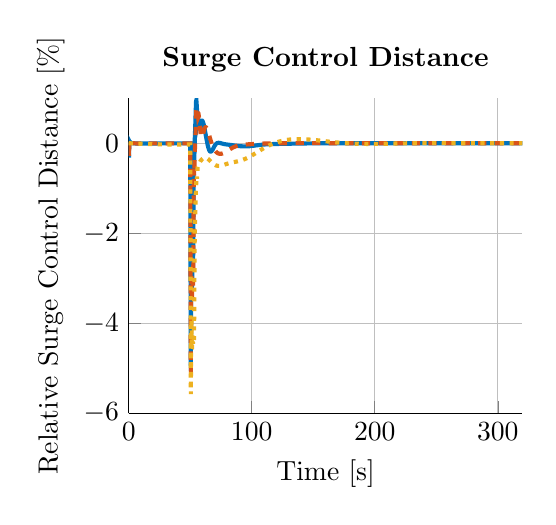
\begin{tikzpicture}

\begin{axis}[%
width=5cm,
height=4cm,
at={(0\linewidth,0\linewidth)},
scale only axis,
xmin=0,
xmax=320,
xlabel={Time [s]},
xmajorgrids,
ymin=-6,
ymax=1,
ylabel={Relative Surge Control Distance [\%]},
ymajorgrids,
axis background/.style={fill=white},
title style={font=\bfseries},
title={Surge Control Distance},
axis x line*=bottom,
axis y line*=left
]
\addplot [color=mycolor1,solid,line width=1.5pt,forget plot]
  table[row sep=crcr]{%
0	-0.0970099999999992\\
0.25	-0.31776\\
0.5	0.0485000000000007\\
% 0.75	0.0541400000000003\\
% 1	-0.00875999999999877\\
1.25	0.00740000000000052\\
1.5	0.01755\\
1.75	0.00960000000000072\\
2	0.00655000000000072\\
2.25	0.00689000000000028\\
2.5	0.00555000000000128\\
2.75	0.00388000000000055\\
3	0.0028100000000002\\
3.25	0.00186000000000064\\
3.5	0.000899999999999679\\
3.75	6.00000000012813e-05\\
4	-0.000669999999999504\\
4.25	-0.00131999999999977\\
4.5	-0.00190999999999875\\
4.75	-0.00244\\
5	-0.00292999999999921\\
5.25	-0.00337000000000032\\
5.5	-0.00376999999999938\\
5.75	-0.00411999999999857\\
6	-0.00441999999999965\\
6.25	-0.00467999999999869\\
6.5	-0.00488\\
6.75	-0.00503999999999927\\
7	-0.00514999999999866\\
7.25	-0.0052399999999988\\
7.5	-0.00530000000000008\\
7.75	-0.00534999999999997\\
8	-0.00539000000000023\\
8.25	-0.00541999999999909\\
8.5	-0.00544999999999973\\
8.75	-0.00545999999999935\\
9	-0.00546999999999898\\
9.25	-0.00545999999999935\\
9.5	-0.00544000000000011\\
9.75	-0.00539000000000023\\
10	-0.00532999999999895\\
10.25	-0.00526999999999944\\
10.5	-0.00520000000000032\\
10.75	-0.00512999999999941\\
11	-0.00506999999999991\\
11.25	-0.00500999999999863\\
11.5	-0.00497000000000014\\
11.75	-0.00492999999999988\\
12	-0.00488999999999962\\
12.25	-0.00484999999999935\\
12.5	-0.00479999999999947\\
12.75	-0.00474999999999959\\
13	-0.00469000000000008\\
13.25	-0.00461999999999918\\
13.5	-0.00455000000000005\\
13.75	-0.00448999999999877\\
14	-0.00443999999999889\\
14.25	-0.00439999999999863\\
14.5	-0.00436999999999976\\
14.75	-0.00433999999999912\\
15	-0.00431999999999988\\
15.25	-0.00429999999999886\\
15.5	-0.00427999999999962\\
15.75	-0.00424999999999898\\
16	-0.00420999999999871\\
16.25	-0.00417000000000023\\
16.5	-0.00412999999999997\\
16.75	-0.0040899999999997\\
17	-0.00404999999999944\\
17.25	-0.0040300000000002\\
17.5	-0.00400999999999918\\
17.75	-0.00399999999999956\\
18	-0.00398999999999994\\
18.25	-0.00398999999999994\\
18.5	-0.00398000000000032\\
18.75	-0.0039599999999993\\
19	-0.00394000000000005\\
19.25	-0.00390999999999941\\
19.5	-0.00387999999999877\\
19.75	-0.00384999999999991\\
20	-0.00381999999999927\\
20.25	-0.00380000000000003\\
20.5	-0.00378999999999863\\
20.75	-0.00377999999999901\\
21	-0.00377999999999901\\
21.25	-0.00377999999999901\\
21.5	-0.00376999999999938\\
21.75	-0.00375999999999976\\
22	-0.00373999999999874\\
22.25	-0.00370999999999988\\
22.5	-0.00367999999999924\\
22.75	-0.0036499999999986\\
23	-0.00362999999999936\\
23.25	-0.00361000000000011\\
23.5	-0.00358999999999909\\
23.75	-0.00358999999999909\\
24	-0.00357999999999947\\
24.25	-0.00357999999999947\\
24.5	-0.00356999999999985\\
24.75	-0.00356000000000023\\
25	-0.00353999999999921\\
25.25	-0.00351999999999997\\
25.5	-0.00348999999999933\\
25.75	-0.00345999999999869\\
26	-0.00342999999999982\\
26.25	-0.0034099999999988\\
26.5	-0.00339999999999918\\
26.75	-0.00338999999999956\\
27	-0.00338999999999956\\
27.25	-0.00337999999999994\\
27.5	-0.00337999999999994\\
27.75	-0.00337000000000032\\
28	-0.0033499999999993\\
28.25	-0.00333000000000006\\
28.5	-0.00329999999999941\\
28.75	-0.00326999999999877\\
29	-0.00324999999999953\\
29.25	-0.00323000000000029\\
29.5	-0.00320999999999927\\
29.75	-0.00320999999999927\\
30	-0.00319999999999965\\
30.25	-0.00320999999999927\\
30.5	-0.00319999999999965\\
30.75	-0.00319999999999965\\
31	-0.00317999999999863\\
31.25	-0.00316999999999901\\
31.5	-0.00314000000000014\\
31.75	-0.0031099999999995\\
32	-0.00309000000000026\\
32.25	-0.00306999999999924\\
32.5	-0.00305999999999962\\
32.75	-0.00305999999999962\\
33	-0.00305999999999962\\
33.25	-0.00305999999999962\\
33.5	-0.00306999999999924\\
33.75	-0.00305999999999962\\
34	-0.00305999999999962\\
34.25	-0.0030399999999986\\
34.5	-0.00301999999999936\\
34.75	-0.00300000000000011\\
35	-0.00296999999999947\\
35.25	-0.00295999999999985\\
35.5	-0.00295000000000023\\
35.75	-0.00295000000000023\\
36	-0.00295999999999985\\
36.25	-0.00295999999999985\\
36.5	-0.00296999999999947\\
36.75	-0.00296999999999947\\
37	-0.00296999999999947\\
37.25	-0.00295999999999985\\
37.5	-0.00293999999999883\\
37.75	-0.00291999999999959\\
38	-0.00289999999999857\\
38.25	-0.00288999999999895\\
38.5	-0.00287999999999933\\
38.75	-0.00287999999999933\\
39	-0.00288999999999895\\
39.25	-0.00290999999999997\\
39.5	-0.00291999999999959\\
39.75	-0.00292999999999921\\
40	-0.00291999999999959\\
40.25	-0.00290999999999997\\
40.5	-0.00289999999999857\\
40.75	-0.00287999999999933\\
41	-0.00286000000000008\\
41.25	-0.00284999999999869\\
41.5	-0.00284999999999869\\
41.75	-0.00284999999999869\\
42	-0.00286999999999971\\
42.25	-0.00287999999999933\\
42.5	-0.00289999999999857\\
42.75	-0.00290999999999997\\
43	-0.00290999999999997\\
43.25	-0.00289999999999857\\
43.5	-0.00288999999999895\\
43.75	-0.00286999999999971\\
44	-0.00284999999999869\\
44.25	-0.00283999999999907\\
44.5	-0.00283999999999907\\
44.75	-0.00284999999999869\\
45	-0.00286000000000008\\
45.25	-0.00288999999999895\\
45.5	-0.00290999999999997\\
45.75	-0.00291999999999959\\
46	-0.00291999999999959\\
46.25	-0.00290999999999997\\
46.5	-0.00289999999999857\\
46.75	-0.00287999999999933\\
47	-0.00286000000000008\\
47.25	-0.00284999999999869\\
47.5	-0.00284999999999869\\
47.75	-0.00286000000000008\\
48	-0.00287999999999933\\
48.25	-0.00290999999999997\\
48.5	-0.00292999999999921\\
48.75	-0.00293999999999883\\
49	-0.00295000000000023\\
49.25	-0.00293999999999883\\
49.5	-0.00291999999999959\\
49.75	-0.00289999999999857\\
50	-0.00287999999999933\\
50.25	-2.77916\\
50.5	-5.05865\\
50.75	-3.23165\\
51	-2.68995\\
51.25	-3.30532\\
51.5	-3.10962\\
51.75	-2.76589\\
52	-2.79788\\
52.25	-2.84727\\
52.5	-2.23862\\
52.75	-0.72666\\
53	-0.289249999999999\\
53.25	-0.39575\\
53.5	-0.128729999999999\\
53.75	0.138570000000001\\
54	0.309560000000001\\
54.25	0.51932\\
54.5	0.75141\\
54.75	0.92952\\
55	0.958270000000001\\
55.25	0.85941\\
55.5	0.747640000000001\\
55.75	0.572740000000001\\
56	0.471160000000001\\
56.25	0.511200000000001\\
56.5	0.53909\\
56.75	0.50972\\
57	0.481300000000001\\
57.25	0.467120000000001\\
57.5	0.45491\\
57.75	0.434140000000001\\
58	0.41464\\
58.25	0.41826\\
58.5	0.440330000000001\\
58.75	0.462670000000001\\
59	0.479850000000001\\
59.25	0.49292\\
59.5	0.500150000000001\\
59.75	0.499920000000001\\
60	0.49268\\
60.25	0.47955\\
60.5	0.461220000000001\\
60.75	0.438130000000001\\
61	0.410960000000001\\
61.25	0.380560000000001\\
61.5	0.347670000000001\\
61.75	0.31287\\
62	0.276670000000001\\
62.25	0.23958\\
62.5	0.20199\\
62.75	0.16431\\
63	0.126890000000001\\
63.25	0.090110000000001\\
63.5	0.054310000000001\\
63.75	0.0198499999999999\\
64	-0.012929999999999\\
64.25	-0.0437199999999986\\
64.5	-0.0721999999999987\\
64.75	-0.0980600000000003\\
65	-0.120999999999999\\
65.25	-0.14073\\
65.5	-0.15696\\
65.75	-0.169449999999999\\
66	-0.178139999999999\\
66.25	-0.183199999999999\\
66.5	-0.185099999999999\\
66.75	-0.184419999999999\\
67	-0.181539999999999\\
67.25	-0.176609999999999\\
67.5	-0.16968\\
67.75	-0.160889999999999\\
68	-0.15049\\
68.25	-0.138809999999999\\
68.5	-0.126189999999999\\
68.75	-0.113019999999999\\
69	-0.0996299999999994\\
69.25	-0.0863599999999991\\
69.5	-0.0734699999999986\\
69.75	-0.0612099999999991\\
70	-0.0497399999999999\\
70.25	-0.0392099999999989\\
70.5	-0.0297000000000001\\
70.75	-0.0212699999999995\\
71	-0.0139199999999988\\
71.25	-0.00765999999999956\\
71.5	-0.00244999999999962\\
71.75	0.00176000000000087\\
72	0.00505000000000067\\
72.25	0.00747000000000142\\
72.5	0.00912000000000113\\
72.75	0.0100700000000007\\
73	0.0104199999999999\\
73.25	0.0102400000000014\\
73.5	0.00961999999999996\\
73.75	0.00863999999999976\\
74	0.00735000000000063\\
74.25	0.00584000000000096\\
74.5	0.00415000000000099\\
74.75	0.00234000000000023\\
75	0.000460000000000349\\
75.25	-0.00146999999999942\\
75.5	-0.00339999999999918\\
75.75	-0.00531999999999933\\
76	-0.00718999999999959\\
76.25	-0.00899999999999856\\
76.5	-0.0107499999999998\\
76.75	-0.0124199999999988\\
77	-0.014009999999999\\
77.25	-0.015509999999999\\
77.5	-0.01694\\
77.75	-0.018279999999999\\
78	-0.0195499999999988\\
78.25	-0.0207499999999996\\
78.5	-0.0218799999999995\\
78.75	-0.0229599999999994\\
79	-0.0239899999999995\\
79.25	-0.0249699999999997\\
79.5	-0.0259099999999997\\
79.75	-0.0268299999999986\\
80	-0.0277199999999986\\
80.25	-0.0285999999999991\\
80.5	-0.0294600000000003\\
80.75	-0.0303100000000001\\
81	-0.0311599999999999\\
81.25	-0.0320099999999996\\
81.5	-0.0328699999999991\\
81.75	-0.0337300000000003\\
82	-0.0345899999999997\\
82.25	-0.0354700000000001\\
82.5	-0.0363600000000002\\
82.75	-0.0372599999999998\\
83	-0.0381599999999995\\
83.25	-0.0390800000000002\\
83.5	-0.0400099999999988\\
83.75	-0.0409499999999987\\
84	-0.0419\\
84.25	-0.0428599999999992\\
84.5	-0.0438200000000002\\
84.75	-0.044789999999999\\
85	-0.0457599999999996\\
85.25	-0.0467300000000002\\
85.5	-0.047699999999999\\
85.75	-0.0486799999999992\\
86	-0.0496400000000001\\
86.25	-0.0506099999999989\\
86.5	-0.0515600000000003\\
86.75	-0.0525099999999998\\
87	-0.0534400000000002\\
87.25	-0.0543699999999987\\
87.5	-0.0552799999999998\\
87.75	-0.0561699999999998\\
88	-0.0570500000000003\\
88.25	-0.0579099999999997\\
88.5	-0.0587499999999999\\
88.75	-0.059569999999999\\
89	-0.0603599999999993\\
89.25	-0.0611299999999986\\
89.5	-0.061869999999999\\
89.75	-0.0625799999999987\\
90	-0.0632599999999996\\
90.25	-0.0639199999999995\\
90.5	-0.0645399999999992\\
90.75	-0.0651299999999999\\
91	-0.06569\\
91.25	-0.0662099999999999\\
91.5	-0.0666899999999995\\
91.75	-0.0671400000000002\\
92	-0.0675499999999989\\
92.25	-0.0679199999999991\\
92.5	-0.068249999999999\\
92.75	-0.0685399999999987\\
93	-0.0687899999999999\\
93.25	-0.0690099999999987\\
93.5	-0.0691799999999994\\
93.75	-0.0693000000000001\\
94	-0.0693900000000003\\
94.25	-0.0694299999999988\\
94.5	-0.0694400000000002\\
94.75	-0.0693999999999999\\
95	-0.0693199999999994\\
95.25	-0.0691999999999986\\
95.5	-0.0690299999999997\\
95.75	-0.0688300000000002\\
96	-0.0685899999999986\\
96.25	-0.0682999999999989\\
96.5	-0.0679799999999986\\
96.75	-0.0676199999999998\\
97	-0.0672199999999989\\
97.25	-0.0667899999999992\\
97.5	-0.0663199999999993\\
97.75	-0.0658199999999987\\
98	-0.0652799999999996\\
98.25	-0.0647199999999994\\
98.5	-0.0641199999999991\\
98.75	-0.0634899999999998\\
99	-0.0628399999999996\\
99.25	-0.0621599999999987\\
99.5	-0.0614499999999989\\
99.75	-0.0607199999999999\\
100	-0.0599699999999999\\
100.25	-0.0591999999999988\\
100.5	-0.0584100000000003\\
100.75	-0.057599999999999\\
101	-0.0567799999999998\\
101.25	-0.0559399999999997\\
101.5	-0.0550899999999999\\
101.75	-0.0542299999999987\\
102	-0.0533599999999996\\
102.25	-0.0524799999999992\\
102.5	-0.0515999999999988\\
102.75	-0.0507099999999987\\
103	-0.0498199999999986\\
103.25	-0.048919999999999\\
103.5	-0.0480299999999989\\
103.75	-0.0471299999999992\\
104	-0.0462399999999992\\
104.25	-0.0453499999999991\\
104.5	-0.0444699999999987\\
104.75	-0.04359\\
105	-0.0427199999999992\\
105.25	-0.0418599999999998\\
105.5	-0.04101\\
105.75	-0.0401600000000002\\
106	-0.0393299999999996\\
106.25	-0.0385099999999987\\
106.5	-0.0376999999999992\\
106.75	-0.0369099999999989\\
107	-0.03613\\
107.25	-0.0353599999999989\\
107.5	-0.0346099999999989\\
107.75	-0.0338799999999999\\
108	-0.0331599999999987\\
108.25	-0.032449999999999\\
108.5	-0.0317699999999999\\
108.75	-0.0310999999999986\\
109	-0.0304500000000001\\
109.25	-0.0298199999999991\\
109.5	-0.0291999999999994\\
109.75	-0.0285999999999991\\
110	-0.0280199999999997\\
110.25	-0.0274599999999996\\
110.5	-0.0269099999999991\\
110.75	-0.0263899999999992\\
111	-0.025879999999999\\
111.25	-0.0253800000000002\\
111.5	-0.0249100000000002\\
111.75	-0.0244499999999999\\
112	-0.0239999999999991\\
112.25	-0.0235699999999994\\
112.5	-0.023159999999999\\
112.75	-0.0227599999999999\\
113	-0.0223800000000001\\
113.25	-0.0220099999999999\\
113.5	-0.0216599999999989\\
113.75	-0.0213199999999993\\
114	-0.0209899999999994\\
114.25	-0.0206799999999987\\
114.5	-0.0203699999999998\\
114.75	-0.0200800000000001\\
115	-0.0198\\
115.25	-0.0195399999999992\\
115.5	-0.0192800000000002\\
115.75	-0.019029999999999\\
116	-0.0187899999999992\\
116.25	-0.018559999999999\\
116.5	-0.0183400000000002\\
116.75	-0.0181199999999997\\
117	-0.0179200000000002\\
117.25	-0.0177199999999988\\
117.5	-0.0175199999999993\\
117.75	-0.017339999999999\\
118	-0.0171599999999987\\
118.25	-0.0169800000000002\\
118.5	-0.0168099999999995\\
118.75	-0.0166399999999989\\
119	-0.0164799999999996\\
119.25	-0.0163199999999986\\
119.5	-0.0161699999999989\\
119.75	-0.0160199999999993\\
120	-0.0158699999999996\\
120.25	-0.01572\\
120.5	-0.0155799999999999\\
120.75	-0.0154399999999999\\
121	-0.0152999999999999\\
121.25	-0.0151599999999998\\
121.5	-0.0150199999999998\\
121.75	-0.0148799999999998\\
122	-0.0147499999999994\\
122.25	-0.0146099999999993\\
122.5	-0.0144799999999989\\
122.75	-0.0143500000000003\\
123	-0.0142100000000003\\
123.25	-0.0140799999999999\\
123.5	-0.0139499999999995\\
123.75	-0.0138199999999991\\
124	-0.013679999999999\\
124.25	-0.0135499999999986\\
124.5	-0.01342\\
124.75	-0.01328\\
125	-0.0131499999999996\\
125.25	-0.0130099999999995\\
125.5	-0.0128799999999991\\
125.75	-0.0127399999999991\\
126	-0.0126099999999987\\
126.25	-0.0124699999999986\\
126.5	-0.0123299999999986\\
126.75	-0.0122\\
127	-0.01206\\
127.25	-0.0119199999999999\\
127.5	-0.0117799999999999\\
127.75	-0.0116399999999999\\
128	-0.0114999999999998\\
128.25	-0.0113599999999998\\
128.5	-0.0112199999999998\\
128.75	-0.0110799999999998\\
129	-0.0109399999999997\\
129.25	-0.0107900000000001\\
129.5	-0.01065\\
129.75	-0.01051\\
130	-0.01037\\
130.25	-0.01023\\
130.5	-0.0100800000000003\\
130.75	-0.00994000000000028\\
131	-0.00980000000000025\\
131.25	-0.00966000000000022\\
131.5	-0.00952000000000019\\
131.75	-0.00938000000000017\\
132	-0.00922999999999874\\
132.25	-0.00908999999999871\\
132.5	-0.00894999999999868\\
132.75	-0.00882000000000005\\
133	-0.00868000000000002\\
133.25	-0.00853999999999999\\
133.5	-0.00839999999999996\\
133.75	-0.00825999999999993\\
134	-0.00812999999999953\\
134.25	-0.0079899999999995\\
134.5	-0.00785999999999909\\
134.75	-0.00772999999999868\\
135	-0.00758999999999865\\
135.25	-0.00746000000000002\\
135.5	-0.00732999999999961\\
135.75	-0.00719999999999921\\
136	-0.0070800000000002\\
136.25	-0.00694999999999979\\
136.5	-0.00681999999999938\\
136.75	-0.0066999999999986\\
137	-0.00657999999999959\\
137.25	-0.0064599999999988\\
137.5	-0.00633999999999979\\
137.75	-0.006219999999999\\
138	-0.00609999999999999\\
138.25	-0.00597999999999921\\
138.5	-0.00586999999999982\\
138.75	-0.00574999999999903\\
139	-0.00563999999999965\\
139.25	-0.00553000000000026\\
139.5	-0.00541999999999909\\
139.75	-0.0053099999999997\\
140	-0.00520999999999994\\
140.25	-0.00509999999999877\\
140.5	-0.00499999999999901\\
140.75	-0.00489999999999924\\
141	-0.00479999999999947\\
141.25	-0.0046999999999997\\
141.5	-0.00459999999999994\\
141.75	-0.00450000000000017\\
142	-0.00441000000000003\\
142.25	-0.00431000000000026\\
142.5	-0.00422000000000011\\
142.75	-0.00412999999999997\\
143	-0.00403999999999982\\
143.25	-0.00394999999999968\\
143.5	-0.00386999999999915\\
143.75	-0.00377999999999901\\
144	-0.00370000000000026\\
144.25	-0.00361999999999973\\
144.5	-0.00353999999999921\\
144.75	-0.00345999999999869\\
145	-0.00337999999999994\\
145.25	-0.00329999999999941\\
145.5	-0.00321999999999889\\
145.75	-0.00314999999999976\\
146	-0.00306999999999924\\
146.25	-0.00300000000000011\\
146.5	-0.00292999999999921\\
146.75	-0.00286000000000008\\
147	-0.00278999999999918\\
147.25	-0.00272000000000006\\
147.5	-0.00264999999999915\\
147.75	-0.00258999999999965\\
148	-0.00251999999999875\\
148.25	-0.00245999999999924\\
148.5	-0.00239999999999974\\
148.75	-0.00232999999999883\\
149	-0.00226999999999933\\
149.25	-0.00220999999999982\\
149.5	-0.00215000000000032\\
149.75	-0.00209999999999866\\
150	-0.00203999999999915\\
150.25	-0.00197999999999965\\
150.5	-0.00192999999999977\\
150.75	-0.00187000000000026\\
151	-0.0018199999999986\\
151.25	-0.0017599999999991\\
151.5	-0.00170999999999921\\
151.75	-0.00165999999999933\\
152	-0.00160999999999945\\
152.25	-0.00155999999999956\\
152.5	-0.00150999999999968\\
152.75	-0.00145999999999979\\
153	-0.00140999999999991\\
153.25	-0.00136000000000003\\
153.5	-0.00131999999999977\\
153.75	-0.00126999999999988\\
154	-0.00122\\
154.25	-0.00117999999999974\\
154.5	-0.00112999999999985\\
154.75	-0.00108999999999959\\
155	-0.00104999999999933\\
155.25	-0.00100999999999907\\
155.5	-0.000959999999999184\\
155.75	-0.000919999999998922\\
156	-0.00087999999999866\\
156.25	-0.000840000000000174\\
156.5	-0.000799999999999912\\
156.75	-0.00075999999999965\\
157	-0.000719999999999388\\
157.25	-0.000679999999999126\\
157.5	-0.000650000000000261\\
157.75	-0.000609999999999999\\
158	-0.000569999999999737\\
158.25	-0.000539999999999097\\
158.5	-0.000499999999998835\\
158.75	-0.00046999999999997\\
159	-0.000429999999999708\\
159.25	-0.000399999999999068\\
159.5	-0.000359999999998806\\
159.75	-0.000329999999999941\\
160	-0.000299999999999301\\
160.25	-0.000259999999999039\\
160.5	-0.000230000000000175\\
160.75	-0.000199999999999534\\
161	-0.000169999999998893\\
161.25	-0.000140000000000029\\
161.5	-0.000109999999999388\\
161.75	-7.99999999987477e-05\\
162	-4.99999999998835e-05\\
162.25	-1.99999999992428e-05\\
162.5	1.00000000013978e-05\\
162.75	4.0000000000262e-05\\
163	7.00000000009027e-05\\
163.25	9.00000000001455e-05\\
163.5	0.000120000000000786\\
163.75	0.000150000000001427\\
164	0.00017000000000067\\
164.25	0.00020000000000131\\
164.5	0.000230000000000175\\
164.75	0.000250000000001194\\
165	0.000280000000000058\\
165.25	0.000300000000001077\\
165.5	0.00032000000000032\\
165.75	0.000350000000000961\\
166	0.000370000000000203\\
166.25	0.000390000000001223\\
166.5	0.000420000000000087\\
166.75	0.000440000000001106\\
167	0.000460000000000349\\
167.25	0.000480000000001368\\
167.5	0.000500000000000611\\
167.75	0.000519999999999854\\
168	0.000540000000000873\\
168.25	0.000560000000000116\\
168.5	0.000580000000001135\\
168.75	0.000600000000000378\\
169	0.000620000000001397\\
169.25	0.00064000000000064\\
169.5	0.000659999999999883\\
169.75	0.000670000000001281\\
170	0.000690000000000524\\
170.25	0.000709999999999766\\
170.5	0.000730000000000786\\
170.75	0.000740000000000407\\
171	0.000760000000001426\\
171.25	0.000770000000001048\\
171.5	0.00079000000000029\\
171.75	0.00081000000000131\\
172	0.000820000000000931\\
172.25	0.000830000000000553\\
172.5	0.000849999999999795\\
172.75	0.000860000000001193\\
173	0.000880000000000436\\
173.25	0.000890000000000057\\
173.5	0.000899999999999679\\
173.75	0.000920000000000698\\
174	0.000930000000000319\\
174.25	0.000939999999999941\\
174.5	0.000950000000001339\\
174.75	0.00096000000000096\\
175	0.000970000000000582\\
175.25	0.000989999999999824\\
175.5	0.00100000000000122\\
175.75	0.00101000000000084\\
176	0.00102000000000046\\
176.25	0.00103000000000009\\
176.5	0.00103999999999971\\
176.75	0.00105000000000111\\
177	0.00105000000000111\\
177.25	0.00106000000000073\\
177.5	0.00107000000000035\\
177.75	0.00107999999999997\\
178	0.00109000000000137\\
178.25	0.00110000000000099\\
178.5	0.00110000000000099\\
178.75	0.00111000000000061\\
179	0.00112000000000023\\
179.25	0.00112000000000023\\
179.5	0.00112999999999985\\
179.75	0.00114000000000125\\
180	0.00114000000000125\\
180.25	0.00115000000000087\\
180.5	0.00116000000000049\\
180.75	0.00116000000000049\\
181	0.00117000000000012\\
181.25	0.00117000000000012\\
181.5	0.00117999999999974\\
181.75	0.00117999999999974\\
182	0.00119000000000113\\
182.25	0.00119000000000113\\
182.5	0.00119000000000113\\
182.75	0.00120000000000076\\
183	0.00120000000000076\\
183.25	0.00120000000000076\\
183.5	0.00121000000000038\\
183.75	0.00121000000000038\\
184	0.00121000000000038\\
184.25	0.00122\\
184.5	0.00122\\
184.75	0.00122\\
185	0.00122\\
185.25	0.0012300000000014\\
185.5	0.0012300000000014\\
185.75	0.0012300000000014\\
186	0.0012300000000014\\
186.25	0.0012300000000014\\
186.5	0.0012300000000014\\
186.75	0.00124000000000102\\
187	0.00124000000000102\\
187.25	0.00124000000000102\\
187.5	0.00124000000000102\\
187.75	0.00124000000000102\\
188	0.00124000000000102\\
188.25	0.00124000000000102\\
188.5	0.00124000000000102\\
188.75	0.00124000000000102\\
189	0.00124000000000102\\
189.25	0.00124000000000102\\
189.5	0.00124000000000102\\
189.75	0.00124000000000102\\
190	0.00124000000000102\\
190.25	0.00124000000000102\\
190.5	0.00124000000000102\\
190.75	0.0012300000000014\\
191	0.0012300000000014\\
191.25	0.0012300000000014\\
191.5	0.0012300000000014\\
191.75	0.0012300000000014\\
192	0.0012300000000014\\
192.25	0.0012300000000014\\
192.5	0.00122\\
192.75	0.00122\\
193	0.00122\\
193.25	0.00122\\
193.5	0.00122\\
193.75	0.00121000000000038\\
194	0.00121000000000038\\
194.25	0.00121000000000038\\
194.5	0.00121000000000038\\
194.75	0.00120000000000076\\
195	0.00120000000000076\\
195.25	0.00120000000000076\\
195.5	0.00119000000000113\\
195.75	0.00119000000000113\\
196	0.00119000000000113\\
196.25	0.00117999999999974\\
196.5	0.00117999999999974\\
196.75	0.00117999999999974\\
197	0.00117000000000012\\
197.25	0.00117000000000012\\
197.5	0.00117000000000012\\
197.75	0.00116000000000049\\
198	0.00116000000000049\\
198.25	0.00116000000000049\\
198.5	0.00115000000000087\\
198.75	0.00115000000000087\\
199	0.00114000000000125\\
199.25	0.00114000000000125\\
199.5	0.00114000000000125\\
199.75	0.00112999999999985\\
200	0.00112999999999985\\
200.25	0.00112000000000023\\
200.5	0.00112000000000023\\
200.75	0.00111000000000061\\
201	0.00111000000000061\\
201.25	0.00111000000000061\\
201.5	0.00110000000000099\\
201.75	0.00110000000000099\\
202	0.00109000000000137\\
202.25	0.00109000000000137\\
202.5	0.00107999999999997\\
202.75	0.00107999999999997\\
203	0.00107000000000035\\
203.25	0.00107000000000035\\
203.5	0.00106000000000073\\
203.75	0.00106000000000073\\
204	0.00105000000000111\\
204.25	0.00105000000000111\\
204.5	0.00103999999999971\\
204.75	0.00103999999999971\\
205	0.00103000000000009\\
205.25	0.00103000000000009\\
205.5	0.00102000000000046\\
205.75	0.00102000000000046\\
206	0.00101000000000084\\
206.25	0.00101000000000084\\
206.5	0.00100000000000122\\
206.75	0.00100000000000122\\
207	0.000989999999999824\\
207.25	0.000980000000000203\\
207.5	0.000980000000000203\\
207.75	0.000970000000000582\\
208	0.000970000000000582\\
208.25	0.00096000000000096\\
208.5	0.00096000000000096\\
208.75	0.000950000000001339\\
209	0.000950000000001339\\
209.25	0.000939999999999941\\
209.5	0.000930000000000319\\
209.75	0.000930000000000319\\
210	0.000920000000000698\\
210.25	0.000920000000000698\\
210.5	0.000910000000001077\\
210.75	0.000910000000001077\\
211	0.000899999999999679\\
211.25	0.000890000000000057\\
211.5	0.000890000000000057\\
211.75	0.000880000000000436\\
212	0.000880000000000436\\
212.25	0.000870000000000815\\
212.5	0.000870000000000815\\
212.75	0.000860000000001193\\
213	0.000849999999999795\\
213.25	0.000849999999999795\\
213.5	0.000840000000000174\\
213.75	0.000840000000000174\\
214	0.000830000000000553\\
214.25	0.000830000000000553\\
214.5	0.000820000000000931\\
214.75	0.00081000000000131\\
215	0.00081000000000131\\
215.25	0.000799999999999912\\
215.5	0.000799999999999912\\
215.75	0.00079000000000029\\
216	0.000780000000000669\\
216.25	0.000780000000000669\\
216.5	0.000770000000001048\\
216.75	0.000770000000001048\\
217	0.000760000000001426\\
217.25	0.000760000000001426\\
217.5	0.000750000000000028\\
217.75	0.000740000000000407\\
218	0.000740000000000407\\
218.25	0.000730000000000786\\
218.5	0.000730000000000786\\
218.75	0.000720000000001164\\
219	0.000720000000001164\\
219.25	0.000709999999999766\\
219.5	0.000700000000000145\\
219.75	0.000700000000000145\\
220	0.000690000000000524\\
220.25	0.000690000000000524\\
220.5	0.000680000000000902\\
220.75	0.000680000000000902\\
221	0.000670000000001281\\
221.25	0.000659999999999883\\
221.5	0.000659999999999883\\
221.75	0.000650000000000261\\
222	0.000650000000000261\\
222.25	0.00064000000000064\\
222.5	0.00064000000000064\\
222.75	0.000630000000001019\\
223	0.000630000000001019\\
223.25	0.000620000000001397\\
223.5	0.000620000000001397\\
223.75	0.000609999999999999\\
224	0.000600000000000378\\
224.25	0.000600000000000378\\
224.5	0.000590000000000757\\
224.75	0.000590000000000757\\
225	0.000580000000001135\\
225.25	0.000580000000001135\\
225.5	0.000569999999999737\\
225.75	0.000569999999999737\\
226	0.000560000000000116\\
226.25	0.000560000000000116\\
226.5	0.000550000000000495\\
226.75	0.000550000000000495\\
227	0.000540000000000873\\
227.25	0.000540000000000873\\
227.5	0.000530000000001252\\
227.75	0.000530000000001252\\
228	0.000519999999999854\\
228.25	0.000510000000000232\\
228.5	0.000510000000000232\\
228.75	0.000500000000000611\\
229	0.000500000000000611\\
229.25	0.00049000000000099\\
229.5	0.00049000000000099\\
229.75	0.000480000000001368\\
230	0.000480000000001368\\
230.25	0.000480000000001368\\
230.5	0.00046999999999997\\
230.75	0.00046999999999997\\
231	0.000460000000000349\\
231.25	0.000460000000000349\\
231.5	0.000450000000000728\\
231.75	0.000450000000000728\\
232	0.000440000000001106\\
232.25	0.000440000000001106\\
232.5	0.000429999999999708\\
232.75	0.000429999999999708\\
233	0.000420000000000087\\
233.25	0.000420000000000087\\
233.5	0.000410000000000466\\
233.75	0.000410000000000466\\
234	0.000400000000000844\\
234.25	0.000400000000000844\\
234.5	0.000400000000000844\\
234.75	0.000390000000001223\\
235	0.000390000000001223\\
235.25	0.000379999999999825\\
235.5	0.000379999999999825\\
235.75	0.000370000000000203\\
236	0.000370000000000203\\
236.25	0.000370000000000203\\
236.5	0.000360000000000582\\
236.75	0.000360000000000582\\
237	0.000350000000000961\\
237.25	0.000350000000000961\\
237.5	0.000340000000001339\\
237.75	0.000340000000001339\\
238	0.000340000000001339\\
238.25	0.000329999999999941\\
238.5	0.000329999999999941\\
238.75	0.00032000000000032\\
239	0.00032000000000032\\
239.25	0.00032000000000032\\
239.5	0.000310000000000699\\
239.75	0.000310000000000699\\
240	0.000300000000001077\\
240.25	0.000300000000001077\\
240.5	0.000300000000001077\\
240.75	0.000289999999999679\\
241	0.000289999999999679\\
241.25	0.000289999999999679\\
241.5	0.000280000000000058\\
241.75	0.000280000000000058\\
242	0.000270000000000437\\
242.25	0.000270000000000437\\
242.5	0.000270000000000437\\
242.75	0.000260000000000815\\
243	0.000260000000000815\\
243.25	0.000260000000000815\\
243.5	0.000250000000001194\\
243.75	0.000250000000001194\\
244	0.000250000000001194\\
244.25	0.000239999999999796\\
244.5	0.000239999999999796\\
244.75	0.000239999999999796\\
245	0.000230000000000175\\
245.25	0.000230000000000175\\
245.5	0.000230000000000175\\
245.75	0.000220000000000553\\
246	0.000220000000000553\\
246.25	0.000220000000000553\\
246.5	0.000210000000000932\\
246.75	0.000210000000000932\\
247	0.000210000000000932\\
247.25	0.00020000000000131\\
247.5	0.00020000000000131\\
247.75	0.00020000000000131\\
248	0.00020000000000131\\
248.25	0.000189999999999912\\
248.5	0.000189999999999912\\
248.75	0.000189999999999912\\
249	0.000180000000000291\\
249.25	0.000180000000000291\\
249.5	0.000180000000000291\\
249.75	0.000180000000000291\\
250	0.00017000000000067\\
250.25	0.00017000000000067\\
250.5	0.00017000000000067\\
250.75	0.000160000000001048\\
251	0.000160000000001048\\
251.25	0.000160000000001048\\
251.5	0.000160000000001048\\
251.75	0.000150000000001427\\
252	0.000150000000001427\\
252.25	0.000150000000001427\\
252.5	0.000150000000001427\\
252.75	0.000140000000000029\\
253	0.000140000000000029\\
253.25	0.000140000000000029\\
253.5	0.000140000000000029\\
253.75	0.000130000000000408\\
254	0.000130000000000408\\
254.25	0.000130000000000408\\
254.5	0.000130000000000408\\
254.75	0.000120000000000786\\
255	0.000120000000000786\\
255.25	0.000120000000000786\\
255.5	0.000120000000000786\\
255.75	0.000120000000000786\\
256	0.000110000000001165\\
256.25	0.000110000000001165\\
256.5	0.000110000000001165\\
256.75	0.000110000000001165\\
257	9.99999999997669e-05\\
257.25	9.99999999997669e-05\\
257.5	9.99999999997669e-05\\
257.75	9.99999999997669e-05\\
258	9.99999999997669e-05\\
258.25	9.00000000001455e-05\\
258.5	9.00000000001455e-05\\
258.75	9.00000000001455e-05\\
259	9.00000000001455e-05\\
259.25	9.00000000001455e-05\\
259.5	8.00000000005241e-05\\
259.75	8.00000000005241e-05\\
260	8.00000000005241e-05\\
260.25	8.00000000005241e-05\\
260.5	8.00000000005241e-05\\
260.75	8.00000000005241e-05\\
261	7.00000000009027e-05\\
261.25	7.00000000009027e-05\\
261.5	7.00000000009027e-05\\
261.75	7.00000000009027e-05\\
262	7.00000000009027e-05\\
262.25	7.00000000009027e-05\\
262.5	6.00000000012813e-05\\
262.75	6.00000000012813e-05\\
263	6.00000000012813e-05\\
263.25	6.00000000012813e-05\\
263.5	6.00000000012813e-05\\
263.75	6.00000000012813e-05\\
264	4.99999999998835e-05\\
264.25	4.99999999998835e-05\\
264.5	4.99999999998835e-05\\
264.75	4.99999999998835e-05\\
265	4.99999999998835e-05\\
265.25	4.99999999998835e-05\\
265.5	4.99999999998835e-05\\
265.75	4.0000000000262e-05\\
266	4.0000000000262e-05\\
266.25	4.0000000000262e-05\\
266.5	4.0000000000262e-05\\
266.75	4.0000000000262e-05\\
267	4.0000000000262e-05\\
267.25	4.0000000000262e-05\\
267.5	3.00000000006406e-05\\
267.75	3.00000000006406e-05\\
268	3.00000000006406e-05\\
268.25	3.00000000006406e-05\\
268.5	3.00000000006406e-05\\
268.75	3.00000000006406e-05\\
269	3.00000000006406e-05\\
269.25	3.00000000006406e-05\\
269.5	2.00000000010192e-05\\
269.75	2.00000000010192e-05\\
270	2.00000000010192e-05\\
270.25	2.00000000010192e-05\\
270.5	2.00000000010192e-05\\
270.75	2.00000000010192e-05\\
271	2.00000000010192e-05\\
271.25	2.00000000010192e-05\\
271.5	2.00000000010192e-05\\
271.75	2.00000000010192e-05\\
272	1.00000000013978e-05\\
272.25	1.00000000013978e-05\\
272.5	1.00000000013978e-05\\
272.75	1.00000000013978e-05\\
273	1.00000000013978e-05\\
273.25	1.00000000013978e-05\\
273.5	1.00000000013978e-05\\
273.75	1.00000000013978e-05\\
274	1.00000000013978e-05\\
274.25	1.00000000013978e-05\\
274.5	0\\
274.75	0\\
275	0\\
275.25	0\\
275.5	0\\
275.75	0\\
276	0\\
276.25	0\\
276.5	0\\
276.75	0\\
277	0\\
277.25	0\\
277.5	0\\
277.75	0\\
278	-9.99999999962142e-06\\
278.25	-9.99999999962142e-06\\
278.5	-9.99999999962142e-06\\
278.75	-9.99999999962142e-06\\
279	-9.99999999962142e-06\\
279.25	-9.99999999962142e-06\\
279.5	-9.99999999962142e-06\\
279.75	-9.99999999962142e-06\\
280	-9.99999999962142e-06\\
280.25	-9.99999999962142e-06\\
280.5	-9.99999999962142e-06\\
280.75	-9.99999999962142e-06\\
281	-9.99999999962142e-06\\
281.25	-9.99999999962142e-06\\
281.5	-9.99999999962142e-06\\
281.75	-9.99999999962142e-06\\
282	-9.99999999962142e-06\\
282.25	-1.99999999992428e-05\\
282.5	-1.99999999992428e-05\\
282.75	-1.99999999992428e-05\\
283	-1.99999999992428e-05\\
283.25	-1.99999999992428e-05\\
283.5	-1.99999999992428e-05\\
283.75	-1.99999999992428e-05\\
284	-1.99999999992428e-05\\
284.25	-1.99999999992428e-05\\
284.5	-1.99999999992428e-05\\
284.75	-1.99999999992428e-05\\
285	-1.99999999992428e-05\\
285.25	-1.99999999992428e-05\\
285.5	-1.99999999992428e-05\\
285.75	-1.99999999992428e-05\\
286	-1.99999999992428e-05\\
286.25	-1.99999999992428e-05\\
286.5	-1.99999999992428e-05\\
286.75	-1.99999999992428e-05\\
287	-1.99999999992428e-05\\
287.25	-1.99999999992428e-05\\
287.5	-1.99999999992428e-05\\
287.75	-1.99999999992428e-05\\
288	-1.99999999992428e-05\\
288.25	-1.99999999992428e-05\\
288.5	-1.99999999992428e-05\\
288.75	-2.99999999988643e-05\\
289	-2.99999999988643e-05\\
289.25	-2.99999999988643e-05\\
289.5	-2.99999999988643e-05\\
289.75	-2.99999999988643e-05\\
290	-2.99999999988643e-05\\
290.25	-2.99999999988643e-05\\
290.5	-2.99999999988643e-05\\
290.75	-2.99999999988643e-05\\
291	-2.99999999988643e-05\\
291.25	-2.99999999988643e-05\\
291.5	-2.99999999988643e-05\\
291.75	-2.99999999988643e-05\\
292	-2.99999999988643e-05\\
292.25	-2.99999999988643e-05\\
292.5	-2.99999999988643e-05\\
292.75	-2.99999999988643e-05\\
293	-2.99999999988643e-05\\
293.25	-2.99999999988643e-05\\
293.5	-2.99999999988643e-05\\
293.75	-2.99999999988643e-05\\
294	-2.99999999988643e-05\\
294.25	-2.99999999988643e-05\\
294.5	-2.99999999988643e-05\\
294.75	-2.99999999988643e-05\\
295	-2.99999999988643e-05\\
295.25	-2.99999999988643e-05\\
295.5	-2.99999999988643e-05\\
295.75	-2.99999999988643e-05\\
296	-2.99999999988643e-05\\
296.25	-2.99999999988643e-05\\
296.5	-2.99999999988643e-05\\
296.75	-2.99999999988643e-05\\
297	-2.99999999988643e-05\\
297.25	-2.99999999988643e-05\\
297.5	-2.99999999988643e-05\\
297.75	-2.99999999988643e-05\\
298	-2.99999999988643e-05\\
298.25	-2.99999999988643e-05\\
298.5	-2.99999999988643e-05\\
298.75	-2.99999999988643e-05\\
299	-2.99999999988643e-05\\
299.25	-2.99999999988643e-05\\
299.5	-2.99999999988643e-05\\
299.75	-2.99999999988643e-05\\
300	-2.99999999988643e-05\\
300.25	-2.99999999988643e-05\\
300.5	-2.99999999988643e-05\\
300.75	-2.99999999988643e-05\\
301	-2.99999999988643e-05\\
301.25	-2.99999999988643e-05\\
301.5	-2.99999999988643e-05\\
301.75	-2.99999999988643e-05\\
302	-2.99999999988643e-05\\
302.25	-2.99999999988643e-05\\
302.5	-2.99999999988643e-05\\
302.75	-2.99999999988643e-05\\
303	-2.99999999988643e-05\\
303.25	-2.99999999988643e-05\\
303.5	-2.99999999988643e-05\\
303.75	-2.99999999988643e-05\\
304	-2.99999999988643e-05\\
304.25	-2.99999999988643e-05\\
304.5	-2.99999999988643e-05\\
304.75	-2.99999999988643e-05\\
305	-2.99999999988643e-05\\
305.25	-2.99999999988643e-05\\
305.5	-2.99999999988643e-05\\
305.75	-2.99999999988643e-05\\
306	-2.99999999988643e-05\\
306.25	-2.99999999988643e-05\\
306.5	-2.99999999988643e-05\\
306.75	-2.99999999988643e-05\\
307	-2.99999999988643e-05\\
307.25	-2.99999999988643e-05\\
307.5	-2.99999999988643e-05\\
307.75	-2.99999999988643e-05\\
308	-2.99999999988643e-05\\
308.25	-2.99999999988643e-05\\
308.5	-2.99999999988643e-05\\
308.75	-2.99999999988643e-05\\
309	-2.99999999988643e-05\\
309.25	-2.99999999988643e-05\\
309.5	-2.99999999988643e-05\\
309.75	-2.99999999988643e-05\\
310	-2.99999999988643e-05\\
310.25	-2.99999999988643e-05\\
310.5	-2.99999999988643e-05\\
310.75	-2.99999999988643e-05\\
311	-2.99999999988643e-05\\
311.25	-2.99999999988643e-05\\
311.5	-2.99999999988643e-05\\
311.75	-2.99999999988643e-05\\
312	-2.99999999988643e-05\\
312.25	-2.99999999988643e-05\\
312.5	-2.99999999988643e-05\\
312.75	-2.99999999988643e-05\\
313	-2.99999999988643e-05\\
313.25	-2.99999999988643e-05\\
313.5	-2.99999999988643e-05\\
313.75	-2.99999999988643e-05\\
314	-2.99999999988643e-05\\
314.25	-2.99999999988643e-05\\
314.5	-2.99999999988643e-05\\
314.75	-2.99999999988643e-05\\
315	-2.99999999988643e-05\\
315.25	-2.99999999988643e-05\\
315.5	-2.99999999988643e-05\\
315.75	-2.99999999988643e-05\\
316	-2.99999999988643e-05\\
316.25	-2.99999999988643e-05\\
316.5	-2.99999999988643e-05\\
316.75	-2.99999999988643e-05\\
317	-2.99999999988643e-05\\
317.25	-2.99999999988643e-05\\
317.5	-2.99999999988643e-05\\
317.75	-2.99999999988643e-05\\
318	-2.99999999988643e-05\\
318.25	-2.99999999988643e-05\\
318.5	-1.99999999992428e-05\\
318.75	-1.99999999992428e-05\\
319	-1.99999999992428e-05\\
319.25	-1.99999999992428e-05\\
319.5	-1.99999999992428e-05\\
319.75	-1.99999999992428e-05\\
320	-1.99999999992428e-05\\
320.25	-1.99999999992428e-05\\
320.5	-1.99999999992428e-05\\
320.75	-1.99999999992428e-05\\
321	-1.99999999992428e-05\\
321.25	-1.99999999992428e-05\\
321.5	-1.99999999992428e-05\\
321.75	-1.99999999992428e-05\\
322	-1.99999999992428e-05\\
322.25	-1.99999999992428e-05\\
322.5	-1.99999999992428e-05\\
322.75	-1.99999999992428e-05\\
323	-1.99999999992428e-05\\
323.25	-1.99999999992428e-05\\
323.5	-1.99999999992428e-05\\
323.75	-1.99999999992428e-05\\
324	-1.99999999992428e-05\\
324.25	-1.99999999992428e-05\\
324.5	-1.99999999992428e-05\\
324.75	-1.99999999992428e-05\\
325	-1.99999999992428e-05\\
325.25	-1.99999999992428e-05\\
325.5	-1.99999999992428e-05\\
325.75	-1.99999999992428e-05\\
326	-1.99999999992428e-05\\
326.25	-1.99999999992428e-05\\
326.5	-1.99999999992428e-05\\
326.75	-1.99999999992428e-05\\
327	-1.99999999992428e-05\\
327.25	-1.99999999992428e-05\\
327.5	-1.99999999992428e-05\\
327.75	-1.99999999992428e-05\\
328	-1.99999999992428e-05\\
328.25	-1.99999999992428e-05\\
328.5	-1.99999999992428e-05\\
328.75	-1.99999999992428e-05\\
329	-1.99999999992428e-05\\
329.25	-1.99999999992428e-05\\
329.5	-1.99999999992428e-05\\
329.75	-1.99999999992428e-05\\
330	-1.99999999992428e-05\\
330.25	-1.99999999992428e-05\\
330.5	-1.99999999992428e-05\\
330.75	-1.99999999992428e-05\\
331	-1.99999999992428e-05\\
331.25	-1.99999999992428e-05\\
331.5	-1.99999999992428e-05\\
331.75	-1.99999999992428e-05\\
332	-1.99999999992428e-05\\
332.25	-1.99999999992428e-05\\
332.5	-1.99999999992428e-05\\
332.75	-1.99999999992428e-05\\
333	-1.99999999992428e-05\\
333.25	-1.99999999992428e-05\\
333.5	-1.99999999992428e-05\\
333.75	-1.99999999992428e-05\\
334	-1.99999999992428e-05\\
334.25	-1.99999999992428e-05\\
334.5	-1.99999999992428e-05\\
334.75	-1.99999999992428e-05\\
335	-1.99999999992428e-05\\
335.25	-1.99999999992428e-05\\
335.5	-1.99999999992428e-05\\
335.75	-1.99999999992428e-05\\
336	-9.99999999962142e-06\\
336.25	-9.99999999962142e-06\\
336.5	-9.99999999962142e-06\\
336.75	-9.99999999962142e-06\\
337	-9.99999999962142e-06\\
337.25	-9.99999999962142e-06\\
337.5	-9.99999999962142e-06\\
337.75	-9.99999999962142e-06\\
338	-9.99999999962142e-06\\
338.25	-9.99999999962142e-06\\
338.5	-9.99999999962142e-06\\
338.75	-9.99999999962142e-06\\
339	-9.99999999962142e-06\\
339.25	-9.99999999962142e-06\\
339.5	-9.99999999962142e-06\\
339.75	-9.99999999962142e-06\\
340	-9.99999999962142e-06\\
340.25	-9.99999999962142e-06\\
340.5	-9.99999999962142e-06\\
340.75	-9.99999999962142e-06\\
341	-9.99999999962142e-06\\
341.25	-9.99999999962142e-06\\
341.5	-9.99999999962142e-06\\
341.75	-9.99999999962142e-06\\
342	-9.99999999962142e-06\\
342.25	-9.99999999962142e-06\\
342.5	-9.99999999962142e-06\\
342.75	-9.99999999962142e-06\\
343	-9.99999999962142e-06\\
343.25	-9.99999999962142e-06\\
343.5	-9.99999999962142e-06\\
343.75	-9.99999999962142e-06\\
344	-9.99999999962142e-06\\
344.25	-9.99999999962142e-06\\
344.5	-9.99999999962142e-06\\
344.75	-9.99999999962142e-06\\
345	-9.99999999962142e-06\\
345.25	-9.99999999962142e-06\\
345.5	-9.99999999962142e-06\\
345.75	-9.99999999962142e-06\\
346	-9.99999999962142e-06\\
346.25	-9.99999999962142e-06\\
346.5	-9.99999999962142e-06\\
346.75	-9.99999999962142e-06\\
347	-9.99999999962142e-06\\
347.25	-9.99999999962142e-06\\
347.5	-9.99999999962142e-06\\
347.75	-9.99999999962142e-06\\
348	-9.99999999962142e-06\\
348.25	-9.99999999962142e-06\\
348.5	-9.99999999962142e-06\\
348.75	-9.99999999962142e-06\\
349	-9.99999999962142e-06\\
349.25	-9.99999999962142e-06\\
349.5	-9.99999999962142e-06\\
349.75	-9.99999999962142e-06\\
350	-9.99999999962142e-06\\
350.25	-9.99999999962142e-06\\
350.5	-9.99999999962142e-06\\
350.75	-9.99999999962142e-06\\
351	-9.99999999962142e-06\\
351.25	-9.99999999962142e-06\\
351.5	-9.99999999962142e-06\\
351.75	-9.99999999962142e-06\\
352	-9.99999999962142e-06\\
352.25	-9.99999999962142e-06\\
352.5	-9.99999999962142e-06\\
352.75	-9.99999999962142e-06\\
353	-9.99999999962142e-06\\
353.25	-9.99999999962142e-06\\
353.5	-9.99999999962142e-06\\
353.75	-9.99999999962142e-06\\
354	-9.99999999962142e-06\\
354.25	-9.99999999962142e-06\\
354.5	-9.99999999962142e-06\\
354.75	-9.99999999962142e-06\\
355	-9.99999999962142e-06\\
355.25	-9.99999999962142e-06\\
355.5	-9.99999999962142e-06\\
355.75	-9.99999999962142e-06\\
356	-9.99999999962142e-06\\
356.25	-9.99999999962142e-06\\
356.5	-9.99999999962142e-06\\
356.75	-9.99999999962142e-06\\
357	-9.99999999962142e-06\\
357.25	-9.99999999962142e-06\\
357.5	-9.99999999962142e-06\\
357.75	-9.99999999962142e-06\\
358	-9.99999999962142e-06\\
358.25	-9.99999999962142e-06\\
358.5	-9.99999999962142e-06\\
358.75	-9.99999999962142e-06\\
359	-9.99999999962142e-06\\
359.25	-9.99999999962142e-06\\
359.5	0\\
359.75	0\\
360	0\\
360.25	0\\
360.5	0\\
360.75	0\\
361	0\\
361.25	0\\
361.5	0\\
361.75	0\\
362	0\\
362.25	0\\
362.5	0\\
362.75	0\\
363	0\\
363.25	0\\
363.5	0\\
363.75	0\\
364	0\\
364.25	0\\
364.5	0\\
364.75	0\\
365	0\\
365.25	0\\
365.5	0\\
365.75	0\\
366	0\\
366.25	0\\
366.5	0\\
366.75	0\\
367	0\\
367.25	0\\
367.5	0\\
367.75	0\\
368	0\\
368.25	0\\
368.5	0\\
368.75	0\\
369	0\\
369.25	0\\
369.5	0\\
369.75	0\\
370	0\\
370.25	0\\
370.5	0\\
370.75	0\\
371	0\\
371.25	0\\
371.5	0\\
371.75	0\\
372	0\\
372.25	0\\
372.5	0\\
372.75	0\\
373	0\\
373.25	0\\
373.5	0\\
373.75	0\\
374	0\\
374.25	0\\
374.5	0\\
374.75	0\\
375	0\\
375.25	0\\
375.5	0\\
375.75	0\\
376	0\\
376.25	0\\
376.5	0\\
376.75	0\\
377	0\\
377.25	0\\
377.5	0\\
377.75	0\\
378	0\\
378.25	0\\
378.5	0\\
378.75	0\\
379	0\\
379.25	0\\
379.5	0\\
379.75	0\\
380	0\\
380.25	0\\
380.5	0\\
380.75	0\\
381	0\\
381.25	0\\
381.5	0\\
381.75	0\\
382	0\\
382.25	0\\
382.5	0\\
382.75	0\\
383	0\\
383.25	0\\
383.5	0\\
383.75	0\\
384	0\\
384.25	0\\
384.5	0\\
384.75	0\\
385	0\\
385.25	0\\
385.5	0\\
385.75	0\\
386	0\\
386.25	0\\
386.5	0\\
386.75	0\\
387	0\\
387.25	0\\
387.5	0\\
387.75	0\\
388	0\\
388.25	0\\
388.5	0\\
388.75	0\\
389	0\\
389.25	0\\
389.5	0\\
389.75	0\\
390	0\\
390.25	0\\
390.5	0\\
390.75	0\\
391	0\\
391.25	0\\
391.5	0\\
391.75	0\\
392	0\\
392.25	0\\
392.5	0\\
392.75	0\\
393	0\\
393.25	0\\
393.5	0\\
393.75	0\\
394	0\\
394.25	0\\
394.5	0\\
394.75	0\\
395	0\\
395.25	0\\
395.5	0\\
395.75	0\\
396	0\\
396.25	0\\
396.5	0\\
396.75	0\\
397	0\\
397.25	0\\
397.5	0\\
397.75	0\\
398	0\\
398.25	0\\
398.5	0\\
398.75	0\\
399	0\\
399.25	0\\
399.5	0\\
399.75	0\\
400	0\\
400.25	0\\
400.5	0\\
400.75	0\\
401	0\\
401.25	0\\
401.5	0\\
401.75	0\\
402	0\\
402.25	0\\
402.5	0\\
402.75	0\\
403	0\\
403.25	0\\
403.5	0\\
403.75	0\\
404	0\\
404.25	0\\
404.5	0\\
404.75	0\\
405	0\\
405.25	0\\
405.5	0\\
405.75	0\\
406	0\\
406.25	0\\
406.5	0\\
406.75	0\\
407	0\\
407.25	0\\
407.5	0\\
407.75	0\\
408	0\\
408.25	0\\
408.5	0\\
408.75	0\\
409	0\\
409.25	0\\
409.5	0\\
409.75	0\\
410	0\\
410.25	0\\
410.5	0\\
410.75	0\\
411	0\\
411.25	0\\
411.5	0\\
411.75	0\\
412	0\\
412.25	0\\
412.5	0\\
412.75	0\\
413	0\\
413.25	0\\
413.5	0\\
413.75	0\\
414	0\\
414.25	0\\
414.5	0\\
414.75	0\\
415	0\\
415.25	0\\
415.5	0\\
415.75	0\\
416	0\\
416.25	0\\
416.5	0\\
416.75	0\\
417	0\\
417.25	0\\
417.5	0\\
417.75	0\\
418	0\\
418.25	0\\
418.5	0\\
418.75	0\\
419	0\\
419.25	0\\
419.5	0\\
419.75	0\\
420	0\\
420.25	0\\
420.5	0\\
420.75	0\\
421	0\\
421.25	0\\
421.5	0\\
421.75	0\\
422	0\\
422.25	0\\
422.5	0\\
422.75	0\\
423	0\\
423.25	0\\
423.5	0\\
423.75	0\\
424	0\\
424.25	0\\
424.5	0\\
424.75	0\\
425	0\\
425.25	0\\
425.5	0\\
425.75	0\\
426	0\\
426.25	0\\
426.5	0\\
426.75	0\\
427	0\\
427.25	0\\
427.5	0\\
427.75	0\\
428	0\\
428.25	0\\
428.5	0\\
428.75	0\\
429	0\\
429.25	0\\
429.5	0\\
429.75	0\\
430	0\\
430.25	0\\
430.5	0\\
430.75	0\\
431	0\\
431.25	0\\
431.5	0\\
431.75	0\\
432	0\\
432.25	0\\
432.5	0\\
432.75	0\\
433	0\\
433.25	0\\
433.5	0\\
433.75	0\\
434	0\\
434.25	0\\
434.5	0\\
434.75	0\\
435	0\\
435.25	0\\
435.5	0\\
435.75	0\\
436	0\\
436.25	0\\
436.5	0\\
436.75	0\\
437	0\\
437.25	0\\
437.5	0\\
437.75	0\\
438	0\\
438.25	0\\
438.5	0\\
438.75	0\\
439	0\\
439.25	0\\
439.5	0\\
439.75	0\\
440	0\\
440.25	0\\
440.5	0\\
440.75	0\\
441	0\\
441.25	0\\
441.5	0\\
441.75	0\\
442	0\\
442.25	0\\
442.5	0\\
442.75	0\\
443	0\\
443.25	0\\
443.5	0\\
443.75	0\\
444	0\\
444.25	0\\
444.5	0\\
444.75	0\\
445	0\\
445.25	0\\
445.5	0\\
445.75	0\\
446	0\\
446.25	0\\
446.5	0\\
446.75	0\\
447	0\\
447.25	0\\
447.5	0\\
447.75	0\\
448	0\\
448.25	0\\
448.5	0\\
448.75	0\\
449	0\\
449.25	0\\
449.5	0\\
449.75	0\\
450	0\\
450.25	0\\
450.5	0\\
450.75	0\\
451	0\\
451.25	0\\
451.5	0\\
451.75	0\\
452	0\\
452.25	0\\
452.5	0\\
452.75	0\\
453	0\\
453.25	0\\
453.5	0\\
453.75	0\\
454	0\\
454.25	0\\
454.5	0\\
454.75	0\\
455	0\\
455.25	0\\
455.5	0\\
455.75	0\\
456	0\\
456.25	0\\
456.5	0\\
456.75	0\\
457	0\\
457.25	0\\
457.5	0\\
457.75	0\\
458	0\\
458.25	0\\
458.5	0\\
458.75	0\\
459	0\\
459.25	0\\
459.5	0\\
459.75	0\\
460	0\\
460.25	0\\
460.5	0\\
460.75	0\\
461	0\\
461.25	0\\
461.5	0\\
461.75	0\\
462	0\\
462.25	0\\
462.5	0\\
462.75	0\\
463	0\\
463.25	0\\
463.5	0\\
463.75	0\\
464	0\\
464.25	0\\
464.5	0\\
464.75	0\\
465	0\\
465.25	0\\
465.5	0\\
465.75	0\\
466	0\\
466.25	0\\
466.5	0\\
466.75	0\\
467	0\\
467.25	0\\
467.5	0\\
467.75	0\\
468	0\\
468.25	0\\
468.5	0\\
468.75	0\\
469	0\\
469.25	0\\
469.5	0\\
469.75	0\\
470	0\\
470.25	0\\
470.5	0\\
470.75	0\\
471	0\\
471.25	0\\
471.5	0\\
471.75	0\\
472	0\\
472.25	0\\
472.5	0\\
472.75	0\\
473	0\\
473.25	0\\
473.5	0\\
473.75	0\\
474	0\\
474.25	0\\
474.5	0\\
474.75	0\\
475	0\\
475.25	0\\
475.5	0\\
475.75	0\\
476	0\\
476.25	0\\
476.5	0\\
476.75	0\\
477	0\\
477.25	0\\
477.5	0\\
477.75	0\\
478	0\\
478.25	0\\
478.5	0\\
478.75	0\\
479	0\\
479.25	0\\
479.5	0\\
479.75	0\\
480	0\\
480.25	0\\
480.5	0\\
480.75	0\\
481	0\\
481.25	0\\
481.5	0\\
481.75	0\\
482	0\\
482.25	0\\
482.5	0\\
482.75	0\\
483	0\\
483.25	0\\
483.5	0\\
483.75	0\\
484	0\\
484.25	0\\
484.5	0\\
484.75	0\\
485	0\\
485.25	0\\
485.5	0\\
485.75	0\\
486	0\\
486.25	0\\
486.5	0\\
486.75	0\\
487	0\\
487.25	0\\
487.5	0\\
487.75	0\\
488	0\\
488.25	0\\
488.5	0\\
488.75	0\\
489	0\\
489.25	0\\
489.5	0\\
489.75	0\\
490	0\\
490.25	0\\
490.5	0\\
490.75	0\\
491	0\\
491.25	0\\
491.5	0\\
491.75	0\\
492	0\\
492.25	0\\
492.5	0\\
492.75	0\\
493	0\\
493.25	0\\
493.5	0\\
493.75	0\\
494	0\\
494.25	0\\
494.5	0\\
494.75	0\\
495	0\\
495.25	0\\
495.5	0\\
495.75	0\\
496	0\\
496.25	0\\
496.5	0\\
496.75	0\\
497	0\\
497.25	0\\
497.5	0\\
497.75	0\\
498	0\\
498.25	0\\
498.5	0\\
498.75	0\\
499	0\\
499.25	0\\
499.5	0\\
499.75	0\\
};
\addplot [color=mycolor2,dashed,line width=1.5pt,forget plot]
  table[row sep=crcr]{%
0	-0.0970099999999992\\
0.25	-0.319129999999999\\
0.5	0.0460900000000013\\
0.75	0.05321\\
1	-0.0088999999999988\\
1.25	0.00727000000000011\\
1.5	0.0177800000000001\\
1.75	0.0102700000000002\\
2	0.00746000000000002\\
2.25	0.00801000000000052\\
2.5	0.00688000000000066\\
2.75	0.00536000000000136\\
3	0.00438000000000116\\
3.25	0.0034900000000011\\
3.5	0.00253999999999976\\
3.75	0.00168000000000035\\
4	0.000910000000001077\\
4.25	0.00020000000000131\\
4.5	-0.000449999999998951\\
4.75	-0.00103999999999971\\
5	-0.0015799999999988\\
5.25	-0.00206000000000017\\
5.5	-0.00248999999999988\\
5.75	-0.00287999999999933\\
6	-0.00323000000000029\\
6.25	-0.00354999999999883\\
6.5	-0.00382999999999889\\
6.75	-0.00406999999999869\\
7	-0.00427999999999962\\
7.25	-0.00446999999999953\\
7.5	-0.00461999999999918\\
7.75	-0.00473999999999997\\
8	-0.00483999999999973\\
8.25	-0.00492000000000026\\
8.5	-0.00497999999999976\\
8.75	-0.00502000000000002\\
9	-0.00503999999999927\\
9.25	-0.00506000000000029\\
9.5	-0.00506000000000029\\
9.75	-0.00504999999999889\\
10	-0.00503999999999927\\
10.25	-0.00500999999999863\\
10.5	-0.00497999999999976\\
10.75	-0.00494999999999912\\
11	-0.00490999999999886\\
11.25	-0.00485999999999898\\
11.5	-0.00480999999999909\\
11.75	-0.00474999999999959\\
12	-0.00469000000000008\\
12.25	-0.0046400000000002\\
12.5	-0.00457999999999892\\
12.75	-0.00451999999999941\\
13	-0.00445999999999991\\
13.25	-0.00439999999999863\\
13.5	-0.00434999999999874\\
13.75	-0.00428999999999924\\
14	-0.00423999999999936\\
14.25	-0.00417999999999985\\
14.5	-0.00412999999999997\\
14.75	-0.00408000000000008\\
15	-0.0040300000000002\\
15.25	-0.00398000000000032\\
15.5	-0.00392999999999866\\
15.75	-0.00387999999999877\\
16	-0.00384000000000029\\
16.25	-0.00380000000000003\\
16.5	-0.00375999999999976\\
16.75	-0.0037199999999995\\
17	-0.00367999999999924\\
17.25	-0.00363999999999898\\
17.5	-0.00361000000000011\\
17.75	-0.00357999999999947\\
18	-0.00353999999999921\\
18.25	-0.00350999999999857\\
18.5	-0.00347999999999971\\
18.75	-0.00345999999999869\\
19	-0.00342999999999982\\
19.25	-0.00339999999999918\\
19.5	-0.00337999999999994\\
19.75	-0.00335999999999892\\
20	-0.00333999999999968\\
20.25	-0.00330999999999904\\
20.5	-0.00328999999999979\\
20.75	-0.00328000000000017\\
21	-0.00325999999999915\\
21.25	-0.00323999999999991\\
21.5	-0.00321999999999889\\
21.75	-0.00320999999999927\\
22	-0.00319000000000003\\
22.25	-0.00317999999999863\\
22.5	-0.00316999999999901\\
22.75	-0.00314999999999976\\
23	-0.00314000000000014\\
23.25	-0.00312999999999874\\
23.5	-0.00311999999999912\\
23.75	-0.0031099999999995\\
24	-0.00309999999999988\\
24.25	-0.00309999999999988\\
24.5	-0.00309000000000026\\
24.75	-0.00307999999999886\\
25	-0.00307999999999886\\
25.25	-0.00306999999999924\\
25.5	-0.00306999999999924\\
25.75	-0.00305999999999962\\
26	-0.00305999999999962\\
26.25	-0.00305\\
26.5	-0.00305\\
26.75	-0.00305\\
27	-0.00305\\
27.25	-0.00305\\
27.5	-0.00305\\
27.75	-0.00305\\
28	-0.00305\\
28.25	-0.00305\\
28.5	-0.00305\\
28.75	-0.00305\\
29	-0.00305999999999962\\
29.25	-0.00305999999999962\\
29.5	-0.00305999999999962\\
29.75	-0.00305999999999962\\
30	-0.00306999999999924\\
30.25	-0.00306999999999924\\
30.5	-0.00307999999999886\\
30.75	-0.00307999999999886\\
31	-0.00309000000000026\\
31.25	-0.00309000000000026\\
31.5	-0.00309999999999988\\
31.75	-0.00309999999999988\\
32	-0.0031099999999995\\
32.25	-0.00311999999999912\\
32.5	-0.00311999999999912\\
32.75	-0.00312999999999874\\
33	-0.00312999999999874\\
33.25	-0.00314000000000014\\
33.5	-0.00314999999999976\\
33.75	-0.00314999999999976\\
34	-0.00315999999999939\\
34.25	-0.00316999999999901\\
34.5	-0.00316999999999901\\
34.75	-0.00317999999999863\\
35	-0.00319000000000003\\
35.25	-0.00319000000000003\\
35.5	-0.00319999999999965\\
35.75	-0.00319999999999965\\
36	-0.00320999999999927\\
36.25	-0.00321999999999889\\
36.5	-0.00321999999999889\\
36.75	-0.00323000000000029\\
37	-0.00323000000000029\\
37.25	-0.00323999999999991\\
37.5	-0.00323999999999991\\
37.75	-0.00324999999999953\\
38	-0.00324999999999953\\
38.25	-0.00325999999999915\\
38.5	-0.00325999999999915\\
38.75	-0.00326999999999877\\
39	-0.00326999999999877\\
39.25	-0.00326999999999877\\
39.5	-0.00328000000000017\\
39.75	-0.00328000000000017\\
40	-0.00328000000000017\\
40.25	-0.00328000000000017\\
40.5	-0.00328999999999979\\
40.75	-0.00328999999999979\\
41	-0.00328999999999979\\
41.25	-0.00328999999999979\\
41.5	-0.00328999999999979\\
41.75	-0.00329999999999941\\
42	-0.00329999999999941\\
42.25	-0.00329999999999941\\
42.5	-0.00329999999999941\\
42.75	-0.00329999999999941\\
43	-0.00329999999999941\\
43.25	-0.00329999999999941\\
43.5	-0.00329999999999941\\
43.75	-0.00329999999999941\\
44	-0.00329999999999941\\
44.25	-0.00329999999999941\\
44.5	-0.00329999999999941\\
44.75	-0.00329999999999941\\
45	-0.00328999999999979\\
45.25	-0.00328999999999979\\
45.5	-0.00328999999999979\\
45.75	-0.00328999999999979\\
46	-0.00328999999999979\\
46.25	-0.00328999999999979\\
46.5	-0.00328000000000017\\
46.75	-0.00328000000000017\\
47	-0.00328000000000017\\
47.25	-0.00328000000000017\\
47.5	-0.00328000000000017\\
47.75	-0.00326999999999877\\
48	-0.00326999999999877\\
48.25	-0.00326999999999877\\
48.5	-0.00326999999999877\\
48.75	-0.00325999999999915\\
49	-0.00325999999999915\\
49.25	-0.00325999999999915\\
49.5	-0.00325999999999915\\
49.75	-0.00325999999999915\\
50	-0.00324999999999953\\
50.25	-2.78574\\
50.5	-5.08938\\
50.75	-3.36652\\
51	-2.95481\\
51.25	-3.56188\\
51.5	-3.37647\\
51.75	-3.07036\\
52	-3.12297\\
52.25	-3.12183\\
52.5	-2.81816\\
52.75	-1.34351\\
53	-0.569399999999999\\
53.25	-0.72974\\
53.5	-0.501639999999999\\
53.75	-0.175129999999999\\
54	-0.00672999999999924\\
54.25	0.124470000000001\\
54.5	0.37031\\
54.75	0.62124\\
55	0.767150000000001\\
55.25	0.8071\\
55.5	0.803840000000001\\
55.75	0.79331\\
56	0.76746\\
56.25	0.657780000000001\\
56.5	0.57873\\
56.75	0.59585\\
57	0.601840000000001\\
57.25	0.555910000000001\\
57.5	0.49188\\
57.75	0.427710000000001\\
58	0.354560000000001\\
58.25	0.27036\\
58.5	0.193800000000001\\
58.75	0.14659\\
59	0.127550000000001\\
59.25	0.123380000000001\\
59.5	0.128080000000001\\
59.75	0.141440000000001\\
60	0.16165\\
60.25	0.185640000000001\\
60.5	0.21176\\
60.75	0.23925\\
61	0.266760000000001\\
61.25	0.29236\\
61.5	0.314530000000001\\
61.75	0.332360000000001\\
62	0.34539\\
62.25	0.353440000000001\\
62.5	0.35661\\
62.75	0.355210000000001\\
63	0.34967\\
63.25	0.340440000000001\\
63.5	0.32799\\
63.75	0.312810000000001\\
64	0.29538\\
64.25	0.27613\\
64.5	0.255470000000001\\
64.75	0.23376\\
65	0.211310000000001\\
65.25	0.188420000000001\\
65.5	0.16531\\
65.75	0.14222\\
66	0.11931\\
66.25	0.0967400000000005\\
66.5	0.0746599999999997\\
66.75	0.0531500000000005\\
67	0.0323100000000007\\
67.25	0.0122100000000014\\
67.5	-0.00709999999999944\\
67.75	-0.0255799999999997\\
68	-0.0432199999999998\\
68.25	-0.0599799999999995\\
68.5	-0.0758700000000001\\
68.75	-0.0908800000000003\\
69	-0.105029999999999\\
69.25	-0.118309999999999\\
69.5	-0.130739999999999\\
69.75	-0.142339999999999\\
70	-0.153129999999999\\
70.25	-0.16313\\
70.5	-0.17235\\
70.75	-0.180829999999999\\
71	-0.18859\\
71.25	-0.195639999999999\\
71.5	-0.202019999999999\\
71.75	-0.20775\\
72	-0.21285\\
72.25	-0.21735\\
72.5	-0.221259999999999\\
72.75	-0.22462\\
73	-0.227449999999999\\
73.25	-0.22976\\
73.5	-0.23159\\
73.75	-0.23295\\
74	-0.23387\\
74.25	-0.23436\\
74.5	-0.234459999999999\\
74.75	-0.23417\\
75	-0.23352\\
75.25	-0.232539999999999\\
75.5	-0.231229999999999\\
75.75	-0.22962\\
76	-0.22772\\
76.25	-0.22556\\
76.5	-0.22315\\
76.75	-0.220509999999999\\
77	-0.217649999999999\\
77.25	-0.214589999999999\\
77.5	-0.211349999999999\\
77.75	-0.207949999999999\\
78	-0.204389999999999\\
78.25	-0.20069\\
78.5	-0.19687\\
78.75	-0.192939999999999\\
79	-0.188909999999999\\
79.25	-0.184799999999999\\
79.5	-0.180619999999999\\
79.75	-0.17639\\
80	-0.172099999999999\\
80.25	-0.167789999999999\\
80.5	-0.163449999999999\\
80.75	-0.159089999999999\\
81	-0.154739999999999\\
81.25	-0.15039\\
81.5	-0.146059999999999\\
81.75	-0.14176\\
82	-0.13749\\
82.25	-0.13327\\
82.5	-0.129099999999999\\
82.75	-0.124979999999999\\
83	-0.12093\\
83.25	-0.116949999999999\\
83.5	-0.11304\\
83.75	-0.109219999999999\\
84	-0.10548\\
84.25	-0.10183\\
84.5	-0.0982699999999994\\
84.75	-0.094809999999999\\
85	-0.0914399999999986\\
85.25	-0.0881799999999995\\
85.5	-0.0850200000000001\\
85.75	-0.0819599999999987\\
86	-0.0790100000000002\\
86.25	-0.0761599999999998\\
86.5	-0.0734099999999991\\
86.75	-0.0707699999999996\\
87	-0.0682299999999998\\
87.25	-0.0657999999999994\\
87.5	-0.0634599999999992\\
87.75	-0.0612199999999987\\
88	-0.0590799999999998\\
88.25	-0.0570399999999989\\
88.5	-0.0550899999999999\\
88.75	-0.0532299999999992\\
89	-0.0514499999999991\\
89.25	-0.0497599999999991\\
89.5	-0.0481599999999993\\
89.75	-0.0466299999999986\\
90	-0.0451800000000002\\
90.25	-0.0437999999999992\\
90.5	-0.042489999999999\\
90.75	-0.0412499999999998\\
91	-0.0400700000000001\\
91.25	-0.0389499999999998\\
91.5	-0.0378899999999991\\
91.75	-0.0368899999999996\\
92	-0.0359299999999987\\
92.25	-0.0350199999999994\\
92.5	-0.03416\\
92.75	-0.033339999999999\\
93	-0.0325600000000001\\
93.25	-0.0318199999999997\\
93.5	-0.03111\\
93.75	-0.0304299999999991\\
94	-0.0297799999999988\\
94.25	-0.0291599999999992\\
94.5	-0.0285700000000002\\
94.75	-0.0279999999999987\\
95	-0.02745\\
95.25	-0.0269099999999991\\
95.5	-0.0263999999999989\\
95.75	-0.0259\\
96	-0.0254199999999987\\
96.25	-0.0249499999999987\\
96.5	-0.0244999999999997\\
96.75	-0.024049999999999\\
97	-0.0236099999999997\\
97.25	-0.02318\\
97.5	-0.0227599999999999\\
97.75	-0.0223499999999994\\
98	-0.021939999999999\\
98.25	-0.0215399999999999\\
98.5	-0.0211499999999987\\
98.75	-0.0207599999999992\\
99	-0.0203699999999998\\
99.25	-0.01999\\
99.5	-0.0196100000000001\\
99.75	-0.0192300000000003\\
100	-0.0188499999999987\\
100.25	-0.0184800000000003\\
100.5	-0.0181100000000001\\
100.75	-0.0177499999999995\\
101	-0.0173799999999993\\
101.25	-0.0170199999999987\\
101.5	-0.0166599999999999\\
101.75	-0.0162999999999993\\
102	-0.0159500000000001\\
102.25	-0.0155899999999995\\
102.5	-0.0152399999999986\\
102.75	-0.0148899999999994\\
103	-0.0145499999999998\\
103.25	-0.0141999999999989\\
103.5	-0.0138599999999993\\
103.75	-0.0135299999999994\\
104	-0.0131899999999998\\
104.25	-0.0128599999999999\\
104.5	-0.0125299999999999\\
104.75	-0.0122099999999996\\
105	-0.0118799999999997\\
105.25	-0.011569999999999\\
105.5	-0.0112499999999986\\
105.75	-0.0109399999999997\\
106	-0.010629999999999\\
106.25	-0.0103299999999997\\
106.5	-0.0100299999999987\\
106.75	-0.00973999999999897\\
107	-0.00944999999999929\\
107.25	-0.00915999999999961\\
107.5	-0.00887999999999955\\
107.75	-0.0085999999999995\\
108	-0.00831999999999944\\
108.25	-0.00805999999999862\\
108.5	-0.00778999999999996\\
108.75	-0.00752999999999915\\
109	-0.00727000000000011\\
109.25	-0.00701999999999892\\
109.5	-0.00677999999999912\\
109.75	-0.0065299999999997\\
110	-0.00629999999999953\\
110.25	-0.00605999999999973\\
110.5	-0.00582999999999956\\
110.75	-0.005609999999999\\
111	-0.00539000000000023\\
111.25	-0.0051799999999993\\
111.5	-0.00495999999999874\\
111.75	-0.00475999999999921\\
112	-0.00455999999999968\\
112.25	-0.00436000000000014\\
112.5	-0.00415999999999883\\
112.75	-0.00396999999999892\\
113	-0.00378999999999863\\
113.25	-0.00361000000000011\\
113.5	-0.00342999999999982\\
113.75	-0.00325999999999915\\
114	-0.00309000000000026\\
114.25	-0.00291999999999959\\
114.5	-0.00276000000000032\\
114.75	-0.00259999999999927\\
115	-0.00244999999999962\\
115.25	-0.00228999999999857\\
115.5	-0.00215000000000032\\
115.75	-0.00199999999999889\\
116	-0.00185999999999886\\
116.25	-0.00171999999999883\\
116.5	-0.0015900000000002\\
116.75	-0.00145999999999979\\
117	-0.00132999999999939\\
117.25	-0.00119999999999898\\
117.5	-0.00107999999999997\\
117.75	-0.000959999999999184\\
118	-0.000849999999999795\\
118.25	-0.000729999999999009\\
118.5	-0.000619999999999621\\
118.75	-0.000510000000000232\\
119	-0.000409999999998689\\
119.25	-0.000309999999998922\\
119.5	-0.000199999999999534\\
119.75	-0.000109999999999388\\
120	-9.99999999962142e-06\\
120.25	8.00000000005241e-05\\
120.5	0.00017000000000067\\
120.75	0.000260000000000815\\
121	0.000350000000000961\\
121.25	0.000429999999999708\\
121.5	0.000519999999999854\\
121.75	0.000600000000000378\\
122	0.000670000000001281\\
122.25	0.000750000000000028\\
122.5	0.000820000000000931\\
122.75	0.000899999999999679\\
123	0.000970000000000582\\
123.25	0.00103999999999971\\
123.5	0.00110000000000099\\
123.75	0.00117000000000012\\
124	0.0012300000000014\\
124.25	0.0012900000000009\\
124.5	0.00135000000000041\\
124.75	0.00140999999999991\\
125	0.00147000000000119\\
125.25	0.00152000000000108\\
125.5	0.00158000000000058\\
125.75	0.00163000000000046\\
126	0.00168000000000035\\
126.25	0.00173000000000023\\
126.5	0.00178000000000011\\
126.75	0.00182000000000038\\
127	0.00187000000000026\\
127.25	0.00191000000000052\\
127.5	0.00195000000000078\\
127.75	0.00199000000000105\\
128	0.00203000000000131\\
128.25	0.00206999999999979\\
128.5	0.00211000000000006\\
128.75	0.0021400000000007\\
129	0.00218000000000096\\
129.25	0.00220999999999982\\
129.5	0.00225000000000009\\
129.75	0.00228000000000073\\
130	0.00231000000000137\\
130.25	0.00234000000000023\\
130.5	0.00236000000000125\\
130.75	0.00239000000000011\\
131	0.00242000000000075\\
131.25	0.00244\\
131.5	0.00247000000000064\\
131.75	0.00248999999999988\\
132	0.0025100000000009\\
132.25	0.00253000000000014\\
132.5	0.00255000000000116\\
132.75	0.00257000000000041\\
133	0.00259000000000142\\
133.25	0.00261000000000067\\
133.5	0.00262000000000029\\
133.75	0.00264000000000131\\
134	0.00266000000000055\\
134.25	0.00267000000000017\\
134.5	0.00267999999999979\\
134.75	0.00270000000000081\\
135	0.00271000000000043\\
135.25	0.00272000000000006\\
135.5	0.00272999999999968\\
135.75	0.00274000000000107\\
136	0.0027500000000007\\
136.25	0.00276000000000032\\
136.5	0.00276000000000032\\
136.75	0.00276999999999994\\
137	0.00278000000000134\\
137.25	0.00278000000000134\\
137.5	0.00279000000000096\\
137.75	0.00279000000000096\\
138	0.00279000000000096\\
138.25	0.00280000000000058\\
138.5	0.00280000000000058\\
138.75	0.00280000000000058\\
139	0.00280000000000058\\
139.25	0.00280000000000058\\
139.5	0.00280000000000058\\
139.75	0.00280000000000058\\
140	0.00280000000000058\\
140.25	0.00280000000000058\\
140.5	0.00280000000000058\\
140.75	0.00280000000000058\\
141	0.00280000000000058\\
141.25	0.00279000000000096\\
141.5	0.00279000000000096\\
141.75	0.00278000000000134\\
142	0.00278000000000134\\
142.25	0.00278000000000134\\
142.5	0.00276999999999994\\
142.75	0.00276000000000032\\
143	0.00276000000000032\\
143.25	0.0027500000000007\\
143.5	0.00274000000000107\\
143.75	0.00274000000000107\\
144	0.00272999999999968\\
144.25	0.00272000000000006\\
144.5	0.00271000000000043\\
144.75	0.00271000000000043\\
145	0.00270000000000081\\
145.25	0.00269000000000119\\
145.5	0.00267999999999979\\
145.75	0.00267000000000017\\
146	0.00266000000000055\\
146.25	0.00265000000000093\\
146.5	0.00264000000000131\\
146.75	0.00262999999999991\\
147	0.00262000000000029\\
147.25	0.00260000000000105\\
147.5	0.00259000000000142\\
147.75	0.00258000000000003\\
148	0.00257000000000041\\
148.25	0.00256000000000078\\
148.5	0.00253999999999976\\
148.75	0.00253000000000014\\
149	0.00252000000000052\\
149.25	0.00250000000000128\\
149.5	0.00248999999999988\\
149.75	0.00248000000000026\\
150	0.00246000000000102\\
150.25	0.0024500000000014\\
150.5	0.00244\\
150.75	0.00242000000000075\\
151	0.00241000000000113\\
151.25	0.00239000000000011\\
151.5	0.00238000000000049\\
151.75	0.00236000000000125\\
152	0.00234999999999985\\
152.25	0.00233000000000061\\
152.5	0.00232000000000099\\
152.75	0.00229999999999997\\
153	0.00229000000000035\\
153.25	0.0022700000000011\\
153.5	0.00225999999999971\\
153.75	0.00224000000000046\\
154	0.00223000000000084\\
154.25	0.00220999999999982\\
154.5	0.0022000000000002\\
154.75	0.00218000000000096\\
155	0.00215999999999994\\
155.25	0.00215000000000032\\
155.5	0.00213000000000108\\
155.75	0.00211000000000006\\
156	0.00210000000000043\\
156.25	0.00208000000000119\\
156.5	0.00206999999999979\\
156.75	0.00205000000000055\\
157	0.00203000000000131\\
157.25	0.00201999999999991\\
157.5	0.00200000000000067\\
157.75	0.00198000000000143\\
158	0.00197000000000003\\
158.25	0.00195000000000078\\
158.5	0.00192999999999977\\
158.75	0.00192000000000014\\
159	0.0019000000000009\\
159.25	0.00187999999999988\\
159.5	0.00187000000000026\\
159.75	0.00185000000000102\\
160	0.00183\\
160.25	0.00182000000000038\\
160.5	0.00180000000000113\\
160.75	0.00178000000000011\\
161	0.00177000000000049\\
161.25	0.00175000000000125\\
161.5	0.00173000000000023\\
161.75	0.00172000000000061\\
162	0.00170000000000137\\
162.25	0.00168999999999997\\
162.5	0.00167000000000073\\
162.75	0.00164999999999971\\
163	0.00164000000000009\\
163.25	0.00162000000000084\\
163.5	0.00159999999999982\\
163.75	0.0015900000000002\\
164	0.00157000000000096\\
164.25	0.00154999999999994\\
164.5	0.00154000000000032\\
164.75	0.00152000000000108\\
165	0.00150999999999968\\
165.25	0.00149000000000044\\
165.5	0.00147000000000119\\
165.75	0.00145999999999979\\
166	0.00144000000000055\\
166.25	0.00143000000000093\\
166.5	0.00140999999999991\\
166.75	0.00140000000000029\\
167	0.00138000000000105\\
167.25	0.00137000000000143\\
167.5	0.00135000000000041\\
167.75	0.00133000000000116\\
168	0.00131999999999977\\
168.25	0.00130000000000052\\
168.5	0.0012900000000009\\
168.75	0.00126999999999988\\
169	0.00126000000000026\\
169.25	0.00124000000000102\\
169.5	0.0012300000000014\\
169.75	0.00122\\
170	0.00120000000000076\\
170.25	0.00119000000000113\\
170.5	0.00117000000000012\\
170.75	0.00116000000000049\\
171	0.00114000000000125\\
171.25	0.00112999999999985\\
171.5	0.00111000000000061\\
171.75	0.00110000000000099\\
172	0.00109000000000137\\
172.25	0.00107000000000035\\
172.5	0.00106000000000073\\
172.75	0.00105000000000111\\
173	0.00103000000000009\\
173.25	0.00102000000000046\\
173.5	0.00101000000000084\\
173.75	0.000989999999999824\\
174	0.000980000000000203\\
174.25	0.000970000000000582\\
174.5	0.000950000000001339\\
174.75	0.000939999999999941\\
175	0.000930000000000319\\
175.25	0.000910000000001077\\
175.5	0.000899999999999679\\
175.75	0.000890000000000057\\
176	0.000880000000000436\\
176.25	0.000870000000000815\\
176.5	0.000849999999999795\\
176.75	0.000840000000000174\\
177	0.000830000000000553\\
177.25	0.000820000000000931\\
177.5	0.00081000000000131\\
177.75	0.00079000000000029\\
178	0.000780000000000669\\
178.25	0.000770000000001048\\
178.5	0.000760000000001426\\
178.75	0.000750000000000028\\
179	0.000740000000000407\\
179.25	0.000730000000000786\\
179.5	0.000709999999999766\\
179.75	0.000700000000000145\\
180	0.000690000000000524\\
180.25	0.000680000000000902\\
180.5	0.000670000000001281\\
180.75	0.000659999999999883\\
181	0.000650000000000261\\
181.25	0.00064000000000064\\
181.5	0.000630000000001019\\
181.75	0.000620000000001397\\
182	0.000609999999999999\\
182.25	0.000600000000000378\\
182.5	0.000590000000000757\\
182.75	0.000580000000001135\\
183	0.000569999999999737\\
183.25	0.000560000000000116\\
183.5	0.000550000000000495\\
183.75	0.000540000000000873\\
184	0.000530000000001252\\
184.25	0.000530000000001252\\
184.5	0.000519999999999854\\
184.75	0.000510000000000232\\
185	0.000500000000000611\\
185.25	0.00049000000000099\\
185.5	0.000480000000001368\\
185.75	0.00046999999999997\\
186	0.000460000000000349\\
186.25	0.000460000000000349\\
186.5	0.000450000000000728\\
186.75	0.000440000000001106\\
187	0.000429999999999708\\
187.25	0.000420000000000087\\
187.5	0.000420000000000087\\
187.75	0.000410000000000466\\
188	0.000400000000000844\\
188.25	0.000390000000001223\\
188.5	0.000390000000001223\\
188.75	0.000379999999999825\\
189	0.000370000000000203\\
189.25	0.000360000000000582\\
189.5	0.000360000000000582\\
189.75	0.000350000000000961\\
190	0.000340000000001339\\
190.25	0.000340000000001339\\
190.5	0.000329999999999941\\
190.75	0.00032000000000032\\
191	0.00032000000000032\\
191.25	0.000310000000000699\\
191.5	0.000300000000001077\\
191.75	0.000300000000001077\\
192	0.000289999999999679\\
192.25	0.000280000000000058\\
192.5	0.000280000000000058\\
192.75	0.000270000000000437\\
193	0.000270000000000437\\
193.25	0.000260000000000815\\
193.5	0.000250000000001194\\
193.75	0.000250000000001194\\
194	0.000239999999999796\\
194.25	0.000239999999999796\\
194.5	0.000230000000000175\\
194.75	0.000230000000000175\\
195	0.000220000000000553\\
195.25	0.000220000000000553\\
195.5	0.000210000000000932\\
195.75	0.00020000000000131\\
196	0.00020000000000131\\
196.25	0.000189999999999912\\
196.5	0.000189999999999912\\
196.75	0.000189999999999912\\
197	0.000180000000000291\\
197.25	0.000180000000000291\\
197.5	0.00017000000000067\\
197.75	0.00017000000000067\\
198	0.000160000000001048\\
198.25	0.000160000000001048\\
198.5	0.000150000000001427\\
198.75	0.000150000000001427\\
199	0.000140000000000029\\
199.25	0.000140000000000029\\
199.5	0.000140000000000029\\
199.75	0.000130000000000408\\
200	0.000130000000000408\\
200.25	0.000120000000000786\\
200.5	0.000120000000000786\\
200.75	0.000120000000000786\\
201	0.000110000000001165\\
201.25	0.000110000000001165\\
201.5	0.000110000000001165\\
201.75	9.99999999997669e-05\\
202	9.99999999997669e-05\\
202.25	9.99999999997669e-05\\
202.5	9.00000000001455e-05\\
202.75	9.00000000001455e-05\\
203	9.00000000001455e-05\\
203.25	8.00000000005241e-05\\
203.5	8.00000000005241e-05\\
203.75	8.00000000005241e-05\\
204	7.00000000009027e-05\\
204.25	7.00000000009027e-05\\
204.5	7.00000000009027e-05\\
204.75	7.00000000009027e-05\\
205	6.00000000012813e-05\\
205.25	6.00000000012813e-05\\
205.5	6.00000000012813e-05\\
205.75	4.99999999998835e-05\\
206	4.99999999998835e-05\\
206.25	4.99999999998835e-05\\
206.5	4.99999999998835e-05\\
206.75	4.0000000000262e-05\\
207	4.0000000000262e-05\\
207.25	4.0000000000262e-05\\
207.5	4.0000000000262e-05\\
207.75	3.00000000006406e-05\\
208	3.00000000006406e-05\\
208.25	3.00000000006406e-05\\
208.5	3.00000000006406e-05\\
208.75	3.00000000006406e-05\\
209	2.00000000010192e-05\\
209.25	2.00000000010192e-05\\
209.5	2.00000000010192e-05\\
209.75	2.00000000010192e-05\\
210	2.00000000010192e-05\\
210.25	1.00000000013978e-05\\
210.5	1.00000000013978e-05\\
210.75	1.00000000013978e-05\\
211	1.00000000013978e-05\\
211.25	1.00000000013978e-05\\
211.5	1.00000000013978e-05\\
211.75	0\\
212	0\\
212.25	0\\
212.5	0\\
212.75	0\\
213	0\\
213.25	-9.99999999962142e-06\\
213.5	-9.99999999962142e-06\\
213.75	-9.99999999962142e-06\\
214	-9.99999999962142e-06\\
214.25	-9.99999999962142e-06\\
214.5	-9.99999999962142e-06\\
214.75	-9.99999999962142e-06\\
215	-9.99999999962142e-06\\
215.25	-1.99999999992428e-05\\
215.5	-1.99999999992428e-05\\
215.75	-1.99999999992428e-05\\
216	-1.99999999992428e-05\\
216.25	-1.99999999992428e-05\\
216.5	-1.99999999992428e-05\\
216.75	-1.99999999992428e-05\\
217	-1.99999999992428e-05\\
217.25	-1.99999999992428e-05\\
217.5	-1.99999999992428e-05\\
217.75	-2.99999999988643e-05\\
218	-2.99999999988643e-05\\
218.25	-2.99999999988643e-05\\
218.5	-2.99999999988643e-05\\
218.75	-2.99999999988643e-05\\
219	-2.99999999988643e-05\\
219.25	-2.99999999988643e-05\\
219.5	-2.99999999988643e-05\\
219.75	-2.99999999988643e-05\\
220	-2.99999999988643e-05\\
220.25	-2.99999999988643e-05\\
220.5	-2.99999999988643e-05\\
220.75	-2.99999999988643e-05\\
221	-2.99999999988643e-05\\
221.25	-4.0000000000262e-05\\
221.5	-4.0000000000262e-05\\
221.75	-4.0000000000262e-05\\
222	-4.0000000000262e-05\\
222.25	-4.0000000000262e-05\\
222.5	-4.0000000000262e-05\\
222.75	-4.0000000000262e-05\\
223	-4.0000000000262e-05\\
223.25	-4.0000000000262e-05\\
223.5	-4.0000000000262e-05\\
223.75	-4.0000000000262e-05\\
224	-4.0000000000262e-05\\
224.25	-4.0000000000262e-05\\
224.5	-4.0000000000262e-05\\
224.75	-4.0000000000262e-05\\
225	-4.0000000000262e-05\\
225.25	-4.0000000000262e-05\\
225.5	-4.0000000000262e-05\\
225.75	-4.0000000000262e-05\\
226	-4.0000000000262e-05\\
226.25	-4.0000000000262e-05\\
226.5	-4.0000000000262e-05\\
226.75	-4.0000000000262e-05\\
227	-4.0000000000262e-05\\
227.25	-4.0000000000262e-05\\
227.5	-4.0000000000262e-05\\
227.75	-4.0000000000262e-05\\
228	-4.0000000000262e-05\\
228.25	-4.0000000000262e-05\\
228.5	-4.0000000000262e-05\\
228.75	-4.0000000000262e-05\\
229	-4.0000000000262e-05\\
229.25	-4.0000000000262e-05\\
229.5	-4.0000000000262e-05\\
229.75	-4.0000000000262e-05\\
230	-4.0000000000262e-05\\
230.25	-4.0000000000262e-05\\
230.5	-4.0000000000262e-05\\
230.75	-4.0000000000262e-05\\
231	-4.0000000000262e-05\\
231.25	-4.0000000000262e-05\\
231.5	-4.0000000000262e-05\\
231.75	-4.0000000000262e-05\\
232	-4.0000000000262e-05\\
232.25	-4.0000000000262e-05\\
232.5	-4.0000000000262e-05\\
232.75	-4.0000000000262e-05\\
233	-4.0000000000262e-05\\
233.25	-4.0000000000262e-05\\
233.5	-4.0000000000262e-05\\
233.75	-4.0000000000262e-05\\
234	-4.0000000000262e-05\\
234.25	-4.0000000000262e-05\\
234.5	-4.0000000000262e-05\\
234.75	-4.0000000000262e-05\\
235	-4.0000000000262e-05\\
235.25	-4.0000000000262e-05\\
235.5	-4.0000000000262e-05\\
235.75	-4.0000000000262e-05\\
236	-4.0000000000262e-05\\
236.25	-4.0000000000262e-05\\
236.5	-4.0000000000262e-05\\
236.75	-4.0000000000262e-05\\
237	-4.0000000000262e-05\\
237.25	-4.0000000000262e-05\\
237.5	-4.0000000000262e-05\\
237.75	-4.0000000000262e-05\\
238	-4.0000000000262e-05\\
238.25	-4.0000000000262e-05\\
238.5	-4.0000000000262e-05\\
238.75	-4.0000000000262e-05\\
239	-4.0000000000262e-05\\
239.25	-4.0000000000262e-05\\
239.5	-4.0000000000262e-05\\
239.75	-4.0000000000262e-05\\
240	-4.0000000000262e-05\\
240.25	-4.0000000000262e-05\\
240.5	-4.0000000000262e-05\\
240.75	-4.0000000000262e-05\\
241	-4.0000000000262e-05\\
241.25	-4.0000000000262e-05\\
241.5	-4.0000000000262e-05\\
241.75	-4.0000000000262e-05\\
242	-4.0000000000262e-05\\
242.25	-4.0000000000262e-05\\
242.5	-4.0000000000262e-05\\
242.75	-4.0000000000262e-05\\
243	-4.0000000000262e-05\\
243.25	-4.0000000000262e-05\\
243.5	-4.0000000000262e-05\\
243.75	-4.0000000000262e-05\\
244	-4.0000000000262e-05\\
244.25	-4.0000000000262e-05\\
244.5	-4.0000000000262e-05\\
244.75	-4.0000000000262e-05\\
245	-4.0000000000262e-05\\
245.25	-4.0000000000262e-05\\
245.5	-2.99999999988643e-05\\
245.75	-2.99999999988643e-05\\
246	-2.99999999988643e-05\\
246.25	-2.99999999988643e-05\\
246.5	-2.99999999988643e-05\\
246.75	-2.99999999988643e-05\\
247	-2.99999999988643e-05\\
247.25	-2.99999999988643e-05\\
247.5	-2.99999999988643e-05\\
247.75	-2.99999999988643e-05\\
248	-2.99999999988643e-05\\
248.25	-2.99999999988643e-05\\
248.5	-2.99999999988643e-05\\
248.75	-2.99999999988643e-05\\
249	-2.99999999988643e-05\\
249.25	-2.99999999988643e-05\\
249.5	-2.99999999988643e-05\\
249.75	-2.99999999988643e-05\\
250	-2.99999999988643e-05\\
250.25	-2.99999999988643e-05\\
250.5	-2.99999999988643e-05\\
250.75	-2.99999999988643e-05\\
251	-2.99999999988643e-05\\
251.25	-2.99999999988643e-05\\
251.5	-2.99999999988643e-05\\
251.75	-2.99999999988643e-05\\
252	-2.99999999988643e-05\\
252.25	-2.99999999988643e-05\\
252.5	-2.99999999988643e-05\\
252.75	-2.99999999988643e-05\\
253	-2.99999999988643e-05\\
253.25	-2.99999999988643e-05\\
253.5	-2.99999999988643e-05\\
253.75	-2.99999999988643e-05\\
254	-2.99999999988643e-05\\
254.25	-2.99999999988643e-05\\
254.5	-1.99999999992428e-05\\
254.75	-1.99999999992428e-05\\
255	-1.99999999992428e-05\\
255.25	-1.99999999992428e-05\\
255.5	-1.99999999992428e-05\\
255.75	-1.99999999992428e-05\\
256	-1.99999999992428e-05\\
256.25	-1.99999999992428e-05\\
256.5	-1.99999999992428e-05\\
256.75	-1.99999999992428e-05\\
257	-1.99999999992428e-05\\
257.25	-1.99999999992428e-05\\
257.5	-1.99999999992428e-05\\
257.75	-1.99999999992428e-05\\
258	-1.99999999992428e-05\\
258.25	-1.99999999992428e-05\\
258.5	-1.99999999992428e-05\\
258.75	-1.99999999992428e-05\\
259	-1.99999999992428e-05\\
259.25	-1.99999999992428e-05\\
259.5	-1.99999999992428e-05\\
259.75	-1.99999999992428e-05\\
260	-1.99999999992428e-05\\
260.25	-1.99999999992428e-05\\
260.5	-1.99999999992428e-05\\
260.75	-1.99999999992428e-05\\
261	-1.99999999992428e-05\\
261.25	-1.99999999992428e-05\\
261.5	-1.99999999992428e-05\\
261.75	-1.99999999992428e-05\\
262	-1.99999999992428e-05\\
262.25	-1.99999999992428e-05\\
262.5	-1.99999999992428e-05\\
262.75	-1.99999999992428e-05\\
263	-1.99999999992428e-05\\
263.25	-1.99999999992428e-05\\
263.5	-1.99999999992428e-05\\
263.75	-1.99999999992428e-05\\
264	-1.99999999992428e-05\\
264.25	-1.99999999992428e-05\\
264.5	-1.99999999992428e-05\\
264.75	-1.99999999992428e-05\\
265	-9.99999999962142e-06\\
265.25	-9.99999999962142e-06\\
265.5	-9.99999999962142e-06\\
265.75	-9.99999999962142e-06\\
266	-9.99999999962142e-06\\
266.25	-9.99999999962142e-06\\
266.5	-9.99999999962142e-06\\
266.75	-9.99999999962142e-06\\
267	-9.99999999962142e-06\\
267.25	-9.99999999962142e-06\\
267.5	-9.99999999962142e-06\\
267.75	-9.99999999962142e-06\\
268	-9.99999999962142e-06\\
268.25	-9.99999999962142e-06\\
268.5	-9.99999999962142e-06\\
268.75	-9.99999999962142e-06\\
269	-9.99999999962142e-06\\
269.25	-9.99999999962142e-06\\
269.5	-9.99999999962142e-06\\
269.75	-9.99999999962142e-06\\
270	-9.99999999962142e-06\\
270.25	-9.99999999962142e-06\\
270.5	-9.99999999962142e-06\\
270.75	-9.99999999962142e-06\\
271	-9.99999999962142e-06\\
271.25	-9.99999999962142e-06\\
271.5	-9.99999999962142e-06\\
271.75	-9.99999999962142e-06\\
272	-9.99999999962142e-06\\
272.25	-9.99999999962142e-06\\
272.5	-9.99999999962142e-06\\
272.75	-9.99999999962142e-06\\
273	-9.99999999962142e-06\\
273.25	-9.99999999962142e-06\\
273.5	-9.99999999962142e-06\\
273.75	-9.99999999962142e-06\\
274	-9.99999999962142e-06\\
274.25	-9.99999999962142e-06\\
274.5	-9.99999999962142e-06\\
274.75	-9.99999999962142e-06\\
275	-9.99999999962142e-06\\
275.25	-9.99999999962142e-06\\
275.5	-9.99999999962142e-06\\
275.75	-9.99999999962142e-06\\
276	-9.99999999962142e-06\\
276.25	-9.99999999962142e-06\\
276.5	-9.99999999962142e-06\\
276.75	-9.99999999962142e-06\\
277	-9.99999999962142e-06\\
277.25	-9.99999999962142e-06\\
277.5	-9.99999999962142e-06\\
277.75	-9.99999999962142e-06\\
278	-9.99999999962142e-06\\
278.25	-9.99999999962142e-06\\
278.5	-9.99999999962142e-06\\
278.75	-9.99999999962142e-06\\
279	-9.99999999962142e-06\\
279.25	-9.99999999962142e-06\\
279.5	-9.99999999962142e-06\\
279.75	-9.99999999962142e-06\\
280	-9.99999999962142e-06\\
280.25	-9.99999999962142e-06\\
280.5	-9.99999999962142e-06\\
280.75	-9.99999999962142e-06\\
281	0\\
281.25	0\\
281.5	0\\
281.75	0\\
282	0\\
282.25	0\\
282.5	0\\
282.75	0\\
283	0\\
283.25	0\\
283.5	0\\
283.75	0\\
284	0\\
284.25	0\\
284.5	0\\
284.75	0\\
285	0\\
285.25	0\\
285.5	0\\
285.75	0\\
286	0\\
286.25	0\\
286.5	0\\
286.75	0\\
287	0\\
287.25	0\\
287.5	0\\
287.75	0\\
288	0\\
288.25	0\\
288.5	0\\
288.75	0\\
289	0\\
289.25	0\\
289.5	0\\
289.75	0\\
290	0\\
290.25	0\\
290.5	0\\
290.75	0\\
291	0\\
291.25	0\\
291.5	0\\
291.75	0\\
292	0\\
292.25	0\\
292.5	0\\
292.75	0\\
293	0\\
293.25	0\\
293.5	0\\
293.75	0\\
294	0\\
294.25	0\\
294.5	0\\
294.75	0\\
295	0\\
295.25	0\\
295.5	0\\
295.75	0\\
296	0\\
296.25	0\\
296.5	0\\
296.75	0\\
297	0\\
297.25	0\\
297.5	0\\
297.75	0\\
298	0\\
298.25	0\\
298.5	0\\
298.75	0\\
299	0\\
299.25	0\\
299.5	0\\
299.75	0\\
300	0\\
300.25	0\\
300.5	0\\
300.75	0\\
301	0\\
301.25	0\\
301.5	0\\
301.75	0\\
302	0\\
302.25	0\\
302.5	0\\
302.75	0\\
303	0\\
303.25	0\\
303.5	0\\
303.75	0\\
304	0\\
304.25	0\\
304.5	0\\
304.75	0\\
305	0\\
305.25	0\\
305.5	0\\
305.75	0\\
306	0\\
306.25	0\\
306.5	0\\
306.75	0\\
307	0\\
307.25	0\\
307.5	0\\
307.75	0\\
308	0\\
308.25	0\\
308.5	0\\
308.75	0\\
309	0\\
309.25	0\\
309.5	0\\
309.75	0\\
310	0\\
310.25	0\\
310.5	0\\
310.75	0\\
311	0\\
311.25	0\\
311.5	0\\
311.75	0\\
312	0\\
312.25	0\\
312.5	0\\
312.75	0\\
313	0\\
313.25	0\\
313.5	0\\
313.75	0\\
314	0\\
314.25	0\\
314.5	0\\
314.75	0\\
315	0\\
315.25	0\\
315.5	0\\
315.75	0\\
316	0\\
316.25	0\\
316.5	0\\
316.75	0\\
317	0\\
317.25	0\\
317.5	0\\
317.75	0\\
318	0\\
318.25	0\\
318.5	0\\
318.75	0\\
319	0\\
319.25	0\\
319.5	0\\
319.75	0\\
320	0\\
320.25	0\\
320.5	0\\
320.75	0\\
321	0\\
321.25	0\\
321.5	0\\
321.75	0\\
322	0\\
322.25	0\\
322.5	0\\
322.75	0\\
323	0\\
323.25	0\\
323.5	0\\
323.75	0\\
324	0\\
324.25	0\\
324.5	0\\
324.75	0\\
325	0\\
325.25	0\\
325.5	0\\
325.75	0\\
326	0\\
326.25	0\\
326.5	0\\
326.75	0\\
327	0\\
327.25	0\\
327.5	0\\
327.75	0\\
328	0\\
328.25	0\\
328.5	0\\
328.75	0\\
329	0\\
329.25	0\\
329.5	0\\
329.75	0\\
330	0\\
330.25	0\\
330.5	0\\
330.75	0\\
331	0\\
331.25	0\\
331.5	0\\
331.75	0\\
332	0\\
332.25	0\\
332.5	0\\
332.75	0\\
333	0\\
333.25	0\\
333.5	0\\
333.75	0\\
334	0\\
334.25	0\\
334.5	0\\
334.75	0\\
335	0\\
335.25	0\\
335.5	0\\
335.75	0\\
336	0\\
336.25	0\\
336.5	0\\
336.75	0\\
337	0\\
337.25	0\\
337.5	0\\
337.75	0\\
338	0\\
338.25	0\\
338.5	0\\
338.75	0\\
339	0\\
339.25	0\\
339.5	0\\
339.75	0\\
340	0\\
340.25	0\\
340.5	0\\
340.75	0\\
341	0\\
341.25	0\\
341.5	0\\
341.75	0\\
342	0\\
342.25	0\\
342.5	0\\
342.75	0\\
343	0\\
343.25	0\\
343.5	0\\
343.75	0\\
344	0\\
344.25	0\\
344.5	0\\
344.75	0\\
345	0\\
345.25	0\\
345.5	0\\
345.75	0\\
346	0\\
346.25	0\\
346.5	0\\
346.75	0\\
347	0\\
347.25	0\\
347.5	0\\
347.75	0\\
348	0\\
348.25	0\\
348.5	0\\
348.75	0\\
349	0\\
349.25	0\\
349.5	0\\
349.75	0\\
350	0\\
350.25	0\\
350.5	0\\
350.75	0\\
351	0\\
351.25	0\\
351.5	0\\
351.75	0\\
352	0\\
352.25	0\\
352.5	0\\
352.75	0\\
353	0\\
353.25	0\\
353.5	0\\
353.75	0\\
354	0\\
354.25	0\\
354.5	0\\
354.75	0\\
355	0\\
355.25	0\\
355.5	0\\
355.75	0\\
356	0\\
356.25	0\\
356.5	0\\
356.75	0\\
357	0\\
357.25	0\\
357.5	0\\
357.75	0\\
358	0\\
358.25	0\\
358.5	0\\
358.75	0\\
359	0\\
359.25	0\\
359.5	0\\
359.75	0\\
360	0\\
360.25	0\\
360.5	0\\
360.75	0\\
361	0\\
361.25	0\\
361.5	0\\
361.75	0\\
362	0\\
362.25	0\\
362.5	0\\
362.75	0\\
363	0\\
363.25	0\\
363.5	0\\
363.75	0\\
364	0\\
364.25	0\\
364.5	0\\
364.75	0\\
365	0\\
365.25	0\\
365.5	0\\
365.75	0\\
366	0\\
366.25	0\\
366.5	0\\
366.75	0\\
367	0\\
367.25	0\\
367.5	0\\
367.75	0\\
368	0\\
368.25	0\\
368.5	0\\
368.75	0\\
369	0\\
369.25	0\\
369.5	0\\
369.75	0\\
370	0\\
370.25	0\\
370.5	0\\
370.75	0\\
371	0\\
371.25	0\\
371.5	0\\
371.75	0\\
372	0\\
372.25	0\\
372.5	0\\
372.75	0\\
373	0\\
373.25	0\\
373.5	0\\
373.75	0\\
374	0\\
374.25	0\\
374.5	0\\
374.75	0\\
375	0\\
375.25	0\\
375.5	0\\
375.75	0\\
376	0\\
376.25	0\\
376.5	0\\
376.75	0\\
377	0\\
377.25	0\\
377.5	0\\
377.75	0\\
378	0\\
378.25	0\\
378.5	0\\
378.75	0\\
379	0\\
379.25	0\\
379.5	0\\
379.75	0\\
380	0\\
380.25	0\\
380.5	0\\
380.75	0\\
381	0\\
381.25	0\\
381.5	0\\
381.75	0\\
382	0\\
382.25	0\\
382.5	0\\
382.75	0\\
383	0\\
383.25	0\\
383.5	0\\
383.75	0\\
384	0\\
384.25	0\\
384.5	0\\
384.75	0\\
385	0\\
385.25	0\\
385.5	0\\
385.75	0\\
386	0\\
386.25	0\\
386.5	0\\
386.75	0\\
387	0\\
387.25	0\\
387.5	0\\
387.75	0\\
388	0\\
388.25	0\\
388.5	0\\
388.75	0\\
389	0\\
389.25	0\\
389.5	0\\
389.75	0\\
390	0\\
390.25	0\\
390.5	0\\
390.75	0\\
391	0\\
391.25	0\\
391.5	0\\
391.75	0\\
392	0\\
392.25	0\\
392.5	0\\
392.75	0\\
393	0\\
393.25	0\\
393.5	0\\
393.75	0\\
394	0\\
394.25	0\\
394.5	0\\
394.75	0\\
395	0\\
395.25	0\\
395.5	0\\
395.75	0\\
396	0\\
396.25	0\\
396.5	0\\
396.75	0\\
397	0\\
397.25	0\\
397.5	0\\
397.75	0\\
398	0\\
398.25	0\\
398.5	0\\
398.75	0\\
399	0\\
399.25	0\\
399.5	0\\
399.75	0\\
400	0\\
400.25	0\\
400.5	0\\
400.75	0\\
401	0\\
401.25	0\\
401.5	0\\
401.75	0\\
402	0\\
402.25	0\\
402.5	0\\
402.75	0\\
403	0\\
403.25	0\\
403.5	0\\
403.75	0\\
404	0\\
404.25	0\\
404.5	0\\
404.75	0\\
405	0\\
405.25	0\\
405.5	0\\
405.75	0\\
406	0\\
406.25	0\\
406.5	0\\
406.75	0\\
407	0\\
407.25	0\\
407.5	0\\
407.75	0\\
408	0\\
408.25	0\\
408.5	0\\
408.75	0\\
409	0\\
409.25	0\\
409.5	0\\
409.75	0\\
410	0\\
410.25	0\\
410.5	0\\
410.75	0\\
411	0\\
411.25	0\\
411.5	0\\
411.75	0\\
412	0\\
412.25	0\\
412.5	0\\
412.75	0\\
413	0\\
413.25	0\\
413.5	0\\
413.75	0\\
414	0\\
414.25	0\\
414.5	0\\
414.75	0\\
415	0\\
415.25	0\\
415.5	0\\
415.75	0\\
416	0\\
416.25	0\\
416.5	0\\
416.75	0\\
417	0\\
417.25	0\\
417.5	0\\
417.75	0\\
418	0\\
418.25	0\\
418.5	0\\
418.75	0\\
419	0\\
419.25	0\\
419.5	0\\
419.75	0\\
420	0\\
420.25	0\\
420.5	0\\
420.75	0\\
421	0\\
421.25	0\\
421.5	0\\
421.75	0\\
422	0\\
422.25	0\\
422.5	0\\
422.75	0\\
423	0\\
423.25	0\\
423.5	0\\
423.75	0\\
424	0\\
424.25	0\\
424.5	0\\
424.75	0\\
425	0\\
425.25	0\\
425.5	0\\
425.75	0\\
426	0\\
426.25	0\\
426.5	0\\
426.75	0\\
427	0\\
427.25	0\\
427.5	0\\
427.75	0\\
428	0\\
428.25	0\\
428.5	0\\
428.75	0\\
429	0\\
429.25	0\\
429.5	0\\
429.75	0\\
430	0\\
430.25	0\\
430.5	0\\
430.75	0\\
431	0\\
431.25	0\\
431.5	0\\
431.75	0\\
432	0\\
432.25	0\\
432.5	0\\
432.75	0\\
433	0\\
433.25	0\\
433.5	0\\
433.75	0\\
434	0\\
434.25	0\\
434.5	0\\
434.75	0\\
435	0\\
435.25	0\\
435.5	0\\
435.75	0\\
436	0\\
436.25	0\\
436.5	0\\
436.75	0\\
437	0\\
437.25	0\\
437.5	0\\
437.75	0\\
438	0\\
438.25	0\\
438.5	0\\
438.75	0\\
439	0\\
439.25	0\\
439.5	0\\
439.75	0\\
440	0\\
440.25	0\\
440.5	0\\
440.75	0\\
441	0\\
441.25	0\\
441.5	0\\
441.75	0\\
442	0\\
442.25	0\\
442.5	0\\
442.75	0\\
443	0\\
443.25	0\\
443.5	0\\
443.75	0\\
444	0\\
444.25	0\\
444.5	0\\
444.75	0\\
445	0\\
445.25	0\\
445.5	0\\
445.75	0\\
446	0\\
446.25	0\\
446.5	0\\
446.75	0\\
447	0\\
447.25	0\\
447.5	0\\
447.75	0\\
448	0\\
448.25	0\\
448.5	0\\
448.75	0\\
449	0\\
449.25	0\\
449.5	0\\
449.75	0\\
450	0\\
450.25	0\\
450.5	0\\
450.75	0\\
451	0\\
451.25	0\\
451.5	0\\
451.75	0\\
452	0\\
452.25	0\\
452.5	0\\
452.75	0\\
453	0\\
453.25	0\\
453.5	0\\
453.75	0\\
454	0\\
454.25	0\\
454.5	0\\
454.75	0\\
455	0\\
455.25	0\\
455.5	0\\
455.75	0\\
456	0\\
456.25	0\\
456.5	0\\
456.75	0\\
457	0\\
457.25	0\\
457.5	0\\
457.75	0\\
458	0\\
458.25	0\\
458.5	0\\
458.75	0\\
459	0\\
459.25	0\\
459.5	0\\
459.75	0\\
460	0\\
460.25	0\\
460.5	0\\
460.75	0\\
461	0\\
461.25	0\\
461.5	0\\
461.75	0\\
462	0\\
462.25	0\\
462.5	0\\
462.75	0\\
463	0\\
463.25	0\\
463.5	0\\
463.75	0\\
464	0\\
464.25	0\\
464.5	0\\
464.75	0\\
465	0\\
465.25	0\\
465.5	0\\
465.75	0\\
466	0\\
466.25	0\\
466.5	0\\
466.75	0\\
467	0\\
467.25	0\\
467.5	0\\
467.75	0\\
468	0\\
468.25	0\\
468.5	0\\
468.75	0\\
469	0\\
469.25	0\\
469.5	0\\
469.75	0\\
470	0\\
470.25	0\\
470.5	0\\
470.75	0\\
471	0\\
471.25	0\\
471.5	0\\
471.75	0\\
472	0\\
472.25	0\\
472.5	0\\
472.75	0\\
473	0\\
473.25	0\\
473.5	0\\
473.75	0\\
474	0\\
474.25	0\\
474.5	0\\
474.75	0\\
475	0\\
475.25	0\\
475.5	0\\
475.75	0\\
476	0\\
476.25	0\\
476.5	0\\
476.75	0\\
477	0\\
477.25	0\\
477.5	0\\
477.75	0\\
478	0\\
478.25	0\\
478.5	0\\
478.75	0\\
479	0\\
479.25	0\\
479.5	0\\
479.75	0\\
480	0\\
480.25	0\\
480.5	0\\
480.75	0\\
481	0\\
481.25	0\\
481.5	0\\
481.75	0\\
482	0\\
482.25	0\\
482.5	0\\
482.75	0\\
483	0\\
483.25	0\\
483.5	0\\
483.75	0\\
484	0\\
484.25	0\\
484.5	0\\
484.75	0\\
485	0\\
485.25	0\\
485.5	0\\
485.75	0\\
486	0\\
486.25	0\\
486.5	0\\
486.75	0\\
487	0\\
487.25	0\\
487.5	0\\
487.75	0\\
488	0\\
488.25	0\\
488.5	0\\
488.75	0\\
489	0\\
489.25	0\\
489.5	0\\
489.75	0\\
490	0\\
490.25	0\\
490.5	0\\
490.75	0\\
491	0\\
491.25	0\\
491.5	0\\
491.75	0\\
492	0\\
492.25	0\\
492.5	0\\
492.75	0\\
493	0\\
493.25	0\\
493.5	0\\
493.75	0\\
494	0\\
494.25	0\\
494.5	0\\
494.75	0\\
495	0\\
495.25	0\\
495.5	0\\
495.75	0\\
496	0\\
496.25	0\\
496.5	0\\
496.75	0\\
497	0\\
497.25	0\\
497.5	0\\
497.75	0\\
498	0\\
498.25	0\\
498.5	0\\
498.75	0\\
499	0\\
499.25	0\\
499.5	0\\
499.75	0\\
};
\addplot [color=mycolor3,dotted,line width=1.5pt,forget plot]
  table[row sep=crcr]{%
0	-0.000189999999999912\\
0.25	-0.000429999999999708\\
0.5	-0.000339999999999563\\
0.75	-0.000459999999998573\\
1	-0.000650000000000261\\
1.25	-0.000819999999999155\\
1.5	-0.000989999999999824\\
1.75	-0.00118999999999936\\
2	-0.00140000000000029\\
2.25	-0.00161999999999907\\
2.5	-0.00184999999999924\\
2.75	-0.00208999999999904\\
3	-0.00232999999999883\\
3.25	-0.00258999999999965\\
3.5	-0.00284999999999869\\
3.75	-0.00311999999999912\\
4	-0.00339999999999918\\
4.25	-0.00367999999999924\\
4.5	-0.0039599999999993\\
4.75	-0.0042599999999986\\
5	-0.00455000000000005\\
5.25	-0.00484999999999935\\
5.5	-0.00516000000000005\\
5.75	-0.00545999999999935\\
6	-0.00577000000000005\\
6.25	-0.00607999999999898\\
6.5	-0.00638999999999967\\
6.75	-0.00670999999999999\\
7	-0.00701999999999892\\
7.25	-0.00733999999999924\\
7.5	-0.00764999999999993\\
7.75	-0.00797000000000025\\
8	-0.00827999999999918\\
8.25	-0.00858999999999988\\
8.5	-0.0089100000000002\\
8.75	-0.00921999999999912\\
9	-0.00952999999999982\\
9.25	-0.00983999999999874\\
9.5	-0.0101499999999994\\
9.75	-0.0104499999999987\\
10	-0.0107599999999994\\
10.25	-0.0110599999999987\\
10.5	-0.0113599999999998\\
10.75	-0.0116499999999995\\
11	-0.0119499999999988\\
11.25	-0.0122400000000003\\
11.5	-0.0125299999999999\\
11.75	-0.01281\\
12	-0.01309\\
12.25	-0.0133700000000001\\
12.5	-0.0136500000000002\\
12.75	-0.0139199999999988\\
13	-0.0141899999999993\\
13.25	-0.0144599999999997\\
13.5	-0.0147300000000001\\
13.75	-0.0149899999999992\\
14	-0.0152399999999986\\
14.25	-0.0154999999999994\\
14.5	-0.0157499999999988\\
14.75	-0.016\\
15	-0.0162399999999998\\
15.25	-0.0164799999999996\\
15.5	-0.0167199999999994\\
15.75	-0.0169499999999996\\
16	-0.0171799999999998\\
16.25	-0.0174099999999999\\
16.5	-0.0176400000000001\\
16.75	-0.0178599999999989\\
17	-0.0180799999999994\\
17.25	-0.0182899999999986\\
17.5	-0.0184999999999995\\
17.75	-0.0187099999999987\\
18	-0.0189199999999996\\
18.25	-0.0191199999999991\\
18.5	-0.0193199999999987\\
18.75	-0.01952\\
19	-0.0197099999999999\\
19.25	-0.0198999999999998\\
19.5	-0.0200899999999997\\
19.75	-0.02027\\
20	-0.0204500000000003\\
20.25	-0.0206299999999988\\
20.5	-0.0208099999999991\\
20.75	-0.0209799999999998\\
21	-0.0211499999999987\\
21.25	-0.0213199999999993\\
21.5	-0.0214799999999986\\
21.75	-0.0216499999999993\\
22	-0.0218100000000003\\
22.25	-0.02196\\
22.5	-0.0221199999999993\\
22.75	-0.0222699999999989\\
23	-0.0224200000000003\\
23.25	-0.02257\\
23.5	-0.02271\\
23.75	-0.02285\\
24	-0.0229900000000001\\
24.25	-0.0231300000000001\\
24.5	-0.0232700000000001\\
24.75	-0.0233999999999988\\
25	-0.0235299999999992\\
25.25	-0.0236499999999999\\
25.5	-0.0237799999999986\\
25.75	-0.0238999999999994\\
26	-0.0240200000000002\\
26.25	-0.0241299999999995\\
26.5	-0.0242500000000003\\
26.75	-0.0243599999999997\\
27	-0.0244599999999995\\
27.25	-0.0245699999999989\\
27.5	-0.0246699999999986\\
27.75	-0.0247700000000002\\
28	-0.0248600000000003\\
28.25	-0.0249600000000001\\
28.5	-0.0250500000000002\\
28.75	-0.025129999999999\\
29	-0.0252199999999991\\
29.25	-0.0252999999999997\\
29.5	-0.0253800000000002\\
29.75	-0.0254599999999989\\
30	-0.0255299999999998\\
30.25	-0.0256099999999986\\
30.5	-0.0256799999999995\\
30.75	-0.0257499999999986\\
31	-0.0258099999999999\\
31.25	-0.025879999999999\\
31.5	-0.0259400000000003\\
31.75	-0.0259999999999998\\
32	-0.0260499999999997\\
32.25	-0.0261099999999992\\
32.5	-0.0261599999999991\\
32.75	-0.026209999999999\\
33	-0.0262599999999988\\
33.25	-0.0263099999999987\\
33.5	-0.0263599999999986\\
33.75	-0.0263999999999989\\
34	-0.0264399999999991\\
34.25	-0.0264799999999994\\
34.5	-0.0265199999999997\\
34.75	-0.0265599999999999\\
35	-0.0265899999999988\\
35.25	-0.026629999999999\\
35.5	-0.0266599999999997\\
35.75	-0.0266900000000003\\
36	-0.0267199999999992\\
36.25	-0.0267400000000002\\
36.5	-0.0267699999999991\\
36.75	-0.0267900000000001\\
37	-0.026819999999999\\
37.25	-0.02684\\
37.5	-0.0268599999999992\\
37.75	-0.0268800000000002\\
38	-0.0268899999999999\\
38.25	-0.0269099999999991\\
38.5	-0.0269300000000001\\
38.75	-0.0269399999999997\\
39	-0.0269499999999994\\
39.25	-0.026959999999999\\
39.5	-0.0269699999999986\\
39.75	-0.02698\\
40	-0.0269899999999996\\
40.25	-0.0269999999999992\\
40.5	-0.0270099999999989\\
40.75	-0.0270099999999989\\
41	-0.0270200000000003\\
41.25	-0.0270200000000003\\
41.5	-0.0270200000000003\\
41.75	-0.0270200000000003\\
42	-0.0270200000000003\\
42.25	-0.0270200000000003\\
42.5	-0.0270200000000003\\
42.75	-0.0270200000000003\\
43	-0.0270200000000003\\
43.25	-0.0270099999999989\\
43.5	-0.0270099999999989\\
43.75	-0.0270099999999989\\
44	-0.0269999999999992\\
44.25	-0.0269899999999996\\
44.5	-0.0269899999999996\\
44.75	-0.02698\\
45	-0.0269699999999986\\
45.25	-0.026959999999999\\
45.5	-0.0269499999999994\\
45.75	-0.0269499999999994\\
46	-0.0269399999999997\\
46.25	-0.0269199999999987\\
46.5	-0.0269099999999991\\
46.75	-0.0268999999999995\\
47	-0.0268899999999999\\
47.25	-0.0268800000000002\\
47.5	-0.0268599999999992\\
47.75	-0.0268499999999996\\
48	-0.02684\\
48.25	-0.026819999999999\\
48.5	-0.0268099999999993\\
48.75	-0.0267999999999997\\
49	-0.0267799999999987\\
49.25	-0.0267699999999991\\
49.5	-0.0267499999999998\\
49.75	-0.0267299999999988\\
50	-0.0267199999999992\\
50.25	-2.81764\\
50.5	-5.57619\\
50.75	-4.44852\\
51	-3.9118\\
51.25	-4.57941\\
51.5	-4.55883\\
51.75	-4.27377\\
52	-4.37267\\
52.25	-4.45613\\
52.5	-4.38671\\
52.75	-4.37778\\
53	-4.41773\\
53.25	-3.81583\\
53.5	-2.43493\\
53.75	-1.89038\\
54	-1.70231\\
54.25	-1.3907\\
54.5	-1.13721\\
54.75	-0.965369999999999\\
55	-0.805409999999999\\
55.25	-0.733829999999999\\
55.5	-0.789569999999999\\
55.75	-0.6685\\
56	-0.534059999999999\\
56.25	-0.512119999999999\\
56.5	-0.50153\\
56.75	-0.472329999999999\\
57	-0.452939999999999\\
57.25	-0.444389999999999\\
57.5	-0.43694\\
57.75	-0.42514\\
58	-0.411079999999999\\
58.25	-0.39985\\
58.5	-0.390789999999999\\
58.75	-0.381849999999999\\
59	-0.373139999999999\\
59.25	-0.365169999999999\\
59.5	-0.357839999999999\\
59.75	-0.35103\\
60	-0.34481\\
60.25	-0.339269999999999\\
60.5	-0.334449999999999\\
60.75	-0.330349999999999\\
61	-0.326969999999999\\
61.25	-0.324319999999999\\
61.5	-0.322399999999999\\
61.75	-0.32121\\
62	-0.320729999999999\\
62.25	-0.32095\\
62.5	-0.321839999999999\\
62.75	-0.323399999999999\\
63	-0.325569999999999\\
63.25	-0.328349999999999\\
63.5	-0.33168\\
63.75	-0.335539999999999\\
64	-0.339879999999999\\
64.25	-0.344659999999999\\
64.5	-0.349839999999999\\
64.75	-0.35537\\
65	-0.361219999999999\\
65.25	-0.367329999999999\\
65.5	-0.37365\\
65.75	-0.380139999999999\\
66	-0.38676\\
66.25	-0.39347\\
66.5	-0.40021\\
66.75	-0.406949999999999\\
67	-0.41365\\
67.25	-0.420269999999999\\
67.5	-0.426779999999999\\
67.75	-0.433149999999999\\
68	-0.439329999999999\\
68.25	-0.445309999999999\\
68.5	-0.45107\\
68.75	-0.456569999999999\\
69	-0.461799999999999\\
69.25	-0.466749999999999\\
69.5	-0.471399999999999\\
69.75	-0.47573\\
70	-0.479749999999999\\
70.25	-0.483429999999999\\
70.5	-0.486789999999999\\
70.75	-0.489819999999999\\
71	-0.49252\\
71.25	-0.49489\\
71.5	-0.496939999999999\\
71.75	-0.49867\\
72	-0.500089999999999\\
72.25	-0.501209999999999\\
72.5	-0.502039999999999\\
72.75	-0.50259\\
73	-0.502879999999999\\
73.25	-0.502909999999999\\
73.5	-0.502699999999999\\
73.75	-0.50226\\
74	-0.5016\\
74.25	-0.500749999999999\\
74.5	-0.499709999999999\\
74.75	-0.49851\\
75	-0.497139999999999\\
75.25	-0.49564\\
75.5	-0.494009999999999\\
75.75	-0.492259999999999\\
76	-0.49041\\
76.25	-0.48847\\
76.5	-0.486459999999999\\
76.75	-0.48438\\
77	-0.48225\\
77.25	-0.480079999999999\\
77.5	-0.477869999999999\\
77.75	-0.475649999999999\\
78	-0.4734\\
78.25	-0.47115\\
78.5	-0.4689\\
78.75	-0.466659999999999\\
79	-0.46444\\
79.25	-0.462229999999999\\
79.5	-0.46005\\
79.75	-0.457889999999999\\
80	-0.455769999999999\\
80.25	-0.453689999999999\\
80.5	-0.451639999999999\\
80.75	-0.44964\\
81	-0.44767\\
81.25	-0.445749999999999\\
81.5	-0.443879999999999\\
81.75	-0.44204\\
82	-0.44025\\
82.25	-0.438509999999999\\
82.5	-0.4368\\
82.75	-0.43514\\
83	-0.433509999999999\\
83.25	-0.43192\\
83.5	-0.430369999999999\\
83.75	-0.42885\\
84	-0.42735\\
84.25	-0.42589\\
84.5	-0.42444\\
84.75	-0.423019999999999\\
85	-0.421609999999999\\
85.25	-0.42022\\
85.5	-0.418839999999999\\
85.75	-0.417459999999999\\
86	-0.41609\\
86.25	-0.414709999999999\\
86.5	-0.413329999999999\\
86.75	-0.41194\\
87	-0.410539999999999\\
87.25	-0.40912\\
87.5	-0.40769\\
87.75	-0.40623\\
88	-0.404749999999999\\
88.25	-0.403239999999999\\
88.5	-0.401689999999999\\
88.75	-0.40011\\
89	-0.398499999999999\\
89.25	-0.396839999999999\\
89.5	-0.39514\\
89.75	-0.393389999999999\\
90	-0.3916\\
90.25	-0.389749999999999\\
90.5	-0.387849999999999\\
90.75	-0.385899999999999\\
91	-0.383889999999999\\
91.25	-0.381819999999999\\
91.5	-0.3797\\
91.75	-0.377509999999999\\
92	-0.375259999999999\\
92.25	-0.372949999999999\\
92.5	-0.370579999999999\\
92.75	-0.368139999999999\\
93	-0.365639999999999\\
93.25	-0.36307\\
93.5	-0.36044\\
93.75	-0.357749999999999\\
94	-0.354989999999999\\
94.25	-0.35216\\
94.5	-0.34927\\
94.75	-0.34632\\
95	-0.34331\\
95.25	-0.340229999999999\\
95.5	-0.33709\\
95.75	-0.333889999999999\\
96	-0.330629999999999\\
96.25	-0.327319999999999\\
96.5	-0.323939999999999\\
96.75	-0.32051\\
97	-0.317029999999999\\
97.25	-0.313499999999999\\
97.5	-0.309909999999999\\
97.75	-0.30627\\
98	-0.302589999999999\\
98.25	-0.298859999999999\\
98.5	-0.29508\\
98.75	-0.291269999999999\\
99	-0.287409999999999\\
99.25	-0.28351\\
99.5	-0.279579999999999\\
99.75	-0.275609999999999\\
100	-0.271609999999999\\
100.25	-0.26758\\
100.5	-0.26352\\
100.75	-0.259429999999999\\
101	-0.255319999999999\\
101.25	-0.25118\\
101.5	-0.247019999999999\\
101.75	-0.24285\\
102	-0.238659999999999\\
102.25	-0.23445\\
102.5	-0.23023\\
102.75	-0.225999999999999\\
103	-0.22176\\
103.25	-0.21751\\
103.5	-0.213249999999999\\
103.75	-0.209\\
104	-0.204739999999999\\
104.25	-0.20048\\
104.5	-0.196219999999999\\
104.75	-0.191959999999999\\
105	-0.187709999999999\\
105.25	-0.18347\\
105.5	-0.179239999999999\\
105.75	-0.175009999999999\\
106	-0.1708\\
106.25	-0.1666\\
106.5	-0.162409999999999\\
106.75	-0.158239999999999\\
107	-0.15408\\
107.25	-0.14995\\
107.5	-0.145829999999999\\
107.75	-0.141729999999999\\
108	-0.137659999999999\\
108.25	-0.133609999999999\\
108.5	-0.12958\\
108.75	-0.125579999999999\\
109	-0.121609999999999\\
109.25	-0.117659999999999\\
109.5	-0.11374\\
109.75	-0.10985\\
110	-0.105979999999999\\
110.25	-0.10215\\
110.5	-0.0983599999999996\\
110.75	-0.0945900000000002\\
111	-0.0908499999999997\\
111.25	-0.0871499999999994\\
111.5	-0.0834899999999994\\
111.75	-0.07986\\
112	-0.0762599999999996\\
112.25	-0.0726999999999993\\
112.5	-0.0691799999999994\\
112.75	-0.06569\\
113	-0.0622399999999992\\
113.25	-0.0588299999999986\\
113.5	-0.0554600000000001\\
113.75	-0.05213\\
114	-0.0488299999999988\\
114.25	-0.0455799999999993\\
114.5	-0.0423599999999986\\
114.75	-0.03918\\
115	-0.0360499999999995\\
115.25	-0.0329499999999996\\
115.5	-0.02989\\
115.75	-0.0268800000000002\\
116	-0.0238999999999994\\
116.25	-0.0209700000000002\\
116.5	-0.0180699999999998\\
116.75	-0.0152199999999993\\
117	-0.0124099999999991\\
117.25	-0.0096399999999992\\
117.5	-0.00690999999999953\\
117.75	-0.00422000000000011\\
118	-0.00156999999999918\\
118.25	0.00103000000000009\\
118.5	0.00360000000000049\\
118.75	0.00612000000000101\\
119	0.00860000000000127\\
119.25	0.0110500000000009\\
119.5	0.0134500000000006\\
119.75	0.0158100000000001\\
120	0.0181300000000011\\
120.25	0.02041\\
120.5	0.0226500000000005\\
120.75	0.0248500000000007\\
121	0.027000000000001\\
121.25	0.0291200000000007\\
121.5	0.0312000000000001\\
121.75	0.033240000000001\\
122	0.0352399999999999\\
122.25	0.0372000000000003\\
122.5	0.0391300000000001\\
122.75	0.04101\\
123	0.0428500000000014\\
123.25	0.0446600000000004\\
123.5	0.0464300000000009\\
123.75	0.0481600000000011\\
124	0.0498500000000011\\
124.25	0.0515100000000004\\
124.5	0.0531199999999998\\
124.75	0.05471\\
125	0.0562500000000004\\
125.25	0.05776\\
125.5	0.0592300000000012\\
125.75	0.0606600000000004\\
126	0.0620600000000007\\
126.25	0.0634300000000003\\
126.5	0.0647599999999997\\
126.75	0.0660500000000006\\
127	0.0673100000000009\\
127.25	0.0685300000000009\\
127.5	0.0697299999999998\\
127.75	0.0708800000000007\\
128	0.0720100000000006\\
128.25	0.0731000000000002\\
128.5	0.0741500000000013\\
128.75	0.0751800000000014\\
129	0.0761700000000012\\
129.25	0.0771300000000004\\
129.5	0.0780600000000007\\
129.75	0.0789600000000004\\
130	0.0798199999999998\\
130.25	0.08066\\
130.5	0.0814599999999999\\
130.75	0.0822400000000005\\
131	0.0829800000000009\\
131.25	0.0837000000000003\\
131.5	0.0843800000000012\\
131.75	0.0850400000000011\\
132	0.0856600000000007\\
132.25	0.0862600000000011\\
132.5	0.0868300000000009\\
132.75	0.0873800000000013\\
133	0.0878899999999998\\
133.25	0.0883800000000008\\
133.5	0.0888400000000011\\
133.75	0.0892800000000005\\
134	0.0896800000000013\\
134.25	0.0900700000000008\\
134.5	0.0904199999999999\\
134.75	0.0907499999999999\\
135	0.0910600000000006\\
135.25	0.0913400000000006\\
135.5	0.0915999999999997\\
135.75	0.0918299999999999\\
136	0.0920400000000008\\
136.25	0.0922200000000011\\
136.5	0.09239\\
136.75	0.0925200000000004\\
137	0.0926400000000012\\
137.25	0.0927400000000009\\
137.5	0.0928100000000001\\
137.75	0.0928599999999999\\
138	0.0928900000000006\\
138.25	0.0929000000000002\\
138.5	0.092880000000001\\
138.75	0.0928500000000003\\
139	0.0928000000000004\\
139.25	0.0927199999999999\\
139.5	0.0926299999999998\\
139.75	0.0925200000000004\\
140	0.09239\\
140.25	0.0922400000000003\\
140.5	0.0920700000000014\\
140.75	0.0918799999999997\\
141	0.0916800000000002\\
141.25	0.0914600000000014\\
141.5	0.0912199999999999\\
141.75	0.0909700000000004\\
142	0.0906900000000004\\
142.25	0.0904100000000003\\
142.5	0.0901000000000014\\
142.75	0.0897800000000011\\
143	0.0894500000000011\\
143.25	0.0891000000000002\\
143.5	0.08873\\
143.75	0.0883500000000002\\
144	0.0879600000000007\\
144.25	0.0875500000000002\\
144.5	0.0871300000000002\\
144.75	0.0867000000000004\\
145	0.0862499999999997\\
145.25	0.0857900000000011\\
145.5	0.0853099999999998\\
145.75	0.0848300000000002\\
146	0.0843300000000013\\
146.25	0.0838200000000011\\
146.5	0.0833000000000013\\
146.75	0.08277\\
147	0.0822300000000009\\
147.25	0.0816700000000008\\
147.5	0.0811100000000007\\
147.75	0.0805400000000009\\
148	0.0799500000000002\\
148.25	0.0793600000000012\\
148.5	0.0787600000000008\\
148.75	0.0781500000000008\\
149	0.0775300000000012\\
149.25	0.0769000000000002\\
149.5	0.0762600000000013\\
149.75	0.0756200000000007\\
150	0.0749600000000008\\
150.25	0.0743000000000009\\
150.5	0.073640000000001\\
150.75	0.0729600000000001\\
151	0.072280000000001\\
151.25	0.0715900000000005\\
151.5	0.0709\\
151.75	0.0701999999999998\\
152	0.0694900000000001\\
152.25	0.0687800000000003\\
152.5	0.0680600000000009\\
152.75	0.0673399999999997\\
153	0.0666200000000003\\
153.25	0.0658799999999999\\
153.5	0.0651500000000009\\
153.75	0.0644100000000005\\
154	0.0636600000000005\\
154.25	0.0629200000000001\\
154.5	0.0621700000000001\\
154.75	0.0614100000000004\\
155	0.0606500000000008\\
155.25	0.0598900000000011\\
155.5	0.0591299999999997\\
155.75	0.0583600000000004\\
156	0.0575900000000011\\
156.25	0.0568200000000001\\
156.5	0.0560500000000008\\
156.75	0.0552799999999998\\
157	0.0545000000000009\\
157.25	0.0537299999999998\\
157.5	0.0529500000000009\\
157.75	0.0521700000000003\\
158	0.0513900000000014\\
158.25	0.0506100000000007\\
158.5	0.04983\\
158.75	0.0490500000000011\\
159	0.0482700000000005\\
159.25	0.0474899999999998\\
159.5	0.0467100000000009\\
159.75	0.0459300000000002\\
160	0.0451500000000014\\
160.25	0.0443800000000003\\
160.5	0.0436000000000014\\
160.75	0.0428200000000007\\
161	0.0420499999999997\\
161.25	0.0412800000000004\\
161.5	0.0405100000000012\\
161.75	0.0397400000000001\\
162	0.0389700000000008\\
162.25	0.0382100000000012\\
162.5	0.0374400000000001\\
162.75	0.0366800000000005\\
163	0.0359300000000005\\
163.25	0.0351700000000008\\
163.5	0.0344200000000008\\
163.75	0.0336700000000008\\
164	0.0329200000000007\\
164.25	0.0321800000000003\\
164.5	0.0314399999999999\\
164.75	0.0307000000000013\\
165	0.0299700000000005\\
165.25	0.0292399999999997\\
165.5	0.0285200000000003\\
165.75	0.0278000000000009\\
166	0.0270799999999998\\
166.25	0.02637\\
166.5	0.0256600000000002\\
166.75	0.0249500000000005\\
167	0.0242500000000003\\
167.25	0.0235599999999998\\
167.5	0.0228700000000011\\
167.75	0.0221800000000005\\
168	0.0215000000000014\\
168.25	0.0208300000000001\\
168.5	0.0201600000000006\\
168.75	0.0194900000000011\\
169	0.0188300000000012\\
169.25	0.018180000000001\\
169.5	0.0175300000000007\\
169.75	0.0168800000000005\\
170	0.0162500000000012\\
170.25	0.0156100000000006\\
170.5	0.0149900000000009\\
170.75	0.0143599999999999\\
171	0.0137499999999999\\
171.25	0.0131399999999999\\
171.5	0.0125400000000013\\
171.75	0.0119400000000009\\
172	0.0113500000000002\\
172.25	0.0107600000000012\\
172.5	0.0101899999999997\\
172.75	0.00961000000000034\\
173	0.00905000000000022\\
173.25	0.00849000000000011\\
173.5	0.00792999999999999\\
173.75	0.0073900000000009\\
174	0.00685000000000002\\
174.25	0.00631000000000093\\
174.5	0.00579000000000107\\
174.75	0.00527000000000122\\
175	0.00475000000000136\\
175.25	0.00425000000000075\\
175.5	0.00374000000000052\\
175.75	0.00325000000000131\\
176	0.00276000000000032\\
176.25	0.00228000000000073\\
176.5	0.00181000000000076\\
176.75	0.00135000000000041\\
177	0.000890000000000057\\
177.25	0.000429999999999708\\
177.5	-9.99999999962142e-06\\
177.75	-0.000449999999998951\\
178	-0.00087999999999866\\
178.25	-0.00131000000000014\\
178.5	-0.00171999999999883\\
178.75	-0.0021299999999993\\
179	-0.00253999999999976\\
179.25	-0.00293999999999883\\
179.5	-0.00333000000000006\\
179.75	-0.00370999999999988\\
180	-0.00408000000000008\\
180.25	-0.00445000000000029\\
180.5	-0.00480999999999909\\
180.75	-0.00516999999999967\\
181	-0.00551999999999886\\
181.25	-0.0058600000000002\\
181.5	-0.00619000000000014\\
181.75	-0.00652000000000008\\
182	-0.00683999999999862\\
182.25	-0.00714999999999932\\
182.5	-0.00746000000000002\\
182.75	-0.00775999999999932\\
183	-0.008049999999999\\
183.25	-0.00833999999999868\\
183.5	-0.00861999999999874\\
183.75	-0.00888999999999918\\
184	-0.00915999999999961\\
184.25	-0.00941999999999865\\
184.5	-0.00966999999999985\\
184.75	-0.00990999999999964\\
185	-0.0101499999999994\\
185.25	-0.0103899999999992\\
185.5	-0.0106099999999998\\
185.75	-0.0108299999999986\\
186	-0.0110399999999995\\
186.25	-0.0112499999999986\\
186.5	-0.01145\\
186.75	-0.0116499999999995\\
187	-0.0118299999999998\\
187.25	-0.0120100000000001\\
187.5	-0.0121899999999986\\
187.75	-0.0123599999999993\\
188	-0.0125200000000003\\
188.25	-0.0126799999999996\\
188.5	-0.0128299999999992\\
188.75	-0.0129699999999993\\
189	-0.0131099999999993\\
189.25	-0.0132499999999993\\
189.5	-0.0133700000000001\\
189.75	-0.0134899999999991\\
190	-0.0136099999999999\\
190.25	-0.0137199999999993\\
190.5	-0.0138199999999991\\
190.75	-0.0139199999999988\\
191	-0.0140199999999986\\
191.25	-0.0140999999999991\\
191.5	-0.0141799999999996\\
191.75	-0.0142600000000002\\
192	-0.0143299999999993\\
192.25	-0.0144000000000002\\
192.5	-0.0144599999999997\\
192.75	-0.0145199999999992\\
193	-0.0145699999999991\\
193.25	-0.0146099999999993\\
193.5	-0.0146599999999992\\
193.75	-0.0146899999999999\\
194	-0.0147199999999987\\
194.25	-0.0147499999999994\\
194.5	-0.0147699999999986\\
194.75	-0.0147899999999996\\
195	-0.0147999999999993\\
195.25	-0.0148099999999989\\
195.5	-0.0148099999999989\\
195.75	-0.0148099999999989\\
196	-0.0148099999999989\\
196.25	-0.0147999999999993\\
196.5	-0.0147899999999996\\
196.75	-0.0147699999999986\\
197	-0.0147499999999994\\
197.25	-0.0147199999999987\\
197.5	-0.0146899999999999\\
197.75	-0.0146599999999992\\
198	-0.014619999999999\\
198.25	-0.0145799999999987\\
198.5	-0.0145400000000002\\
198.75	-0.0144899999999986\\
199	-0.0144399999999987\\
199.25	-0.0143899999999988\\
199.5	-0.0143299999999993\\
199.75	-0.0142699999999998\\
200	-0.0141999999999989\\
200.25	-0.0141399999999994\\
200.5	-0.0140700000000002\\
200.75	-0.0139899999999997\\
201	-0.0139199999999988\\
201.25	-0.0138400000000001\\
201.5	-0.0137499999999999\\
201.75	-0.0136699999999994\\
202	-0.0135799999999993\\
202.25	-0.0134899999999991\\
202.5	-0.013399999999999\\
202.75	-0.0132999999999992\\
203	-0.0131999999999994\\
203.25	-0.0130999999999997\\
203.5	-0.0129999999999999\\
203.75	-0.0129000000000001\\
204	-0.012789999999999\\
204.25	-0.0126799999999996\\
204.5	-0.0125700000000002\\
204.75	-0.012459999999999\\
205	-0.01234\\
205.25	-0.0122199999999992\\
205.5	-0.0121099999999998\\
205.75	-0.0119899999999991\\
206	-0.0118599999999986\\
206.25	-0.0117399999999996\\
206.5	-0.0116099999999992\\
206.75	-0.0114900000000002\\
207	-0.0113599999999998\\
207.25	-0.0112299999999994\\
207.5	-0.011099999999999\\
207.75	-0.0109699999999986\\
208	-0.0108299999999986\\
208.25	-0.0106999999999999\\
208.5	-0.0105599999999999\\
208.75	-0.0104299999999995\\
209	-0.0102899999999995\\
209.25	-0.0101499999999994\\
209.5	-0.0100099999999994\\
209.75	-0.00986999999999938\\
210	-0.00972999999999935\\
210.25	-0.00958999999999932\\
210.5	-0.00943999999999967\\
210.75	-0.00929999999999964\\
211	-0.00915999999999961\\
211.25	-0.00900999999999996\\
211.5	-0.00886999999999993\\
211.75	-0.00872000000000028\\
212	-0.00858000000000025\\
212.25	-0.00842999999999883\\
212.5	-0.00827999999999918\\
212.75	-0.00813999999999915\\
213	-0.0079899999999995\\
213.25	-0.00783999999999985\\
213.5	-0.00769999999999982\\
213.75	-0.00755000000000017\\
214	-0.00739999999999874\\
214.25	-0.00725999999999871\\
214.5	-0.00710999999999906\\
214.75	-0.00695999999999941\\
215	-0.00681999999999938\\
215.25	-0.00666999999999973\\
215.5	-0.00652000000000008\\
215.75	-0.00638000000000005\\
216	-0.00622999999999863\\
216.25	-0.0060899999999986\\
216.5	-0.00593999999999895\\
216.75	-0.00579999999999892\\
217	-0.00564999999999927\\
217.25	-0.00550999999999924\\
217.5	-0.00536999999999921\\
217.75	-0.00521999999999956\\
218	-0.00507999999999953\\
218.25	-0.0049399999999995\\
218.5	-0.00479999999999947\\
218.75	-0.00465999999999944\\
219	-0.00451999999999941\\
219.25	-0.00437999999999938\\
219.5	-0.00423999999999936\\
219.75	-0.00410999999999895\\
220	-0.00396999999999892\\
220.25	-0.00384000000000029\\
220.5	-0.00370000000000026\\
220.75	-0.00356999999999985\\
221	-0.00343999999999944\\
221.25	-0.00329999999999941\\
221.5	-0.00316999999999901\\
221.75	-0.0030399999999986\\
222	-0.00290999999999997\\
222.25	-0.00278999999999918\\
222.5	-0.00265999999999877\\
222.75	-0.00253000000000014\\
223	-0.00240999999999936\\
223.25	-0.00228999999999857\\
223.5	-0.00215999999999994\\
223.75	-0.00203999999999915\\
224	-0.00192000000000014\\
224.25	-0.00179999999999936\\
224.5	-0.00168999999999997\\
224.75	-0.00156999999999918\\
225	-0.00145999999999979\\
225.25	-0.00133999999999901\\
225.5	-0.00122999999999962\\
225.75	-0.00112000000000023\\
226	-0.00100999999999907\\
226.25	-0.000899999999999679\\
226.5	-0.00079000000000029\\
226.75	-0.000689999999998747\\
227	-0.000579999999999359\\
227.25	-0.000479999999999592\\
227.5	-0.000379999999999825\\
227.75	-0.00026999999999866\\
228	-0.000180000000000291\\
228.25	-7.99999999987477e-05\\
228.5	2.00000000010192e-05\\
228.75	0.000110000000001165\\
229	0.000210000000000932\\
229.25	0.000300000000001077\\
229.5	0.000390000000001223\\
229.75	0.000480000000001368\\
230	0.000569999999999737\\
230.25	0.000659999999999883\\
230.5	0.000740000000000407\\
230.75	0.000830000000000553\\
231	0.000910000000001077\\
231.25	0.000989999999999824\\
231.5	0.00107000000000035\\
231.75	0.00115000000000087\\
232	0.00122\\
232.25	0.00130000000000052\\
232.5	0.00137000000000143\\
232.75	0.00145000000000017\\
233	0.00152000000000108\\
233.25	0.0015900000000002\\
233.5	0.00166000000000111\\
233.75	0.00172000000000061\\
234	0.00178999999999974\\
234.25	0.00185000000000102\\
234.5	0.00191000000000052\\
234.75	0.00198000000000143\\
235	0.00204000000000093\\
235.25	0.00209000000000081\\
235.5	0.00215000000000032\\
235.75	0.00220999999999982\\
236	0.00225999999999971\\
236.25	0.00231000000000137\\
236.5	0.00236000000000125\\
236.75	0.00241000000000113\\
237	0.00246000000000102\\
237.25	0.0025100000000009\\
237.5	0.00256000000000078\\
237.75	0.00260000000000105\\
238	0.00264000000000131\\
238.25	0.00269000000000119\\
238.5	0.00272999999999968\\
238.75	0.00276999999999994\\
239	0.00280000000000058\\
239.25	0.00284000000000084\\
239.5	0.0028800000000011\\
239.75	0.00290999999999997\\
240	0.00294000000000061\\
240.25	0.00297000000000125\\
240.5	0.00300000000000011\\
240.75	0.00303000000000075\\
241	0.00306000000000139\\
241.25	0.00309000000000026\\
241.5	0.00311000000000128\\
241.75	0.00314000000000014\\
242	0.00316000000000116\\
242.25	0.0031800000000004\\
242.5	0.00320000000000142\\
242.75	0.00322000000000067\\
243	0.00323999999999991\\
243.25	0.00326000000000093\\
243.5	0.00327000000000055\\
243.75	0.00328999999999979\\
244	0.00330000000000119\\
244.25	0.00332000000000043\\
244.5	0.00333000000000006\\
244.75	0.00333999999999968\\
245	0.00335000000000107\\
245.25	0.0033600000000007\\
245.5	0.0033600000000007\\
245.75	0.00337000000000032\\
246	0.00337999999999994\\
246.25	0.00337999999999994\\
246.5	0.00337999999999994\\
246.75	0.00339000000000134\\
247	0.00339000000000134\\
247.25	0.00339000000000134\\
247.5	0.00339000000000134\\
247.75	0.00339000000000134\\
248	0.00339000000000134\\
248.25	0.00337999999999994\\
248.5	0.00337999999999994\\
248.75	0.00337999999999994\\
249	0.00337000000000032\\
249.25	0.0033600000000007\\
249.5	0.0033600000000007\\
249.75	0.00335000000000107\\
250	0.00333999999999968\\
250.25	0.00333000000000006\\
250.5	0.00332000000000043\\
250.75	0.00331000000000081\\
251	0.00330000000000119\\
251.25	0.00328999999999979\\
251.5	0.00327000000000055\\
251.75	0.00326000000000093\\
252	0.00323999999999991\\
252.25	0.00323000000000029\\
252.5	0.00321000000000105\\
252.75	0.00320000000000142\\
253	0.0031800000000004\\
253.25	0.00316000000000116\\
253.5	0.00314000000000014\\
253.75	0.00313000000000052\\
254	0.00311000000000128\\
254.25	0.00309000000000026\\
254.5	0.00307000000000102\\
254.75	0.00305\\
255	0.00302000000000113\\
255.25	0.00300000000000011\\
255.5	0.00298000000000087\\
255.75	0.00295999999999985\\
256	0.00293000000000099\\
256.25	0.00290999999999997\\
256.5	0.00289000000000073\\
256.75	0.00286000000000008\\
257	0.00284000000000084\\
257.25	0.0028100000000002\\
257.5	0.00278000000000134\\
257.75	0.00276000000000032\\
258	0.00272999999999968\\
258.25	0.00271000000000043\\
258.5	0.00267999999999979\\
258.75	0.00265000000000093\\
259	0.00262000000000029\\
259.25	0.00259000000000142\\
259.5	0.00257000000000041\\
259.75	0.00253999999999976\\
260	0.0025100000000009\\
260.25	0.00248000000000026\\
260.5	0.0024500000000014\\
260.75	0.00242000000000075\\
261	0.00239000000000011\\
261.25	0.00236000000000125\\
261.5	0.00233000000000061\\
261.75	0.00229999999999997\\
262	0.0022700000000011\\
262.25	0.00224000000000046\\
262.5	0.00220999999999982\\
262.75	0.00218000000000096\\
263	0.0021400000000007\\
263.25	0.00211000000000006\\
263.5	0.00208000000000119\\
263.75	0.00205000000000055\\
264	0.00201999999999991\\
264.25	0.00199000000000105\\
264.5	0.00195000000000078\\
264.75	0.00192000000000014\\
265	0.00189000000000128\\
265.25	0.00186000000000064\\
265.5	0.00183\\
265.75	0.00178999999999974\\
266	0.00176000000000087\\
266.25	0.00173000000000023\\
266.5	0.00170000000000137\\
266.75	0.00167000000000073\\
267	0.00163000000000046\\
267.25	0.00159999999999982\\
267.5	0.00157000000000096\\
267.75	0.00154000000000032\\
268	0.00150999999999968\\
268.25	0.00148000000000081\\
268.5	0.00144000000000055\\
268.75	0.00140999999999991\\
269	0.00138000000000105\\
269.25	0.00135000000000041\\
269.5	0.00131999999999977\\
269.75	0.0012900000000009\\
270	0.00126000000000026\\
270.25	0.00122\\
270.5	0.00119000000000113\\
270.75	0.00116000000000049\\
271	0.00112999999999985\\
271.25	0.00110000000000099\\
271.5	0.00107000000000035\\
271.75	0.00103999999999971\\
272	0.00101000000000084\\
272.25	0.000980000000000203\\
272.5	0.000950000000001339\\
272.75	0.000920000000000698\\
273	0.000890000000000057\\
273.25	0.000860000000001193\\
273.5	0.000830000000000553\\
273.75	0.00081000000000131\\
274	0.000780000000000669\\
274.25	0.000750000000000028\\
274.5	0.000720000000001164\\
274.75	0.000690000000000524\\
275	0.000670000000001281\\
275.25	0.00064000000000064\\
275.5	0.000609999999999999\\
275.75	0.000580000000001135\\
276	0.000560000000000116\\
276.25	0.000530000000001252\\
276.5	0.000500000000000611\\
276.75	0.000480000000001368\\
277	0.000450000000000728\\
277.25	0.000429999999999708\\
277.5	0.000400000000000844\\
277.75	0.000379999999999825\\
278	0.000350000000000961\\
278.25	0.000329999999999941\\
278.5	0.000300000000001077\\
278.75	0.000280000000000058\\
279	0.000260000000000815\\
279.25	0.000230000000000175\\
279.5	0.000210000000000932\\
279.75	0.000189999999999912\\
280	0.00017000000000067\\
280.25	0.000140000000000029\\
280.5	0.000120000000000786\\
280.75	9.99999999997669e-05\\
281	8.00000000005241e-05\\
281.25	6.00000000012813e-05\\
281.5	4.0000000000262e-05\\
281.75	2.00000000010192e-05\\
282	0\\
282.25	-1.99999999992428e-05\\
282.5	-4.0000000000262e-05\\
282.75	-5.99999999995049e-05\\
283	-7.99999999987477e-05\\
283.25	-9.99999999997669e-05\\
283.5	-0.00011999999999901\\
283.75	-0.000140000000000029\\
284	-0.00014999999999965\\
284.25	-0.000169999999998893\\
284.5	-0.000189999999999912\\
284.75	-0.000209999999999155\\
285	-0.000219999999998777\\
285.25	-0.000239999999999796\\
285.5	-0.000249999999999417\\
285.75	-0.00026999999999866\\
286	-0.000280000000000058\\
286.25	-0.000299999999999301\\
286.5	-0.000309999999998922\\
286.75	-0.000329999999999941\\
287	-0.000339999999999563\\
287.25	-0.000359999999998806\\
287.5	-0.000370000000000203\\
287.75	-0.000379999999999825\\
288	-0.000399999999999068\\
288.25	-0.000409999999998689\\
288.5	-0.000420000000000087\\
288.75	-0.000429999999999708\\
289	-0.00043999999999933\\
289.25	-0.000459999999998573\\
289.5	-0.00046999999999997\\
289.75	-0.000479999999999592\\
290	-0.000489999999999213\\
290.25	-0.000499999999998835\\
290.5	-0.000510000000000232\\
290.75	-0.000519999999999854\\
291	-0.000529999999999475\\
291.25	-0.000539999999999097\\
291.5	-0.000539999999999097\\
291.75	-0.000549999999998718\\
292	-0.000560000000000116\\
292.25	-0.000569999999999737\\
292.5	-0.000579999999999359\\
292.75	-0.000579999999999359\\
293	-0.00058999999999898\\
293.25	-0.000599999999998602\\
293.5	-0.000609999999999999\\
293.75	-0.000609999999999999\\
294	-0.000619999999999621\\
294.25	-0.000619999999999621\\
294.5	-0.000629999999999242\\
294.75	-0.000629999999999242\\
295	-0.000639999999998864\\
295.25	-0.000639999999998864\\
295.5	-0.000650000000000261\\
295.75	-0.000650000000000261\\
296	-0.000659999999999883\\
296.25	-0.000659999999999883\\
296.5	-0.000659999999999883\\
296.75	-0.000669999999999504\\
297	-0.000669999999999504\\
297.25	-0.000669999999999504\\
297.5	-0.000679999999999126\\
297.75	-0.000679999999999126\\
298	-0.000679999999999126\\
298.25	-0.000679999999999126\\
298.5	-0.000689999999998747\\
298.75	-0.000689999999998747\\
299	-0.000689999999998747\\
299.25	-0.000689999999998747\\
299.5	-0.000689999999998747\\
299.75	-0.000689999999998747\\
300	-0.000689999999998747\\
300.25	-0.000689999999998747\\
300.5	-0.000689999999998747\\
300.75	-0.000689999999998747\\
301	-0.000689999999998747\\
301.25	-0.000689999999998747\\
301.5	-0.000689999999998747\\
301.75	-0.000689999999998747\\
302	-0.000689999999998747\\
302.25	-0.000689999999998747\\
302.5	-0.000689999999998747\\
302.75	-0.000689999999998747\\
303	-0.000679999999999126\\
303.25	-0.000679999999999126\\
303.5	-0.000679999999999126\\
303.75	-0.000679999999999126\\
304	-0.000679999999999126\\
304.25	-0.000669999999999504\\
304.5	-0.000669999999999504\\
304.75	-0.000669999999999504\\
305	-0.000659999999999883\\
305.25	-0.000659999999999883\\
305.5	-0.000659999999999883\\
305.75	-0.000659999999999883\\
306	-0.000650000000000261\\
306.25	-0.000650000000000261\\
306.5	-0.000639999999998864\\
306.75	-0.000639999999998864\\
307	-0.000639999999998864\\
307.25	-0.000629999999999242\\
307.5	-0.000629999999999242\\
307.75	-0.000619999999999621\\
308	-0.000619999999999621\\
308.25	-0.000619999999999621\\
308.5	-0.000609999999999999\\
308.75	-0.000609999999999999\\
309	-0.000599999999998602\\
309.25	-0.000599999999998602\\
309.5	-0.00058999999999898\\
309.75	-0.00058999999999898\\
310	-0.000579999999999359\\
310.25	-0.000579999999999359\\
310.5	-0.000569999999999737\\
310.75	-0.000569999999999737\\
311	-0.000560000000000116\\
311.25	-0.000549999999998718\\
311.5	-0.000549999999998718\\
311.75	-0.000539999999999097\\
312	-0.000539999999999097\\
312.25	-0.000529999999999475\\
312.5	-0.000529999999999475\\
312.75	-0.000519999999999854\\
313	-0.000510000000000232\\
313.25	-0.000510000000000232\\
313.5	-0.000499999999998835\\
313.75	-0.000499999999998835\\
314	-0.000489999999999213\\
314.25	-0.000479999999999592\\
314.5	-0.000479999999999592\\
314.75	-0.00046999999999997\\
315	-0.000459999999998573\\
315.25	-0.000459999999998573\\
315.5	-0.000449999999998951\\
315.75	-0.000449999999998951\\
316	-0.00043999999999933\\
316.25	-0.000429999999999708\\
316.5	-0.000429999999999708\\
316.75	-0.000420000000000087\\
317	-0.000409999999998689\\
317.25	-0.000409999999998689\\
317.5	-0.000399999999999068\\
317.75	-0.000389999999999446\\
318	-0.000389999999999446\\
318.25	-0.000379999999999825\\
318.5	-0.000370000000000203\\
318.75	-0.000370000000000203\\
319	-0.000359999999998806\\
319.25	-0.000349999999999184\\
319.5	-0.000349999999999184\\
319.75	-0.000339999999999563\\
320	-0.000329999999999941\\
320.25	-0.000329999999999941\\
320.5	-0.00032000000000032\\
320.75	-0.000309999999998922\\
321	-0.000309999999998922\\
321.25	-0.000299999999999301\\
321.5	-0.000289999999999679\\
321.75	-0.000289999999999679\\
322	-0.000280000000000058\\
322.25	-0.00026999999999866\\
322.5	-0.00026999999999866\\
322.75	-0.000259999999999039\\
323	-0.000259999999999039\\
323.25	-0.000249999999999417\\
323.5	-0.000239999999999796\\
323.75	-0.000239999999999796\\
324	-0.000230000000000175\\
324.25	-0.000219999999998777\\
324.5	-0.000219999999998777\\
324.75	-0.000209999999999155\\
325	-0.000199999999999534\\
325.25	-0.000199999999999534\\
325.5	-0.000189999999999912\\
325.75	-0.000189999999999912\\
326	-0.000180000000000291\\
326.25	-0.000169999999998893\\
326.5	-0.000169999999998893\\
326.75	-0.000159999999999272\\
327	-0.000159999999999272\\
327.25	-0.00014999999999965\\
327.5	-0.000140000000000029\\
327.75	-0.000140000000000029\\
328	-0.000129999999998631\\
328.25	-0.000129999999998631\\
328.5	-0.00011999999999901\\
328.75	-0.00011999999999901\\
329	-0.000109999999999388\\
329.25	-0.000109999999999388\\
329.5	-9.99999999997669e-05\\
329.75	-9.00000000001455e-05\\
330	-9.00000000001455e-05\\
330.25	-7.99999999987477e-05\\
330.5	-7.99999999987477e-05\\
330.75	-6.99999999991263e-05\\
331	-6.99999999991263e-05\\
331.25	-5.99999999995049e-05\\
331.5	-5.99999999995049e-05\\
331.75	-4.99999999998835e-05\\
332	-4.99999999998835e-05\\
332.25	-4.0000000000262e-05\\
332.5	-4.0000000000262e-05\\
332.75	-2.99999999988643e-05\\
333	-2.99999999988643e-05\\
333.25	-2.99999999988643e-05\\
333.5	-1.99999999992428e-05\\
333.75	-1.99999999992428e-05\\
334	-9.99999999962142e-06\\
334.25	-9.99999999962142e-06\\
334.5	0\\
334.75	0\\
335	1.00000000013978e-05\\
335.25	1.00000000013978e-05\\
335.5	1.00000000013978e-05\\
335.75	2.00000000010192e-05\\
336	2.00000000010192e-05\\
336.25	2.00000000010192e-05\\
336.5	3.00000000006406e-05\\
336.75	3.00000000006406e-05\\
337	4.0000000000262e-05\\
337.25	4.0000000000262e-05\\
337.5	4.0000000000262e-05\\
337.75	4.99999999998835e-05\\
338	4.99999999998835e-05\\
338.25	4.99999999998835e-05\\
338.5	6.00000000012813e-05\\
338.75	6.00000000012813e-05\\
339	6.00000000012813e-05\\
339.25	7.00000000009027e-05\\
339.5	7.00000000009027e-05\\
339.75	7.00000000009027e-05\\
340	7.00000000009027e-05\\
340.25	8.00000000005241e-05\\
340.5	8.00000000005241e-05\\
340.75	8.00000000005241e-05\\
341	9.00000000001455e-05\\
341.25	9.00000000001455e-05\\
341.5	9.00000000001455e-05\\
341.75	9.00000000001455e-05\\
342	9.99999999997669e-05\\
342.25	9.99999999997669e-05\\
342.5	9.99999999997669e-05\\
342.75	9.99999999997669e-05\\
343	9.99999999997669e-05\\
343.25	0.000110000000001165\\
343.5	0.000110000000001165\\
343.75	0.000110000000001165\\
344	0.000110000000001165\\
344.25	0.000110000000001165\\
344.5	0.000120000000000786\\
344.75	0.000120000000000786\\
345	0.000120000000000786\\
345.25	0.000120000000000786\\
345.5	0.000120000000000786\\
345.75	0.000120000000000786\\
346	0.000130000000000408\\
346.25	0.000130000000000408\\
346.5	0.000130000000000408\\
346.75	0.000130000000000408\\
347	0.000130000000000408\\
347.25	0.000130000000000408\\
347.5	0.000130000000000408\\
347.75	0.000130000000000408\\
348	0.000140000000000029\\
348.25	0.000140000000000029\\
348.5	0.000140000000000029\\
348.75	0.000140000000000029\\
349	0.000140000000000029\\
349.25	0.000140000000000029\\
349.5	0.000140000000000029\\
349.75	0.000140000000000029\\
350	0.000140000000000029\\
350.25	0.000140000000000029\\
350.5	0.000140000000000029\\
350.75	0.000140000000000029\\
351	0.000140000000000029\\
351.25	0.000140000000000029\\
351.5	0.000140000000000029\\
351.75	0.000150000000001427\\
352	0.000150000000001427\\
352.25	0.000150000000001427\\
352.5	0.000150000000001427\\
352.75	0.000150000000001427\\
353	0.000150000000001427\\
353.25	0.000150000000001427\\
353.5	0.000150000000001427\\
353.75	0.000150000000001427\\
354	0.000150000000001427\\
354.25	0.000150000000001427\\
354.5	0.000150000000001427\\
354.75	0.000150000000001427\\
355	0.000150000000001427\\
355.25	0.000140000000000029\\
355.5	0.000140000000000029\\
355.75	0.000140000000000029\\
356	0.000140000000000029\\
356.25	0.000140000000000029\\
356.5	0.000140000000000029\\
356.75	0.000140000000000029\\
357	0.000140000000000029\\
357.25	0.000140000000000029\\
357.5	0.000140000000000029\\
357.75	0.000140000000000029\\
358	0.000140000000000029\\
358.25	0.000140000000000029\\
358.5	0.000140000000000029\\
358.75	0.000140000000000029\\
359	0.000140000000000029\\
359.25	0.000140000000000029\\
359.5	0.000140000000000029\\
359.75	0.000130000000000408\\
360	0.000130000000000408\\
360.25	0.000130000000000408\\
360.5	0.000130000000000408\\
360.75	0.000130000000000408\\
361	0.000130000000000408\\
361.25	0.000130000000000408\\
361.5	0.000130000000000408\\
361.75	0.000130000000000408\\
362	0.000130000000000408\\
362.25	0.000130000000000408\\
362.5	0.000120000000000786\\
362.75	0.000120000000000786\\
363	0.000120000000000786\\
363.25	0.000120000000000786\\
363.5	0.000120000000000786\\
363.75	0.000120000000000786\\
364	0.000120000000000786\\
364.25	0.000120000000000786\\
364.5	0.000110000000001165\\
364.75	0.000110000000001165\\
365	0.000110000000001165\\
365.25	0.000110000000001165\\
365.5	0.000110000000001165\\
365.75	0.000110000000001165\\
366	0.000110000000001165\\
366.25	0.000110000000001165\\
366.5	0.000110000000001165\\
366.75	9.99999999997669e-05\\
367	9.99999999997669e-05\\
367.25	9.99999999997669e-05\\
367.5	9.99999999997669e-05\\
367.75	9.99999999997669e-05\\
368	9.99999999997669e-05\\
368.25	9.99999999997669e-05\\
368.5	9.00000000001455e-05\\
368.75	9.00000000001455e-05\\
369	9.00000000001455e-05\\
369.25	9.00000000001455e-05\\
369.5	9.00000000001455e-05\\
369.75	9.00000000001455e-05\\
370	9.00000000001455e-05\\
370.25	8.00000000005241e-05\\
370.5	8.00000000005241e-05\\
370.75	8.00000000005241e-05\\
371	8.00000000005241e-05\\
371.25	8.00000000005241e-05\\
371.5	8.00000000005241e-05\\
371.75	8.00000000005241e-05\\
372	8.00000000005241e-05\\
372.25	7.00000000009027e-05\\
372.5	7.00000000009027e-05\\
372.75	7.00000000009027e-05\\
373	7.00000000009027e-05\\
373.25	7.00000000009027e-05\\
373.5	7.00000000009027e-05\\
373.75	7.00000000009027e-05\\
374	6.00000000012813e-05\\
374.25	6.00000000012813e-05\\
374.5	6.00000000012813e-05\\
374.75	6.00000000012813e-05\\
375	6.00000000012813e-05\\
375.25	6.00000000012813e-05\\
375.5	6.00000000012813e-05\\
375.75	4.99999999998835e-05\\
376	4.99999999998835e-05\\
376.25	4.99999999998835e-05\\
376.5	4.99999999998835e-05\\
376.75	4.99999999998835e-05\\
377	4.99999999998835e-05\\
377.25	4.99999999998835e-05\\
377.5	4.99999999998835e-05\\
377.75	4.0000000000262e-05\\
378	4.0000000000262e-05\\
378.25	4.0000000000262e-05\\
378.5	4.0000000000262e-05\\
378.75	4.0000000000262e-05\\
379	4.0000000000262e-05\\
379.25	4.0000000000262e-05\\
379.5	3.00000000006406e-05\\
379.75	3.00000000006406e-05\\
380	3.00000000006406e-05\\
380.25	3.00000000006406e-05\\
380.5	3.00000000006406e-05\\
380.75	3.00000000006406e-05\\
381	3.00000000006406e-05\\
381.25	3.00000000006406e-05\\
381.5	3.00000000006406e-05\\
381.75	2.00000000010192e-05\\
382	2.00000000010192e-05\\
382.25	2.00000000010192e-05\\
382.5	2.00000000010192e-05\\
382.75	2.00000000010192e-05\\
383	2.00000000010192e-05\\
383.25	2.00000000010192e-05\\
383.5	2.00000000010192e-05\\
383.75	2.00000000010192e-05\\
384	1.00000000013978e-05\\
384.25	1.00000000013978e-05\\
384.5	1.00000000013978e-05\\
384.75	1.00000000013978e-05\\
385	1.00000000013978e-05\\
385.25	1.00000000013978e-05\\
385.5	1.00000000013978e-05\\
385.75	1.00000000013978e-05\\
386	1.00000000013978e-05\\
386.25	1.00000000013978e-05\\
386.5	0\\
386.75	0\\
387	0\\
387.25	0\\
387.5	0\\
387.75	0\\
388	0\\
388.25	0\\
388.5	0\\
388.75	0\\
389	0\\
389.25	-9.99999999962142e-06\\
389.5	-9.99999999962142e-06\\
389.75	-9.99999999962142e-06\\
390	-9.99999999962142e-06\\
390.25	-9.99999999962142e-06\\
390.5	-9.99999999962142e-06\\
390.75	-9.99999999962142e-06\\
391	-9.99999999962142e-06\\
391.25	-9.99999999962142e-06\\
391.5	-9.99999999962142e-06\\
391.75	-9.99999999962142e-06\\
392	-9.99999999962142e-06\\
392.25	-9.99999999962142e-06\\
392.5	-9.99999999962142e-06\\
392.75	-1.99999999992428e-05\\
393	-1.99999999992428e-05\\
393.25	-1.99999999992428e-05\\
393.5	-1.99999999992428e-05\\
393.75	-1.99999999992428e-05\\
394	-1.99999999992428e-05\\
394.25	-1.99999999992428e-05\\
394.5	-1.99999999992428e-05\\
394.75	-1.99999999992428e-05\\
395	-1.99999999992428e-05\\
395.25	-1.99999999992428e-05\\
395.5	-1.99999999992428e-05\\
395.75	-1.99999999992428e-05\\
396	-1.99999999992428e-05\\
396.25	-1.99999999992428e-05\\
396.5	-1.99999999992428e-05\\
396.75	-1.99999999992428e-05\\
397	-1.99999999992428e-05\\
397.25	-1.99999999992428e-05\\
397.5	-1.99999999992428e-05\\
397.75	-1.99999999992428e-05\\
398	-2.99999999988643e-05\\
398.25	-2.99999999988643e-05\\
398.5	-2.99999999988643e-05\\
398.75	-2.99999999988643e-05\\
399	-2.99999999988643e-05\\
399.25	-2.99999999988643e-05\\
399.5	-2.99999999988643e-05\\
399.75	-2.99999999988643e-05\\
400	-2.99999999988643e-05\\
400.25	-2.99999999988643e-05\\
400.5	-2.99999999988643e-05\\
400.75	-2.99999999988643e-05\\
401	-2.99999999988643e-05\\
401.25	-2.99999999988643e-05\\
401.5	-2.99999999988643e-05\\
401.75	-2.99999999988643e-05\\
402	-2.99999999988643e-05\\
402.25	-2.99999999988643e-05\\
402.5	-2.99999999988643e-05\\
402.75	-2.99999999988643e-05\\
403	-2.99999999988643e-05\\
403.25	-2.99999999988643e-05\\
403.5	-2.99999999988643e-05\\
403.75	-2.99999999988643e-05\\
404	-2.99999999988643e-05\\
404.25	-2.99999999988643e-05\\
404.5	-2.99999999988643e-05\\
404.75	-2.99999999988643e-05\\
405	-2.99999999988643e-05\\
405.25	-2.99999999988643e-05\\
405.5	-2.99999999988643e-05\\
405.75	-2.99999999988643e-05\\
406	-2.99999999988643e-05\\
406.25	-2.99999999988643e-05\\
406.5	-2.99999999988643e-05\\
406.75	-2.99999999988643e-05\\
407	-2.99999999988643e-05\\
407.25	-2.99999999988643e-05\\
407.5	-2.99999999988643e-05\\
407.75	-2.99999999988643e-05\\
408	-2.99999999988643e-05\\
408.25	-2.99999999988643e-05\\
408.5	-2.99999999988643e-05\\
408.75	-2.99999999988643e-05\\
409	-2.99999999988643e-05\\
409.25	-2.99999999988643e-05\\
409.5	-2.99999999988643e-05\\
409.75	-2.99999999988643e-05\\
410	-2.99999999988643e-05\\
410.25	-2.99999999988643e-05\\
410.5	-2.99999999988643e-05\\
410.75	-2.99999999988643e-05\\
411	-2.99999999988643e-05\\
411.25	-2.99999999988643e-05\\
411.5	-2.99999999988643e-05\\
411.75	-2.99999999988643e-05\\
412	-2.99999999988643e-05\\
412.25	-2.99999999988643e-05\\
412.5	-2.99999999988643e-05\\
412.75	-2.99999999988643e-05\\
413	-2.99999999988643e-05\\
413.25	-2.99999999988643e-05\\
413.5	-2.99999999988643e-05\\
413.75	-2.99999999988643e-05\\
414	-2.99999999988643e-05\\
414.25	-2.99999999988643e-05\\
414.5	-2.99999999988643e-05\\
414.75	-2.99999999988643e-05\\
415	-2.99999999988643e-05\\
415.25	-2.99999999988643e-05\\
415.5	-2.99999999988643e-05\\
415.75	-2.99999999988643e-05\\
416	-2.99999999988643e-05\\
416.25	-2.99999999988643e-05\\
416.5	-1.99999999992428e-05\\
416.75	-1.99999999992428e-05\\
417	-1.99999999992428e-05\\
417.25	-1.99999999992428e-05\\
417.5	-1.99999999992428e-05\\
417.75	-1.99999999992428e-05\\
418	-1.99999999992428e-05\\
418.25	-1.99999999992428e-05\\
418.5	-1.99999999992428e-05\\
418.75	-1.99999999992428e-05\\
419	-1.99999999992428e-05\\
419.25	-1.99999999992428e-05\\
419.5	-1.99999999992428e-05\\
419.75	-1.99999999992428e-05\\
420	-1.99999999992428e-05\\
420.25	-1.99999999992428e-05\\
420.5	-1.99999999992428e-05\\
420.75	-1.99999999992428e-05\\
421	-1.99999999992428e-05\\
421.25	-1.99999999992428e-05\\
421.5	-1.99999999992428e-05\\
421.75	-1.99999999992428e-05\\
422	-1.99999999992428e-05\\
422.25	-1.99999999992428e-05\\
422.5	-1.99999999992428e-05\\
422.75	-1.99999999992428e-05\\
423	-1.99999999992428e-05\\
423.25	-1.99999999992428e-05\\
423.5	-1.99999999992428e-05\\
423.75	-1.99999999992428e-05\\
424	-1.99999999992428e-05\\
424.25	-1.99999999992428e-05\\
424.5	-1.99999999992428e-05\\
424.75	-1.99999999992428e-05\\
425	-1.99999999992428e-05\\
425.25	-1.99999999992428e-05\\
425.5	-1.99999999992428e-05\\
425.75	-9.99999999962142e-06\\
426	-9.99999999962142e-06\\
426.25	-9.99999999962142e-06\\
426.5	-9.99999999962142e-06\\
426.75	-9.99999999962142e-06\\
427	-9.99999999962142e-06\\
427.25	-9.99999999962142e-06\\
427.5	-9.99999999962142e-06\\
427.75	-9.99999999962142e-06\\
428	-9.99999999962142e-06\\
428.25	-9.99999999962142e-06\\
428.5	-9.99999999962142e-06\\
428.75	-9.99999999962142e-06\\
429	-9.99999999962142e-06\\
429.25	-9.99999999962142e-06\\
429.5	-9.99999999962142e-06\\
429.75	-9.99999999962142e-06\\
430	-9.99999999962142e-06\\
430.25	-9.99999999962142e-06\\
430.5	-9.99999999962142e-06\\
430.75	-9.99999999962142e-06\\
431	-9.99999999962142e-06\\
431.25	-9.99999999962142e-06\\
431.5	-9.99999999962142e-06\\
431.75	-9.99999999962142e-06\\
432	-9.99999999962142e-06\\
432.25	-9.99999999962142e-06\\
432.5	-9.99999999962142e-06\\
432.75	-9.99999999962142e-06\\
433	-9.99999999962142e-06\\
433.25	-9.99999999962142e-06\\
433.5	-9.99999999962142e-06\\
433.75	-9.99999999962142e-06\\
434	-9.99999999962142e-06\\
434.25	-9.99999999962142e-06\\
434.5	-9.99999999962142e-06\\
434.75	0\\
435	0\\
435.25	0\\
435.5	0\\
435.75	0\\
436	0\\
436.25	0\\
436.5	0\\
436.75	0\\
437	0\\
437.25	0\\
437.5	0\\
437.75	0\\
438	0\\
438.25	0\\
438.5	0\\
438.75	0\\
439	0\\
439.25	0\\
439.5	0\\
439.75	0\\
440	0\\
440.25	0\\
440.5	0\\
440.75	0\\
441	0\\
441.25	0\\
441.5	0\\
441.75	0\\
442	0\\
442.25	0\\
442.5	0\\
442.75	0\\
443	0\\
443.25	0\\
443.5	0\\
443.75	0\\
444	0\\
444.25	0\\
444.5	0\\
444.75	0\\
445	0\\
445.25	0\\
445.5	0\\
445.75	0\\
446	0\\
446.25	0\\
446.5	0\\
446.75	0\\
447	0\\
447.25	0\\
447.5	0\\
447.75	0\\
448	0\\
448.25	0\\
448.5	0\\
448.75	0\\
449	0\\
449.25	0\\
449.5	0\\
449.75	0\\
450	1.00000000013978e-05\\
450.25	1.00000000013978e-05\\
450.5	1.00000000013978e-05\\
450.75	1.00000000013978e-05\\
451	1.00000000013978e-05\\
451.25	1.00000000013978e-05\\
451.5	1.00000000013978e-05\\
451.75	1.00000000013978e-05\\
452	1.00000000013978e-05\\
452.25	1.00000000013978e-05\\
452.5	1.00000000013978e-05\\
452.75	1.00000000013978e-05\\
453	1.00000000013978e-05\\
453.25	1.00000000013978e-05\\
453.5	1.00000000013978e-05\\
453.75	1.00000000013978e-05\\
454	1.00000000013978e-05\\
454.25	1.00000000013978e-05\\
454.5	1.00000000013978e-05\\
454.75	1.00000000013978e-05\\
455	1.00000000013978e-05\\
455.25	1.00000000013978e-05\\
455.5	1.00000000013978e-05\\
455.75	1.00000000013978e-05\\
456	1.00000000013978e-05\\
456.25	1.00000000013978e-05\\
456.5	1.00000000013978e-05\\
456.75	1.00000000013978e-05\\
457	1.00000000013978e-05\\
457.25	1.00000000013978e-05\\
457.5	1.00000000013978e-05\\
457.75	1.00000000013978e-05\\
458	1.00000000013978e-05\\
458.25	1.00000000013978e-05\\
458.5	1.00000000013978e-05\\
458.75	1.00000000013978e-05\\
459	1.00000000013978e-05\\
459.25	1.00000000013978e-05\\
459.5	1.00000000013978e-05\\
459.75	1.00000000013978e-05\\
460	1.00000000013978e-05\\
460.25	1.00000000013978e-05\\
460.5	1.00000000013978e-05\\
460.75	1.00000000013978e-05\\
461	1.00000000013978e-05\\
461.25	1.00000000013978e-05\\
461.5	1.00000000013978e-05\\
461.75	1.00000000013978e-05\\
462	1.00000000013978e-05\\
462.25	1.00000000013978e-05\\
462.5	1.00000000013978e-05\\
462.75	1.00000000013978e-05\\
463	1.00000000013978e-05\\
463.25	1.00000000013978e-05\\
463.5	1.00000000013978e-05\\
463.75	1.00000000013978e-05\\
464	1.00000000013978e-05\\
464.25	1.00000000013978e-05\\
464.5	1.00000000013978e-05\\
464.75	1.00000000013978e-05\\
465	1.00000000013978e-05\\
465.25	1.00000000013978e-05\\
465.5	1.00000000013978e-05\\
465.75	1.00000000013978e-05\\
466	1.00000000013978e-05\\
466.25	1.00000000013978e-05\\
466.5	1.00000000013978e-05\\
466.75	1.00000000013978e-05\\
467	1.00000000013978e-05\\
467.25	1.00000000013978e-05\\
467.5	1.00000000013978e-05\\
467.75	1.00000000013978e-05\\
468	1.00000000013978e-05\\
468.25	1.00000000013978e-05\\
468.5	1.00000000013978e-05\\
468.75	1.00000000013978e-05\\
469	1.00000000013978e-05\\
469.25	1.00000000013978e-05\\
469.5	1.00000000013978e-05\\
469.75	1.00000000013978e-05\\
470	1.00000000013978e-05\\
470.25	1.00000000013978e-05\\
470.5	0\\
470.75	0\\
471	0\\
471.25	0\\
471.5	0\\
471.75	0\\
472	0\\
472.25	0\\
472.5	0\\
472.75	0\\
473	0\\
473.25	0\\
473.5	0\\
473.75	0\\
474	0\\
474.25	0\\
474.5	0\\
474.75	0\\
475	0\\
475.25	0\\
475.5	0\\
475.75	0\\
476	0\\
476.25	0\\
476.5	0\\
476.75	0\\
477	0\\
477.25	0\\
477.5	0\\
477.75	0\\
478	0\\
478.25	0\\
478.5	0\\
478.75	0\\
479	0\\
479.25	0\\
479.5	0\\
479.75	0\\
480	0\\
480.25	0\\
480.5	0\\
480.75	0\\
481	0\\
481.25	0\\
481.5	0\\
481.75	0\\
482	0\\
482.25	0\\
482.5	0\\
482.75	0\\
483	0\\
483.25	0\\
483.5	0\\
483.75	0\\
484	0\\
484.25	0\\
484.5	0\\
484.75	0\\
485	0\\
485.25	0\\
485.5	0\\
485.75	0\\
486	0\\
486.25	0\\
486.5	0\\
486.75	0\\
487	0\\
487.25	0\\
487.5	0\\
487.75	0\\
488	0\\
488.25	0\\
488.5	0\\
488.75	0\\
489	0\\
489.25	0\\
489.5	0\\
489.75	0\\
490	0\\
490.25	0\\
490.5	0\\
490.75	0\\
491	0\\
491.25	0\\
491.5	0\\
491.75	0\\
492	0\\
492.25	0\\
492.5	0\\
492.75	0\\
493	0\\
493.25	0\\
493.5	0\\
493.75	0\\
494	0\\
494.25	0\\
494.5	0\\
494.75	0\\
495	0\\
495.25	0\\
495.5	0\\
495.75	0\\
496	0\\
496.25	0\\
496.5	0\\
496.75	0\\
497	0\\
497.25	0\\
497.5	0\\
497.75	0\\
498	0\\
498.25	0\\
498.5	0\\
498.75	0\\
499	0\\
499.25	0\\
499.5	0\\
499.75	0\\
};
\end{axis}
\end{tikzpicture}%

\end{axis}


\begin{axis}[%
width=5cm,
height=4cm,
at={(0cm,6cm)},
scale only axis,
xmin=0,
xmax=320,
xlabel={Time [s]},
xmajorgrids,
ymin=0,
ymax=0.7,
ylabel={Normalized Torque Setting},
ylabel style={yshift=-0.1cm},
ymajorgrids,
axis background/.style={fill=white},
% title style={font=\bfseries},
% title={Normalized Torque Setting},
axis x line*=bottom,
axis y line*=left
]
% This file was created by matlab2tikz.
%
\definecolor{mycolor1}{rgb}{0.00000,0.44700,0.74100}%
\definecolor{mycolor2}{rgb}{0.85000,0.32500,0.09800}%
\definecolor{mycolor3}{rgb}{0.92900,0.69400,0.12500}%
%
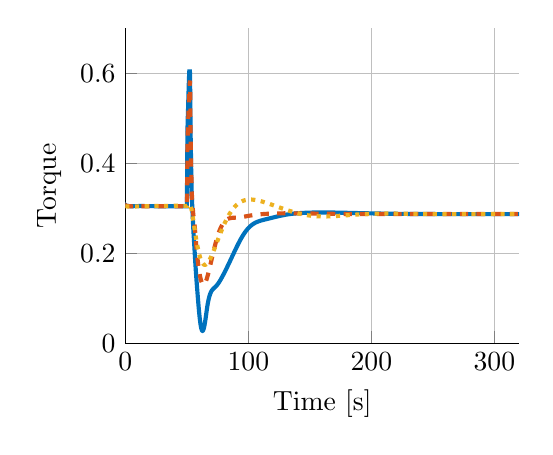
\begin{tikzpicture}

\begin{axis}[%
width=5cm,
height=4cm,
at={(0\linewidth,0\linewidth)},
scale only axis,
xmin=0,
xmax=320,
xlabel={Time [s]},
xmajorgrids,
ymin=0,
ymax=0.7,
ylabel={Torque},
ymajorgrids,
axis background/.style={fill=white},
% title style={font=\bfseries},
% title={Normalized Torque Setting},
axis x line*=bottom,
axis y line*=left
]
\addplot [color=mycolor1,solid,line width=1.5pt,forget plot]
  table[row sep=crcr]{%
0	0.304831074\\
0.25	0.30665978\\
0.5	0.30590085\\
0.75	0.30562405\\
1	0.30565309\\
1.25	0.30547614\\
1.5	0.30528095\\
1.75	0.30515676\\
2	0.30504243\\
2.25	0.304928319\\
2.5	0.304830357\\
2.75	0.30474751\\
3	0.304675987\\
3.25	0.304616093\\
3.5	0.304567996\\
3.75	0.304530753\\
4	0.304503022\\
4.25	0.304483048\\
4.5	0.304468969\\
4.75	0.304459287\\
5	0.304453134\\
5.25	0.304450003\\
5.5	0.304449628\\
5.75	0.304452033\\
6	0.304457403\\
6.25	0.304465922\\
6.5	0.304477601\\
6.75	0.304492142\\
7	0.304508918\\
7.25	0.304527087\\
7.5	0.304545747\\
7.75	0.30456407\\
8	0.304581427\\
8.25	0.304597482\\
8.5	0.304612217\\
8.75	0.30462589\\
9	0.304638928\\
9.25	0.304651779\\
9.5	0.304664765\\
9.75	0.304677988\\
10	0.304691287\\
10.25	0.304704276\\
10.5	0.304716429\\
10.75	0.304727207\\
11	0.304736188\\
11.25	0.30474316\\
11.5	0.304748177\\
11.75	0.304751534\\
12	0.304753694\\
12.25	0.304755174\\
12.5	0.304756414\\
12.75	0.304757681\\
13	0.30475901\\
13.25	0.30476021\\
13.5	0.304760922\\
13.75	0.30476073\\
14	0.304759267\\
14.25	0.304756327\\
14.5	0.304751915\\
14.75	0.30474626\\
15	0.304739763\\
15.25	0.304732898\\
15.5	0.304726109\\
15.75	0.304719702\\
16	0.304713781\\
16.25	0.304708235\\
16.5	0.304702777\\
16.75	0.304697029\\
17	0.30469063\\
17.25	0.304683333\\
17.5	0.304675073\\
17.75	0.304665996\\
18	0.304656418\\
18.25	0.304646755\\
18.5	0.304637419\\
18.75	0.304628722\\
19	0.304620796\\
19.25	0.304613572\\
19.5	0.304606803\\
19.75	0.304600131\\
20	0.304593187\\
20.25	0.304585688\\
20.5	0.304577512\\
20.75	0.304568734\\
21	0.304559605\\
21.25	0.304550493\\
21.5	0.304541785\\
21.75	0.304533794\\
22	0.304526677\\
22.25	0.304520397\\
22.5	0.304514737\\
22.75	0.304509357\\
23	0.304503883\\
23.25	0.304498007\\
23.5	0.304491565\\
23.75	0.30448458\\
24	0.30447726\\
24.25	0.30446994\\
24.5	0.304462995\\
24.75	0.304456747\\
25	0.304451375\\
25.25	0.304446874\\
25.5	0.304443053\\
25.75	0.304439586\\
26	0.304436097\\
26.25	0.304432258\\
26.5	0.304427872\\
26.75	0.304422928\\
27	0.304417601\\
27.25	0.304412209\\
27.5	0.304407124\\
27.75	0.304402683\\
28	0.304399091\\
28.25	0.30439637\\
28.5	0.30439435\\
28.75	0.304392716\\
29	0.304391086\\
29.25	0.304389111\\
29.5	0.304386568\\
29.75	0.304383418\\
30	0.304379815\\
30.25	0.304376067\\
30.5	0.304372557\\
30.75	0.304369637\\
31	0.30436754\\
31.25	0.304366312\\
31.5	0.304365801\\
31.75	0.304365694\\
32	0.304365598\\
32.25	0.304365143\\
32.5	0.304364077\\
32.75	0.304362337\\
33	0.304360064\\
33.25	0.304357567\\
33.5	0.304355243\\
33.75	0.304353469\\
34	0.304352507\\
34.25	0.304352425\\
34.5	0.304353082\\
34.75	0.30435416\\
35	0.304355248\\
35.25	0.304355947\\
35.5	0.304355978\\
35.75	0.304355255\\
36	0.304353912\\
36.25	0.304352267\\
36.5	0.30435074\\
36.75	0.304349742\\
37	0.304349564\\
37.25	0.304350296\\
37.5	0.304351802\\
37.75	0.304353751\\
38	0.304355704\\
38.25	0.304357226\\
38.5	0.304358006\\
38.75	0.304357939\\
39	0.304357157\\
39.25	0.304355997\\
39.5	0.304354913\\
39.75	0.304354356\\
40	0.304354653\\
40.25	0.304355914\\
40.5	0.304358003\\
40.75	0.304360563\\
41	0.304363117\\
41.25	0.304365186\\
41.5	0.30436642\\
41.75	0.304366697\\
42	0.304366153\\
42.25	0.304365156\\
42.5	0.304364208\\
42.75	0.304363811\\
43	0.304364333\\
43.25	0.304365904\\
43.5	0.304368376\\
43.75	0.30437136\\
44	0.304374322\\
44.25	0.304376726\\
44.5	0.30437818\\
44.75	0.304378543\\
45	0.304377967\\
45.25	0.304376863\\
45.5	0.304375798\\
45.75	0.304375339\\
46	0.304375903\\
46.25	0.304377638\\
46.5	0.304380377\\
46.75	0.304383675\\
47	0.304386927\\
47.25	0.304389525\\
47.5	0.304391024\\
47.75	0.304391267\\
48	0.304390434\\
48.25	0.304389\\
48.5	0.304387617\\
48.75	0.304386935\\
49	0.304387429\\
49.25	0.30438926\\
49.5	0.304392228\\
49.75	0.304395814\\
50	0.304399313\\
50.25	0.3726148\\
50.5	0.472673\\
50.75	0.500789\\
51	0.520824\\
51.25	0.544824\\
51.5	0.568657\\
51.75	0.588946\\
52	0.604\\
52.25	0.604\\
52.5	0.604\\
52.75	0.557336\\
53	0.474781\\
53.25	0.433629\\
53.5	0.3906805\\
53.75	0.3545439\\
54	0.330705\\
54.25	0.31342796\\
54.5	0.29890661\\
54.75	0.2832353\\
55	0.2678304\\
55.25	0.2541441\\
55.5	0.2419374\\
55.75	0.2305571\\
56	0.2195289\\
56.25	0.207966\\
56.5	0.196075\\
56.75	0.184581\\
57	0.173632\\
57.25	0.163105\\
57.5	0.153024\\
57.75	0.143495\\
58	0.134445\\
58.25	0.125621\\
58.5	0.116863\\
58.75	0.108186\\
59	0.099649\\
59.25	0.091303\\
59.5	0.083216\\
59.75	0.075468\\
60	0.068134\\
60.25	0.061278\\
60.5	0.054953\\
60.75	0.04921\\
61	0.044088\\
61.25	0.03962\\
61.5	0.035826\\
61.75	0.032722\\
62	0.030319\\
62.25	0.028618\\
62.5	0.027615\\
62.75	0.027302\\
63	0.027661\\
63.25	0.028668\\
63.5	0.030292\\
63.75	0.032495\\
64	0.03523\\
64.25	0.038446\\
64.5	0.042088\\
64.75	0.046101\\
65	0.05043\\
65.25	0.055024\\
65.5	0.059828\\
65.75	0.064776\\
66	0.069773\\
66.25	0.074692\\
66.5	0.079392\\
66.75	0.083771\\
67	0.087791\\
67.25	0.091463\\
67.5	0.094815\\
67.75	0.097879\\
68	0.100681\\
68.25	0.103241\\
68.5	0.105574\\
68.75	0.107693\\
69	0.109612\\
69.25	0.111343\\
69.5	0.1129\\
69.75	0.114296\\
70	0.115547\\
70.25	0.116669\\
70.5	0.117678\\
70.75	0.118589\\
71	0.119418\\
71.25	0.120181\\
71.5	0.120893\\
71.75	0.121566\\
72	0.122213\\
72.25	0.122845\\
72.5	0.123472\\
72.75	0.124104\\
73	0.124748\\
73.25	0.125409\\
73.5	0.126093\\
73.75	0.126805\\
74	0.127547\\
74.25	0.128322\\
74.5	0.129131\\
74.75	0.129975\\
75	0.130854\\
75.25	0.131768\\
75.5	0.132715\\
75.75	0.133696\\
76	0.134709\\
76.25	0.135752\\
76.5	0.136823\\
76.75	0.137922\\
77	0.139046\\
77.25	0.140193\\
77.5	0.141363\\
77.75	0.142553\\
78	0.143762\\
78.25	0.144988\\
78.5	0.146231\\
78.75	0.147488\\
79	0.14876\\
79.25	0.150044\\
79.5	0.151341\\
79.75	0.152648\\
80	0.153966\\
80.25	0.155295\\
80.5	0.156632\\
80.75	0.157978\\
81	0.159333\\
81.25	0.160695\\
81.5	0.162065\\
81.75	0.163443\\
82	0.164827\\
82.25	0.166219\\
82.5	0.167616\\
82.75	0.16902\\
83	0.17043\\
83.25	0.171846\\
83.5	0.173267\\
83.75	0.174694\\
84	0.176125\\
84.25	0.177561\\
84.5	0.179001\\
84.75	0.180445\\
85	0.181892\\
85.25	0.183343\\
85.5	0.184796\\
85.75	0.186252\\
86	0.187709\\
86.25	0.189168\\
86.5	0.190628\\
86.75	0.192089\\
87	0.193549\\
87.25	0.195009\\
87.5	0.196468\\
87.75	0.197925\\
88	0.19938\\
88.25	0.200832\\
88.5	0.20228\\
88.75	0.203725\\
89	0.2051655\\
89.25	0.2066006\\
89.5	0.20803\\
89.75	0.2094529\\
90	0.2108689\\
90.25	0.2122773\\
90.5	0.2136774\\
90.75	0.2150687\\
91	0.2164505\\
91.25	0.2178222\\
91.5	0.2191833\\
91.75	0.220533\\
92	0.2218709\\
92.25	0.2231964\\
92.5	0.2245088\\
92.75	0.2258076\\
93	0.2270923\\
93.25	0.2283623\\
93.5	0.229617\\
93.75	0.2308561\\
94	0.232079\\
94.25	0.2332852\\
94.5	0.2344743\\
94.75	0.2356458\\
95	0.2367994\\
95.25	0.2379346\\
95.5	0.239051\\
95.75	0.2401485\\
96	0.2412265\\
96.25	0.2422849\\
96.5	0.2433234\\
96.75	0.2443417\\
97	0.2453396\\
97.25	0.246317\\
97.5	0.2472736\\
97.75	0.2482094\\
98	0.2491243\\
98.25	0.2500181\\
98.5	0.2508909\\
98.75	0.2517427\\
99	0.2525734\\
99.25	0.253383\\
99.5	0.2541718\\
99.75	0.2549397\\
100	0.2556869\\
100.25	0.2564135\\
100.5	0.2571197\\
100.75	0.2578057\\
101	0.2584718\\
101.25	0.2591181\\
101.5	0.2597449\\
101.75	0.2603526\\
102	0.2609415\\
102.25	0.2615118\\
102.5	0.2620639\\
102.75	0.2625982\\
103	0.2631151\\
103.25	0.2636149\\
103.5	0.2640981\\
103.75	0.2645651\\
104	0.2650163\\
104.25	0.2654522\\
104.5	0.2658731\\
104.75	0.2662797\\
105	0.2666722\\
105.25	0.2670513\\
105.5	0.2674173\\
105.75	0.2677708\\
106	0.2681122\\
106.25	0.268442\\
106.5	0.2687607\\
106.75	0.2690687\\
107	0.2693666\\
107.25	0.2696547\\
107.5	0.2699336\\
107.75	0.2702038\\
108	0.2704655\\
108.25	0.2707194\\
108.5	0.2709658\\
108.75	0.2712052\\
109	0.271438\\
109.25	0.2716646\\
109.5	0.2718853\\
109.75	0.2721007\\
110	0.2723109\\
110.25	0.2725165\\
110.5	0.2727177\\
110.75	0.2729149\\
111	0.2731085\\
111.25	0.2732986\\
111.5	0.2734857\\
111.75	0.2736699\\
112	0.2738516\\
112.25	0.2740311\\
112.5	0.2742085\\
112.75	0.274384\\
113	0.274558\\
113.25	0.2747306\\
113.5	0.2749019\\
113.75	0.2750723\\
114	0.2752417\\
114.25	0.2754104\\
114.5	0.2755785\\
114.75	0.2757461\\
115	0.2759133\\
115.25	0.2760803\\
115.5	0.2762471\\
115.75	0.2764138\\
116	0.2765804\\
116.25	0.2767471\\
116.5	0.2769138\\
116.75	0.2770806\\
117	0.2772476\\
117.25	0.2774147\\
117.5	0.277582\\
117.75	0.2777494\\
118	0.277917\\
118.25	0.2780848\\
118.5	0.2782527\\
118.75	0.2784207\\
119	0.2785889\\
119.25	0.2787571\\
119.5	0.2789253\\
119.75	0.2790935\\
120	0.2792617\\
120.25	0.2794298\\
120.5	0.2795977\\
120.75	0.2797655\\
121	0.2799329\\
121.25	0.2801001\\
121.5	0.2802669\\
121.75	0.2804333\\
122	0.2805992\\
122.25	0.2807645\\
122.5	0.2809292\\
122.75	0.2810933\\
123	0.2812566\\
123.25	0.2814191\\
123.5	0.2815808\\
123.75	0.2817416\\
124	0.2819013\\
124.25	0.2820601\\
124.5	0.2822177\\
124.75	0.2823742\\
125	0.2825295\\
125.25	0.2826835\\
125.5	0.2828362\\
125.75	0.2829876\\
126	0.2831376\\
126.25	0.2832861\\
126.5	0.2834331\\
126.75	0.2835786\\
127	0.2837225\\
127.25	0.2838648\\
127.5	0.2840054\\
127.75	0.2841444\\
128	0.2842816\\
128.25	0.2844171\\
128.5	0.2845509\\
128.75	0.2846829\\
129	0.284813\\
129.25	0.2849414\\
129.5	0.2850679\\
129.75	0.2851925\\
130	0.2853153\\
130.25	0.2854361\\
130.5	0.2855551\\
130.75	0.2856722\\
131	0.2857874\\
131.25	0.2859007\\
131.5	0.2860121\\
131.75	0.2861216\\
132	0.2862292\\
132.25	0.2863349\\
132.5	0.2864387\\
132.75	0.2865407\\
133	0.2866407\\
133.25	0.286739\\
133.5	0.2868353\\
133.75	0.2869298\\
134	0.2870225\\
134.25	0.2871134\\
134.5	0.2872026\\
134.75	0.2872899\\
135	0.2873755\\
135.25	0.2874594\\
135.5	0.2875415\\
135.75	0.287622\\
136	0.2877008\\
136.25	0.2877779\\
136.5	0.2878534\\
136.75	0.2879273\\
137	0.2879996\\
137.25	0.2880704\\
137.5	0.2881397\\
137.75	0.2882074\\
138	0.2882737\\
138.25	0.2883385\\
138.5	0.2884018\\
138.75	0.2884638\\
139	0.2885244\\
139.25	0.2885836\\
139.5	0.2886415\\
139.75	0.2886981\\
140	0.2887534\\
140.25	0.2888074\\
140.5	0.2888602\\
140.75	0.2889118\\
141	0.2889622\\
141.25	0.2890114\\
141.5	0.2890595\\
141.75	0.2891065\\
142	0.2891523\\
142.25	0.2891971\\
142.5	0.2892409\\
142.75	0.2892836\\
143	0.2893253\\
143.25	0.289366\\
143.5	0.2894057\\
143.75	0.2894445\\
144	0.2894823\\
144.25	0.2895192\\
144.5	0.2895553\\
144.75	0.2895904\\
145	0.2896247\\
145.25	0.2896581\\
145.5	0.2896907\\
145.75	0.2897225\\
146	0.2897535\\
146.25	0.2897837\\
146.5	0.2898132\\
146.75	0.2898419\\
147	0.2898698\\
147.25	0.289897\\
147.5	0.2899235\\
147.75	0.2899493\\
148	0.2899744\\
148.25	0.2899988\\
148.5	0.2900225\\
148.75	0.2900456\\
149	0.2900681\\
149.25	0.2900899\\
149.5	0.290111\\
149.75	0.2901316\\
150	0.2901515\\
150.25	0.2901708\\
150.5	0.2901896\\
150.75	0.2902077\\
151	0.2902253\\
151.25	0.2902423\\
151.5	0.2902588\\
151.75	0.2902747\\
152	0.29029\\
152.25	0.2903048\\
152.5	0.2903191\\
152.75	0.2903328\\
153	0.2903461\\
153.25	0.2903588\\
153.5	0.290371\\
153.75	0.2903826\\
154	0.2903938\\
154.25	0.2904045\\
154.5	0.2904148\\
154.75	0.2904245\\
155	0.2904338\\
155.25	0.2904425\\
155.5	0.2904509\\
155.75	0.2904587\\
156	0.2904661\\
156.25	0.2904731\\
156.5	0.2904796\\
156.75	0.2904857\\
157	0.2904913\\
157.25	0.2904965\\
157.5	0.2905012\\
157.75	0.2905056\\
158	0.2905095\\
158.25	0.290513\\
158.5	0.2905161\\
158.75	0.2905188\\
159	0.2905211\\
159.25	0.290523\\
159.5	0.2905245\\
159.75	0.2905257\\
160	0.2905264\\
160.25	0.2905268\\
160.5	0.2905268\\
160.75	0.2905264\\
161	0.2905256\\
161.25	0.2905245\\
161.5	0.2905231\\
161.75	0.2905213\\
162	0.2905191\\
162.25	0.2905166\\
162.5	0.2905138\\
162.75	0.2905106\\
163	0.2905071\\
163.25	0.2905033\\
163.5	0.2904992\\
163.75	0.2904947\\
164	0.29049\\
164.25	0.2904849\\
164.5	0.2904796\\
164.75	0.2904739\\
165	0.2904679\\
165.25	0.2904617\\
165.5	0.2904552\\
165.75	0.2904484\\
166	0.2904413\\
166.25	0.290434\\
166.5	0.2904264\\
166.75	0.2904185\\
167	0.2904104\\
167.25	0.290402\\
167.5	0.2903934\\
167.75	0.2903846\\
168	0.2903755\\
168.25	0.2903662\\
168.5	0.2903566\\
168.75	0.2903469\\
169	0.2903369\\
169.25	0.2903267\\
169.5	0.2903162\\
169.75	0.2903056\\
170	0.2902948\\
170.25	0.2902838\\
170.5	0.2902726\\
170.75	0.2902612\\
171	0.2902496\\
171.25	0.2902378\\
171.5	0.2902259\\
171.75	0.2902138\\
172	0.2902015\\
172.25	0.290189\\
172.5	0.2901764\\
172.75	0.2901637\\
173	0.2901508\\
173.25	0.2901377\\
173.5	0.2901245\\
173.75	0.2901112\\
174	0.2900977\\
174.25	0.2900841\\
174.5	0.2900703\\
174.75	0.2900564\\
175	0.2900424\\
175.25	0.2900283\\
175.5	0.2900141\\
175.75	0.2899998\\
176	0.2899853\\
176.25	0.2899708\\
176.5	0.2899561\\
176.75	0.2899414\\
177	0.2899265\\
177.25	0.2899116\\
177.5	0.2898965\\
177.75	0.2898814\\
178	0.2898662\\
178.25	0.2898509\\
178.5	0.2898356\\
178.75	0.2898202\\
179	0.2898047\\
179.25	0.2897891\\
179.5	0.2897735\\
179.75	0.2897578\\
180	0.289742\\
180.25	0.2897262\\
180.5	0.2897103\\
180.75	0.2896944\\
181	0.2896785\\
181.25	0.2896625\\
181.5	0.2896464\\
181.75	0.2896303\\
182	0.2896142\\
182.25	0.289598\\
182.5	0.2895818\\
182.75	0.2895655\\
183	0.2895493\\
183.25	0.289533\\
183.5	0.2895167\\
183.75	0.2895003\\
184	0.2894839\\
184.25	0.2894676\\
184.5	0.2894511\\
184.75	0.2894347\\
185	0.2894183\\
185.25	0.2894019\\
185.5	0.2893854\\
185.75	0.289369\\
186	0.2893525\\
186.25	0.289336\\
186.5	0.2893196\\
186.75	0.2893031\\
187	0.2892866\\
187.25	0.2892702\\
187.5	0.2892537\\
187.75	0.2892373\\
188	0.2892208\\
188.25	0.2892044\\
188.5	0.289188\\
188.75	0.2891716\\
189	0.2891552\\
189.25	0.2891388\\
189.5	0.2891225\\
189.75	0.2891061\\
190	0.2890898\\
190.25	0.2890735\\
190.5	0.2890573\\
190.75	0.289041\\
191	0.2890248\\
191.25	0.2890086\\
191.5	0.2889925\\
191.75	0.2889764\\
192	0.2889603\\
192.25	0.2889442\\
192.5	0.2889282\\
192.75	0.2889122\\
193	0.2888962\\
193.25	0.2888803\\
193.5	0.2888644\\
193.75	0.2888486\\
194	0.2888328\\
194.25	0.2888171\\
194.5	0.2888014\\
194.75	0.2887857\\
195	0.2887701\\
195.25	0.2887545\\
195.5	0.288739\\
195.75	0.2887235\\
196	0.2887081\\
196.25	0.2886927\\
196.5	0.2886774\\
196.75	0.2886621\\
197	0.2886469\\
197.25	0.2886317\\
197.5	0.2886166\\
197.75	0.2886016\\
198	0.2885866\\
198.25	0.2885716\\
198.5	0.2885568\\
198.75	0.2885419\\
199	0.2885272\\
199.25	0.2885125\\
199.5	0.2884978\\
199.75	0.2884832\\
200	0.2884687\\
200.25	0.2884543\\
200.5	0.2884399\\
200.75	0.2884255\\
201	0.2884113\\
201.25	0.2883971\\
201.5	0.2883829\\
201.75	0.2883689\\
202	0.2883549\\
202.25	0.2883409\\
202.5	0.2883271\\
202.75	0.2883133\\
203	0.2882995\\
203.25	0.2882859\\
203.5	0.2882723\\
203.75	0.2882588\\
204	0.2882453\\
204.25	0.288232\\
204.5	0.2882186\\
204.75	0.2882054\\
205	0.2881922\\
205.25	0.2881792\\
205.5	0.2881661\\
205.75	0.2881532\\
206	0.2881403\\
206.25	0.2881275\\
206.5	0.2881148\\
206.75	0.2881022\\
207	0.2880896\\
207.25	0.2880771\\
207.5	0.2880647\\
207.75	0.2880523\\
208	0.28804\\
208.25	0.2880278\\
208.5	0.2880157\\
208.75	0.2880037\\
209	0.2879917\\
209.25	0.2879798\\
209.5	0.287968\\
209.75	0.2879562\\
210	0.2879446\\
210.25	0.287933\\
210.5	0.2879215\\
210.75	0.28791\\
211	0.2878987\\
211.25	0.2878874\\
211.5	0.2878762\\
211.75	0.2878651\\
212	0.287854\\
212.25	0.287843\\
212.5	0.2878321\\
212.75	0.2878213\\
213	0.2878106\\
213.25	0.2877999\\
213.5	0.2877893\\
213.75	0.2877788\\
214	0.2877684\\
214.25	0.287758\\
214.5	0.2877478\\
214.75	0.2877376\\
215	0.2877274\\
215.25	0.2877174\\
215.5	0.2877074\\
215.75	0.2876975\\
216	0.2876877\\
216.25	0.287678\\
216.5	0.2876683\\
216.75	0.2876587\\
217	0.2876492\\
217.25	0.2876398\\
217.5	0.2876304\\
217.75	0.2876211\\
218	0.2876119\\
218.25	0.2876028\\
218.5	0.2875937\\
218.75	0.2875848\\
219	0.2875759\\
219.25	0.287567\\
219.5	0.2875583\\
219.75	0.2875496\\
220	0.287541\\
220.25	0.2875324\\
220.5	0.287524\\
220.75	0.2875156\\
221	0.2875073\\
221.25	0.287499\\
221.5	0.2874909\\
221.75	0.2874828\\
222	0.2874747\\
222.25	0.2874668\\
222.5	0.2874589\\
222.75	0.2874511\\
223	0.2874434\\
223.25	0.2874357\\
223.5	0.2874281\\
223.75	0.2874206\\
224	0.2874131\\
224.25	0.2874057\\
224.5	0.2873984\\
224.75	0.2873912\\
225	0.287384\\
225.25	0.2873769\\
225.5	0.2873699\\
225.75	0.2873629\\
226	0.287356\\
226.25	0.2873491\\
226.5	0.2873424\\
226.75	0.2873357\\
227	0.287329\\
227.25	0.2873225\\
227.5	0.287316\\
227.75	0.2873095\\
228	0.2873032\\
228.25	0.2872969\\
228.5	0.2872906\\
228.75	0.2872844\\
229	0.2872783\\
229.25	0.2872723\\
229.5	0.2872663\\
229.75	0.2872604\\
230	0.2872545\\
230.25	0.2872487\\
230.5	0.287243\\
230.75	0.2872373\\
231	0.2872317\\
231.25	0.2872261\\
231.5	0.2872207\\
231.75	0.2872152\\
232	0.2872099\\
232.25	0.2872045\\
232.5	0.2871993\\
232.75	0.2871941\\
233	0.287189\\
233.25	0.2871839\\
233.5	0.2871789\\
233.75	0.2871739\\
234	0.287169\\
234.25	0.2871642\\
234.5	0.2871594\\
234.75	0.2871546\\
235	0.28715\\
235.25	0.2871453\\
235.5	0.2871408\\
235.75	0.2871363\\
236	0.2871318\\
236.25	0.2871274\\
236.5	0.287123\\
236.75	0.2871187\\
237	0.2871145\\
237.25	0.2871103\\
237.5	0.2871062\\
237.75	0.2871021\\
238	0.287098\\
238.25	0.2870941\\
238.5	0.2870901\\
238.75	0.2870862\\
239	0.2870824\\
239.25	0.2870786\\
239.5	0.2870749\\
239.75	0.2870712\\
240	0.2870675\\
240.25	0.2870639\\
240.5	0.2870604\\
240.75	0.2870569\\
241	0.2870534\\
241.25	0.28705\\
241.5	0.2870467\\
241.75	0.2870434\\
242	0.2870401\\
242.25	0.2870369\\
242.5	0.2870337\\
242.75	0.2870306\\
243	0.2870275\\
243.25	0.2870244\\
243.5	0.2870214\\
243.75	0.2870185\\
244	0.2870155\\
244.25	0.2870127\\
244.5	0.2870098\\
244.75	0.287007\\
245	0.2870043\\
245.25	0.2870016\\
245.5	0.2869989\\
245.75	0.2869963\\
246	0.2869937\\
246.25	0.2869911\\
246.5	0.2869886\\
246.75	0.2869861\\
247	0.2869837\\
247.25	0.2869813\\
247.5	0.2869789\\
247.75	0.2869766\\
248	0.2869743\\
248.25	0.2869721\\
248.5	0.2869699\\
248.75	0.2869677\\
249	0.2869656\\
249.25	0.2869635\\
249.5	0.2869614\\
249.75	0.2869593\\
250	0.2869573\\
250.25	0.2869554\\
250.5	0.2869534\\
250.75	0.2869515\\
251	0.2869497\\
251.25	0.2869478\\
251.5	0.286946\\
251.75	0.2869443\\
252	0.2869425\\
252.25	0.2869408\\
252.5	0.2869391\\
252.75	0.2869375\\
253	0.2869359\\
253.25	0.2869343\\
253.5	0.2869327\\
253.75	0.2869312\\
254	0.2869297\\
254.25	0.2869282\\
254.5	0.2869268\\
254.75	0.2869254\\
255	0.286924\\
255.25	0.2869227\\
255.5	0.2869213\\
255.75	0.28692\\
256	0.2869188\\
256.25	0.2869175\\
256.5	0.2869163\\
256.75	0.2869151\\
257	0.2869139\\
257.25	0.2869128\\
257.5	0.2869117\\
257.75	0.2869106\\
258	0.2869095\\
258.25	0.2869084\\
258.5	0.2869074\\
258.75	0.2869064\\
259	0.2869054\\
259.25	0.2869045\\
259.5	0.2869036\\
259.75	0.2869027\\
260	0.2869018\\
260.25	0.2869009\\
260.5	0.2869001\\
260.75	0.2868993\\
261	0.2868985\\
261.25	0.2868977\\
261.5	0.2868969\\
261.75	0.2868962\\
262	0.2868955\\
262.25	0.2868948\\
262.5	0.2868941\\
262.75	0.2868935\\
263	0.2868928\\
263.25	0.2868922\\
263.5	0.2868916\\
263.75	0.286891\\
264	0.2868905\\
264.25	0.2868899\\
264.5	0.2868894\\
264.75	0.2868889\\
265	0.2868884\\
265.25	0.2868879\\
265.5	0.2868875\\
265.75	0.286887\\
266	0.2868866\\
266.25	0.2868862\\
266.5	0.2868858\\
266.75	0.2868854\\
267	0.2868851\\
267.25	0.2868847\\
267.5	0.2868844\\
267.75	0.2868841\\
268	0.2868838\\
268.25	0.2868835\\
268.5	0.2868832\\
268.75	0.286883\\
269	0.2868827\\
269.25	0.2868825\\
269.5	0.2868823\\
269.75	0.2868821\\
270	0.2868819\\
270.25	0.2868817\\
270.5	0.2868816\\
270.75	0.2868814\\
271	0.2868813\\
271.25	0.2868812\\
271.5	0.2868811\\
271.75	0.286881\\
272	0.2868809\\
272.25	0.2868808\\
272.5	0.2868807\\
272.75	0.2868807\\
273	0.2868806\\
273.25	0.2868806\\
273.5	0.2868806\\
273.75	0.2868805\\
274	0.2868805\\
274.25	0.2868806\\
274.5	0.2868806\\
274.75	0.2868806\\
275	0.2868806\\
275.25	0.2868807\\
275.5	0.2868807\\
275.75	0.2868808\\
276	0.2868809\\
276.25	0.286881\\
276.5	0.2868811\\
276.75	0.2868812\\
277	0.2868813\\
277.25	0.2868814\\
277.5	0.2868815\\
277.75	0.2868816\\
278	0.2868818\\
278.25	0.2868819\\
278.5	0.2868821\\
278.75	0.2868822\\
279	0.2868824\\
279.25	0.2868826\\
279.5	0.2868828\\
279.75	0.286883\\
280	0.2868832\\
280.25	0.2868834\\
280.5	0.2868836\\
280.75	0.2868838\\
281	0.286884\\
281.25	0.2868842\\
281.5	0.2868845\\
281.75	0.2868847\\
282	0.2868849\\
282.25	0.2868852\\
282.5	0.2868855\\
282.75	0.2868857\\
283	0.286886\\
283.25	0.2868863\\
283.5	0.2868865\\
283.75	0.2868868\\
284	0.2868871\\
284.25	0.2868874\\
284.5	0.2868877\\
284.75	0.286888\\
285	0.2868883\\
285.25	0.2868886\\
285.5	0.2868889\\
285.75	0.2868892\\
286	0.2868895\\
286.25	0.2868899\\
286.5	0.2868902\\
286.75	0.2868905\\
287	0.2868909\\
287.25	0.2868912\\
287.5	0.2868915\\
287.75	0.2868919\\
288	0.2868922\\
288.25	0.2868926\\
288.5	0.2868929\\
288.75	0.2868933\\
289	0.2868936\\
289.25	0.286894\\
289.5	0.2868944\\
289.75	0.2868947\\
290	0.2868951\\
290.25	0.2868955\\
290.5	0.2868958\\
290.75	0.2868962\\
291	0.2868966\\
291.25	0.286897\\
291.5	0.2868974\\
291.75	0.2868977\\
292	0.2868981\\
292.25	0.2868985\\
292.5	0.2868989\\
292.75	0.2868993\\
293	0.2868997\\
293.25	0.2869001\\
293.5	0.2869005\\
293.75	0.2869009\\
294	0.2869013\\
294.25	0.2869017\\
294.5	0.286902\\
294.75	0.2869024\\
295	0.2869028\\
295.25	0.2869032\\
295.5	0.2869037\\
295.75	0.2869041\\
296	0.2869045\\
296.25	0.2869049\\
296.5	0.2869053\\
296.75	0.2869057\\
297	0.2869061\\
297.25	0.2869065\\
297.5	0.2869069\\
297.75	0.2869073\\
298	0.2869077\\
298.25	0.2869081\\
298.5	0.2869085\\
298.75	0.2869089\\
299	0.2869093\\
299.25	0.2869097\\
299.5	0.2869101\\
299.75	0.2869105\\
300	0.286911\\
300.25	0.2869114\\
300.5	0.2869118\\
300.75	0.2869122\\
301	0.2869126\\
301.25	0.286913\\
301.5	0.2869134\\
301.75	0.2869138\\
302	0.2869142\\
302.25	0.2869146\\
302.5	0.286915\\
302.75	0.2869154\\
303	0.2869158\\
303.25	0.2869162\\
303.5	0.2869166\\
303.75	0.286917\\
304	0.2869174\\
304.25	0.2869178\\
304.5	0.2869182\\
304.75	0.2869186\\
305	0.286919\\
305.25	0.2869194\\
305.5	0.2869198\\
305.75	0.2869202\\
306	0.2869206\\
306.25	0.286921\\
306.5	0.2869214\\
306.75	0.2869217\\
307	0.2869221\\
307.25	0.2869225\\
307.5	0.2869229\\
307.75	0.2869233\\
308	0.2869237\\
308.25	0.286924\\
308.5	0.2869244\\
308.75	0.2869248\\
309	0.2869252\\
309.25	0.2869256\\
309.5	0.2869259\\
309.75	0.2869263\\
310	0.2869267\\
310.25	0.286927\\
310.5	0.2869274\\
310.75	0.2869278\\
311	0.2869281\\
311.25	0.2869285\\
311.5	0.2869289\\
311.75	0.2869292\\
312	0.2869296\\
312.25	0.28693\\
312.5	0.2869303\\
312.75	0.2869307\\
313	0.286931\\
313.25	0.2869314\\
313.5	0.2869317\\
313.75	0.2869321\\
314	0.2869324\\
314.25	0.2869328\\
314.5	0.2869331\\
314.75	0.2869334\\
315	0.2869338\\
315.25	0.2869341\\
315.5	0.2869345\\
315.75	0.2869348\\
316	0.2869351\\
316.25	0.2869355\\
316.5	0.2869358\\
316.75	0.2869361\\
317	0.2869364\\
317.25	0.2869368\\
317.5	0.2869371\\
317.75	0.2869374\\
318	0.2869377\\
318.25	0.286938\\
318.5	0.2869383\\
318.75	0.2869387\\
319	0.286939\\
319.25	0.2869393\\
319.5	0.2869396\\
319.75	0.2869399\\
320	0.2869402\\
320.25	0.2869405\\
320.5	0.2869408\\
320.75	0.2869411\\
321	0.2869414\\
321.25	0.2869417\\
321.5	0.286942\\
321.75	0.2869423\\
322	0.2869426\\
322.25	0.2869428\\
322.5	0.2869431\\
322.75	0.2869434\\
323	0.2869437\\
323.25	0.286944\\
323.5	0.2869442\\
323.75	0.2869445\\
324	0.2869448\\
324.25	0.2869451\\
324.5	0.2869453\\
324.75	0.2869456\\
325	0.2869459\\
325.25	0.2869461\\
325.5	0.2869464\\
325.75	0.2869466\\
326	0.2869469\\
326.25	0.2869472\\
326.5	0.2869474\\
326.75	0.2869477\\
327	0.2869479\\
327.25	0.2869482\\
327.5	0.2869484\\
327.75	0.2869486\\
328	0.2869489\\
328.25	0.2869491\\
328.5	0.2869494\\
328.75	0.2869496\\
329	0.2869498\\
329.25	0.2869501\\
329.5	0.2869503\\
329.75	0.2869505\\
330	0.2869508\\
330.25	0.286951\\
330.5	0.2869512\\
330.75	0.2869514\\
331	0.2869516\\
331.25	0.2869519\\
331.5	0.2869521\\
331.75	0.2869523\\
332	0.2869525\\
332.25	0.2869527\\
332.5	0.2869529\\
332.75	0.2869531\\
333	0.2869533\\
333.25	0.2869535\\
333.5	0.2869537\\
333.75	0.2869539\\
334	0.2869541\\
334.25	0.2869543\\
334.5	0.2869545\\
334.75	0.2869547\\
335	0.2869549\\
335.25	0.2869551\\
335.5	0.2869553\\
335.75	0.2869555\\
336	0.2869557\\
336.25	0.2869558\\
336.5	0.286956\\
336.75	0.2869562\\
337	0.2869564\\
337.25	0.2869565\\
337.5	0.2869567\\
337.75	0.2869569\\
338	0.2869571\\
338.25	0.2869572\\
338.5	0.2869574\\
338.75	0.2869576\\
339	0.2869577\\
339.25	0.2869579\\
339.5	0.286958\\
339.75	0.2869582\\
340	0.2869584\\
340.25	0.2869585\\
340.5	0.2869587\\
340.75	0.2869588\\
341	0.286959\\
341.25	0.2869591\\
341.5	0.2869593\\
341.75	0.2869594\\
342	0.2869596\\
342.25	0.2869597\\
342.5	0.2869598\\
342.75	0.28696\\
343	0.2869601\\
343.25	0.2869603\\
343.5	0.2869604\\
343.75	0.2869605\\
344	0.2869607\\
344.25	0.2869608\\
344.5	0.2869609\\
344.75	0.286961\\
345	0.2869612\\
345.25	0.2869613\\
345.5	0.2869614\\
345.75	0.2869615\\
346	0.2869617\\
346.25	0.2869618\\
346.5	0.2869619\\
346.75	0.286962\\
347	0.2869621\\
347.25	0.2869622\\
347.5	0.2869624\\
347.75	0.2869625\\
348	0.2869626\\
348.25	0.2869627\\
348.5	0.2869628\\
348.75	0.2869629\\
349	0.286963\\
349.25	0.2869631\\
349.5	0.2869632\\
349.75	0.2869633\\
350	0.2869634\\
350.25	0.2869635\\
350.5	0.2869636\\
350.75	0.2869637\\
351	0.2869638\\
351.25	0.2869639\\
351.5	0.286964\\
351.75	0.2869641\\
352	0.2869642\\
352.25	0.2869642\\
352.5	0.2869643\\
352.75	0.2869644\\
353	0.2869645\\
353.25	0.2869646\\
353.5	0.2869647\\
353.75	0.2869648\\
354	0.2869648\\
354.25	0.2869649\\
354.5	0.286965\\
354.75	0.2869651\\
355	0.2869651\\
355.25	0.2869652\\
355.5	0.2869653\\
355.75	0.2869654\\
356	0.2869654\\
356.25	0.2869655\\
356.5	0.2869656\\
356.75	0.2869656\\
357	0.2869657\\
357.25	0.2869658\\
357.5	0.2869658\\
357.75	0.2869659\\
358	0.286966\\
358.25	0.286966\\
358.5	0.2869661\\
358.75	0.2869662\\
359	0.2869662\\
359.25	0.2869663\\
359.5	0.2869663\\
359.75	0.2869664\\
360	0.2869665\\
360.25	0.2869665\\
360.5	0.2869666\\
360.75	0.2869666\\
361	0.2869667\\
361.25	0.2869667\\
361.5	0.2869668\\
361.75	0.2869668\\
362	0.2869669\\
362.25	0.2869669\\
362.5	0.286967\\
362.75	0.286967\\
363	0.2869671\\
363.25	0.2869671\\
363.5	0.2869672\\
363.75	0.2869672\\
364	0.2869672\\
364.25	0.2869673\\
364.5	0.2869673\\
364.75	0.2869674\\
365	0.2869674\\
365.25	0.2869674\\
365.5	0.2869675\\
365.75	0.2869675\\
366	0.2869676\\
366.25	0.2869676\\
366.5	0.2869676\\
366.75	0.2869677\\
367	0.2869677\\
367.25	0.2869677\\
367.5	0.2869678\\
367.75	0.2869678\\
368	0.2869678\\
368.25	0.2869679\\
368.5	0.2869679\\
368.75	0.2869679\\
369	0.2869679\\
369.25	0.286968\\
369.5	0.286968\\
369.75	0.286968\\
370	0.2869681\\
370.25	0.2869681\\
370.5	0.2869681\\
370.75	0.2869681\\
371	0.2869682\\
371.25	0.2869682\\
371.5	0.2869682\\
371.75	0.2869682\\
372	0.2869683\\
372.25	0.2869683\\
372.5	0.2869683\\
372.75	0.2869683\\
373	0.2869683\\
373.25	0.2869684\\
373.5	0.2869684\\
373.75	0.2869684\\
374	0.2869684\\
374.25	0.2869684\\
374.5	0.2869684\\
374.75	0.2869685\\
375	0.2869685\\
375.25	0.2869685\\
375.5	0.2869685\\
375.75	0.2869685\\
376	0.2869685\\
376.25	0.2869685\\
376.5	0.2869686\\
376.75	0.2869686\\
377	0.2869686\\
377.25	0.2869686\\
377.5	0.2869686\\
377.75	0.2869686\\
378	0.2869686\\
378.25	0.2869686\\
378.5	0.2869687\\
378.75	0.2869687\\
379	0.2869687\\
379.25	0.2869687\\
379.5	0.2869687\\
379.75	0.2869687\\
380	0.2869687\\
380.25	0.2869687\\
380.5	0.2869687\\
380.75	0.2869687\\
381	0.2869687\\
381.25	0.2869687\\
381.5	0.2869687\\
381.75	0.2869687\\
382	0.2869687\\
382.25	0.2869688\\
382.5	0.2869688\\
382.75	0.2869688\\
383	0.2869688\\
383.25	0.2869688\\
383.5	0.2869688\\
383.75	0.2869688\\
384	0.2869688\\
384.25	0.2869688\\
384.5	0.2869688\\
384.75	0.2869688\\
385	0.2869688\\
385.25	0.2869688\\
385.5	0.2869688\\
385.75	0.2869688\\
386	0.2869688\\
386.25	0.2869688\\
386.5	0.2869688\\
386.75	0.2869688\\
387	0.2869688\\
387.25	0.2869688\\
387.5	0.2869688\\
387.75	0.2869688\\
388	0.2869688\\
388.25	0.2869688\\
388.5	0.2869688\\
388.75	0.2869688\\
389	0.2869688\\
389.25	0.2869688\\
389.5	0.2869688\\
389.75	0.2869688\\
390	0.2869688\\
390.25	0.2869688\\
390.5	0.2869688\\
390.75	0.2869687\\
391	0.2869687\\
391.25	0.2869687\\
391.5	0.2869687\\
391.75	0.2869687\\
392	0.2869687\\
392.25	0.2869687\\
392.5	0.2869687\\
392.75	0.2869687\\
393	0.2869687\\
393.25	0.2869687\\
393.5	0.2869687\\
393.75	0.2869687\\
394	0.2869687\\
394.25	0.2869687\\
394.5	0.2869687\\
394.75	0.2869687\\
395	0.2869687\\
395.25	0.2869687\\
395.5	0.2869686\\
395.75	0.2869686\\
396	0.2869686\\
396.25	0.2869686\\
396.5	0.2869686\\
396.75	0.2869686\\
397	0.2869686\\
397.25	0.2869686\\
397.5	0.2869686\\
397.75	0.2869686\\
398	0.2869686\\
398.25	0.2869686\\
398.5	0.2869686\\
398.75	0.2869685\\
399	0.2869685\\
399.25	0.2869685\\
399.5	0.2869685\\
399.75	0.2869685\\
400	0.2869685\\
400.25	0.2869685\\
400.5	0.2869685\\
400.75	0.2869685\\
401	0.2869685\\
401.25	0.2869685\\
401.5	0.2869685\\
401.75	0.2869684\\
402	0.2869684\\
402.25	0.2869684\\
402.5	0.2869684\\
402.75	0.2869684\\
403	0.2869684\\
403.25	0.2869684\\
403.5	0.2869684\\
403.75	0.2869684\\
404	0.2869684\\
404.25	0.2869684\\
404.5	0.2869683\\
404.75	0.2869683\\
405	0.2869683\\
405.25	0.2869683\\
405.5	0.2869683\\
405.75	0.2869683\\
406	0.2869683\\
406.25	0.2869683\\
406.5	0.2869683\\
406.75	0.2869683\\
407	0.2869683\\
407.25	0.2869682\\
407.5	0.2869682\\
407.75	0.2869682\\
408	0.2869682\\
408.25	0.2869682\\
408.5	0.2869682\\
408.75	0.2869682\\
409	0.2869682\\
409.25	0.2869682\\
409.5	0.2869682\\
409.75	0.2869681\\
410	0.2869681\\
410.25	0.2869681\\
410.5	0.2869681\\
410.75	0.2869681\\
411	0.2869681\\
411.25	0.2869681\\
411.5	0.2869681\\
411.75	0.2869681\\
412	0.2869681\\
412.25	0.286968\\
412.5	0.286968\\
412.75	0.286968\\
413	0.286968\\
413.25	0.286968\\
413.5	0.286968\\
413.75	0.286968\\
414	0.286968\\
414.25	0.286968\\
414.5	0.286968\\
414.75	0.2869679\\
415	0.2869679\\
415.25	0.2869679\\
415.5	0.2869679\\
415.75	0.2869679\\
416	0.2869679\\
416.25	0.2869679\\
416.5	0.2869679\\
416.75	0.2869679\\
417	0.2869679\\
417.25	0.2869678\\
417.5	0.2869678\\
417.75	0.2869678\\
418	0.2869678\\
418.25	0.2869678\\
418.5	0.2869678\\
418.75	0.2869678\\
419	0.2869678\\
419.25	0.2869678\\
419.5	0.2869678\\
419.75	0.2869678\\
420	0.2869677\\
420.25	0.2869677\\
420.5	0.2869677\\
420.75	0.2869677\\
421	0.2869677\\
421.25	0.2869677\\
421.5	0.2869677\\
421.75	0.2869677\\
422	0.2869677\\
422.25	0.2869677\\
422.5	0.2869676\\
422.75	0.2869676\\
423	0.2869676\\
423.25	0.2869676\\
423.5	0.2869676\\
423.75	0.2869676\\
424	0.2869676\\
424.25	0.2869676\\
424.5	0.2869676\\
424.75	0.2869676\\
425	0.2869676\\
425.25	0.2869676\\
425.5	0.2869675\\
425.75	0.2869675\\
426	0.2869675\\
426.25	0.2869675\\
426.5	0.2869675\\
426.75	0.2869675\\
427	0.2869675\\
427.25	0.2869675\\
427.5	0.2869675\\
427.75	0.2869675\\
428	0.2869675\\
428.25	0.2869675\\
428.5	0.2869674\\
428.75	0.2869674\\
429	0.2869674\\
429.25	0.2869674\\
429.5	0.2869674\\
429.75	0.2869674\\
430	0.2869674\\
430.25	0.2869674\\
430.5	0.2869674\\
430.75	0.2869674\\
431	0.2869674\\
431.25	0.2869674\\
431.5	0.2869674\\
431.75	0.2869673\\
432	0.2869673\\
432.25	0.2869673\\
432.5	0.2869673\\
432.75	0.2869673\\
433	0.2869673\\
433.25	0.2869673\\
433.5	0.2869673\\
433.75	0.2869673\\
434	0.2869673\\
434.25	0.2869673\\
434.5	0.2869673\\
434.75	0.2869673\\
435	0.2869672\\
435.25	0.2869672\\
435.5	0.2869672\\
435.75	0.2869672\\
436	0.2869672\\
436.25	0.2869672\\
436.5	0.2869672\\
436.75	0.2869672\\
437	0.2869672\\
437.25	0.2869672\\
437.5	0.2869672\\
437.75	0.2869672\\
438	0.2869672\\
438.25	0.2869672\\
438.5	0.2869672\\
438.75	0.2869672\\
439	0.2869671\\
439.25	0.2869671\\
439.5	0.2869671\\
439.75	0.2869671\\
440	0.2869671\\
440.25	0.2869671\\
440.5	0.2869671\\
440.75	0.2869671\\
441	0.2869671\\
441.25	0.2869671\\
441.5	0.2869671\\
441.75	0.2869671\\
442	0.2869671\\
442.25	0.2869671\\
442.5	0.2869671\\
442.75	0.2869671\\
443	0.2869671\\
443.25	0.286967\\
443.5	0.286967\\
443.75	0.286967\\
444	0.286967\\
444.25	0.286967\\
444.5	0.286967\\
444.75	0.286967\\
445	0.286967\\
445.25	0.286967\\
445.5	0.286967\\
445.75	0.286967\\
446	0.286967\\
446.25	0.286967\\
446.5	0.286967\\
446.75	0.286967\\
447	0.286967\\
447.25	0.286967\\
447.5	0.286967\\
447.75	0.286967\\
448	0.286967\\
448.25	0.286967\\
448.5	0.2869669\\
448.75	0.2869669\\
449	0.2869669\\
449.25	0.2869669\\
449.5	0.2869669\\
449.75	0.2869669\\
450	0.2869669\\
450.25	0.2869669\\
450.5	0.2869669\\
450.75	0.2869669\\
451	0.2869669\\
451.25	0.2869669\\
451.5	0.2869669\\
451.75	0.2869669\\
452	0.2869669\\
452.25	0.2869669\\
452.5	0.2869669\\
452.75	0.2869669\\
453	0.2869669\\
453.25	0.2869669\\
453.5	0.2869669\\
453.75	0.2869669\\
454	0.2869669\\
454.25	0.2869669\\
454.5	0.2869669\\
454.75	0.2869668\\
455	0.2869668\\
455.25	0.2869668\\
455.5	0.2869668\\
455.75	0.2869668\\
456	0.2869668\\
456.25	0.2869668\\
456.5	0.2869668\\
456.75	0.2869668\\
457	0.2869668\\
457.25	0.2869668\\
457.5	0.2869668\\
457.75	0.2869668\\
458	0.2869668\\
458.25	0.2869668\\
458.5	0.2869668\\
458.75	0.2869668\\
459	0.2869668\\
459.25	0.2869668\\
459.5	0.2869668\\
459.75	0.2869668\\
460	0.2869668\\
460.25	0.2869668\\
460.5	0.2869668\\
460.75	0.2869668\\
461	0.2869668\\
461.25	0.2869668\\
461.5	0.2869668\\
461.75	0.2869668\\
462	0.2869668\\
462.25	0.2869668\\
462.5	0.2869668\\
462.75	0.2869668\\
463	0.2869668\\
463.25	0.2869668\\
463.5	0.2869667\\
463.75	0.2869667\\
464	0.2869667\\
464.25	0.2869667\\
464.5	0.2869667\\
464.75	0.2869667\\
465	0.2869667\\
465.25	0.2869667\\
465.5	0.2869667\\
465.75	0.2869667\\
466	0.2869667\\
466.25	0.2869667\\
466.5	0.2869667\\
466.75	0.2869667\\
467	0.2869667\\
467.25	0.2869667\\
467.5	0.2869667\\
467.75	0.2869667\\
468	0.2869667\\
468.25	0.2869667\\
468.5	0.2869667\\
468.75	0.2869667\\
469	0.2869667\\
469.25	0.2869667\\
469.5	0.2869667\\
469.75	0.2869667\\
470	0.2869667\\
470.25	0.2869667\\
470.5	0.2869667\\
470.75	0.2869667\\
471	0.2869667\\
471.25	0.2869667\\
471.5	0.2869667\\
471.75	0.2869667\\
472	0.2869667\\
472.25	0.2869667\\
472.5	0.2869667\\
472.75	0.2869667\\
473	0.2869667\\
473.25	0.2869667\\
473.5	0.2869667\\
473.75	0.2869667\\
474	0.2869667\\
474.25	0.2869667\\
474.5	0.2869667\\
474.75	0.2869667\\
475	0.2869667\\
475.25	0.2869667\\
475.5	0.2869667\\
475.75	0.2869667\\
476	0.2869667\\
476.25	0.2869667\\
476.5	0.2869667\\
476.75	0.2869667\\
477	0.2869667\\
477.25	0.2869667\\
477.5	0.2869667\\
477.75	0.2869667\\
478	0.2869667\\
478.25	0.2869667\\
478.5	0.2869667\\
478.75	0.2869667\\
479	0.2869667\\
479.25	0.2869667\\
479.5	0.2869667\\
479.75	0.2869667\\
480	0.2869667\\
480.25	0.2869667\\
480.5	0.2869667\\
480.75	0.2869667\\
481	0.2869667\\
481.25	0.2869667\\
481.5	0.2869666\\
481.75	0.2869666\\
482	0.2869666\\
482.25	0.2869666\\
482.5	0.2869666\\
482.75	0.2869666\\
483	0.2869666\\
483.25	0.2869666\\
483.5	0.2869666\\
483.75	0.2869666\\
484	0.2869666\\
484.25	0.2869666\\
484.5	0.2869666\\
484.75	0.2869666\\
485	0.2869666\\
485.25	0.2869666\\
485.5	0.2869666\\
485.75	0.2869666\\
486	0.2869666\\
486.25	0.2869666\\
486.5	0.2869666\\
486.75	0.2869666\\
487	0.2869666\\
487.25	0.2869666\\
487.5	0.2869666\\
487.75	0.2869666\\
488	0.2869666\\
488.25	0.2869666\\
488.5	0.2869666\\
488.75	0.2869666\\
489	0.2869666\\
489.25	0.2869666\\
489.5	0.2869666\\
489.75	0.2869666\\
490	0.2869666\\
490.25	0.2869666\\
490.5	0.2869666\\
490.75	0.2869666\\
491	0.2869666\\
491.25	0.2869666\\
491.5	0.2869666\\
491.75	0.2869666\\
492	0.2869666\\
492.25	0.2869666\\
492.5	0.2869666\\
492.75	0.2869666\\
493	0.2869666\\
493.25	0.2869666\\
493.5	0.2869666\\
493.75	0.2869666\\
494	0.2869666\\
494.25	0.2869666\\
494.5	0.2869666\\
494.75	0.2869666\\
495	0.2869666\\
495.25	0.2869666\\
495.5	0.2869666\\
495.75	0.2869666\\
496	0.2869666\\
496.25	0.2869666\\
496.5	0.2869666\\
496.75	0.2869666\\
497	0.2869666\\
497.25	0.2869666\\
497.5	0.2869666\\
497.75	0.2869666\\
498	0.2869666\\
498.25	0.2869666\\
498.5	0.2869666\\
498.75	0.2869666\\
499	0.2869666\\
499.25	0.2869666\\
499.5	0.2869666\\
499.75	0.2869666\\
};
\addplot [color=mycolor2,dashed,line width=1.5pt,forget plot]
  table[row sep=crcr]{%
0	0.304687593\\
0.25	0.3062373\\
0.5	0.30565243\\
0.75	0.30542342\\
1	0.30544153\\
1.25	0.30529422\\
1.5	0.30512552\\
1.75	0.30501036\\
2	0.304902022\\
2.25	0.304791964\\
2.5	0.304692745\\
2.75	0.304603912\\
3	0.304522477\\
3.25	0.304448977\\
3.5	0.304383864\\
3.75	0.304326758\\
4	0.304277359\\
4.25	0.304235224\\
4.5	0.30419961\\
4.75	0.304169719\\
5	0.304144828\\
5.25	0.304124285\\
5.5	0.304107522\\
5.75	0.3040940819\\
6	0.3040836227\\
6.25	0.304075904\\
6.5	0.3040707616\\
6.75	0.3040680573\\
7	0.3040676314\\
7.25	0.3040692788\\
7.5	0.304072743\\
7.75	0.3040777231\\
8	0.3040838906\\
8.25	0.304090914\\
8.5	0.3040984844\\
8.75	0.304106339\\
9	0.304114276\\
9.25	0.30412216\\
9.5	0.304129912\\
9.75	0.304137498\\
10	0.30414491\\
10.25	0.304152144\\
10.5	0.304159186\\
10.75	0.304166004\\
11	0.304172546\\
11.25	0.304178739\\
11.5	0.304184508\\
11.75	0.304189776\\
12	0.304194486\\
12.25	0.304198602\\
12.5	0.304202113\\
12.75	0.304205039\\
13	0.304207416\\
13.25	0.304209297\\
13.5	0.304210736\\
13.75	0.304211785\\
14	0.304212483\\
14.25	0.30421286\\
14.5	0.304212931\\
14.75	0.304212702\\
15	0.304212175\\
15.25	0.304211355\\
15.5	0.304210252\\
15.75	0.304208883\\
16	0.304207277\\
16.25	0.30420547\\
16.5	0.304203505\\
16.75	0.304201424\\
17	0.304199268\\
17.25	0.30419707\\
17.5	0.304194859\\
17.75	0.304192652\\
18	0.30419046\\
18.25	0.304188292\\
18.5	0.304186151\\
18.75	0.304184042\\
19	0.304181973\\
19.25	0.304179955\\
19.5	0.304178001\\
19.75	0.304176128\\
20	0.304174352\\
20.25	0.304172689\\
20.5	0.304171152\\
20.75	0.30416975\\
21	0.304168488\\
21.25	0.304167365\\
21.5	0.304166379\\
21.75	0.304165525\\
22	0.304164798\\
22.25	0.304164195\\
22.5	0.304163711\\
22.75	0.304163346\\
23	0.3041631\\
23.25	0.304162973\\
23.5	0.304162965\\
23.75	0.304163078\\
24	0.304163308\\
24.25	0.304163652\\
24.5	0.304164104\\
24.75	0.304164658\\
25	0.304165305\\
25.25	0.304166037\\
25.5	0.304166846\\
25.75	0.304167725\\
26	0.304168667\\
26.25	0.304169669\\
26.5	0.304170725\\
26.75	0.304171831\\
27	0.304172984\\
27.25	0.30417418\\
27.5	0.304175414\\
27.75	0.30417668\\
28	0.304177972\\
28.25	0.304179284\\
28.5	0.304180609\\
28.75	0.304181941\\
29	0.304183275\\
29.25	0.304184606\\
29.5	0.30418593\\
29.75	0.304187242\\
30	0.304188541\\
30.25	0.304189824\\
30.5	0.304191087\\
30.75	0.304192329\\
31	0.304193546\\
31.25	0.304194736\\
31.5	0.304195895\\
31.75	0.30419702\\
32	0.304198108\\
32.25	0.304199158\\
32.5	0.304200165\\
32.75	0.304201131\\
33	0.304202052\\
33.25	0.304202929\\
33.5	0.30420376\\
33.75	0.304204547\\
34	0.304205287\\
34.25	0.304205982\\
34.5	0.304206631\\
34.75	0.304207233\\
35	0.304207788\\
35.25	0.304208296\\
35.5	0.304208757\\
35.75	0.304209171\\
36	0.304209538\\
36.25	0.30420986\\
36.5	0.304210137\\
36.75	0.304210371\\
37	0.304210563\\
37.25	0.304210713\\
37.5	0.304210824\\
37.75	0.304210897\\
38	0.304210932\\
38.25	0.304210931\\
38.5	0.304210895\\
38.75	0.304210825\\
39	0.304210724\\
39.25	0.304210591\\
39.5	0.304210429\\
39.75	0.30421024\\
40	0.304210024\\
40.25	0.304209785\\
40.5	0.304209523\\
40.75	0.304209241\\
41	0.30420894\\
41.25	0.304208621\\
41.5	0.304208286\\
41.75	0.304207937\\
42	0.304207575\\
42.25	0.304207201\\
42.5	0.304206817\\
42.75	0.304206425\\
43	0.304206026\\
43.25	0.304205621\\
43.5	0.304205213\\
43.75	0.304204801\\
44	0.304204388\\
44.25	0.304203976\\
44.5	0.304203564\\
44.75	0.304203155\\
45	0.304202749\\
45.25	0.304202347\\
45.5	0.304201951\\
45.75	0.304201561\\
46	0.304201178\\
46.25	0.304200803\\
46.5	0.304200437\\
46.75	0.304200081\\
47	0.304199735\\
47.25	0.3041994\\
47.5	0.304199077\\
47.75	0.304198765\\
48	0.304198467\\
48.25	0.304198181\\
48.5	0.304197909\\
48.75	0.304197651\\
49	0.304197406\\
49.25	0.304197175\\
49.5	0.304196959\\
49.75	0.304196757\\
50	0.30419657\\
50.25	0.3315923\\
50.5	0.442329\\
50.75	0.467639\\
51	0.486145\\
51.25	0.505401\\
51.5	0.524044\\
51.75	0.540478\\
52	0.55623\\
52.25	0.571358\\
52.5	0.583669\\
52.75	0.552624\\
53	0.465144\\
53.25	0.427686\\
53.5	0.396192\\
53.75	0.3656229\\
54	0.3376383\\
54.25	0.320846\\
54.5	0.31150891\\
54.75	0.30256908\\
55	0.2938633\\
55.25	0.2860087\\
55.5	0.2798536\\
55.75	0.2746134\\
56	0.2700006\\
56.25	0.2644855\\
56.5	0.2571502\\
56.75	0.2484343\\
57	0.2393262\\
57.25	0.2303733\\
57.5	0.2217007\\
57.75	0.2134395\\
58	0.2057298\\
58.25	0.198608\\
58.5	0.191981\\
58.75	0.185733\\
59	0.179826\\
59.25	0.174285\\
59.5	0.169135\\
59.75	0.164366\\
60	0.159959\\
60.25	0.155892\\
60.5	0.152144\\
60.75	0.148694\\
61	0.145528\\
61.25	0.142641\\
61.5	0.140035\\
61.75	0.137717\\
62	0.135693\\
62.25	0.133972\\
62.5	0.132559\\
62.75	0.131456\\
63	0.130663\\
63.25	0.130176\\
63.5	0.129988\\
63.75	0.130087\\
64	0.130461\\
64.25	0.131097\\
64.5	0.131977\\
64.75	0.133085\\
65	0.134406\\
65.25	0.135923\\
65.5	0.137619\\
65.75	0.139479\\
66	0.141487\\
66.25	0.143631\\
66.5	0.145895\\
66.75	0.148267\\
67	0.150737\\
67.25	0.153291\\
67.5	0.15592\\
67.75	0.158614\\
68	0.161365\\
68.25	0.164163\\
68.5	0.167001\\
68.75	0.169872\\
69	0.172769\\
69.25	0.175685\\
69.5	0.178615\\
69.75	0.181553\\
70	0.184493\\
70.25	0.187432\\
70.5	0.190363\\
70.75	0.193283\\
71	0.196187\\
71.25	0.199071\\
71.5	0.201932\\
71.75	0.2047645\\
72	0.2075665\\
72.25	0.210334\\
72.5	0.213064\\
72.75	0.2157533\\
73	0.218399\\
73.25	0.2209985\\
73.5	0.2235491\\
73.75	0.2260485\\
74	0.2284944\\
74.25	0.2308847\\
74.5	0.2332175\\
74.75	0.2354912\\
75	0.2377041\\
75.25	0.2398549\\
75.5	0.2419424\\
75.75	0.2439656\\
76	0.2459237\\
76.25	0.2478159\\
76.5	0.2496418\\
76.75	0.251401\\
77	0.2530935\\
77.25	0.2547192\\
77.5	0.2562783\\
77.75	0.2577711\\
78	0.2591981\\
78.25	0.2605599\\
78.5	0.2618573\\
78.75	0.2630912\\
79	0.2642625\\
79.25	0.2653725\\
79.5	0.2664224\\
79.75	0.2674136\\
80	0.2683474\\
80.25	0.2692255\\
80.5	0.2700495\\
80.75	0.270821\\
81	0.2715418\\
81.25	0.2722137\\
81.5	0.2728386\\
81.75	0.2734184\\
82	0.273955\\
82.25	0.2744503\\
82.5	0.2749065\\
82.75	0.2753253\\
83	0.2757088\\
83.25	0.276059\\
83.5	0.2763778\\
83.75	0.2766672\\
84	0.2769291\\
84.25	0.2771654\\
84.5	0.2773779\\
84.75	0.2775684\\
85	0.2777386\\
85.25	0.2778904\\
85.5	0.2780253\\
85.75	0.278145\\
86	0.2782509\\
86.25	0.2783446\\
86.5	0.2784274\\
86.75	0.2785007\\
87	0.2785657\\
87.25	0.2786238\\
87.5	0.2786759\\
87.75	0.2787231\\
88	0.2787665\\
88.25	0.278807\\
88.5	0.2788454\\
88.75	0.2788825\\
89	0.278919\\
89.25	0.2789556\\
89.5	0.2789929\\
89.75	0.2790314\\
90	0.2790716\\
90.25	0.2791138\\
90.5	0.2791586\\
90.75	0.2792061\\
91	0.2792566\\
91.25	0.2793104\\
91.5	0.2793676\\
91.75	0.2794284\\
92	0.2794928\\
92.25	0.2795609\\
92.5	0.2796328\\
92.75	0.2797083\\
93	0.2797876\\
93.25	0.2798704\\
93.5	0.2799568\\
93.75	0.2800467\\
94	0.2801399\\
94.25	0.2802362\\
94.5	0.2803356\\
94.75	0.2804378\\
95	0.2805428\\
95.25	0.2806503\\
95.5	0.2807601\\
95.75	0.280872\\
96	0.2809859\\
96.25	0.2811016\\
96.5	0.2812188\\
96.75	0.2813373\\
97	0.2814571\\
97.25	0.2815778\\
97.5	0.2816993\\
97.75	0.2818215\\
98	0.281944\\
98.25	0.2820669\\
98.5	0.2821898\\
98.75	0.2823127\\
99	0.2824354\\
99.25	0.2825577\\
99.5	0.2826796\\
99.75	0.2828008\\
100	0.2829213\\
100.25	0.2830409\\
100.5	0.2831596\\
100.75	0.2832772\\
101	0.2833936\\
101.25	0.2835089\\
101.5	0.2836228\\
101.75	0.2837354\\
102	0.2838465\\
102.25	0.2839561\\
102.5	0.2840642\\
102.75	0.2841708\\
103	0.2842757\\
103.25	0.2843789\\
103.5	0.2844805\\
103.75	0.2845804\\
104	0.2846786\\
104.25	0.2847751\\
104.5	0.2848698\\
104.75	0.2849628\\
105	0.2850541\\
105.25	0.2851437\\
105.5	0.2852316\\
105.75	0.2853177\\
106	0.2854022\\
106.25	0.2854849\\
106.5	0.2855661\\
106.75	0.2856455\\
107	0.2857234\\
107.25	0.2857996\\
107.5	0.2858743\\
107.75	0.2859474\\
108	0.286019\\
108.25	0.2860891\\
108.5	0.2861577\\
108.75	0.2862248\\
109	0.2862906\\
109.25	0.2863549\\
109.5	0.2864178\\
109.75	0.2864795\\
110	0.2865398\\
110.25	0.2865988\\
110.5	0.2866565\\
110.75	0.286713\\
111	0.2867683\\
111.25	0.2868224\\
111.5	0.2868753\\
111.75	0.2869271\\
112	0.2869777\\
112.25	0.2870273\\
112.5	0.2870758\\
112.75	0.2871233\\
113	0.2871697\\
113.25	0.2872151\\
113.5	0.2872595\\
113.75	0.2873029\\
114	0.2873454\\
114.25	0.287387\\
114.5	0.2874276\\
114.75	0.2874674\\
115	0.2875062\\
115.25	0.2875442\\
115.5	0.2875813\\
115.75	0.2876176\\
116	0.2876531\\
116.25	0.2876877\\
116.5	0.2877216\\
116.75	0.2877547\\
117	0.2877869\\
117.25	0.2878185\\
117.5	0.2878493\\
117.75	0.2878793\\
118	0.2879086\\
118.25	0.2879372\\
118.5	0.2879651\\
118.75	0.2879923\\
119	0.2880188\\
119.25	0.2880446\\
119.5	0.2880698\\
119.75	0.2880943\\
120	0.2881181\\
120.25	0.2881413\\
120.5	0.2881639\\
120.75	0.2881859\\
121	0.2882072\\
121.25	0.2882279\\
121.5	0.288248\\
121.75	0.2882676\\
122	0.2882865\\
122.25	0.2883049\\
122.5	0.2883226\\
122.75	0.2883399\\
123	0.2883565\\
123.25	0.2883727\\
123.5	0.2883882\\
123.75	0.2884033\\
124	0.2884178\\
124.25	0.2884318\\
124.5	0.2884453\\
124.75	0.2884583\\
125	0.2884708\\
125.25	0.2884828\\
125.5	0.2884943\\
125.75	0.2885053\\
126	0.2885159\\
126.25	0.2885259\\
126.5	0.2885356\\
126.75	0.2885448\\
127	0.2885535\\
127.25	0.2885618\\
127.5	0.2885697\\
127.75	0.2885771\\
128	0.2885841\\
128.25	0.2885907\\
128.5	0.288597\\
128.75	0.2886028\\
129	0.2886082\\
129.25	0.2886132\\
129.5	0.2886178\\
129.75	0.2886221\\
130	0.288626\\
130.25	0.2886295\\
130.5	0.2886327\\
130.75	0.2886356\\
131	0.288638\\
131.25	0.2886402\\
131.5	0.288642\\
131.75	0.2886435\\
132	0.2886447\\
132.25	0.2886455\\
132.5	0.2886461\\
132.75	0.2886463\\
133	0.2886462\\
133.25	0.2886459\\
133.5	0.2886453\\
133.75	0.2886443\\
134	0.2886431\\
134.25	0.2886417\\
134.5	0.2886399\\
134.75	0.2886379\\
135	0.2886357\\
135.25	0.2886332\\
135.5	0.2886304\\
135.75	0.2886275\\
136	0.2886242\\
136.25	0.2886208\\
136.5	0.2886171\\
136.75	0.2886132\\
137	0.2886091\\
137.25	0.2886048\\
137.5	0.2886003\\
137.75	0.2885955\\
138	0.2885906\\
138.25	0.2885855\\
138.5	0.2885802\\
138.75	0.2885747\\
139	0.2885691\\
139.25	0.2885632\\
139.5	0.2885572\\
139.75	0.288551\\
140	0.2885447\\
140.25	0.2885382\\
140.5	0.2885316\\
140.75	0.2885248\\
141	0.2885178\\
141.25	0.2885108\\
141.5	0.2885035\\
141.75	0.2884962\\
142	0.2884887\\
142.25	0.2884811\\
142.5	0.2884734\\
142.75	0.2884655\\
143	0.2884576\\
143.25	0.2884495\\
143.5	0.2884414\\
143.75	0.2884331\\
144	0.2884247\\
144.25	0.2884162\\
144.5	0.2884077\\
144.75	0.288399\\
145	0.2883903\\
145.25	0.2883814\\
145.5	0.2883725\\
145.75	0.2883636\\
146	0.2883545\\
146.25	0.2883454\\
146.5	0.2883362\\
146.75	0.2883269\\
147	0.2883176\\
147.25	0.2883082\\
147.5	0.2882988\\
147.75	0.2882893\\
148	0.2882798\\
148.25	0.2882702\\
148.5	0.2882606\\
148.75	0.2882509\\
149	0.2882412\\
149.25	0.2882315\\
149.5	0.2882217\\
149.75	0.2882119\\
150	0.288202\\
150.25	0.2881922\\
150.5	0.2881823\\
150.75	0.2881724\\
151	0.2881624\\
151.25	0.2881525\\
151.5	0.2881425\\
151.75	0.2881326\\
152	0.2881226\\
152.25	0.2881126\\
152.5	0.2881026\\
152.75	0.2880926\\
153	0.2880826\\
153.25	0.2880725\\
153.5	0.2880625\\
153.75	0.2880525\\
154	0.2880425\\
154.25	0.2880325\\
154.5	0.2880226\\
154.75	0.2880126\\
155	0.2880026\\
155.25	0.2879927\\
155.5	0.2879827\\
155.75	0.2879728\\
156	0.2879629\\
156.25	0.287953\\
156.5	0.2879432\\
156.75	0.2879333\\
157	0.2879235\\
157.25	0.2879137\\
157.5	0.287904\\
157.75	0.2878943\\
158	0.2878846\\
158.25	0.2878749\\
158.5	0.2878652\\
158.75	0.2878556\\
159	0.2878461\\
159.25	0.2878365\\
159.5	0.287827\\
159.75	0.2878176\\
160	0.2878082\\
160.25	0.2877988\\
160.5	0.2877894\\
160.75	0.2877801\\
161	0.2877709\\
161.25	0.2877617\\
161.5	0.2877525\\
161.75	0.2877434\\
162	0.2877343\\
162.25	0.2877253\\
162.5	0.2877163\\
162.75	0.2877074\\
163	0.2876985\\
163.25	0.2876897\\
163.5	0.2876809\\
163.75	0.2876721\\
164	0.2876635\\
164.25	0.2876548\\
164.5	0.2876463\\
164.75	0.2876377\\
165	0.2876293\\
165.25	0.2876209\\
165.5	0.2876125\\
165.75	0.2876042\\
166	0.287596\\
166.25	0.2875878\\
166.5	0.2875796\\
166.75	0.2875716\\
167	0.2875635\\
167.25	0.2875556\\
167.5	0.2875477\\
167.75	0.2875398\\
168	0.2875321\\
168.25	0.2875243\\
168.5	0.2875167\\
168.75	0.2875091\\
169	0.2875015\\
169.25	0.287494\\
169.5	0.2874866\\
169.75	0.2874793\\
170	0.2874719\\
170.25	0.2874647\\
170.5	0.2874575\\
170.75	0.2874504\\
171	0.2874433\\
171.25	0.2874364\\
171.5	0.2874294\\
171.75	0.2874225\\
172	0.2874157\\
172.25	0.287409\\
172.5	0.2874023\\
172.75	0.2873957\\
173	0.2873891\\
173.25	0.2873826\\
173.5	0.2873761\\
173.75	0.2873697\\
174	0.2873634\\
174.25	0.2873572\\
174.5	0.287351\\
174.75	0.2873448\\
175	0.2873387\\
175.25	0.2873327\\
175.5	0.2873268\\
175.75	0.2873209\\
176	0.287315\\
176.25	0.2873093\\
176.5	0.2873035\\
176.75	0.2872979\\
177	0.2872923\\
177.25	0.2872868\\
177.5	0.2872813\\
177.75	0.2872759\\
178	0.2872705\\
178.25	0.2872652\\
178.5	0.28726\\
178.75	0.2872548\\
179	0.2872496\\
179.25	0.2872446\\
179.5	0.2872396\\
179.75	0.2872346\\
180	0.2872297\\
180.25	0.2872249\\
180.5	0.2872201\\
180.75	0.2872154\\
181	0.2872107\\
181.25	0.2872061\\
181.5	0.2872015\\
181.75	0.287197\\
182	0.2871925\\
182.25	0.2871881\\
182.5	0.2871838\\
182.75	0.2871795\\
183	0.2871753\\
183.25	0.2871711\\
183.5	0.287167\\
183.75	0.2871629\\
184	0.2871589\\
184.25	0.2871549\\
184.5	0.287151\\
184.75	0.2871471\\
185	0.2871433\\
185.25	0.2871395\\
185.5	0.2871358\\
185.75	0.2871321\\
186	0.2871285\\
186.25	0.2871249\\
186.5	0.2871214\\
186.75	0.2871179\\
187	0.2871145\\
187.25	0.2871111\\
187.5	0.2871077\\
187.75	0.2871045\\
188	0.2871012\\
188.25	0.287098\\
188.5	0.2870949\\
188.75	0.2870918\\
189	0.2870887\\
189.25	0.2870857\\
189.5	0.2870827\\
189.75	0.2870798\\
190	0.2870769\\
190.25	0.287074\\
190.5	0.2870712\\
190.75	0.2870685\\
191	0.2870658\\
191.25	0.2870631\\
191.5	0.2870605\\
191.75	0.2870579\\
192	0.2870553\\
192.25	0.2870528\\
192.5	0.2870503\\
192.75	0.2870479\\
193	0.2870455\\
193.25	0.2870431\\
193.5	0.2870408\\
193.75	0.2870385\\
194	0.2870363\\
194.25	0.2870341\\
194.5	0.2870319\\
194.75	0.2870297\\
195	0.2870276\\
195.25	0.2870256\\
195.5	0.2870235\\
195.75	0.2870215\\
196	0.2870196\\
196.25	0.2870176\\
196.5	0.2870157\\
196.75	0.2870139\\
197	0.2870121\\
197.25	0.2870103\\
197.5	0.2870085\\
197.75	0.2870068\\
198	0.287005\\
198.25	0.2870034\\
198.5	0.2870017\\
198.75	0.2870001\\
199	0.2869985\\
199.25	0.286997\\
199.5	0.2869955\\
199.75	0.286994\\
200	0.2869925\\
200.25	0.2869911\\
200.5	0.2869896\\
200.75	0.2869883\\
201	0.2869869\\
201.25	0.2869856\\
201.5	0.2869843\\
201.75	0.286983\\
202	0.2869817\\
202.25	0.2869805\\
202.5	0.2869793\\
202.75	0.2869781\\
203	0.286977\\
203.25	0.2869758\\
203.5	0.2869747\\
203.75	0.2869737\\
204	0.2869726\\
204.25	0.2869716\\
204.5	0.2869706\\
204.75	0.2869696\\
205	0.2869686\\
205.25	0.2869676\\
205.5	0.2869667\\
205.75	0.2869658\\
206	0.2869649\\
206.25	0.2869641\\
206.5	0.2869632\\
206.75	0.2869624\\
207	0.2869616\\
207.25	0.2869608\\
207.5	0.2869601\\
207.75	0.2869593\\
208	0.2869586\\
208.25	0.2869579\\
208.5	0.2869572\\
208.75	0.2869565\\
209	0.2869558\\
209.25	0.2869552\\
209.5	0.2869546\\
209.75	0.286954\\
210	0.2869534\\
210.25	0.2869528\\
210.5	0.2869523\\
210.75	0.2869517\\
211	0.2869512\\
211.25	0.2869507\\
211.5	0.2869502\\
211.75	0.2869497\\
212	0.2869492\\
212.25	0.2869488\\
212.5	0.2869483\\
212.75	0.2869479\\
213	0.2869475\\
213.25	0.2869471\\
213.5	0.2869467\\
213.75	0.2869464\\
214	0.286946\\
214.25	0.2869457\\
214.5	0.2869453\\
214.75	0.286945\\
215	0.2869447\\
215.25	0.2869444\\
215.5	0.2869441\\
215.75	0.2869438\\
216	0.2869436\\
216.25	0.2869433\\
216.5	0.2869431\\
216.75	0.2869428\\
217	0.2869426\\
217.25	0.2869424\\
217.5	0.2869422\\
217.75	0.286942\\
218	0.2869418\\
218.25	0.2869416\\
218.5	0.2869415\\
218.75	0.2869413\\
219	0.2869412\\
219.25	0.286941\\
219.5	0.2869409\\
219.75	0.2869408\\
220	0.2869407\\
220.25	0.2869405\\
220.5	0.2869404\\
220.75	0.2869404\\
221	0.2869403\\
221.25	0.2869402\\
221.5	0.2869401\\
221.75	0.2869401\\
222	0.28694\\
222.25	0.28694\\
222.5	0.2869399\\
222.75	0.2869399\\
223	0.2869399\\
223.25	0.2869398\\
223.5	0.2869398\\
223.75	0.2869398\\
224	0.2869398\\
224.25	0.2869398\\
224.5	0.2869398\\
224.75	0.2869398\\
225	0.2869398\\
225.25	0.2869399\\
225.5	0.2869399\\
225.75	0.2869399\\
226	0.28694\\
226.25	0.28694\\
226.5	0.2869401\\
226.75	0.2869401\\
227	0.2869402\\
227.25	0.2869402\\
227.5	0.2869403\\
227.75	0.2869403\\
228	0.2869404\\
228.25	0.2869405\\
228.5	0.2869406\\
228.75	0.2869407\\
229	0.2869407\\
229.25	0.2869408\\
229.5	0.2869409\\
229.75	0.286941\\
230	0.2869411\\
230.25	0.2869412\\
230.5	0.2869413\\
230.75	0.2869414\\
231	0.2869415\\
231.25	0.2869417\\
231.5	0.2869418\\
231.75	0.2869419\\
232	0.286942\\
232.25	0.2869421\\
232.5	0.2869423\\
232.75	0.2869424\\
233	0.2869425\\
233.25	0.2869426\\
233.5	0.2869428\\
233.75	0.2869429\\
234	0.2869431\\
234.25	0.2869432\\
234.5	0.2869433\\
234.75	0.2869435\\
235	0.2869436\\
235.25	0.2869438\\
235.5	0.2869439\\
235.75	0.2869441\\
236	0.2869442\\
236.25	0.2869444\\
236.5	0.2869445\\
236.75	0.2869447\\
237	0.2869448\\
237.25	0.286945\\
237.5	0.2869451\\
237.75	0.2869453\\
238	0.2869454\\
238.25	0.2869456\\
238.5	0.2869458\\
238.75	0.2869459\\
239	0.2869461\\
239.25	0.2869462\\
239.5	0.2869464\\
239.75	0.2869466\\
240	0.2869467\\
240.25	0.2869469\\
240.5	0.2869471\\
240.75	0.2869472\\
241	0.2869474\\
241.25	0.2869476\\
241.5	0.2869477\\
241.75	0.2869479\\
242	0.286948\\
242.25	0.2869482\\
242.5	0.2869484\\
242.75	0.2869485\\
243	0.2869487\\
243.25	0.2869489\\
243.5	0.286949\\
243.75	0.2869492\\
244	0.2869494\\
244.25	0.2869495\\
244.5	0.2869497\\
244.75	0.2869499\\
245	0.28695\\
245.25	0.2869502\\
245.5	0.2869504\\
245.75	0.2869505\\
246	0.2869507\\
246.25	0.2869508\\
246.5	0.286951\\
246.75	0.2869512\\
247	0.2869513\\
247.25	0.2869515\\
247.5	0.2869516\\
247.75	0.2869518\\
248	0.286952\\
248.25	0.2869521\\
248.5	0.2869523\\
248.75	0.2869524\\
249	0.2869526\\
249.25	0.2869527\\
249.5	0.2869529\\
249.75	0.2869531\\
250	0.2869532\\
250.25	0.2869534\\
250.5	0.2869535\\
250.75	0.2869537\\
251	0.2869538\\
251.25	0.286954\\
251.5	0.2869541\\
251.75	0.2869543\\
252	0.2869544\\
252.25	0.2869546\\
252.5	0.2869547\\
252.75	0.2869549\\
253	0.286955\\
253.25	0.2869551\\
253.5	0.2869553\\
253.75	0.2869554\\
254	0.2869556\\
254.25	0.2869557\\
254.5	0.2869558\\
254.75	0.286956\\
255	0.2869561\\
255.25	0.2869563\\
255.5	0.2869564\\
255.75	0.2869565\\
256	0.2869567\\
256.25	0.2869568\\
256.5	0.2869569\\
256.75	0.2869571\\
257	0.2869572\\
257.25	0.2869573\\
257.5	0.2869574\\
257.75	0.2869576\\
258	0.2869577\\
258.25	0.2869578\\
258.5	0.2869579\\
258.75	0.2869581\\
259	0.2869582\\
259.25	0.2869583\\
259.5	0.2869584\\
259.75	0.2869585\\
260	0.2869587\\
260.25	0.2869588\\
260.5	0.2869589\\
260.75	0.286959\\
261	0.2869591\\
261.25	0.2869592\\
261.5	0.2869593\\
261.75	0.2869594\\
262	0.2869596\\
262.25	0.2869597\\
262.5	0.2869598\\
262.75	0.2869599\\
263	0.28696\\
263.25	0.2869601\\
263.5	0.2869602\\
263.75	0.2869603\\
264	0.2869604\\
264.25	0.2869605\\
264.5	0.2869606\\
264.75	0.2869607\\
265	0.2869608\\
265.25	0.2869609\\
265.5	0.286961\\
265.75	0.2869611\\
266	0.2869612\\
266.25	0.2869613\\
266.5	0.2869614\\
266.75	0.2869614\\
267	0.2869615\\
267.25	0.2869616\\
267.5	0.2869617\\
267.75	0.2869618\\
268	0.2869619\\
268.25	0.286962\\
268.5	0.286962\\
268.75	0.2869621\\
269	0.2869622\\
269.25	0.2869623\\
269.5	0.2869624\\
269.75	0.2869625\\
270	0.2869625\\
270.25	0.2869626\\
270.5	0.2869627\\
270.75	0.2869628\\
271	0.2869628\\
271.25	0.2869629\\
271.5	0.286963\\
271.75	0.2869631\\
272	0.2869631\\
272.25	0.2869632\\
272.5	0.2869633\\
272.75	0.2869633\\
273	0.2869634\\
273.25	0.2869635\\
273.5	0.2869635\\
273.75	0.2869636\\
274	0.2869637\\
274.25	0.2869637\\
274.5	0.2869638\\
274.75	0.2869638\\
275	0.2869639\\
275.25	0.286964\\
275.5	0.286964\\
275.75	0.2869641\\
276	0.2869641\\
276.25	0.2869642\\
276.5	0.2869643\\
276.75	0.2869643\\
277	0.2869644\\
277.25	0.2869644\\
277.5	0.2869645\\
277.75	0.2869645\\
278	0.2869646\\
278.25	0.2869646\\
278.5	0.2869647\\
278.75	0.2869647\\
279	0.2869648\\
279.25	0.2869648\\
279.5	0.2869649\\
279.75	0.2869649\\
280	0.286965\\
280.25	0.286965\\
280.5	0.286965\\
280.75	0.2869651\\
281	0.2869651\\
281.25	0.2869652\\
281.5	0.2869652\\
281.75	0.2869653\\
282	0.2869653\\
282.25	0.2869653\\
282.5	0.2869654\\
282.75	0.2869654\\
283	0.2869655\\
283.25	0.2869655\\
283.5	0.2869655\\
283.75	0.2869656\\
284	0.2869656\\
284.25	0.2869656\\
284.5	0.2869657\\
284.75	0.2869657\\
285	0.2869657\\
285.25	0.2869658\\
285.5	0.2869658\\
285.75	0.2869658\\
286	0.2869659\\
286.25	0.2869659\\
286.5	0.2869659\\
286.75	0.286966\\
287	0.286966\\
287.25	0.286966\\
287.5	0.286966\\
287.75	0.2869661\\
288	0.2869661\\
288.25	0.2869661\\
288.5	0.2869661\\
288.75	0.2869662\\
289	0.2869662\\
289.25	0.2869662\\
289.5	0.2869662\\
289.75	0.2869663\\
290	0.2869663\\
290.25	0.2869663\\
290.5	0.2869663\\
290.75	0.2869664\\
291	0.2869664\\
291.25	0.2869664\\
291.5	0.2869664\\
291.75	0.2869664\\
292	0.2869665\\
292.25	0.2869665\\
292.5	0.2869665\\
292.75	0.2869665\\
293	0.2869665\\
293.25	0.2869666\\
293.5	0.2869666\\
293.75	0.2869666\\
294	0.2869666\\
294.25	0.2869666\\
294.5	0.2869666\\
294.75	0.2869667\\
295	0.2869667\\
295.25	0.2869667\\
295.5	0.2869667\\
295.75	0.2869667\\
296	0.2869667\\
296.25	0.2869667\\
296.5	0.2869668\\
296.75	0.2869668\\
297	0.2869668\\
297.25	0.2869668\\
297.5	0.2869668\\
297.75	0.2869668\\
298	0.2869668\\
298.25	0.2869668\\
298.5	0.2869668\\
298.75	0.2869669\\
299	0.2869669\\
299.25	0.2869669\\
299.5	0.2869669\\
299.75	0.2869669\\
300	0.2869669\\
300.25	0.2869669\\
300.5	0.2869669\\
300.75	0.2869669\\
301	0.2869669\\
301.25	0.2869669\\
301.5	0.286967\\
301.75	0.286967\\
302	0.286967\\
302.25	0.286967\\
302.5	0.286967\\
302.75	0.286967\\
303	0.286967\\
303.25	0.286967\\
303.5	0.286967\\
303.75	0.286967\\
304	0.286967\\
304.25	0.286967\\
304.5	0.286967\\
304.75	0.286967\\
305	0.286967\\
305.25	0.286967\\
305.5	0.2869671\\
305.75	0.2869671\\
306	0.2869671\\
306.25	0.2869671\\
306.5	0.2869671\\
306.75	0.2869671\\
307	0.2869671\\
307.25	0.2869671\\
307.5	0.2869671\\
307.75	0.2869671\\
308	0.2869671\\
308.25	0.2869671\\
308.5	0.2869671\\
308.75	0.2869671\\
309	0.2869671\\
309.25	0.2869671\\
309.5	0.2869671\\
309.75	0.2869671\\
310	0.2869671\\
310.25	0.2869671\\
310.5	0.2869671\\
310.75	0.2869671\\
311	0.2869671\\
311.25	0.2869671\\
311.5	0.2869671\\
311.75	0.2869671\\
312	0.2869671\\
312.25	0.2869671\\
312.5	0.2869671\\
312.75	0.2869671\\
313	0.2869671\\
313.25	0.2869671\\
313.5	0.2869671\\
313.75	0.2869671\\
314	0.2869671\\
314.25	0.2869671\\
314.5	0.2869671\\
314.75	0.2869671\\
315	0.2869671\\
315.25	0.2869671\\
315.5	0.2869671\\
315.75	0.2869671\\
316	0.2869671\\
316.25	0.2869671\\
316.5	0.2869671\\
316.75	0.2869671\\
317	0.2869671\\
317.25	0.2869671\\
317.5	0.2869671\\
317.75	0.2869671\\
318	0.2869671\\
318.25	0.2869671\\
318.5	0.2869671\\
318.75	0.2869671\\
319	0.2869671\\
319.25	0.2869671\\
319.5	0.2869671\\
319.75	0.2869671\\
320	0.2869671\\
320.25	0.2869671\\
320.5	0.2869671\\
320.75	0.2869671\\
321	0.2869671\\
321.25	0.2869671\\
321.5	0.2869671\\
321.75	0.2869671\\
322	0.2869671\\
322.25	0.2869671\\
322.5	0.2869671\\
322.75	0.2869671\\
323	0.2869671\\
323.25	0.2869671\\
323.5	0.2869671\\
323.75	0.2869671\\
324	0.2869671\\
324.25	0.2869671\\
324.5	0.2869671\\
324.75	0.2869671\\
325	0.2869671\\
325.25	0.2869671\\
325.5	0.286967\\
325.75	0.286967\\
326	0.286967\\
326.25	0.286967\\
326.5	0.286967\\
326.75	0.286967\\
327	0.286967\\
327.25	0.286967\\
327.5	0.286967\\
327.75	0.286967\\
328	0.286967\\
328.25	0.286967\\
328.5	0.286967\\
328.75	0.286967\\
329	0.286967\\
329.25	0.286967\\
329.5	0.286967\\
329.75	0.286967\\
330	0.286967\\
330.25	0.286967\\
330.5	0.286967\\
330.75	0.286967\\
331	0.286967\\
331.25	0.286967\\
331.5	0.286967\\
331.75	0.286967\\
332	0.286967\\
332.25	0.286967\\
332.5	0.286967\\
332.75	0.286967\\
333	0.286967\\
333.25	0.286967\\
333.5	0.286967\\
333.75	0.286967\\
334	0.286967\\
334.25	0.286967\\
334.5	0.286967\\
334.75	0.286967\\
335	0.2869669\\
335.25	0.2869669\\
335.5	0.2869669\\
335.75	0.2869669\\
336	0.2869669\\
336.25	0.2869669\\
336.5	0.2869669\\
336.75	0.2869669\\
337	0.2869669\\
337.25	0.2869669\\
337.5	0.2869669\\
337.75	0.2869669\\
338	0.2869669\\
338.25	0.2869669\\
338.5	0.2869669\\
338.75	0.2869669\\
339	0.2869669\\
339.25	0.2869669\\
339.5	0.2869669\\
339.75	0.2869669\\
340	0.2869669\\
340.25	0.2869669\\
340.5	0.2869669\\
340.75	0.2869669\\
341	0.2869669\\
341.25	0.2869669\\
341.5	0.2869669\\
341.75	0.2869669\\
342	0.2869669\\
342.25	0.2869669\\
342.5	0.2869669\\
342.75	0.2869669\\
343	0.2869669\\
343.25	0.2869669\\
343.5	0.2869669\\
343.75	0.2869669\\
344	0.2869669\\
344.25	0.2869669\\
344.5	0.2869669\\
344.75	0.2869669\\
345	0.2869669\\
345.25	0.2869668\\
345.5	0.2869668\\
345.75	0.2869668\\
346	0.2869668\\
346.25	0.2869668\\
346.5	0.2869668\\
346.75	0.2869668\\
347	0.2869668\\
347.25	0.2869668\\
347.5	0.2869668\\
347.75	0.2869668\\
348	0.2869668\\
348.25	0.2869668\\
348.5	0.2869668\\
348.75	0.2869668\\
349	0.2869668\\
349.25	0.2869668\\
349.5	0.2869668\\
349.75	0.2869668\\
350	0.2869668\\
350.25	0.2869668\\
350.5	0.2869668\\
350.75	0.2869668\\
351	0.2869668\\
351.25	0.2869668\\
351.5	0.2869668\\
351.75	0.2869668\\
352	0.2869668\\
352.25	0.2869668\\
352.5	0.2869668\\
352.75	0.2869668\\
353	0.2869668\\
353.25	0.2869668\\
353.5	0.2869668\\
353.75	0.2869668\\
354	0.2869668\\
354.25	0.2869668\\
354.5	0.2869668\\
354.75	0.2869668\\
355	0.2869668\\
355.25	0.2869668\\
355.5	0.2869668\\
355.75	0.2869668\\
356	0.2869668\\
356.25	0.2869668\\
356.5	0.2869668\\
356.75	0.2869668\\
357	0.2869668\\
357.25	0.2869668\\
357.5	0.2869668\\
357.75	0.2869668\\
358	0.2869668\\
358.25	0.2869668\\
358.5	0.2869668\\
358.75	0.2869668\\
359	0.2869668\\
359.25	0.2869668\\
359.5	0.2869667\\
359.75	0.2869667\\
360	0.2869667\\
360.25	0.2869667\\
360.5	0.2869667\\
360.75	0.2869667\\
361	0.2869667\\
361.25	0.2869667\\
361.5	0.2869667\\
361.75	0.2869667\\
362	0.2869667\\
362.25	0.2869667\\
362.5	0.2869667\\
362.75	0.2869667\\
363	0.2869667\\
363.25	0.2869667\\
363.5	0.2869667\\
363.75	0.2869667\\
364	0.2869667\\
364.25	0.2869667\\
364.5	0.2869667\\
364.75	0.2869667\\
365	0.2869667\\
365.25	0.2869667\\
365.5	0.2869667\\
365.75	0.2869667\\
366	0.2869667\\
366.25	0.2869667\\
366.5	0.2869667\\
366.75	0.2869667\\
367	0.2869667\\
367.25	0.2869667\\
367.5	0.2869667\\
367.75	0.2869667\\
368	0.2869667\\
368.25	0.2869667\\
368.5	0.2869667\\
368.75	0.2869667\\
369	0.2869667\\
369.25	0.2869667\\
369.5	0.2869667\\
369.75	0.2869667\\
370	0.2869667\\
370.25	0.2869667\\
370.5	0.2869667\\
370.75	0.2869667\\
371	0.2869667\\
371.25	0.2869667\\
371.5	0.2869667\\
371.75	0.2869667\\
372	0.2869667\\
372.25	0.2869667\\
372.5	0.2869667\\
372.75	0.2869667\\
373	0.2869667\\
373.25	0.2869667\\
373.5	0.2869667\\
373.75	0.2869667\\
374	0.2869667\\
374.25	0.2869667\\
374.5	0.2869667\\
374.75	0.2869667\\
375	0.2869667\\
375.25	0.2869667\\
375.5	0.2869667\\
375.75	0.2869667\\
376	0.2869667\\
376.25	0.2869667\\
376.5	0.2869667\\
376.75	0.2869667\\
377	0.2869667\\
377.25	0.2869667\\
377.5	0.2869667\\
377.75	0.2869667\\
378	0.2869667\\
378.25	0.2869667\\
378.5	0.2869667\\
378.75	0.2869667\\
379	0.2869667\\
379.25	0.2869667\\
379.5	0.2869667\\
379.75	0.2869667\\
380	0.2869667\\
380.25	0.2869667\\
380.5	0.2869667\\
380.75	0.2869667\\
381	0.2869667\\
381.25	0.2869667\\
381.5	0.2869667\\
381.75	0.2869667\\
382	0.2869667\\
382.25	0.2869667\\
382.5	0.2869667\\
382.75	0.2869667\\
383	0.2869667\\
383.25	0.2869667\\
383.5	0.2869667\\
383.75	0.2869667\\
384	0.2869667\\
384.25	0.2869667\\
384.5	0.2869667\\
384.75	0.2869667\\
385	0.2869667\\
385.25	0.2869667\\
385.5	0.2869667\\
385.75	0.2869667\\
386	0.2869667\\
386.25	0.2869667\\
386.5	0.2869667\\
386.75	0.2869667\\
387	0.2869667\\
387.25	0.2869667\\
387.5	0.2869667\\
387.75	0.2869667\\
388	0.2869667\\
388.25	0.2869667\\
388.5	0.2869667\\
388.75	0.2869667\\
389	0.2869667\\
389.25	0.2869667\\
389.5	0.2869667\\
389.75	0.2869667\\
390	0.2869667\\
390.25	0.2869667\\
390.5	0.2869667\\
390.75	0.2869667\\
391	0.2869667\\
391.25	0.2869667\\
391.5	0.2869667\\
391.75	0.2869667\\
392	0.2869667\\
392.25	0.2869667\\
392.5	0.2869667\\
392.75	0.2869667\\
393	0.2869667\\
393.25	0.2869667\\
393.5	0.2869667\\
393.75	0.2869667\\
394	0.2869667\\
394.25	0.2869667\\
394.5	0.2869667\\
394.75	0.2869667\\
395	0.2869667\\
395.25	0.2869667\\
395.5	0.2869667\\
395.75	0.2869667\\
396	0.2869667\\
396.25	0.2869667\\
396.5	0.2869667\\
396.75	0.2869667\\
397	0.2869667\\
397.25	0.2869667\\
397.5	0.2869667\\
397.75	0.2869667\\
398	0.2869667\\
398.25	0.2869667\\
398.5	0.2869667\\
398.75	0.2869667\\
399	0.2869667\\
399.25	0.2869667\\
399.5	0.2869667\\
399.75	0.2869667\\
400	0.2869667\\
400.25	0.2869667\\
400.5	0.2869667\\
400.75	0.2869667\\
401	0.2869667\\
401.25	0.2869667\\
401.5	0.2869667\\
401.75	0.2869667\\
402	0.2869667\\
402.25	0.2869667\\
402.5	0.2869667\\
402.75	0.2869667\\
403	0.2869667\\
403.25	0.2869667\\
403.5	0.2869667\\
403.75	0.2869667\\
404	0.2869667\\
404.25	0.2869667\\
404.5	0.2869667\\
404.75	0.2869667\\
405	0.2869667\\
405.25	0.2869667\\
405.5	0.2869667\\
405.75	0.2869667\\
406	0.2869667\\
406.25	0.2869667\\
406.5	0.2869667\\
406.75	0.2869667\\
407	0.2869667\\
407.25	0.2869667\\
407.5	0.2869667\\
407.75	0.2869667\\
408	0.2869667\\
408.25	0.2869667\\
408.5	0.2869667\\
408.75	0.2869667\\
409	0.2869667\\
409.25	0.2869667\\
409.5	0.2869667\\
409.75	0.2869667\\
410	0.2869667\\
410.25	0.2869667\\
410.5	0.2869667\\
410.75	0.2869667\\
411	0.2869667\\
411.25	0.2869667\\
411.5	0.2869667\\
411.75	0.2869667\\
412	0.2869667\\
412.25	0.2869667\\
412.5	0.2869667\\
412.75	0.2869667\\
413	0.2869667\\
413.25	0.2869667\\
413.5	0.2869667\\
413.75	0.2869667\\
414	0.2869667\\
414.25	0.2869667\\
414.5	0.2869667\\
414.75	0.2869667\\
415	0.2869667\\
415.25	0.2869667\\
415.5	0.2869667\\
415.75	0.2869667\\
416	0.2869667\\
416.25	0.2869667\\
416.5	0.2869667\\
416.75	0.2869667\\
417	0.2869667\\
417.25	0.2869667\\
417.5	0.2869667\\
417.75	0.2869667\\
418	0.2869667\\
418.25	0.2869667\\
418.5	0.2869667\\
418.75	0.2869667\\
419	0.2869667\\
419.25	0.2869667\\
419.5	0.2869667\\
419.75	0.2869667\\
420	0.2869667\\
420.25	0.2869667\\
420.5	0.2869667\\
420.75	0.2869667\\
421	0.2869667\\
421.25	0.2869667\\
421.5	0.2869667\\
421.75	0.2869667\\
422	0.2869667\\
422.25	0.2869667\\
422.5	0.2869667\\
422.75	0.2869667\\
423	0.2869667\\
423.25	0.2869667\\
423.5	0.2869667\\
423.75	0.2869667\\
424	0.2869667\\
424.25	0.2869667\\
424.5	0.2869667\\
424.75	0.2869667\\
425	0.2869667\\
425.25	0.2869667\\
425.5	0.2869667\\
425.75	0.2869667\\
426	0.2869667\\
426.25	0.2869667\\
426.5	0.2869667\\
426.75	0.2869667\\
427	0.2869667\\
427.25	0.2869667\\
427.5	0.2869667\\
427.75	0.2869667\\
428	0.2869667\\
428.25	0.2869667\\
428.5	0.2869667\\
428.75	0.2869667\\
429	0.2869667\\
429.25	0.2869667\\
429.5	0.2869667\\
429.75	0.2869667\\
430	0.2869667\\
430.25	0.2869667\\
430.5	0.2869667\\
430.75	0.2869667\\
431	0.2869667\\
431.25	0.2869667\\
431.5	0.2869667\\
431.75	0.2869667\\
432	0.2869667\\
432.25	0.2869667\\
432.5	0.2869667\\
432.75	0.2869667\\
433	0.2869667\\
433.25	0.2869667\\
433.5	0.2869667\\
433.75	0.2869667\\
434	0.2869667\\
434.25	0.2869667\\
434.5	0.2869667\\
434.75	0.2869667\\
435	0.2869667\\
435.25	0.2869667\\
435.5	0.2869667\\
435.75	0.2869667\\
436	0.2869667\\
436.25	0.2869667\\
436.5	0.2869667\\
436.75	0.2869667\\
437	0.2869667\\
437.25	0.2869667\\
437.5	0.2869667\\
437.75	0.2869667\\
438	0.2869667\\
438.25	0.2869667\\
438.5	0.2869667\\
438.75	0.2869667\\
439	0.2869667\\
439.25	0.2869667\\
439.5	0.2869667\\
439.75	0.2869667\\
440	0.2869667\\
440.25	0.2869667\\
440.5	0.2869667\\
440.75	0.2869667\\
441	0.2869667\\
441.25	0.2869667\\
441.5	0.2869667\\
441.75	0.2869667\\
442	0.2869667\\
442.25	0.2869667\\
442.5	0.2869667\\
442.75	0.2869667\\
443	0.2869667\\
443.25	0.2869667\\
443.5	0.2869667\\
443.75	0.2869667\\
444	0.2869667\\
444.25	0.2869667\\
444.5	0.2869667\\
444.75	0.2869667\\
445	0.2869667\\
445.25	0.2869667\\
445.5	0.2869667\\
445.75	0.2869667\\
446	0.2869667\\
446.25	0.2869667\\
446.5	0.2869667\\
446.75	0.2869667\\
447	0.2869667\\
447.25	0.2869667\\
447.5	0.2869667\\
447.75	0.2869667\\
448	0.2869667\\
448.25	0.2869667\\
448.5	0.2869667\\
448.75	0.2869667\\
449	0.2869667\\
449.25	0.2869667\\
449.5	0.2869667\\
449.75	0.2869667\\
450	0.2869667\\
450.25	0.2869667\\
450.5	0.2869667\\
450.75	0.2869667\\
451	0.2869667\\
451.25	0.2869667\\
451.5	0.2869667\\
451.75	0.2869667\\
452	0.2869667\\
452.25	0.2869667\\
452.5	0.2869667\\
452.75	0.2869667\\
453	0.2869667\\
453.25	0.2869667\\
453.5	0.2869667\\
453.75	0.2869667\\
454	0.2869667\\
454.25	0.2869667\\
454.5	0.2869667\\
454.75	0.2869667\\
455	0.2869667\\
455.25	0.2869667\\
455.5	0.2869667\\
455.75	0.2869667\\
456	0.2869667\\
456.25	0.2869667\\
456.5	0.2869667\\
456.75	0.2869667\\
457	0.2869667\\
457.25	0.2869667\\
457.5	0.2869667\\
457.75	0.2869667\\
458	0.2869667\\
458.25	0.2869667\\
458.5	0.2869667\\
458.75	0.2869667\\
459	0.2869667\\
459.25	0.2869667\\
459.5	0.2869667\\
459.75	0.2869667\\
460	0.2869667\\
460.25	0.2869667\\
460.5	0.2869667\\
460.75	0.2869667\\
461	0.2869667\\
461.25	0.2869667\\
461.5	0.2869667\\
461.75	0.2869667\\
462	0.2869667\\
462.25	0.2869667\\
462.5	0.2869667\\
462.75	0.2869667\\
463	0.2869667\\
463.25	0.2869667\\
463.5	0.2869667\\
463.75	0.2869667\\
464	0.2869667\\
464.25	0.2869667\\
464.5	0.2869667\\
464.75	0.2869667\\
465	0.2869667\\
465.25	0.2869667\\
465.5	0.2869667\\
465.75	0.2869667\\
466	0.2869667\\
466.25	0.2869667\\
466.5	0.2869667\\
466.75	0.2869667\\
467	0.2869667\\
467.25	0.2869667\\
467.5	0.2869667\\
467.75	0.2869667\\
468	0.2869667\\
468.25	0.2869667\\
468.5	0.2869667\\
468.75	0.2869667\\
469	0.2869667\\
469.25	0.2869667\\
469.5	0.2869667\\
469.75	0.2869667\\
470	0.2869667\\
470.25	0.2869667\\
470.5	0.2869667\\
470.75	0.2869667\\
471	0.2869667\\
471.25	0.2869667\\
471.5	0.2869667\\
471.75	0.2869667\\
472	0.2869667\\
472.25	0.2869667\\
472.5	0.2869667\\
472.75	0.2869667\\
473	0.2869667\\
473.25	0.2869667\\
473.5	0.2869667\\
473.75	0.2869667\\
474	0.2869667\\
474.25	0.2869667\\
474.5	0.2869667\\
474.75	0.2869667\\
475	0.2869667\\
475.25	0.2869667\\
475.5	0.2869667\\
475.75	0.2869667\\
476	0.2869667\\
476.25	0.2869667\\
476.5	0.2869667\\
476.75	0.2869667\\
477	0.2869667\\
477.25	0.2869667\\
477.5	0.2869667\\
477.75	0.2869667\\
478	0.2869667\\
478.25	0.2869667\\
478.5	0.2869667\\
478.75	0.2869667\\
479	0.2869667\\
479.25	0.2869667\\
479.5	0.2869667\\
479.75	0.2869667\\
480	0.2869667\\
480.25	0.2869667\\
480.5	0.2869667\\
480.75	0.2869667\\
481	0.2869667\\
481.25	0.2869667\\
481.5	0.2869667\\
481.75	0.2869667\\
482	0.2869667\\
482.25	0.2869667\\
482.5	0.2869667\\
482.75	0.2869667\\
483	0.2869667\\
483.25	0.2869667\\
483.5	0.2869667\\
483.75	0.2869667\\
484	0.2869667\\
484.25	0.2869667\\
484.5	0.2869667\\
484.75	0.2869667\\
485	0.2869667\\
485.25	0.2869667\\
485.5	0.2869667\\
485.75	0.2869667\\
486	0.2869667\\
486.25	0.2869667\\
486.5	0.2869667\\
486.75	0.2869667\\
487	0.2869667\\
487.25	0.2869667\\
487.5	0.2869667\\
487.75	0.2869667\\
488	0.2869667\\
488.25	0.2869667\\
488.5	0.2869667\\
488.75	0.2869667\\
489	0.2869667\\
489.25	0.2869667\\
489.5	0.2869667\\
489.75	0.2869667\\
490	0.2869667\\
490.25	0.2869667\\
490.5	0.2869667\\
490.75	0.2869667\\
491	0.2869667\\
491.25	0.2869667\\
491.5	0.2869667\\
491.75	0.2869667\\
492	0.2869667\\
492.25	0.2869667\\
492.5	0.2869667\\
492.75	0.2869667\\
493	0.2869667\\
493.25	0.2869667\\
493.5	0.2869667\\
493.75	0.2869667\\
494	0.2869667\\
494.25	0.2869667\\
494.5	0.2869667\\
494.75	0.2869667\\
495	0.2869667\\
495.25	0.2869667\\
495.5	0.2869667\\
495.75	0.2869667\\
496	0.2869667\\
496.25	0.2869667\\
496.5	0.2869667\\
496.75	0.2869667\\
497	0.2869667\\
497.25	0.2869667\\
497.5	0.2869667\\
497.75	0.2869667\\
498	0.2869667\\
498.25	0.2869667\\
498.5	0.2869667\\
498.75	0.2869667\\
499	0.2869667\\
499.25	0.2869667\\
499.5	0.2869667\\
499.75	0.2869667\\
};
\addplot [color=mycolor3,dotted,line width=1.5pt,forget plot]
  table[row sep=crcr]{%
0	0.30399796155\\
0.25	0.3039877998\\
0.5	0.3039777621\\
0.75	0.3039680393\\
1	0.3039586795\\
1.25	0.3039496965\\
1.5	0.3039411334\\
1.75	0.3039330311\\
2	0.3039254205\\
2.25	0.3039183147\\
2.5	0.3039117181\\
2.75	0.3039056458\\
3	0.3039001143\\
3.25	0.303895138\\
3.5	0.303890729\\
3.75	0.3038869\\
4	0.303883663\\
4.25	0.303881027\\
4.5	0.303879\\
4.75	0.303877587\\
5	0.303876795\\
5.25	0.303876625\\
5.5	0.303877079\\
5.75	0.303878157\\
6	0.303879856\\
6.25	0.303882176\\
6.5	0.30388511\\
6.75	0.303888654\\
7	0.303892801\\
7.25	0.303897545\\
7.5	0.3039028763\\
7.75	0.303908786\\
8	0.303915264\\
8.25	0.3039222994\\
8.5	0.3039298806\\
8.75	0.3039379953\\
9	0.3039466307\\
9.25	0.3039557732\\
9.5	0.3039654088\\
9.75	0.3039755232\\
10	0.3039861015\\
10.25	0.30399712839\\
10.5	0.30400858848\\
10.75	0.3040204659\\
11	0.3040327447\\
11.25	0.3040454086\\
11.5	0.3040584413\\
11.75	0.3040718262\\
12	0.3040855469\\
12.25	0.3040995866\\
12.5	0.304113929\\
12.75	0.304128557\\
13	0.304143455\\
13.25	0.304158605\\
13.5	0.304173992\\
13.75	0.3041896\\
14	0.304205411\\
14.25	0.304221411\\
14.5	0.304237583\\
14.75	0.304253913\\
15	0.304270384\\
15.25	0.304286982\\
15.5	0.304303691\\
15.75	0.304320498\\
16	0.304337388\\
16.25	0.304354347\\
16.5	0.304371361\\
16.75	0.304388418\\
17	0.304405503\\
17.25	0.304422605\\
17.5	0.30443971\\
17.75	0.304456808\\
18	0.304473885\\
18.25	0.304490932\\
18.5	0.304507936\\
18.75	0.304524888\\
19	0.304541776\\
19.25	0.304558592\\
19.5	0.304575324\\
19.75	0.304591965\\
20	0.304608505\\
20.25	0.304624936\\
20.5	0.304641249\\
20.75	0.304657437\\
21	0.304673492\\
21.25	0.304689407\\
21.5	0.304705175\\
21.75	0.30472079\\
22	0.304736245\\
22.25	0.304751535\\
22.5	0.304766654\\
22.75	0.304781597\\
23	0.304796359\\
23.25	0.304810935\\
23.5	0.304825322\\
23.75	0.304839516\\
24	0.304853516\\
24.25	0.304867318\\
24.5	0.304880917\\
24.75	0.304894312\\
25	0.304907499\\
25.25	0.304920474\\
25.5	0.304933236\\
25.75	0.304945778\\
26	0.304958097\\
26.25	0.304970192\\
26.5	0.304982064\\
26.75	0.30499371\\
27	0.30500513\\
27.25	0.30501632\\
27.5	0.30502728\\
27.75	0.30503801\\
28	0.3050485\\
28.25	0.30505876\\
28.5	0.30506877\\
28.75	0.30507855\\
29	0.30508809\\
29.25	0.30509738\\
29.5	0.30510643\\
29.75	0.30511524\\
30	0.30512381\\
30.25	0.30513214\\
30.5	0.30514022\\
30.75	0.30514807\\
31	0.30515568\\
31.25	0.30516304\\
31.5	0.30517017\\
31.75	0.30517707\\
32	0.30518373\\
32.25	0.30519016\\
32.5	0.30519636\\
32.75	0.30520233\\
33	0.30520807\\
33.25	0.30521359\\
33.5	0.30521889\\
33.75	0.30522398\\
34	0.30522884\\
34.25	0.30523349\\
34.5	0.30523793\\
34.75	0.30524217\\
35	0.30524619\\
35.25	0.30525002\\
35.5	0.30525365\\
35.75	0.30525708\\
36	0.30526032\\
36.25	0.30526337\\
36.5	0.30526623\\
36.75	0.30526891\\
37	0.30527142\\
37.25	0.30527374\\
37.5	0.3052759\\
37.75	0.30527788\\
38	0.3052797\\
38.25	0.30528136\\
38.5	0.30528286\\
38.75	0.30528421\\
39	0.3052854\\
39.25	0.30528645\\
39.5	0.30528735\\
39.75	0.30528811\\
40	0.30528874\\
40.25	0.30528923\\
40.5	0.3052896\\
40.75	0.30528983\\
41	0.30528995\\
41.25	0.30528994\\
41.5	0.30528982\\
41.75	0.30528959\\
42	0.30528925\\
42.25	0.3052888\\
42.5	0.30528825\\
42.75	0.30528761\\
43	0.30528687\\
43.25	0.30528603\\
43.5	0.30528511\\
43.75	0.3052841\\
44	0.30528302\\
44.25	0.30528185\\
44.5	0.3052806\\
44.75	0.30527929\\
45	0.3052779\\
45.25	0.30527645\\
45.5	0.30527493\\
45.75	0.30527336\\
46	0.30527172\\
46.25	0.30527003\\
46.5	0.30526829\\
46.75	0.3052665\\
47	0.30526466\\
47.25	0.30526278\\
47.5	0.30526086\\
47.75	0.3052589\\
48	0.3052569\\
48.25	0.30525487\\
48.5	0.3052528\\
48.75	0.30525071\\
49	0.30524859\\
49.25	0.30524644\\
49.5	0.30524427\\
49.75	0.30524208\\
50	0.30523988\\
50.25	0.30533086\\
50.5	0.30670365\\
50.75	0.30774316\\
51	0.30785191\\
51.25	0.30860599\\
51.5	0.30879004\\
51.75	0.30861124\\
52	0.30823325\\
52.25	0.30778877\\
52.5	0.30722097\\
52.75	0.30618789\\
53	0.304753388\\
53.25	0.303304244\\
53.5	0.30084481\\
53.75	0.29757663\\
54	0.29403865\\
54.25	0.2902138\\
54.5	0.2860864\\
54.75	0.2817496\\
55	0.2772526\\
55.25	0.2726552\\
55.5	0.2681317\\
55.75	0.263621\\
56	0.2590342\\
56.25	0.2544678\\
56.5	0.2499704\\
56.75	0.2455341\\
57	0.2411706\\
57.25	0.2369012\\
57.5	0.2327383\\
57.75	0.2286869\\
58	0.2247506\\
58.25	0.2209379\\
58.5	0.217257\\
58.75	0.2137135\\
59	0.2103121\\
59.25	0.2070572\\
59.5	0.203953\\
59.75	0.201001\\
60	0.198206\\
60.25	0.195568\\
60.5	0.193088\\
60.75	0.190768\\
61	0.188608\\
61.25	0.186607\\
61.5	0.184765\\
61.75	0.18308\\
62	0.18155\\
62.25	0.180174\\
62.5	0.178948\\
62.75	0.177871\\
63	0.176939\\
63.25	0.176148\\
63.5	0.175496\\
63.75	0.174978\\
64	0.17459\\
64.25	0.174329\\
64.5	0.17419\\
64.75	0.174169\\
65	0.174262\\
65.25	0.174464\\
65.5	0.174771\\
65.75	0.175178\\
66	0.175682\\
66.25	0.176278\\
66.5	0.176962\\
66.75	0.177729\\
67	0.178576\\
67.25	0.179498\\
67.5	0.180491\\
67.75	0.181553\\
68	0.182678\\
68.25	0.183864\\
68.5	0.185106\\
68.75	0.186402\\
69	0.187747\\
69.25	0.18914\\
69.5	0.190576\\
69.75	0.192053\\
70	0.193568\\
70.25	0.195118\\
70.5	0.1967\\
70.75	0.198312\\
71	0.199951\\
71.25	0.201614\\
71.5	0.203301\\
71.75	0.2050071\\
72	0.2067316\\
72.25	0.208472\\
72.5	0.2102263\\
72.75	0.2119927\\
73	0.2137693\\
73.25	0.2155542\\
73.5	0.2173459\\
73.75	0.2191425\\
74	0.2209427\\
74.25	0.2227447\\
74.5	0.2245473\\
74.75	0.2263489\\
75	0.2281483\\
75.25	0.2299442\\
75.5	0.2317353\\
75.75	0.2335205\\
76	0.2352987\\
76.25	0.2370688\\
76.5	0.2388297\\
76.75	0.2405805\\
77	0.2423202\\
77.25	0.2440481\\
77.5	0.2457631\\
77.75	0.2474647\\
78	0.2491518\\
78.25	0.250824\\
78.5	0.2524804\\
78.75	0.2541205\\
79	0.2557436\\
79.25	0.2573492\\
79.5	0.2589368\\
79.75	0.2605057\\
80	0.2620556\\
80.25	0.2635861\\
80.5	0.2650966\\
80.75	0.2665869\\
81	0.2680566\\
81.25	0.2695054\\
81.5	0.2709329\\
81.75	0.2723389\\
82	0.2737232\\
82.25	0.2750855\\
82.5	0.2764257\\
82.75	0.2777435\\
83	0.2790388\\
83.25	0.2803115\\
83.5	0.2815615\\
83.75	0.2827887\\
84	0.283993\\
84.25	0.2851743\\
84.5	0.2863326\\
84.75	0.2874679\\
85	0.2885803\\
85.25	0.2896696\\
85.5	0.2907359\\
85.75	0.2917794\\
86	0.2927999\\
86.25	0.2937977\\
86.5	0.29477275\\
86.75	0.29572517\\
87	0.29665508\\
87.25	0.29756259\\
87.5	0.29844783\\
87.75	0.29931094\\
88	0.30015207\\
88.25	0.30097138\\
88.5	0.30176904\\
88.75	0.30254522\\
89	0.303300102\\
89.25	0.3040338865\\
89.5	0.30474677\\
89.75	0.30543896\\
90	0.30611066\\
90.25	0.30676211\\
90.5	0.30739351\\
90.75	0.3080051\\
91	0.30859713\\
91.25	0.30916981\\
91.5	0.30972341\\
91.75	0.31025817\\
92	0.31077434\\
92.25	0.31127218\\
92.5	0.31175195\\
92.75	0.3122139\\
93	0.3126583\\
93.25	0.31308542\\
93.5	0.31349553\\
93.75	0.31388889\\
94	0.3142658\\
94.25	0.3146265\\
94.5	0.3149712\\
94.75	0.3153003\\
95	0.3156141\\
95.25	0.3159127\\
95.5	0.3161965\\
95.75	0.3164657\\
96	0.3167207\\
96.25	0.3169616\\
96.5	0.3171888\\
96.75	0.3174026\\
97	0.3176031\\
97.25	0.3177908\\
97.5	0.3179658\\
97.75	0.3181283\\
98	0.3182788\\
98.25	0.3184174\\
98.5	0.3185444\\
98.75	0.31866\\
99	0.3187645\\
99.25	0.3188583\\
99.5	0.3189414\\
99.75	0.3190141\\
100	0.3190768\\
100.25	0.3191296\\
100.5	0.3191728\\
100.75	0.3192066\\
101	0.3192313\\
101.25	0.319247\\
101.5	0.319254\\
101.75	0.3192526\\
102	0.3192429\\
102.25	0.3192251\\
102.5	0.3191995\\
102.75	0.3191664\\
103	0.3191257\\
103.25	0.3190779\\
103.5	0.3190231\\
103.75	0.3189614\\
104	0.3188931\\
104.25	0.3188183\\
104.5	0.3187373\\
104.75	0.3186501\\
105	0.3185571\\
105.25	0.3184583\\
105.5	0.318354\\
105.75	0.3182442\\
106	0.3181292\\
106.25	0.3180091\\
106.5	0.3178841\\
106.75	0.3177543\\
107	0.3176198\\
107.25	0.3174808\\
107.5	0.3173375\\
107.75	0.3171899\\
108	0.3170383\\
108.25	0.3168827\\
108.5	0.3167233\\
108.75	0.3165601\\
109	0.3163934\\
109.25	0.3162231\\
109.5	0.3160496\\
109.75	0.3158727\\
110	0.3156928\\
110.25	0.3155098\\
110.5	0.3153238\\
110.75	0.315135\\
111	0.3149435\\
111.25	0.3147494\\
111.5	0.3145527\\
111.75	0.3143535\\
112	0.3141519\\
112.25	0.31394809\\
112.5	0.31374203\\
112.75	0.31353385\\
113	0.31332362\\
113.25	0.31311142\\
113.5	0.31289731\\
113.75	0.31268137\\
114	0.31246367\\
114.25	0.31224429\\
114.5	0.31202327\\
114.75	0.3118007\\
115	0.31157662\\
115.25	0.31135111\\
115.5	0.31112423\\
115.75	0.31089602\\
116	0.31066656\\
116.25	0.31043589\\
116.5	0.31020407\\
116.75	0.30997115\\
117	0.30973718\\
117.25	0.30950222\\
117.5	0.30926632\\
117.75	0.30902951\\
118	0.30879186\\
118.25	0.30855341\\
118.5	0.3083142\\
118.75	0.30807427\\
119	0.30783368\\
119.25	0.30759246\\
119.5	0.30735067\\
119.75	0.30710833\\
120	0.30686549\\
120.25	0.3066222\\
120.5	0.30637849\\
120.75	0.3061344\\
121	0.30588997\\
121.25	0.30564524\\
121.5	0.30540025\\
121.75	0.30515503\\
122	0.304909627\\
122.25	0.304664073\\
122.5	0.304418404\\
122.75	0.304172657\\
123	0.3039268687\\
123.25	0.303681074\\
123.5	0.303435308\\
123.75	0.303189605\\
124	0.302944\\
124.25	0.30269853\\
124.5	0.30245323\\
124.75	0.30220813\\
125	0.30196327\\
125.25	0.30171867\\
125.5	0.30147438\\
125.75	0.30123042\\
126	0.30098684\\
126.25	0.30074366\\
126.5	0.30050092\\
126.75	0.30025864\\
127	0.30001687\\
127.25	0.29977563\\
127.5	0.29953496\\
127.75	0.29929489\\
128	0.29905545\\
128.25	0.29881667\\
128.5	0.29857859\\
128.75	0.29834124\\
129	0.29810465\\
129.25	0.29786884\\
129.5	0.29763387\\
129.75	0.29739974\\
130	0.2971665\\
130.25	0.29693417\\
130.5	0.2967028\\
130.75	0.29647239\\
131	0.296243\\
131.25	0.29601464\\
131.5	0.29578736\\
131.75	0.29556117\\
132	0.2953361\\
132.25	0.2951122\\
132.5	0.29488948\\
132.75	0.29466797\\
133	0.29444771\\
133.25	0.29422872\\
133.5	0.29401103\\
133.75	0.2937947\\
134	0.2935797\\
134.25	0.293366\\
134.5	0.2931538\\
134.75	0.2929431\\
135	0.2927338\\
135.25	0.2925259\\
135.5	0.2923196\\
135.75	0.2921149\\
136	0.2919117\\
136.25	0.2917101\\
136.5	0.2915101\\
136.75	0.2913117\\
137	0.291115\\
137.25	0.29092\\
137.5	0.2907267\\
137.75	0.2905352\\
138	0.2903453\\
138.25	0.2901573\\
138.5	0.2899711\\
138.75	0.2897866\\
139	0.289604\\
139.25	0.2894233\\
139.5	0.2892444\\
139.75	0.2890675\\
140	0.2888924\\
140.25	0.2887193\\
140.5	0.2885481\\
140.75	0.2883788\\
141	0.2882116\\
141.25	0.2880463\\
141.5	0.2878831\\
141.75	0.2877219\\
142	0.2875627\\
142.25	0.2874055\\
142.5	0.2872505\\
142.75	0.2870975\\
143	0.2869466\\
143.25	0.2867978\\
143.5	0.2866511\\
143.75	0.2865065\\
144	0.286364\\
144.25	0.2862237\\
144.5	0.2860855\\
144.75	0.2859495\\
145	0.2858157\\
145.25	0.285684\\
145.5	0.2855545\\
145.75	0.2854271\\
146	0.285302\\
146.25	0.285179\\
146.5	0.2850582\\
146.75	0.2849397\\
147	0.2848233\\
147.25	0.2847091\\
147.5	0.2845972\\
147.75	0.2844874\\
148	0.2843798\\
148.25	0.2842745\\
148.5	0.2841713\\
148.75	0.2840704\\
149	0.2839716\\
149.25	0.283875\\
149.5	0.2837807\\
149.75	0.2836885\\
150	0.2835985\\
150.25	0.2835107\\
150.5	0.2834251\\
150.75	0.2833416\\
151	0.2832604\\
151.25	0.2831812\\
151.5	0.2831043\\
151.75	0.2830294\\
152	0.2829568\\
152.25	0.2828862\\
152.5	0.2828178\\
152.75	0.2827514\\
153	0.2826872\\
153.25	0.2826251\\
153.5	0.282565\\
153.75	0.282507\\
154	0.2824511\\
154.25	0.2823972\\
154.5	0.2823454\\
154.75	0.2822956\\
155	0.2822477\\
155.25	0.2822019\\
155.5	0.2821581\\
155.75	0.2821162\\
156	0.2820762\\
156.25	0.2820382\\
156.5	0.2820021\\
156.75	0.281968\\
157	0.2819357\\
157.25	0.2819052\\
157.5	0.2818767\\
157.75	0.2818499\\
158	0.281825\\
158.25	0.2818019\\
158.5	0.2817806\\
158.75	0.281761\\
159	0.2817432\\
159.25	0.2817271\\
159.5	0.2817127\\
159.75	0.2817\\
160	0.2816889\\
160.25	0.2816796\\
160.5	0.2816718\\
160.75	0.2816656\\
161	0.2816611\\
161.25	0.2816581\\
161.5	0.2816566\\
161.75	0.2816567\\
162	0.2816583\\
162.25	0.2816613\\
162.5	0.2816659\\
162.75	0.2816718\\
163	0.2816792\\
163.25	0.281688\\
163.5	0.2816981\\
163.75	0.2817096\\
164	0.2817224\\
164.25	0.2817366\\
164.5	0.281752\\
164.75	0.2817687\\
165	0.2817866\\
165.25	0.2818057\\
165.5	0.281826\\
165.75	0.2818475\\
166	0.2818702\\
166.25	0.2818939\\
166.5	0.2819188\\
166.75	0.2819448\\
167	0.2819718\\
167.25	0.2819998\\
167.5	0.2820289\\
167.75	0.2820589\\
168	0.2820899\\
168.25	0.2821218\\
168.5	0.2821547\\
168.75	0.2821885\\
169	0.2822231\\
169.25	0.2822586\\
169.5	0.2822949\\
169.75	0.282332\\
170	0.28237\\
170.25	0.2824086\\
170.5	0.282448\\
170.75	0.2824882\\
171	0.282529\\
171.25	0.2825705\\
171.5	0.2826127\\
171.75	0.2826554\\
172	0.2826988\\
172.25	0.2827428\\
172.5	0.2827874\\
172.75	0.2828325\\
173	0.2828781\\
173.25	0.2829242\\
173.5	0.2829708\\
173.75	0.2830178\\
174	0.2830654\\
174.25	0.2831133\\
174.5	0.2831616\\
174.75	0.2832103\\
175	0.2832594\\
175.25	0.2833088\\
175.5	0.2833585\\
175.75	0.2834086\\
176	0.2834589\\
176.25	0.2835095\\
176.5	0.2835603\\
176.75	0.2836114\\
177	0.2836626\\
177.25	0.2837141\\
177.5	0.2837657\\
177.75	0.2838175\\
178	0.2838695\\
178.25	0.2839215\\
178.5	0.2839737\\
178.75	0.2840259\\
179	0.2840782\\
179.25	0.2841306\\
179.5	0.284183\\
179.75	0.2842355\\
180	0.2842879\\
180.25	0.2843404\\
180.5	0.2843928\\
180.75	0.2844452\\
181	0.2844975\\
181.25	0.2845498\\
181.5	0.284602\\
181.75	0.284654\\
182	0.284706\\
182.25	0.2847579\\
182.5	0.2848096\\
182.75	0.2848612\\
183	0.2849126\\
183.25	0.2849639\\
183.5	0.2850149\\
183.75	0.2850658\\
184	0.2851165\\
184.25	0.2851669\\
184.5	0.2852171\\
184.75	0.2852671\\
185	0.2853168\\
185.25	0.2853662\\
185.5	0.2854154\\
185.75	0.2854643\\
186	0.2855129\\
186.25	0.2855612\\
186.5	0.2856091\\
186.75	0.2856568\\
187	0.2857041\\
187.25	0.2857511\\
187.5	0.2857977\\
187.75	0.285844\\
188	0.2858899\\
188.25	0.2859355\\
188.5	0.2859806\\
188.75	0.2860254\\
189	0.2860698\\
189.25	0.2861138\\
189.5	0.2861573\\
189.75	0.2862005\\
190	0.2862433\\
190.25	0.2862856\\
190.5	0.2863275\\
190.75	0.2863689\\
191	0.2864099\\
191.25	0.2864505\\
191.5	0.2864906\\
191.75	0.2865302\\
192	0.2865694\\
192.25	0.2866081\\
192.5	0.2866464\\
192.75	0.2866842\\
193	0.2867215\\
193.25	0.2867583\\
193.5	0.2867946\\
193.75	0.2868305\\
194	0.2868659\\
194.25	0.2869007\\
194.5	0.2869351\\
194.75	0.286969\\
195	0.2870024\\
195.25	0.2870353\\
195.5	0.2870676\\
195.75	0.2870995\\
196	0.2871309\\
196.25	0.2871618\\
196.5	0.2871921\\
196.75	0.287222\\
197	0.2872513\\
197.25	0.2872801\\
197.5	0.2873084\\
197.75	0.2873363\\
198	0.2873636\\
198.25	0.2873903\\
198.5	0.2874166\\
198.75	0.2874424\\
199	0.2874676\\
199.25	0.2874924\\
199.5	0.2875166\\
199.75	0.2875404\\
200	0.2875636\\
200.25	0.2875863\\
200.5	0.2876085\\
200.75	0.2876302\\
201	0.2876514\\
201.25	0.2876721\\
201.5	0.2876923\\
201.75	0.2877121\\
202	0.2877313\\
202.25	0.28775\\
202.5	0.2877682\\
202.75	0.287786\\
203	0.2878033\\
203.25	0.28782\\
203.5	0.2878364\\
203.75	0.2878522\\
204	0.2878675\\
204.25	0.2878824\\
204.5	0.2878968\\
204.75	0.2879108\\
205	0.2879242\\
205.25	0.2879373\\
205.5	0.2879498\\
205.75	0.2879619\\
206	0.2879736\\
206.25	0.2879848\\
206.5	0.2879956\\
206.75	0.2880059\\
207	0.2880158\\
207.25	0.2880253\\
207.5	0.2880344\\
207.75	0.288043\\
208	0.2880512\\
208.25	0.288059\\
208.5	0.2880663\\
208.75	0.2880733\\
209	0.2880799\\
209.25	0.288086\\
209.5	0.2880918\\
209.75	0.2880972\\
210	0.2881022\\
210.25	0.2881068\\
210.5	0.288111\\
210.75	0.2881149\\
211	0.2881184\\
211.25	0.2881215\\
211.5	0.2881243\\
211.75	0.2881267\\
212	0.2881288\\
212.25	0.2881305\\
212.5	0.2881319\\
212.75	0.2881329\\
213	0.2881336\\
213.25	0.288134\\
213.5	0.2881341\\
213.75	0.2881339\\
214	0.2881333\\
214.25	0.2881324\\
214.5	0.2881313\\
214.75	0.2881298\\
215	0.288128\\
215.25	0.288126\\
215.5	0.2881236\\
215.75	0.288121\\
216	0.2881182\\
216.25	0.288115\\
216.5	0.2881116\\
216.75	0.2881079\\
217	0.288104\\
217.25	0.2880998\\
217.5	0.2880954\\
217.75	0.2880907\\
218	0.2880858\\
218.25	0.2880807\\
218.5	0.2880753\\
218.75	0.2880698\\
219	0.288064\\
219.25	0.288058\\
219.5	0.2880518\\
219.75	0.2880453\\
220	0.2880387\\
220.25	0.2880319\\
220.5	0.288025\\
220.75	0.2880178\\
221	0.2880104\\
221.25	0.2880029\\
221.5	0.2879952\\
221.75	0.2879874\\
222	0.2879794\\
222.25	0.2879712\\
222.5	0.2879629\\
222.75	0.2879544\\
223	0.2879458\\
223.25	0.2879371\\
223.5	0.2879282\\
223.75	0.2879192\\
224	0.28791\\
224.25	0.2879008\\
224.5	0.2878914\\
224.75	0.2878819\\
225	0.2878723\\
225.25	0.2878626\\
225.5	0.2878529\\
225.75	0.287843\\
226	0.287833\\
226.25	0.2878229\\
226.5	0.2878128\\
226.75	0.2878025\\
227	0.2877922\\
227.25	0.2877819\\
227.5	0.2877714\\
227.75	0.2877609\\
228	0.2877504\\
228.25	0.2877397\\
228.5	0.2877291\\
228.75	0.2877183\\
229	0.2877076\\
229.25	0.2876967\\
229.5	0.2876859\\
229.75	0.287675\\
230	0.2876641\\
230.25	0.2876532\\
230.5	0.2876422\\
230.75	0.2876312\\
231	0.2876202\\
231.25	0.2876092\\
231.5	0.2875981\\
231.75	0.2875871\\
232	0.287576\\
232.25	0.287565\\
232.5	0.2875539\\
232.75	0.2875429\\
233	0.2875318\\
233.25	0.2875208\\
233.5	0.2875098\\
233.75	0.2874988\\
234	0.2874878\\
234.25	0.2874768\\
234.5	0.2874659\\
234.75	0.287455\\
235	0.2874441\\
235.25	0.2874332\\
235.5	0.2874224\\
235.75	0.2874116\\
236	0.2874009\\
236.25	0.2873901\\
236.5	0.2873795\\
236.75	0.2873688\\
237	0.2873583\\
237.25	0.2873477\\
237.5	0.2873373\\
237.75	0.2873268\\
238	0.2873165\\
238.25	0.2873062\\
238.5	0.2872959\\
238.75	0.2872857\\
239	0.2872756\\
239.25	0.2872655\\
239.5	0.2872555\\
239.75	0.2872456\\
240	0.2872358\\
240.25	0.287226\\
240.5	0.2872163\\
240.75	0.2872066\\
241	0.2871971\\
241.25	0.2871876\\
241.5	0.2871782\\
241.75	0.2871688\\
242	0.2871596\\
242.25	0.2871504\\
242.5	0.2871414\\
242.75	0.2871324\\
243	0.2871235\\
243.25	0.2871147\\
243.5	0.2871059\\
243.75	0.2870973\\
244	0.2870888\\
244.25	0.2870803\\
244.5	0.287072\\
244.75	0.2870637\\
245	0.2870555\\
245.25	0.2870475\\
245.5	0.2870395\\
245.75	0.2870316\\
246	0.2870238\\
246.25	0.2870161\\
246.5	0.2870086\\
246.75	0.2870011\\
247	0.2869937\\
247.25	0.2869864\\
247.5	0.2869792\\
247.75	0.2869722\\
248	0.2869652\\
248.25	0.2869583\\
248.5	0.2869515\\
248.75	0.2869449\\
249	0.2869383\\
249.25	0.2869319\\
249.5	0.2869255\\
249.75	0.2869192\\
250	0.2869131\\
250.25	0.2869071\\
250.5	0.2869011\\
250.75	0.2868953\\
251	0.2868896\\
251.25	0.286884\\
251.5	0.2868784\\
251.75	0.286873\\
252	0.2868677\\
252.25	0.2868625\\
252.5	0.2868574\\
252.75	0.2868524\\
253	0.2868475\\
253.25	0.2868428\\
253.5	0.2868381\\
253.75	0.2868335\\
254	0.286829\\
254.25	0.2868247\\
254.5	0.2868204\\
254.75	0.2868162\\
255	0.2868122\\
255.25	0.2868082\\
255.5	0.2868044\\
255.75	0.2868006\\
256	0.2867969\\
256.25	0.2867934\\
256.5	0.2867899\\
256.75	0.2867866\\
257	0.2867833\\
257.25	0.2867802\\
257.5	0.2867771\\
257.75	0.2867741\\
258	0.2867713\\
258.25	0.2867685\\
258.5	0.2867658\\
258.75	0.2867632\\
259	0.2867607\\
259.25	0.2867583\\
259.5	0.286756\\
259.75	0.2867538\\
260	0.2867517\\
260.25	0.2867496\\
260.5	0.2867477\\
260.75	0.2867458\\
261	0.2867441\\
261.25	0.2867424\\
261.5	0.2867408\\
261.75	0.2867393\\
262	0.2867378\\
262.25	0.2867365\\
262.5	0.2867352\\
262.75	0.286734\\
263	0.2867329\\
263.25	0.2867319\\
263.5	0.286731\\
263.75	0.2867301\\
264	0.2867293\\
264.25	0.2867286\\
264.5	0.286728\\
264.75	0.2867274\\
265	0.286727\\
265.25	0.2867265\\
265.5	0.2867262\\
265.75	0.2867259\\
266	0.2867257\\
266.25	0.2867256\\
266.5	0.2867255\\
266.75	0.2867256\\
267	0.2867256\\
267.25	0.2867258\\
267.5	0.286726\\
267.75	0.2867262\\
268	0.2867265\\
268.25	0.2867269\\
268.5	0.2867274\\
268.75	0.2867279\\
269	0.2867284\\
269.25	0.2867291\\
269.5	0.2867297\\
269.75	0.2867305\\
270	0.2867313\\
270.25	0.2867321\\
270.5	0.286733\\
270.75	0.2867339\\
271	0.2867349\\
271.25	0.2867359\\
271.5	0.286737\\
271.75	0.2867382\\
272	0.2867393\\
272.25	0.2867406\\
272.5	0.2867418\\
272.75	0.2867432\\
273	0.2867445\\
273.25	0.2867459\\
273.5	0.2867473\\
273.75	0.2867488\\
274	0.2867503\\
274.25	0.2867519\\
274.5	0.2867535\\
274.75	0.2867551\\
275	0.2867567\\
275.25	0.2867584\\
275.5	0.2867601\\
275.75	0.2867619\\
276	0.2867637\\
276.25	0.2867655\\
276.5	0.2867673\\
276.75	0.2867692\\
277	0.2867711\\
277.25	0.286773\\
277.5	0.2867749\\
277.75	0.2867769\\
278	0.2867789\\
278.25	0.2867809\\
278.5	0.286783\\
278.75	0.286785\\
279	0.2867871\\
279.25	0.2867892\\
279.5	0.2867913\\
279.75	0.2867934\\
280	0.2867956\\
280.25	0.2867977\\
280.5	0.2867999\\
280.75	0.2868021\\
281	0.2868043\\
281.25	0.2868065\\
281.5	0.2868087\\
281.75	0.286811\\
282	0.2868132\\
282.25	0.2868155\\
282.5	0.2868177\\
282.75	0.28682\\
283	0.2868223\\
283.25	0.2868246\\
283.5	0.2868268\\
283.75	0.2868291\\
284	0.2868314\\
284.25	0.2868337\\
284.5	0.286836\\
284.75	0.2868383\\
285	0.2868407\\
285.25	0.286843\\
285.5	0.2868453\\
285.75	0.2868476\\
286	0.2868499\\
286.25	0.2868522\\
286.5	0.2868545\\
286.75	0.2868568\\
287	0.2868591\\
287.25	0.2868614\\
287.5	0.2868637\\
287.75	0.2868659\\
288	0.2868682\\
288.25	0.2868705\\
288.5	0.2868727\\
288.75	0.286875\\
289	0.2868772\\
289.25	0.2868795\\
289.5	0.2868817\\
289.75	0.2868839\\
290	0.2868861\\
290.25	0.2868883\\
290.5	0.2868905\\
290.75	0.2868927\\
291	0.2868949\\
291.25	0.286897\\
291.5	0.2868992\\
291.75	0.2869013\\
292	0.2869034\\
292.25	0.2869055\\
292.5	0.2869076\\
292.75	0.2869097\\
293	0.2869117\\
293.25	0.2869138\\
293.5	0.2869158\\
293.75	0.2869178\\
294	0.2869198\\
294.25	0.2869218\\
294.5	0.2869237\\
294.75	0.2869257\\
295	0.2869276\\
295.25	0.2869295\\
295.5	0.2869314\\
295.75	0.2869333\\
296	0.2869351\\
296.25	0.286937\\
296.5	0.2869388\\
296.75	0.2869406\\
297	0.2869424\\
297.25	0.2869441\\
297.5	0.2869459\\
297.75	0.2869476\\
298	0.2869493\\
298.25	0.286951\\
298.5	0.2869526\\
298.75	0.2869543\\
299	0.2869559\\
299.25	0.2869575\\
299.5	0.2869591\\
299.75	0.2869606\\
300	0.2869621\\
300.25	0.2869637\\
300.5	0.2869652\\
300.75	0.2869666\\
301	0.2869681\\
301.25	0.2869695\\
301.5	0.2869709\\
301.75	0.2869723\\
302	0.2869737\\
302.25	0.286975\\
302.5	0.2869763\\
302.75	0.2869776\\
303	0.2869789\\
303.25	0.2869801\\
303.5	0.2869814\\
303.75	0.2869826\\
304	0.2869838\\
304.25	0.2869849\\
304.5	0.2869861\\
304.75	0.2869872\\
305	0.2869883\\
305.25	0.2869894\\
305.5	0.2869904\\
305.75	0.2869914\\
306	0.2869925\\
306.25	0.2869934\\
306.5	0.2869944\\
306.75	0.2869954\\
307	0.2869963\\
307.25	0.2869972\\
307.5	0.2869981\\
307.75	0.2869989\\
308	0.2869998\\
308.25	0.2870006\\
308.5	0.2870014\\
308.75	0.2870021\\
309	0.2870029\\
309.25	0.2870036\\
309.5	0.2870043\\
309.75	0.287005\\
310	0.2870057\\
310.25	0.2870063\\
310.5	0.287007\\
310.75	0.2870076\\
311	0.2870082\\
311.25	0.2870087\\
311.5	0.2870093\\
311.75	0.2870098\\
312	0.2870103\\
312.25	0.2870108\\
312.5	0.2870113\\
312.75	0.2870117\\
313	0.2870122\\
313.25	0.2870126\\
313.5	0.287013\\
313.75	0.2870134\\
314	0.2870137\\
314.25	0.287014\\
314.5	0.2870144\\
314.75	0.2870147\\
315	0.287015\\
315.25	0.2870152\\
315.5	0.2870155\\
315.75	0.2870157\\
316	0.2870159\\
316.25	0.2870161\\
316.5	0.2870163\\
316.75	0.2870165\\
317	0.2870167\\
317.25	0.2870168\\
317.5	0.2870169\\
317.75	0.287017\\
318	0.2870171\\
318.25	0.2870172\\
318.5	0.2870172\\
318.75	0.2870173\\
319	0.2870173\\
319.25	0.2870173\\
319.5	0.2870173\\
319.75	0.2870173\\
320	0.2870173\\
320.25	0.2870173\\
320.5	0.2870172\\
320.75	0.2870172\\
321	0.2870171\\
321.25	0.287017\\
321.5	0.2870169\\
321.75	0.2870168\\
322	0.2870166\\
322.25	0.2870165\\
322.5	0.2870164\\
322.75	0.2870162\\
323	0.287016\\
323.25	0.2870158\\
323.5	0.2870157\\
323.75	0.2870154\\
324	0.2870152\\
324.25	0.287015\\
324.5	0.2870148\\
324.75	0.2870145\\
325	0.2870143\\
325.25	0.287014\\
325.5	0.2870137\\
325.75	0.2870135\\
326	0.2870132\\
326.25	0.2870129\\
326.5	0.2870126\\
326.75	0.2870123\\
327	0.2870119\\
327.25	0.2870116\\
327.5	0.2870113\\
327.75	0.2870109\\
328	0.2870106\\
328.25	0.2870102\\
328.5	0.2870098\\
328.75	0.2870095\\
329	0.2870091\\
329.25	0.2870087\\
329.5	0.2870083\\
329.75	0.2870079\\
330	0.2870075\\
330.25	0.2870071\\
330.5	0.2870067\\
330.75	0.2870063\\
331	0.2870059\\
331.25	0.2870055\\
331.5	0.287005\\
331.75	0.2870046\\
332	0.2870042\\
332.25	0.2870037\\
332.5	0.2870033\\
332.75	0.2870028\\
333	0.2870024\\
333.25	0.2870019\\
333.5	0.2870015\\
333.75	0.287001\\
334	0.2870005\\
334.25	0.2870001\\
334.5	0.2869996\\
334.75	0.2869991\\
335	0.2869987\\
335.25	0.2869982\\
335.5	0.2869977\\
335.75	0.2869972\\
336	0.2869968\\
336.25	0.2869963\\
336.5	0.2869958\\
336.75	0.2869953\\
337	0.2869948\\
337.25	0.2869943\\
337.5	0.2869939\\
337.75	0.2869934\\
338	0.2869929\\
338.25	0.2869924\\
338.5	0.2869919\\
338.75	0.2869914\\
339	0.286991\\
339.25	0.2869905\\
339.5	0.28699\\
339.75	0.2869895\\
340	0.286989\\
340.25	0.2869886\\
340.5	0.2869881\\
340.75	0.2869876\\
341	0.2869871\\
341.25	0.2869867\\
341.5	0.2869862\\
341.75	0.2869857\\
342	0.2869852\\
342.25	0.2869848\\
342.5	0.2869843\\
342.75	0.2869838\\
343	0.2869834\\
343.25	0.2869829\\
343.5	0.2869825\\
343.75	0.286982\\
344	0.2869816\\
344.25	0.2869811\\
344.5	0.2869807\\
344.75	0.2869802\\
345	0.2869798\\
345.25	0.2869793\\
345.5	0.2869789\\
345.75	0.2869785\\
346	0.286978\\
346.25	0.2869776\\
346.5	0.2869772\\
346.75	0.2869768\\
347	0.2869763\\
347.25	0.2869759\\
347.5	0.2869755\\
347.75	0.2869751\\
348	0.2869747\\
348.25	0.2869743\\
348.5	0.2869739\\
348.75	0.2869735\\
349	0.2869731\\
349.25	0.2869728\\
349.5	0.2869724\\
349.75	0.286972\\
350	0.2869716\\
350.25	0.2869713\\
350.5	0.2869709\\
350.75	0.2869706\\
351	0.2869702\\
351.25	0.2869698\\
351.5	0.2869695\\
351.75	0.2869692\\
352	0.2869688\\
352.25	0.2869685\\
352.5	0.2869682\\
352.75	0.2869678\\
353	0.2869675\\
353.25	0.2869672\\
353.5	0.2869669\\
353.75	0.2869666\\
354	0.2869663\\
354.25	0.286966\\
354.5	0.2869657\\
354.75	0.2869654\\
355	0.2869651\\
355.25	0.2869648\\
355.5	0.2869646\\
355.75	0.2869643\\
356	0.286964\\
356.25	0.2869638\\
356.5	0.2869635\\
356.75	0.2869633\\
357	0.286963\\
357.25	0.2869628\\
357.5	0.2869625\\
357.75	0.2869623\\
358	0.2869621\\
358.25	0.2869619\\
358.5	0.2869616\\
358.75	0.2869614\\
359	0.2869612\\
359.25	0.286961\\
359.5	0.2869608\\
359.75	0.2869606\\
360	0.2869604\\
360.25	0.2869602\\
360.5	0.2869601\\
360.75	0.2869599\\
361	0.2869597\\
361.25	0.2869595\\
361.5	0.2869594\\
361.75	0.2869592\\
362	0.2869591\\
362.25	0.2869589\\
362.5	0.2869588\\
362.75	0.2869586\\
363	0.2869585\\
363.25	0.2869583\\
363.5	0.2869582\\
363.75	0.2869581\\
364	0.286958\\
364.25	0.2869578\\
364.5	0.2869577\\
364.75	0.2869576\\
365	0.2869575\\
365.25	0.2869574\\
365.5	0.2869573\\
365.75	0.2869572\\
366	0.2869571\\
366.25	0.286957\\
366.5	0.286957\\
366.75	0.2869569\\
367	0.2869568\\
367.25	0.2869567\\
367.5	0.2869567\\
367.75	0.2869566\\
368	0.2869566\\
368.25	0.2869565\\
368.5	0.2869565\\
368.75	0.2869564\\
369	0.2869564\\
369.25	0.2869563\\
369.5	0.2869563\\
369.75	0.2869562\\
370	0.2869562\\
370.25	0.2869562\\
370.5	0.2869562\\
370.75	0.2869561\\
371	0.2869561\\
371.25	0.2869561\\
371.5	0.2869561\\
371.75	0.2869561\\
372	0.2869561\\
372.25	0.2869561\\
372.5	0.2869561\\
372.75	0.2869561\\
373	0.2869561\\
373.25	0.2869561\\
373.5	0.2869561\\
373.75	0.2869561\\
374	0.2869561\\
374.25	0.2869562\\
374.5	0.2869562\\
374.75	0.2869562\\
375	0.2869562\\
375.25	0.2869563\\
375.5	0.2869563\\
375.75	0.2869563\\
376	0.2869564\\
376.25	0.2869564\\
376.5	0.2869565\\
376.75	0.2869565\\
377	0.2869565\\
377.25	0.2869566\\
377.5	0.2869566\\
377.75	0.2869567\\
378	0.2869567\\
378.25	0.2869568\\
378.5	0.2869569\\
378.75	0.2869569\\
379	0.286957\\
379.25	0.286957\\
379.5	0.2869571\\
379.75	0.2869572\\
380	0.2869572\\
380.25	0.2869573\\
380.5	0.2869574\\
380.75	0.2869575\\
381	0.2869575\\
381.25	0.2869576\\
381.5	0.2869577\\
381.75	0.2869578\\
382	0.2869578\\
382.25	0.2869579\\
382.5	0.286958\\
382.75	0.2869581\\
383	0.2869582\\
383.25	0.2869583\\
383.5	0.2869583\\
383.75	0.2869584\\
384	0.2869585\\
384.25	0.2869586\\
384.5	0.2869587\\
384.75	0.2869588\\
385	0.2869589\\
385.25	0.286959\\
385.5	0.2869591\\
385.75	0.2869592\\
386	0.2869593\\
386.25	0.2869593\\
386.5	0.2869594\\
386.75	0.2869595\\
387	0.2869596\\
387.25	0.2869597\\
387.5	0.2869598\\
387.75	0.2869599\\
388	0.28696\\
388.25	0.2869601\\
388.5	0.2869602\\
388.75	0.2869603\\
389	0.2869604\\
389.25	0.2869605\\
389.5	0.2869606\\
389.75	0.2869607\\
390	0.2869608\\
390.25	0.2869609\\
390.5	0.286961\\
390.75	0.2869611\\
391	0.2869612\\
391.25	0.2869613\\
391.5	0.2869614\\
391.75	0.2869615\\
392	0.2869616\\
392.25	0.2869617\\
392.5	0.2869618\\
392.75	0.2869619\\
393	0.286962\\
393.25	0.2869621\\
393.5	0.2869622\\
393.75	0.2869623\\
394	0.2869624\\
394.25	0.2869625\\
394.5	0.2869626\\
394.75	0.2869627\\
395	0.2869628\\
395.25	0.2869629\\
395.5	0.286963\\
395.75	0.2869631\\
396	0.2869632\\
396.25	0.2869633\\
396.5	0.2869634\\
396.75	0.2869635\\
397	0.2869636\\
397.25	0.2869637\\
397.5	0.2869638\\
397.75	0.2869639\\
398	0.286964\\
398.25	0.2869641\\
398.5	0.2869642\\
398.75	0.2869643\\
399	0.2869643\\
399.25	0.2869644\\
399.5	0.2869645\\
399.75	0.2869646\\
400	0.2869647\\
400.25	0.2869648\\
400.5	0.2869649\\
400.75	0.286965\\
401	0.286965\\
401.25	0.2869651\\
401.5	0.2869652\\
401.75	0.2869653\\
402	0.2869654\\
402.25	0.2869654\\
402.5	0.2869655\\
402.75	0.2869656\\
403	0.2869657\\
403.25	0.2869658\\
403.5	0.2869658\\
403.75	0.2869659\\
404	0.286966\\
404.25	0.2869661\\
404.5	0.2869661\\
404.75	0.2869662\\
405	0.2869663\\
405.25	0.2869663\\
405.5	0.2869664\\
405.75	0.2869665\\
406	0.2869665\\
406.25	0.2869666\\
406.5	0.2869667\\
406.75	0.2869667\\
407	0.2869668\\
407.25	0.2869669\\
407.5	0.2869669\\
407.75	0.286967\\
408	0.286967\\
408.25	0.2869671\\
408.5	0.2869671\\
408.75	0.2869672\\
409	0.2869673\\
409.25	0.2869673\\
409.5	0.2869674\\
409.75	0.2869674\\
410	0.2869675\\
410.25	0.2869675\\
410.5	0.2869676\\
410.75	0.2869676\\
411	0.2869677\\
411.25	0.2869677\\
411.5	0.2869678\\
411.75	0.2869678\\
412	0.2869678\\
412.25	0.2869679\\
412.5	0.2869679\\
412.75	0.286968\\
413	0.286968\\
413.25	0.286968\\
413.5	0.2869681\\
413.75	0.2869681\\
414	0.2869682\\
414.25	0.2869682\\
414.5	0.2869682\\
414.75	0.2869683\\
415	0.2869683\\
415.25	0.2869683\\
415.5	0.2869684\\
415.75	0.2869684\\
416	0.2869684\\
416.25	0.2869684\\
416.5	0.2869685\\
416.75	0.2869685\\
417	0.2869685\\
417.25	0.2869685\\
417.5	0.2869686\\
417.75	0.2869686\\
418	0.2869686\\
418.25	0.2869686\\
418.5	0.2869687\\
418.75	0.2869687\\
419	0.2869687\\
419.25	0.2869687\\
419.5	0.2869687\\
419.75	0.2869687\\
420	0.2869688\\
420.25	0.2869688\\
420.5	0.2869688\\
420.75	0.2869688\\
421	0.2869688\\
421.25	0.2869688\\
421.5	0.2869688\\
421.75	0.2869688\\
422	0.2869688\\
422.25	0.2869689\\
422.5	0.2869689\\
422.75	0.2869689\\
423	0.2869689\\
423.25	0.2869689\\
423.5	0.2869689\\
423.75	0.2869689\\
424	0.2869689\\
424.25	0.2869689\\
424.5	0.2869689\\
424.75	0.2869689\\
425	0.2869689\\
425.25	0.2869689\\
425.5	0.2869689\\
425.75	0.2869689\\
426	0.2869689\\
426.25	0.2869689\\
426.5	0.2869689\\
426.75	0.2869689\\
427	0.2869689\\
427.25	0.2869689\\
427.5	0.2869689\\
427.75	0.2869689\\
428	0.2869689\\
428.25	0.2869689\\
428.5	0.2869689\\
428.75	0.2869688\\
429	0.2869688\\
429.25	0.2869688\\
429.5	0.2869688\\
429.75	0.2869688\\
430	0.2869688\\
430.25	0.2869688\\
430.5	0.2869688\\
430.75	0.2869688\\
431	0.2869688\\
431.25	0.2869687\\
431.5	0.2869687\\
431.75	0.2869687\\
432	0.2869687\\
432.25	0.2869687\\
432.5	0.2869687\\
432.75	0.2869687\\
433	0.2869687\\
433.25	0.2869686\\
433.5	0.2869686\\
433.75	0.2869686\\
434	0.2869686\\
434.25	0.2869686\\
434.5	0.2869686\\
434.75	0.2869685\\
435	0.2869685\\
435.25	0.2869685\\
435.5	0.2869685\\
435.75	0.2869685\\
436	0.2869685\\
436.25	0.2869684\\
436.5	0.2869684\\
436.75	0.2869684\\
437	0.2869684\\
437.25	0.2869684\\
437.5	0.2869683\\
437.75	0.2869683\\
438	0.2869683\\
438.25	0.2869683\\
438.5	0.2869683\\
438.75	0.2869682\\
439	0.2869682\\
439.25	0.2869682\\
439.5	0.2869682\\
439.75	0.2869682\\
440	0.2869681\\
440.25	0.2869681\\
440.5	0.2869681\\
440.75	0.2869681\\
441	0.2869681\\
441.25	0.286968\\
441.5	0.286968\\
441.75	0.286968\\
442	0.286968\\
442.25	0.286968\\
442.5	0.2869679\\
442.75	0.2869679\\
443	0.2869679\\
443.25	0.2869679\\
443.5	0.2869679\\
443.75	0.2869678\\
444	0.2869678\\
444.25	0.2869678\\
444.5	0.2869678\\
444.75	0.2869677\\
445	0.2869677\\
445.25	0.2869677\\
445.5	0.2869677\\
445.75	0.2869677\\
446	0.2869676\\
446.25	0.2869676\\
446.5	0.2869676\\
446.75	0.2869676\\
447	0.2869676\\
447.25	0.2869675\\
447.5	0.2869675\\
447.75	0.2869675\\
448	0.2869675\\
448.25	0.2869675\\
448.5	0.2869674\\
448.75	0.2869674\\
449	0.2869674\\
449.25	0.2869674\\
449.5	0.2869674\\
449.75	0.2869673\\
450	0.2869673\\
450.25	0.2869673\\
450.5	0.2869673\\
450.75	0.2869673\\
451	0.2869672\\
451.25	0.2869672\\
451.5	0.2869672\\
451.75	0.2869672\\
452	0.2869672\\
452.25	0.2869671\\
452.5	0.2869671\\
452.75	0.2869671\\
453	0.2869671\\
453.25	0.2869671\\
453.5	0.2869671\\
453.75	0.286967\\
454	0.286967\\
454.25	0.286967\\
454.5	0.286967\\
454.75	0.286967\\
455	0.286967\\
455.25	0.2869669\\
455.5	0.2869669\\
455.75	0.2869669\\
456	0.2869669\\
456.25	0.2869669\\
456.5	0.2869669\\
456.75	0.2869668\\
457	0.2869668\\
457.25	0.2869668\\
457.5	0.2869668\\
457.75	0.2869668\\
458	0.2869668\\
458.25	0.2869667\\
458.5	0.2869667\\
458.75	0.2869667\\
459	0.2869667\\
459.25	0.2869667\\
459.5	0.2869667\\
459.75	0.2869667\\
460	0.2869667\\
460.25	0.2869666\\
460.5	0.2869666\\
460.75	0.2869666\\
461	0.2869666\\
461.25	0.2869666\\
461.5	0.2869666\\
461.75	0.2869666\\
462	0.2869666\\
462.25	0.2869665\\
462.5	0.2869665\\
462.75	0.2869665\\
463	0.2869665\\
463.25	0.2869665\\
463.5	0.2869665\\
463.75	0.2869665\\
464	0.2869665\\
464.25	0.2869665\\
464.5	0.2869665\\
464.75	0.2869664\\
465	0.2869664\\
465.25	0.2869664\\
465.5	0.2869664\\
465.75	0.2869664\\
466	0.2869664\\
466.25	0.2869664\\
466.5	0.2869664\\
466.75	0.2869664\\
467	0.2869664\\
467.25	0.2869664\\
467.5	0.2869664\\
467.75	0.2869663\\
468	0.2869663\\
468.25	0.2869663\\
468.5	0.2869663\\
468.75	0.2869663\\
469	0.2869663\\
469.25	0.2869663\\
469.5	0.2869663\\
469.75	0.2869663\\
470	0.2869663\\
470.25	0.2869663\\
470.5	0.2869663\\
470.75	0.2869663\\
471	0.2869663\\
471.25	0.2869663\\
471.5	0.2869663\\
471.75	0.2869663\\
472	0.2869663\\
472.25	0.2869663\\
472.5	0.2869663\\
472.75	0.2869662\\
473	0.2869662\\
473.25	0.2869662\\
473.5	0.2869662\\
473.75	0.2869662\\
474	0.2869662\\
474.25	0.2869662\\
474.5	0.2869662\\
474.75	0.2869662\\
475	0.2869662\\
475.25	0.2869662\\
475.5	0.2869662\\
475.75	0.2869662\\
476	0.2869662\\
476.25	0.2869662\\
476.5	0.2869662\\
476.75	0.2869662\\
477	0.2869662\\
477.25	0.2869662\\
477.5	0.2869662\\
477.75	0.2869662\\
478	0.2869662\\
478.25	0.2869662\\
478.5	0.2869662\\
478.75	0.2869662\\
479	0.2869662\\
479.25	0.2869662\\
479.5	0.2869662\\
479.75	0.2869662\\
480	0.2869662\\
480.25	0.2869662\\
480.5	0.2869662\\
480.75	0.2869662\\
481	0.2869662\\
481.25	0.2869662\\
481.5	0.2869662\\
481.75	0.2869662\\
482	0.2869662\\
482.25	0.2869662\\
482.5	0.2869662\\
482.75	0.2869662\\
483	0.2869662\\
483.25	0.2869662\\
483.5	0.2869662\\
483.75	0.2869662\\
484	0.2869662\\
484.25	0.2869663\\
484.5	0.2869663\\
484.75	0.2869663\\
485	0.2869663\\
485.25	0.2869663\\
485.5	0.2869663\\
485.75	0.2869663\\
486	0.2869663\\
486.25	0.2869663\\
486.5	0.2869663\\
486.75	0.2869663\\
487	0.2869663\\
487.25	0.2869663\\
487.5	0.2869663\\
487.75	0.2869663\\
488	0.2869663\\
488.25	0.2869663\\
488.5	0.2869663\\
488.75	0.2869663\\
489	0.2869663\\
489.25	0.2869663\\
489.5	0.2869663\\
489.75	0.2869663\\
490	0.2869663\\
490.25	0.2869663\\
490.5	0.2869663\\
490.75	0.2869663\\
491	0.2869663\\
491.25	0.2869663\\
491.5	0.2869664\\
491.75	0.2869664\\
492	0.2869664\\
492.25	0.2869664\\
492.5	0.2869664\\
492.75	0.2869664\\
493	0.2869664\\
493.25	0.2869664\\
493.5	0.2869664\\
493.75	0.2869664\\
494	0.2869664\\
494.25	0.2869664\\
494.5	0.2869664\\
494.75	0.2869664\\
495	0.2869664\\
495.25	0.2869664\\
495.5	0.2869664\\
495.75	0.2869664\\
496	0.2869664\\
496.25	0.2869664\\
496.5	0.2869664\\
496.75	0.2869664\\
497	0.2869664\\
497.25	0.2869665\\
497.5	0.2869665\\
497.75	0.2869665\\
498	0.2869665\\
498.25	0.2869665\\
498.5	0.2869665\\
498.75	0.2869665\\
499	0.2869665\\
499.25	0.2869665\\
499.5	0.2869665\\
499.75	0.2869665\\
};
\end{axis}
\end{tikzpicture}%

\end{axis}

\begin{axis}[%
width=5cm,
height=4cm,
at={(7cm,6cm)},
scale only axis,
xmin=0,
xmax=320,
xlabel={Time [s]},
xmajorgrids,
ymin=0,
ymax=0.06,
ylabel={Normalized Recycle Valve Opening},
ylabel style={yshift=-0.1cm},
ymajorgrids,
axis background/.style={fill=white},
% title style={font=\bfseries},
% title={Normalized Recycle Valve Opening},
axis x line*=bottom,
axis y line*=left
]
% This file was created by matlab2tikz.
%
\definecolor{mycolor1}{rgb}{0.00000,0.44700,0.74100}%
\definecolor{mycolor2}{rgb}{0.85000,0.32500,0.09800}%
\definecolor{mycolor3}{rgb}{0.92900,0.69400,0.12500}%
%
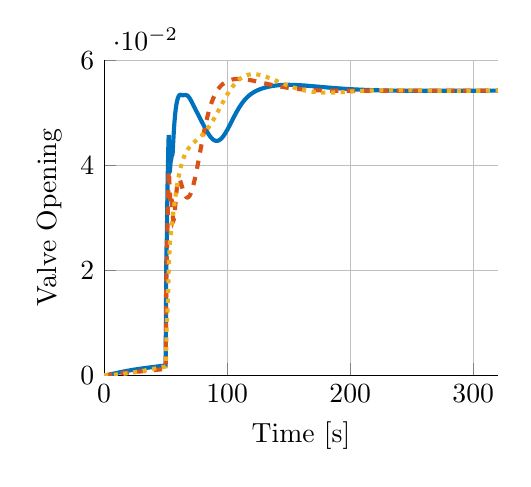
\begin{tikzpicture}

\begin{axis}[%
width=5cm,
height=4cm,
at={(0\linewidth,0\linewidth)},
scale only axis,
xmin=0,
xmax=320,
xlabel={Time [s]},
xmajorgrids,
ymin=0,
ymax=0.06,
ylabel={Valve Opening},
ymajorgrids,
axis background/.style={fill=white},
% title style={font=\bfseries},
% title={Normalized Recycle Valve Opening},
axis x line*=bottom,
axis y line*=left
]
\addplot [color=mycolor1,solid,line width=1.5pt,forget plot]
  table[row sep=crcr]{%
0	0\\
0.25	0\\
0.5	0\\
0.75	0\\
1	0\\
1.25	0\\
1.5	0\\
1.75	1.21538e-06\\
2	6.9504e-06\\
2.25	1.70383e-05\\
2.5	3.02921e-05\\
2.75	4.50965e-05\\
3	5.99591e-05\\
3.25	7.39074e-05\\
3.5	8.62583e-05\\
3.75	9.66784e-05\\
4	0.000105267\\
4.25	0.000112726\\
4.5	0.000120275\\
4.75	0.00012918\\
5	0.000140273\\
5.25	0.000153731\\
5.5	0.00016922\\
5.75	0.000186022\\
6	0.000203147\\
6.25	0.000219559\\
6.5	0.000234417\\
6.75	0.000247281\\
7	0.000258231\\
7.25	0.00026784\\
7.5	0.000277\\
7.75	0.000286676\\
8	0.000297664\\
8.25	0.000310406\\
8.5	0.000324894\\
8.75	0.000340683\\
9	0.000357006\\
9.25	0.000372969\\
9.5	0.000387778\\
9.75	0.000400935\\
10	0.000412358\\
10.25	0.000422393\\
10.5	0.000431714\\
10.75	0.000441145\\
11	0.000451454\\
11.25	0.000463161\\
11.5	0.000476412\\
11.75	0.000490953\\
12	0.000506201\\
12.25	0.000521392\\
12.5	0.000535783\\
12.75	0.000548831\\
13	0.000560334\\
13.25	0.000570472\\
13.5	0.000579758\\
13.75	0.000588899\\
14	0.000598617\\
14.25	0.000609463\\
14.5	0.000621683\\
14.75	0.000635158\\
15	0.000649443\\
15.25	0.000663878\\
15.5	0.000677764\\
15.75	0.000690537\\
16	0.000701909\\
16.25	0.000711944\\
16.5	0.000721031\\
16.75	0.000729787\\
17	0.000738888\\
17.25	0.000748904\\
17.5	0.000760149\\
17.75	0.000772605\\
18	0.00078593\\
18.25	0.000799548\\
18.5	0.000812797\\
18.75	0.000825099\\
19	0.000836108\\
19.25	0.000845799\\
19.5	0.000854471\\
19.75	0.000862668\\
20	0.000871037\\
20.25	0.000880158\\
20.5	0.000890399\\
20.75	0.00090182\\
21	0.000914159\\
21.25	0.000926901\\
21.5	0.000939412\\
21.75	0.000951105\\
22	0.000961585\\
22.25	0.000970761\\
22.5	0.000978863\\
22.75	0.000986381\\
23	0.000993941\\
23.25	0.00100214\\
23.5	0.00101139\\
23.75	0.00102181\\
24	0.0010332\\
24.25	0.00104509\\
24.5	0.00105687\\
24.75	0.00106794\\
25	0.00107785\\
25.25	0.00108646\\
25.5	0.00109395\\
25.75	0.00110077\\
26	0.00110753\\
26.25	0.00111486\\
26.5	0.0011232\\
26.75	0.00113274\\
27	0.00114331\\
27.25	0.00115448\\
27.5	0.00116564\\
27.75	0.00117616\\
28	0.00118557\\
28.25	0.00119368\\
28.5	0.00120061\\
28.75	0.00120679\\
29	0.00121285\\
29.25	0.00121942\\
29.5	0.001227\\
29.75	0.00123581\\
30	0.00124575\\
30.25	0.00125638\\
30.5	0.0012671\\
30.75	0.00127724\\
31	0.00128629\\
31.25	0.001294\\
31.5	0.00130047\\
31.75	0.00130612\\
32	0.00131158\\
32.25	0.00131753\\
32.5	0.00132452\\
32.75	0.00133281\\
33	0.00134232\\
33.25	0.00135263\\
33.5	0.0013631\\
33.75	0.00137304\\
34	0.00138188\\
34.25	0.00138932\\
34.5	0.00139544\\
34.75	0.00140066\\
35	0.00140564\\
35.25	0.0014111\\
35.5	0.00141765\\
35.75	0.0014256\\
36	0.00143488\\
36.25	0.00144508\\
36.5	0.00145552\\
36.75	0.00146544\\
37	0.00147421\\
37.25	0.0014815\\
37.5	0.00148736\\
37.75	0.00149222\\
38	0.00149679\\
38.25	0.00150187\\
38.5	0.00150811\\
38.75	0.00151587\\
39	0.00152512\\
39.25	0.00153541\\
39.5	0.001546\\
39.75	0.00155606\\
40	0.0015649\\
40.25	0.00157212\\
40.5	0.00157776\\
40.75	0.0015823\\
41	0.0015865\\
41.25	0.00159124\\
41.5	0.00159726\\
41.75	0.00160498\\
42	0.00161437\\
42.25	0.00162492\\
42.5	0.00163584\\
42.75	0.00164619\\
43	0.00165519\\
43.25	0.00166238\\
43.5	0.00166782\\
43.75	0.00167201\\
44	0.00167582\\
44.25	0.00168024\\
44.5	0.00168611\\
44.75	0.0016939\\
45	0.00170357\\
45.25	0.00171457\\
45.5	0.00172599\\
45.75	0.00173675\\
46	0.00174597\\
46.25	0.00175315\\
46.5	0.00175831\\
46.75	0.00176207\\
47	0.00176542\\
47.25	0.0017695\\
47.5	0.00177525\\
47.75	0.00178322\\
48	0.00179335\\
48.25	0.00180498\\
48.5	0.00181706\\
48.75	0.00182835\\
49	0.00183783\\
49.25	0.00184493\\
49.5	0.00184971\\
49.75	0.0018529\\
50	0.00185566\\
50.25	0.0106823\\
50.5	0.0208504\\
50.75	0.0243066\\
51	0.0261291\\
51.25	0.0307344\\
51.5	0.0354162\\
51.75	0.0383866\\
52	0.0411891\\
52.25	0.0441063\\
52.5	0.0457436\\
52.75	0.0431454\\
53	0.0400479\\
53.25	0.0387326\\
53.5	0.0388428\\
53.75	0.0397371\\
54	0.0405224\\
54.25	0.0408794\\
54.5	0.0411239\\
54.75	0.0414452\\
55	0.041782\\
55.25	0.0420426\\
55.5	0.0420536\\
55.75	0.0424731\\
56	0.0435875\\
56.25	0.0447724\\
56.5	0.0457822\\
56.75	0.0467364\\
57	0.0476344\\
57.25	0.0484249\\
57.5	0.0491111\\
57.75	0.0497202\\
58	0.0502684\\
58.25	0.0507522\\
58.5	0.0511703\\
58.75	0.0515347\\
59	0.0518568\\
59.25	0.0521409\\
59.5	0.0523902\\
59.75	0.0526083\\
60	0.0527973\\
60.25	0.0529582\\
60.5	0.0530919\\
60.75	0.0531996\\
61	0.0532826\\
61.25	0.0533427\\
61.5	0.0533821\\
61.75	0.0534034\\
62	0.0534097\\
62.25	0.0534046\\
62.5	0.0533915\\
62.75	0.053374\\
63	0.0533556\\
63.25	0.053339\\
63.5	0.0533263\\
63.75	0.053319\\
64	0.0533173\\
64.25	0.0533206\\
64.5	0.0533279\\
64.75	0.0533373\\
65	0.0533471\\
65.25	0.0533558\\
65.5	0.0533622\\
65.75	0.0533657\\
66	0.053366\\
66.25	0.053363\\
66.5	0.0533561\\
66.75	0.0533446\\
67	0.0533276\\
67.25	0.0533041\\
67.5	0.0532733\\
67.75	0.0532346\\
68	0.053188\\
68.25	0.0531336\\
68.5	0.0530714\\
68.75	0.0530019\\
69	0.0529255\\
69.25	0.0528427\\
69.5	0.0527541\\
69.75	0.0526602\\
70	0.0525617\\
70.25	0.052459\\
70.5	0.0523529\\
70.75	0.0522439\\
71	0.0521325\\
71.25	0.0520193\\
71.5	0.0519047\\
71.75	0.051789\\
72	0.0516727\\
72.25	0.0515561\\
72.5	0.0514393\\
72.75	0.0513226\\
73	0.0512062\\
73.25	0.0510901\\
73.5	0.0509743\\
73.75	0.050859\\
74	0.0507441\\
74.25	0.0506297\\
74.5	0.0505156\\
74.75	0.0504018\\
75	0.0502882\\
75.25	0.0501749\\
75.5	0.0500617\\
75.75	0.0499485\\
76	0.0498353\\
76.25	0.0497221\\
76.5	0.0496087\\
76.75	0.0494951\\
77	0.0493814\\
77.25	0.0492674\\
77.5	0.0491532\\
77.75	0.0490387\\
78	0.0489239\\
78.25	0.048809\\
78.5	0.0486938\\
78.75	0.0485785\\
79	0.048463\\
79.25	0.0483475\\
79.5	0.048232\\
79.75	0.0481166\\
80	0.0480013\\
80.25	0.0478863\\
80.5	0.0477715\\
80.75	0.0476572\\
81	0.0475434\\
81.25	0.0474302\\
81.5	0.0473178\\
81.75	0.0472061\\
82	0.0470955\\
82.25	0.0469858\\
82.5	0.0468773\\
82.75	0.0467701\\
83	0.0466643\\
83.25	0.0465601\\
83.5	0.0464574\\
83.75	0.0463564\\
84	0.0462574\\
84.25	0.0461602\\
84.5	0.0460652\\
84.75	0.0459723\\
85	0.0458818\\
85.25	0.0457936\\
85.5	0.0457079\\
85.75	0.0456249\\
86	0.0455446\\
86.25	0.0454671\\
86.5	0.0453925\\
86.75	0.0453209\\
87	0.0452524\\
87.25	0.045187\\
87.5	0.045125\\
87.75	0.0450663\\
88	0.045011\\
88.25	0.0449592\\
88.5	0.044911\\
88.75	0.0448665\\
89	0.0448256\\
89.25	0.0447885\\
89.5	0.0447551\\
89.75	0.0447257\\
90	0.0447001\\
90.25	0.0446784\\
90.5	0.0446607\\
90.75	0.044647\\
91	0.0446372\\
91.25	0.0446315\\
91.5	0.0446299\\
91.75	0.0446322\\
92	0.0446386\\
92.25	0.0446489\\
92.5	0.0446633\\
92.75	0.0446817\\
93	0.044704\\
93.25	0.0447303\\
93.5	0.0447604\\
93.75	0.0447944\\
94	0.0448322\\
94.25	0.0448737\\
94.5	0.044919\\
94.75	0.0449678\\
95	0.0450203\\
95.25	0.0450762\\
95.5	0.0451356\\
95.75	0.0451983\\
96	0.0452643\\
96.25	0.0453334\\
96.5	0.0454056\\
96.75	0.0454809\\
97	0.045559\\
97.25	0.0456399\\
97.5	0.0457235\\
97.75	0.0458098\\
98	0.0458985\\
98.25	0.0459896\\
98.5	0.0460829\\
98.75	0.0461785\\
99	0.0462761\\
99.25	0.0463756\\
99.5	0.046477\\
99.75	0.0465801\\
100	0.0466848\\
100.25	0.0467909\\
100.5	0.0468985\\
100.75	0.0470073\\
101	0.0471173\\
101.25	0.0472283\\
101.5	0.0473403\\
101.75	0.0474531\\
102	0.0475666\\
102.25	0.0476808\\
102.5	0.0477954\\
102.75	0.0479105\\
103	0.0480258\\
103.25	0.0481414\\
103.5	0.0482571\\
103.75	0.0483728\\
104	0.0484885\\
104.25	0.048604\\
104.5	0.0487192\\
104.75	0.0488342\\
105	0.0489487\\
105.25	0.0490628\\
105.5	0.0491762\\
105.75	0.0492891\\
106	0.0494013\\
106.25	0.0495127\\
106.5	0.0496232\\
106.75	0.0497329\\
107	0.0498417\\
107.25	0.0499494\\
107.5	0.0500561\\
107.75	0.0501617\\
108	0.0502662\\
108.25	0.0503694\\
108.5	0.0504715\\
108.75	0.0505723\\
109	0.0506718\\
109.25	0.0507699\\
109.5	0.0508667\\
109.75	0.0509622\\
110	0.0510562\\
110.25	0.0511488\\
110.5	0.05124\\
110.75	0.0513297\\
111	0.051418\\
111.25	0.0515047\\
111.5	0.05159\\
111.75	0.0516738\\
112	0.0517561\\
112.25	0.0518369\\
112.5	0.0519162\\
112.75	0.051994\\
113	0.0520703\\
113.25	0.0521451\\
113.5	0.0522184\\
113.75	0.0522903\\
114	0.0523607\\
114.25	0.0524296\\
114.5	0.0524971\\
114.75	0.0525632\\
115	0.0526279\\
115.25	0.0526912\\
115.5	0.052753\\
115.75	0.0528136\\
116	0.0528728\\
116.25	0.0529306\\
116.5	0.0529872\\
116.75	0.0530425\\
117	0.0530965\\
117.25	0.0531493\\
117.5	0.0532009\\
117.75	0.0532513\\
118	0.0533005\\
118.25	0.0533486\\
118.5	0.0533956\\
118.75	0.0534415\\
119	0.0534863\\
119.25	0.05353\\
119.5	0.0535727\\
119.75	0.0536145\\
120	0.0536552\\
120.25	0.053695\\
120.5	0.0537339\\
120.75	0.0537719\\
121	0.053809\\
121.25	0.0538452\\
121.5	0.0538806\\
121.75	0.0539152\\
122	0.053949\\
122.25	0.053982\\
122.5	0.0540143\\
122.75	0.0540459\\
123	0.0540767\\
123.25	0.0541069\\
123.5	0.0541363\\
123.75	0.0541652\\
124	0.0541934\\
124.25	0.054221\\
124.5	0.054248\\
124.75	0.0542744\\
125	0.0543003\\
125.25	0.0543256\\
125.5	0.0543504\\
125.75	0.0543747\\
126	0.0543985\\
126.25	0.0544218\\
126.5	0.0544446\\
126.75	0.054467\\
127	0.0544889\\
127.25	0.0545103\\
127.5	0.0545314\\
127.75	0.054552\\
128	0.0545723\\
128.25	0.0545921\\
128.5	0.0546116\\
128.75	0.0546306\\
129	0.0546494\\
129.25	0.0546677\\
129.5	0.0546857\\
129.75	0.0547034\\
130	0.0547207\\
130.25	0.0547377\\
130.5	0.0547544\\
130.75	0.0547708\\
131	0.0547868\\
131.25	0.0548026\\
131.5	0.054818\\
131.75	0.0548332\\
132	0.054848\\
132.25	0.0548626\\
132.5	0.0548769\\
132.75	0.0548909\\
133	0.0549046\\
133.25	0.0549181\\
133.5	0.0549313\\
133.75	0.0549442\\
134	0.0549569\\
134.25	0.0549693\\
134.5	0.0549815\\
134.75	0.0549934\\
135	0.055005\\
135.25	0.0550164\\
135.5	0.0550276\\
135.75	0.0550385\\
136	0.0550491\\
136.25	0.0550596\\
136.5	0.0550697\\
136.75	0.0550797\\
137	0.0550894\\
137.25	0.0550989\\
137.5	0.0551081\\
137.75	0.0551171\\
138	0.0551259\\
138.25	0.0551344\\
138.5	0.0551428\\
138.75	0.0551509\\
139	0.0551587\\
139.25	0.0551664\\
139.5	0.0551738\\
139.75	0.055181\\
140	0.055188\\
140.25	0.0551948\\
140.5	0.0552014\\
140.75	0.0552077\\
141	0.0552139\\
141.25	0.0552198\\
141.5	0.0552255\\
141.75	0.055231\\
142	0.0552363\\
142.25	0.0552414\\
142.5	0.0552464\\
142.75	0.0552511\\
143	0.0552556\\
143.25	0.0552599\\
143.5	0.055264\\
143.75	0.055268\\
144	0.0552717\\
144.25	0.0552753\\
144.5	0.0552786\\
144.75	0.0552818\\
145	0.0552848\\
145.25	0.0552877\\
145.5	0.0552903\\
145.75	0.0552928\\
146	0.0552951\\
146.25	0.0552972\\
146.5	0.0552992\\
146.75	0.055301\\
147	0.0553027\\
147.25	0.0553041\\
147.5	0.0553055\\
147.75	0.0553066\\
148	0.0553076\\
148.25	0.0553085\\
148.5	0.0553092\\
148.75	0.0553098\\
149	0.0553102\\
149.25	0.0553105\\
149.5	0.0553106\\
149.75	0.0553106\\
150	0.0553105\\
150.25	0.0553102\\
150.5	0.0553098\\
150.75	0.0553093\\
151	0.0553086\\
151.25	0.0553078\\
151.5	0.055307\\
151.75	0.0553059\\
152	0.0553048\\
152.25	0.0553036\\
152.5	0.0553022\\
152.75	0.0553007\\
153	0.0552992\\
153.25	0.0552975\\
153.5	0.0552957\\
153.75	0.0552938\\
154	0.0552918\\
154.25	0.0552897\\
154.5	0.0552876\\
154.75	0.0552853\\
155	0.0552829\\
155.25	0.0552805\\
155.5	0.055278\\
155.75	0.0552753\\
156	0.0552726\\
156.25	0.0552699\\
156.5	0.055267\\
156.75	0.0552641\\
157	0.055261\\
157.25	0.055258\\
157.5	0.0552548\\
157.75	0.0552516\\
158	0.0552483\\
158.25	0.0552449\\
158.5	0.0552415\\
158.75	0.055238\\
159	0.0552345\\
159.25	0.0552308\\
159.5	0.0552272\\
159.75	0.0552234\\
160	0.0552197\\
160.25	0.0552158\\
160.5	0.0552119\\
160.75	0.055208\\
161	0.055204\\
161.25	0.0552\\
161.5	0.0551959\\
161.75	0.0551918\\
162	0.0551876\\
162.25	0.0551834\\
162.5	0.0551791\\
162.75	0.0551748\\
163	0.0551705\\
163.25	0.0551661\\
163.5	0.0551617\\
163.75	0.0551573\\
164	0.0551528\\
164.25	0.0551483\\
164.5	0.0551437\\
164.75	0.0551391\\
165	0.0551345\\
165.25	0.0551299\\
165.5	0.0551252\\
165.75	0.0551205\\
166	0.0551158\\
166.25	0.0551111\\
166.5	0.0551063\\
166.75	0.0551015\\
167	0.0550967\\
167.25	0.0550918\\
167.5	0.055087\\
167.75	0.0550821\\
168	0.0550772\\
168.25	0.0550723\\
168.5	0.0550674\\
168.75	0.0550624\\
169	0.0550575\\
169.25	0.0550525\\
169.5	0.0550475\\
169.75	0.0550425\\
170	0.0550375\\
170.25	0.0550324\\
170.5	0.0550274\\
170.75	0.0550223\\
171	0.0550173\\
171.25	0.0550122\\
171.5	0.0550071\\
171.75	0.055002\\
172	0.0549969\\
172.25	0.0549918\\
172.5	0.0549867\\
172.75	0.0549816\\
173	0.0549765\\
173.25	0.0549714\\
173.5	0.0549662\\
173.75	0.0549611\\
174	0.054956\\
174.25	0.0549509\\
174.5	0.0549457\\
174.75	0.0549406\\
175	0.0549355\\
175.25	0.0549303\\
175.5	0.0549252\\
175.75	0.0549201\\
176	0.0549149\\
176.25	0.0549098\\
176.5	0.0549047\\
176.75	0.0548996\\
177	0.0548945\\
177.25	0.0548894\\
177.5	0.0548842\\
177.75	0.0548792\\
178	0.0548741\\
178.25	0.054869\\
178.5	0.0548639\\
178.75	0.0548588\\
179	0.0548538\\
179.25	0.0548487\\
179.5	0.0548437\\
179.75	0.0548386\\
180	0.0548336\\
180.25	0.0548286\\
180.5	0.0548236\\
180.75	0.0548186\\
181	0.0548136\\
181.25	0.0548086\\
181.5	0.0548036\\
181.75	0.0547987\\
182	0.0547937\\
182.25	0.0547888\\
182.5	0.0547839\\
182.75	0.054779\\
183	0.0547741\\
183.25	0.0547693\\
183.5	0.0547644\\
183.75	0.0547596\\
184	0.0547547\\
184.25	0.0547499\\
184.5	0.0547451\\
184.75	0.0547403\\
185	0.0547356\\
185.25	0.0547308\\
185.5	0.0547261\\
185.75	0.0547214\\
186	0.0547167\\
186.25	0.054712\\
186.5	0.0547073\\
186.75	0.0547027\\
187	0.0546981\\
187.25	0.0546935\\
187.5	0.0546889\\
187.75	0.0546843\\
188	0.0546798\\
188.25	0.0546752\\
188.5	0.0546707\\
188.75	0.0546662\\
189	0.0546618\\
189.25	0.0546573\\
189.5	0.0546529\\
189.75	0.0546485\\
190	0.0546441\\
190.25	0.0546397\\
190.5	0.0546354\\
190.75	0.054631\\
191	0.0546267\\
191.25	0.0546225\\
191.5	0.0546182\\
191.75	0.0546139\\
192	0.0546097\\
192.25	0.0546055\\
192.5	0.0546014\\
192.75	0.0545972\\
193	0.0545931\\
193.25	0.054589\\
193.5	0.0545849\\
193.75	0.0545808\\
194	0.0545768\\
194.25	0.0545728\\
194.5	0.0545688\\
194.75	0.0545648\\
195	0.0545608\\
195.25	0.0545569\\
195.5	0.054553\\
195.75	0.0545491\\
196	0.0545453\\
196.25	0.0545414\\
196.5	0.0545376\\
196.75	0.0545339\\
197	0.0545301\\
197.25	0.0545263\\
197.5	0.0545226\\
197.75	0.0545189\\
198	0.0545153\\
198.25	0.0545116\\
198.5	0.054508\\
198.75	0.0545044\\
199	0.0545008\\
199.25	0.0544973\\
199.5	0.0544938\\
199.75	0.0544903\\
200	0.0544868\\
200.25	0.0544833\\
200.5	0.0544799\\
200.75	0.0544765\\
201	0.0544731\\
201.25	0.0544698\\
201.5	0.0544664\\
201.75	0.0544631\\
202	0.0544598\\
202.25	0.0544566\\
202.5	0.0544533\\
202.75	0.0544501\\
203	0.0544469\\
203.25	0.0544438\\
203.5	0.0544406\\
203.75	0.0544375\\
204	0.0544344\\
204.25	0.0544313\\
204.5	0.0544283\\
204.75	0.0544252\\
205	0.0544222\\
205.25	0.0544193\\
205.5	0.0544163\\
205.75	0.0544134\\
206	0.0544105\\
206.25	0.0544076\\
206.5	0.0544047\\
206.75	0.0544019\\
207	0.0543991\\
207.25	0.0543963\\
207.5	0.0543935\\
207.75	0.0543908\\
208	0.054388\\
208.25	0.0543853\\
208.5	0.0543827\\
208.75	0.05438\\
209	0.0543774\\
209.25	0.0543748\\
209.5	0.0543722\\
209.75	0.0543696\\
210	0.0543671\\
210.25	0.0543645\\
210.5	0.054362\\
210.75	0.0543596\\
211	0.0543571\\
211.25	0.0543547\\
211.5	0.0543523\\
211.75	0.0543499\\
212	0.0543475\\
212.25	0.0543452\\
212.5	0.0543429\\
212.75	0.0543406\\
213	0.0543383\\
213.25	0.054336\\
213.5	0.0543338\\
213.75	0.0543316\\
214	0.0543294\\
214.25	0.0543272\\
214.5	0.054325\\
214.75	0.0543229\\
215	0.0543208\\
215.25	0.0543187\\
215.5	0.0543166\\
215.75	0.0543146\\
216	0.0543126\\
216.25	0.0543105\\
216.5	0.0543086\\
216.75	0.0543066\\
217	0.0543046\\
217.25	0.0543027\\
217.5	0.0543008\\
217.75	0.0542989\\
218	0.054297\\
218.25	0.0542952\\
218.5	0.0542934\\
218.75	0.0542915\\
219	0.0542897\\
219.25	0.054288\\
219.5	0.0542862\\
219.75	0.0542845\\
220	0.0542828\\
220.25	0.0542811\\
220.5	0.0542794\\
220.75	0.0542777\\
221	0.0542761\\
221.25	0.0542745\\
221.5	0.0542728\\
221.75	0.0542713\\
222	0.0542697\\
222.25	0.0542681\\
222.5	0.0542666\\
222.75	0.0542651\\
223	0.0542636\\
223.25	0.0542621\\
223.5	0.0542606\\
223.75	0.0542592\\
224	0.0542577\\
224.25	0.0542563\\
224.5	0.0542549\\
224.75	0.0542535\\
225	0.0542522\\
225.25	0.0542508\\
225.5	0.0542495\\
225.75	0.0542482\\
226	0.0542469\\
226.25	0.0542456\\
226.5	0.0542443\\
226.75	0.0542431\\
227	0.0542418\\
227.25	0.0542406\\
227.5	0.0542394\\
227.75	0.0542382\\
228	0.054237\\
228.25	0.0542359\\
228.5	0.0542347\\
228.75	0.0542336\\
229	0.0542325\\
229.25	0.0542314\\
229.5	0.0542303\\
229.75	0.0542292\\
230	0.0542282\\
230.25	0.0542271\\
230.5	0.0542261\\
230.75	0.0542251\\
231	0.0542241\\
231.25	0.0542231\\
231.5	0.0542221\\
231.75	0.0542211\\
232	0.0542202\\
232.25	0.0542193\\
232.5	0.0542183\\
232.75	0.0542174\\
233	0.0542165\\
233.25	0.0542156\\
233.5	0.0542148\\
233.75	0.0542139\\
234	0.0542131\\
234.25	0.0542122\\
234.5	0.0542114\\
234.75	0.0542106\\
235	0.0542098\\
235.25	0.054209\\
235.5	0.0542083\\
235.75	0.0542075\\
236	0.0542068\\
236.25	0.054206\\
236.5	0.0542053\\
236.75	0.0542046\\
237	0.0542039\\
237.25	0.0542032\\
237.5	0.0542025\\
237.75	0.0542018\\
238	0.0542012\\
238.25	0.0542005\\
238.5	0.0541999\\
238.75	0.0541993\\
239	0.0541987\\
239.25	0.054198\\
239.5	0.0541975\\
239.75	0.0541969\\
240	0.0541963\\
240.25	0.0541957\\
240.5	0.0541952\\
240.75	0.0541946\\
241	0.0541941\\
241.25	0.0541936\\
241.5	0.0541931\\
241.75	0.0541925\\
242	0.054192\\
242.25	0.0541916\\
242.5	0.0541911\\
242.75	0.0541906\\
243	0.0541901\\
243.25	0.0541897\\
243.5	0.0541893\\
243.75	0.0541888\\
244	0.0541884\\
244.25	0.054188\\
244.5	0.0541876\\
244.75	0.0541872\\
245	0.0541868\\
245.25	0.0541864\\
245.5	0.054186\\
245.75	0.0541856\\
246	0.0541853\\
246.25	0.0541849\\
246.5	0.0541846\\
246.75	0.0541842\\
247	0.0541839\\
247.25	0.0541836\\
247.5	0.0541833\\
247.75	0.054183\\
248	0.0541827\\
248.25	0.0541824\\
248.5	0.0541821\\
248.75	0.0541818\\
249	0.0541815\\
249.25	0.0541813\\
249.5	0.054181\\
249.75	0.0541808\\
250	0.0541805\\
250.25	0.0541803\\
250.5	0.05418\\
250.75	0.0541798\\
251	0.0541796\\
251.25	0.0541794\\
251.5	0.0541792\\
251.75	0.054179\\
252	0.0541788\\
252.25	0.0541786\\
252.5	0.0541784\\
252.75	0.0541782\\
253	0.054178\\
253.25	0.0541779\\
253.5	0.0541777\\
253.75	0.0541776\\
254	0.0541774\\
254.25	0.0541773\\
254.5	0.0541771\\
254.75	0.054177\\
255	0.0541769\\
255.25	0.0541767\\
255.5	0.0541766\\
255.75	0.0541765\\
256	0.0541764\\
256.25	0.0541763\\
256.5	0.0541762\\
256.75	0.0541761\\
257	0.054176\\
257.25	0.0541759\\
257.5	0.0541758\\
257.75	0.0541757\\
258	0.0541757\\
258.25	0.0541756\\
258.5	0.0541755\\
258.75	0.0541755\\
259	0.0541754\\
259.25	0.0541753\\
259.5	0.0541753\\
259.75	0.0541752\\
260	0.0541752\\
260.25	0.0541752\\
260.5	0.0541751\\
260.75	0.0541751\\
261	0.0541751\\
261.25	0.054175\\
261.5	0.054175\\
261.75	0.054175\\
262	0.054175\\
262.25	0.054175\\
262.5	0.054175\\
262.75	0.054175\\
263	0.054175\\
263.25	0.054175\\
263.5	0.054175\\
263.75	0.054175\\
264	0.054175\\
264.25	0.054175\\
264.5	0.054175\\
264.75	0.054175\\
265	0.0541751\\
265.25	0.0541751\\
265.5	0.0541751\\
265.75	0.0541751\\
266	0.0541752\\
266.25	0.0541752\\
266.5	0.0541752\\
266.75	0.0541753\\
267	0.0541753\\
267.25	0.0541754\\
267.5	0.0541754\\
267.75	0.0541755\\
268	0.0541755\\
268.25	0.0541756\\
268.5	0.0541756\\
268.75	0.0541757\\
269	0.0541757\\
269.25	0.0541758\\
269.5	0.0541759\\
269.75	0.0541759\\
270	0.054176\\
270.25	0.0541761\\
270.5	0.0541761\\
270.75	0.0541762\\
271	0.0541763\\
271.25	0.0541764\\
271.5	0.0541765\\
271.75	0.0541765\\
272	0.0541766\\
272.25	0.0541767\\
272.5	0.0541768\\
272.75	0.0541769\\
273	0.054177\\
273.25	0.054177\\
273.5	0.0541771\\
273.75	0.0541772\\
274	0.0541773\\
274.25	0.0541774\\
274.5	0.0541775\\
274.75	0.0541776\\
275	0.0541777\\
275.25	0.0541778\\
275.5	0.0541779\\
275.75	0.054178\\
276	0.0541781\\
276.25	0.0541782\\
276.5	0.0541783\\
276.75	0.0541784\\
277	0.0541785\\
277.25	0.0541786\\
277.5	0.0541787\\
277.75	0.0541789\\
278	0.054179\\
278.25	0.0541791\\
278.5	0.0541792\\
278.75	0.0541793\\
279	0.0541794\\
279.25	0.0541795\\
279.5	0.0541796\\
279.75	0.0541798\\
280	0.0541799\\
280.25	0.05418\\
280.5	0.0541801\\
280.75	0.0541802\\
281	0.0541803\\
281.25	0.0541805\\
281.5	0.0541806\\
281.75	0.0541807\\
282	0.0541808\\
282.25	0.0541809\\
282.5	0.0541811\\
282.75	0.0541812\\
283	0.0541813\\
283.25	0.0541814\\
283.5	0.0541815\\
283.75	0.0541817\\
284	0.0541818\\
284.25	0.0541819\\
284.5	0.054182\\
284.75	0.0541822\\
285	0.0541823\\
285.25	0.0541824\\
285.5	0.0541825\\
285.75	0.0541827\\
286	0.0541828\\
286.25	0.0541829\\
286.5	0.054183\\
286.75	0.0541832\\
287	0.0541833\\
287.25	0.0541834\\
287.5	0.0541835\\
287.75	0.0541837\\
288	0.0541838\\
288.25	0.0541839\\
288.5	0.054184\\
288.75	0.0541842\\
289	0.0541843\\
289.25	0.0541844\\
289.5	0.0541845\\
289.75	0.0541847\\
290	0.0541848\\
290.25	0.0541849\\
290.5	0.054185\\
290.75	0.0541852\\
291	0.0541853\\
291.25	0.0541854\\
291.5	0.0541855\\
291.75	0.0541857\\
292	0.0541858\\
292.25	0.0541859\\
292.5	0.054186\\
292.75	0.0541862\\
293	0.0541863\\
293.25	0.0541864\\
293.5	0.0541865\\
293.75	0.0541866\\
294	0.0541868\\
294.25	0.0541869\\
294.5	0.054187\\
294.75	0.0541871\\
295	0.0541873\\
295.25	0.0541874\\
295.5	0.0541875\\
295.75	0.0541876\\
296	0.0541877\\
296.25	0.0541878\\
296.5	0.054188\\
296.75	0.0541881\\
297	0.0541882\\
297.25	0.0541883\\
297.5	0.0541884\\
297.75	0.0541886\\
298	0.0541887\\
298.25	0.0541888\\
298.5	0.0541889\\
298.75	0.054189\\
299	0.0541891\\
299.25	0.0541892\\
299.5	0.0541894\\
299.75	0.0541895\\
300	0.0541896\\
300.25	0.0541897\\
300.5	0.0541898\\
300.75	0.0541899\\
301	0.05419\\
301.25	0.0541901\\
301.5	0.0541903\\
301.75	0.0541904\\
302	0.0541905\\
302.25	0.0541906\\
302.5	0.0541907\\
302.75	0.0541908\\
303	0.0541909\\
303.25	0.054191\\
303.5	0.0541911\\
303.75	0.0541912\\
304	0.0541913\\
304.25	0.0541914\\
304.5	0.0541915\\
304.75	0.0541916\\
305	0.0541917\\
305.25	0.0541918\\
305.5	0.0541919\\
305.75	0.054192\\
306	0.0541921\\
306.25	0.0541922\\
306.5	0.0541923\\
306.75	0.0541924\\
307	0.0541925\\
307.25	0.0541926\\
307.5	0.0541927\\
307.75	0.0541928\\
308	0.0541929\\
308.25	0.054193\\
308.5	0.0541931\\
308.75	0.0541932\\
309	0.0541933\\
309.25	0.0541934\\
309.5	0.0541935\\
309.75	0.0541936\\
310	0.0541937\\
310.25	0.0541938\\
310.5	0.0541939\\
310.75	0.0541939\\
311	0.054194\\
311.25	0.0541941\\
311.5	0.0541942\\
311.75	0.0541943\\
312	0.0541944\\
312.25	0.0541945\\
312.5	0.0541946\\
312.75	0.0541946\\
313	0.0541947\\
313.25	0.0541948\\
313.5	0.0541949\\
313.75	0.054195\\
314	0.0541951\\
314.25	0.0541951\\
314.5	0.0541952\\
314.75	0.0541953\\
315	0.0541954\\
315.25	0.0541955\\
315.5	0.0541955\\
315.75	0.0541956\\
316	0.0541957\\
316.25	0.0541958\\
316.5	0.0541958\\
316.75	0.0541959\\
317	0.054196\\
317.25	0.0541961\\
317.5	0.0541961\\
317.75	0.0541962\\
318	0.0541963\\
318.25	0.0541964\\
318.5	0.0541964\\
318.75	0.0541965\\
319	0.0541966\\
319.25	0.0541966\\
319.5	0.0541967\\
319.75	0.0541968\\
320	0.0541968\\
320.25	0.0541969\\
320.5	0.054197\\
320.75	0.054197\\
321	0.0541971\\
321.25	0.0541972\\
321.5	0.0541972\\
321.75	0.0541973\\
322	0.0541974\\
322.25	0.0541974\\
322.5	0.0541975\\
322.75	0.0541975\\
323	0.0541976\\
323.25	0.0541977\\
323.5	0.0541977\\
323.75	0.0541978\\
324	0.0541978\\
324.25	0.0541979\\
324.5	0.054198\\
324.75	0.054198\\
325	0.0541981\\
325.25	0.0541981\\
325.5	0.0541982\\
325.75	0.0541982\\
326	0.0541983\\
326.25	0.0541984\\
326.5	0.0541984\\
326.75	0.0541985\\
327	0.0541985\\
327.25	0.0541986\\
327.5	0.0541986\\
327.75	0.0541987\\
328	0.0541987\\
328.25	0.0541988\\
328.5	0.0541988\\
328.75	0.0541989\\
329	0.0541989\\
329.25	0.054199\\
329.5	0.054199\\
329.75	0.0541991\\
330	0.0541991\\
330.25	0.0541991\\
330.5	0.0541992\\
330.75	0.0541992\\
331	0.0541993\\
331.25	0.0541993\\
331.5	0.0541994\\
331.75	0.0541994\\
332	0.0541995\\
332.25	0.0541995\\
332.5	0.0541995\\
332.75	0.0541996\\
333	0.0541996\\
333.25	0.0541997\\
333.5	0.0541997\\
333.75	0.0541997\\
334	0.0541998\\
334.25	0.0541998\\
334.5	0.0541999\\
334.75	0.0541999\\
335	0.0541999\\
335.25	0.0542\\
335.5	0.0542\\
335.75	0.0542\\
336	0.0542001\\
336.25	0.0542001\\
336.5	0.0542001\\
336.75	0.0542002\\
337	0.0542002\\
337.25	0.0542002\\
337.5	0.0542003\\
337.75	0.0542003\\
338	0.0542003\\
338.25	0.0542004\\
338.5	0.0542004\\
338.75	0.0542004\\
339	0.0542005\\
339.25	0.0542005\\
339.5	0.0542005\\
339.75	0.0542006\\
340	0.0542006\\
340.25	0.0542006\\
340.5	0.0542006\\
340.75	0.0542007\\
341	0.0542007\\
341.25	0.0542007\\
341.5	0.0542008\\
341.75	0.0542008\\
342	0.0542008\\
342.25	0.0542008\\
342.5	0.0542009\\
342.75	0.0542009\\
343	0.0542009\\
343.25	0.0542009\\
343.5	0.054201\\
343.75	0.054201\\
344	0.054201\\
344.25	0.054201\\
344.5	0.0542011\\
344.75	0.0542011\\
345	0.0542011\\
345.25	0.0542011\\
345.5	0.0542011\\
345.75	0.0542012\\
346	0.0542012\\
346.25	0.0542012\\
346.5	0.0542012\\
346.75	0.0542012\\
347	0.0542013\\
347.25	0.0542013\\
347.5	0.0542013\\
347.75	0.0542013\\
348	0.0542013\\
348.25	0.0542014\\
348.5	0.0542014\\
348.75	0.0542014\\
349	0.0542014\\
349.25	0.0542014\\
349.5	0.0542014\\
349.75	0.0542015\\
350	0.0542015\\
350.25	0.0542015\\
350.5	0.0542015\\
350.75	0.0542015\\
351	0.0542015\\
351.25	0.0542016\\
351.5	0.0542016\\
351.75	0.0542016\\
352	0.0542016\\
352.25	0.0542016\\
352.5	0.0542016\\
352.75	0.0542016\\
353	0.0542017\\
353.25	0.0542017\\
353.5	0.0542017\\
353.75	0.0542017\\
354	0.0542017\\
354.25	0.0542017\\
354.5	0.0542017\\
354.75	0.0542017\\
355	0.0542018\\
355.25	0.0542018\\
355.5	0.0542018\\
355.75	0.0542018\\
356	0.0542018\\
356.25	0.0542018\\
356.5	0.0542018\\
356.75	0.0542018\\
357	0.0542018\\
357.25	0.0542018\\
357.5	0.0542019\\
357.75	0.0542019\\
358	0.0542019\\
358.25	0.0542019\\
358.5	0.0542019\\
358.75	0.0542019\\
359	0.0542019\\
359.25	0.0542019\\
359.5	0.0542019\\
359.75	0.0542019\\
360	0.0542019\\
360.25	0.0542019\\
360.5	0.054202\\
360.75	0.054202\\
361	0.054202\\
361.25	0.054202\\
361.5	0.054202\\
361.75	0.054202\\
362	0.054202\\
362.25	0.054202\\
362.5	0.054202\\
362.75	0.054202\\
363	0.054202\\
363.25	0.054202\\
363.5	0.054202\\
363.75	0.054202\\
364	0.054202\\
364.25	0.054202\\
364.5	0.054202\\
364.75	0.0542021\\
365	0.0542021\\
365.25	0.0542021\\
365.5	0.0542021\\
365.75	0.0542021\\
366	0.0542021\\
366.25	0.0542021\\
366.5	0.0542021\\
366.75	0.0542021\\
367	0.0542021\\
367.25	0.0542021\\
367.5	0.0542021\\
367.75	0.0542021\\
368	0.0542021\\
368.25	0.0542021\\
368.5	0.0542021\\
368.75	0.0542021\\
369	0.0542021\\
369.25	0.0542021\\
369.5	0.0542021\\
369.75	0.0542021\\
370	0.0542021\\
370.25	0.0542021\\
370.5	0.0542021\\
370.75	0.0542021\\
371	0.0542021\\
371.25	0.0542021\\
371.5	0.0542021\\
371.75	0.0542021\\
372	0.0542021\\
372.25	0.0542021\\
372.5	0.0542021\\
372.75	0.0542021\\
373	0.0542021\\
373.25	0.0542021\\
373.5	0.0542021\\
373.75	0.0542021\\
374	0.0542021\\
374.25	0.0542021\\
374.5	0.0542021\\
374.75	0.0542021\\
375	0.0542021\\
375.25	0.0542021\\
375.5	0.0542021\\
375.75	0.0542021\\
376	0.0542021\\
376.25	0.0542021\\
376.5	0.0542021\\
376.75	0.0542021\\
377	0.0542021\\
377.25	0.0542021\\
377.5	0.0542021\\
377.75	0.0542021\\
378	0.0542021\\
378.25	0.0542021\\
378.5	0.0542021\\
378.75	0.0542021\\
379	0.0542021\\
379.25	0.0542021\\
379.5	0.0542021\\
379.75	0.0542021\\
380	0.0542021\\
380.25	0.0542021\\
380.5	0.0542021\\
380.75	0.0542021\\
381	0.0542021\\
381.25	0.0542021\\
381.5	0.0542021\\
381.75	0.0542021\\
382	0.0542021\\
382.25	0.0542021\\
382.5	0.0542021\\
382.75	0.0542021\\
383	0.0542021\\
383.25	0.0542021\\
383.5	0.0542021\\
383.75	0.0542021\\
384	0.0542021\\
384.25	0.0542021\\
384.5	0.0542021\\
384.75	0.0542021\\
385	0.0542021\\
385.25	0.0542021\\
385.5	0.0542021\\
385.75	0.0542021\\
386	0.0542021\\
386.25	0.0542021\\
386.5	0.0542021\\
386.75	0.0542021\\
387	0.0542021\\
387.25	0.0542021\\
387.5	0.0542021\\
387.75	0.0542021\\
388	0.0542021\\
388.25	0.0542021\\
388.5	0.0542021\\
388.75	0.0542021\\
389	0.0542021\\
389.25	0.054202\\
389.5	0.054202\\
389.75	0.054202\\
390	0.054202\\
390.25	0.054202\\
390.5	0.054202\\
390.75	0.054202\\
391	0.054202\\
391.25	0.054202\\
391.5	0.054202\\
391.75	0.054202\\
392	0.054202\\
392.25	0.054202\\
392.5	0.054202\\
392.75	0.054202\\
393	0.054202\\
393.25	0.054202\\
393.5	0.054202\\
393.75	0.054202\\
394	0.054202\\
394.25	0.054202\\
394.5	0.054202\\
394.75	0.054202\\
395	0.054202\\
395.25	0.054202\\
395.5	0.054202\\
395.75	0.054202\\
396	0.054202\\
396.25	0.054202\\
396.5	0.054202\\
396.75	0.054202\\
397	0.054202\\
397.25	0.054202\\
397.5	0.054202\\
397.75	0.0542019\\
398	0.0542019\\
398.25	0.0542019\\
398.5	0.0542019\\
398.75	0.0542019\\
399	0.0542019\\
399.25	0.0542019\\
399.5	0.0542019\\
399.75	0.0542019\\
400	0.0542019\\
400.25	0.0542019\\
400.5	0.0542019\\
400.75	0.0542019\\
401	0.0542019\\
401.25	0.0542019\\
401.5	0.0542019\\
401.75	0.0542019\\
402	0.0542019\\
402.25	0.0542019\\
402.5	0.0542019\\
402.75	0.0542019\\
403	0.0542019\\
403.25	0.0542019\\
403.5	0.0542019\\
403.75	0.0542019\\
404	0.0542019\\
404.25	0.0542019\\
404.5	0.0542019\\
404.75	0.0542019\\
405	0.0542019\\
405.25	0.0542019\\
405.5	0.0542019\\
405.75	0.0542019\\
406	0.0542018\\
406.25	0.0542018\\
406.5	0.0542018\\
406.75	0.0542018\\
407	0.0542018\\
407.25	0.0542018\\
407.5	0.0542018\\
407.75	0.0542018\\
408	0.0542018\\
408.25	0.0542018\\
408.5	0.0542018\\
408.75	0.0542018\\
409	0.0542018\\
409.25	0.0542018\\
409.5	0.0542018\\
409.75	0.0542018\\
410	0.0542018\\
410.25	0.0542018\\
410.5	0.0542018\\
410.75	0.0542018\\
411	0.0542018\\
411.25	0.0542018\\
411.5	0.0542018\\
411.75	0.0542018\\
412	0.0542018\\
412.25	0.0542018\\
412.5	0.0542018\\
412.75	0.0542018\\
413	0.0542018\\
413.25	0.0542018\\
413.5	0.0542018\\
413.75	0.0542018\\
414	0.0542018\\
414.25	0.0542018\\
414.5	0.0542018\\
414.75	0.0542018\\
415	0.0542017\\
415.25	0.0542017\\
415.5	0.0542017\\
415.75	0.0542017\\
416	0.0542017\\
416.25	0.0542017\\
416.5	0.0542017\\
416.75	0.0542017\\
417	0.0542017\\
417.25	0.0542017\\
417.5	0.0542017\\
417.75	0.0542017\\
418	0.0542017\\
418.25	0.0542017\\
418.5	0.0542017\\
418.75	0.0542017\\
419	0.0542017\\
419.25	0.0542017\\
419.5	0.0542017\\
419.75	0.0542017\\
420	0.0542017\\
420.25	0.0542017\\
420.5	0.0542017\\
420.75	0.0542017\\
421	0.0542017\\
421.25	0.0542017\\
421.5	0.0542017\\
421.75	0.0542017\\
422	0.0542017\\
422.25	0.0542017\\
422.5	0.0542017\\
422.75	0.0542017\\
423	0.0542017\\
423.25	0.0542017\\
423.5	0.0542017\\
423.75	0.0542017\\
424	0.0542017\\
424.25	0.0542017\\
424.5	0.0542017\\
424.75	0.0542017\\
425	0.0542017\\
425.25	0.0542017\\
425.5	0.0542017\\
425.75	0.0542016\\
426	0.0542016\\
426.25	0.0542016\\
426.5	0.0542016\\
426.75	0.0542016\\
427	0.0542016\\
427.25	0.0542016\\
427.5	0.0542016\\
427.75	0.0542016\\
428	0.0542016\\
428.25	0.0542016\\
428.5	0.0542016\\
428.75	0.0542016\\
429	0.0542016\\
429.25	0.0542016\\
429.5	0.0542016\\
429.75	0.0542016\\
430	0.0542016\\
430.25	0.0542016\\
430.5	0.0542016\\
430.75	0.0542016\\
431	0.0542016\\
431.25	0.0542016\\
431.5	0.0542016\\
431.75	0.0542016\\
432	0.0542016\\
432.25	0.0542016\\
432.5	0.0542016\\
432.75	0.0542016\\
433	0.0542016\\
433.25	0.0542016\\
433.5	0.0542016\\
433.75	0.0542016\\
434	0.0542016\\
434.25	0.0542016\\
434.5	0.0542016\\
434.75	0.0542016\\
435	0.0542016\\
435.25	0.0542016\\
435.5	0.0542016\\
435.75	0.0542016\\
436	0.0542016\\
436.25	0.0542016\\
436.5	0.0542016\\
436.75	0.0542016\\
437	0.0542016\\
437.25	0.0542016\\
437.5	0.0542016\\
437.75	0.0542016\\
438	0.0542016\\
438.25	0.0542016\\
438.5	0.0542016\\
438.75	0.0542016\\
439	0.0542016\\
439.25	0.0542016\\
439.5	0.0542016\\
439.75	0.0542016\\
440	0.0542016\\
440.25	0.0542016\\
440.5	0.0542016\\
440.75	0.0542016\\
441	0.0542016\\
441.25	0.0542015\\
441.5	0.0542015\\
441.75	0.0542015\\
442	0.0542015\\
442.25	0.0542015\\
442.5	0.0542015\\
442.75	0.0542015\\
443	0.0542015\\
443.25	0.0542015\\
443.5	0.0542015\\
443.75	0.0542015\\
444	0.0542015\\
444.25	0.0542015\\
444.5	0.0542015\\
444.75	0.0542015\\
445	0.0542015\\
445.25	0.0542015\\
445.5	0.0542015\\
445.75	0.0542015\\
446	0.0542015\\
446.25	0.0542015\\
446.5	0.0542015\\
446.75	0.0542015\\
447	0.0542015\\
447.25	0.0542015\\
447.5	0.0542015\\
447.75	0.0542015\\
448	0.0542015\\
448.25	0.0542015\\
448.5	0.0542015\\
448.75	0.0542015\\
449	0.0542015\\
449.25	0.0542015\\
449.5	0.0542015\\
449.75	0.0542015\\
450	0.0542015\\
450.25	0.0542015\\
450.5	0.0542015\\
450.75	0.0542015\\
451	0.0542015\\
451.25	0.0542015\\
451.5	0.0542015\\
451.75	0.0542015\\
452	0.0542015\\
452.25	0.0542015\\
452.5	0.0542015\\
452.75	0.0542015\\
453	0.0542015\\
453.25	0.0542015\\
453.5	0.0542015\\
453.75	0.0542015\\
454	0.0542015\\
454.25	0.0542015\\
454.5	0.0542015\\
454.75	0.0542015\\
455	0.0542015\\
455.25	0.0542015\\
455.5	0.0542015\\
455.75	0.0542015\\
456	0.0542015\\
456.25	0.0542015\\
456.5	0.0542015\\
456.75	0.0542015\\
457	0.0542015\\
457.25	0.0542015\\
457.5	0.0542015\\
457.75	0.0542015\\
458	0.0542015\\
458.25	0.0542015\\
458.5	0.0542015\\
458.75	0.0542015\\
459	0.0542015\\
459.25	0.0542015\\
459.5	0.0542015\\
459.75	0.0542015\\
460	0.0542015\\
460.25	0.0542015\\
460.5	0.0542015\\
460.75	0.0542015\\
461	0.0542015\\
461.25	0.0542015\\
461.5	0.0542015\\
461.75	0.0542015\\
462	0.0542015\\
462.25	0.0542015\\
462.5	0.0542015\\
462.75	0.0542015\\
463	0.0542015\\
463.25	0.0542015\\
463.5	0.0542015\\
463.75	0.0542015\\
464	0.0542015\\
464.25	0.0542015\\
464.5	0.0542015\\
464.75	0.0542015\\
465	0.0542015\\
465.25	0.0542015\\
465.5	0.0542015\\
465.75	0.0542015\\
466	0.0542015\\
466.25	0.0542015\\
466.5	0.0542015\\
466.75	0.0542015\\
467	0.0542015\\
467.25	0.0542015\\
467.5	0.0542015\\
467.75	0.0542015\\
468	0.0542015\\
468.25	0.0542015\\
468.5	0.0542015\\
468.75	0.0542015\\
469	0.0542015\\
469.25	0.0542015\\
469.5	0.0542015\\
469.75	0.0542015\\
470	0.0542015\\
470.25	0.0542015\\
470.5	0.0542015\\
470.75	0.0542015\\
471	0.0542015\\
471.25	0.0542015\\
471.5	0.0542015\\
471.75	0.0542015\\
472	0.0542015\\
472.25	0.0542015\\
472.5	0.0542015\\
472.75	0.0542015\\
473	0.0542015\\
473.25	0.0542015\\
473.5	0.0542015\\
473.75	0.0542015\\
474	0.0542015\\
474.25	0.0542015\\
474.5	0.0542015\\
474.75	0.0542015\\
475	0.0542015\\
475.25	0.0542015\\
475.5	0.0542015\\
475.75	0.0542015\\
476	0.0542015\\
476.25	0.0542015\\
476.5	0.0542015\\
476.75	0.0542015\\
477	0.0542015\\
477.25	0.0542015\\
477.5	0.0542015\\
477.75	0.0542015\\
478	0.0542015\\
478.25	0.0542015\\
478.5	0.0542015\\
478.75	0.0542015\\
479	0.0542015\\
479.25	0.0542015\\
479.5	0.0542015\\
479.75	0.0542015\\
480	0.0542015\\
480.25	0.0542015\\
480.5	0.0542015\\
480.75	0.0542015\\
481	0.0542015\\
481.25	0.0542015\\
481.5	0.0542015\\
481.75	0.0542015\\
482	0.0542015\\
482.25	0.0542015\\
482.5	0.0542015\\
482.75	0.0542015\\
483	0.0542015\\
483.25	0.0542015\\
483.5	0.0542015\\
483.75	0.0542015\\
484	0.0542015\\
484.25	0.0542015\\
484.5	0.0542015\\
484.75	0.0542015\\
485	0.0542015\\
485.25	0.0542015\\
485.5	0.0542015\\
485.75	0.0542015\\
486	0.0542015\\
486.25	0.0542015\\
486.5	0.0542015\\
486.75	0.0542015\\
487	0.0542015\\
487.25	0.0542015\\
487.5	0.0542015\\
487.75	0.0542015\\
488	0.0542015\\
488.25	0.0542015\\
488.5	0.0542015\\
488.75	0.0542015\\
489	0.0542015\\
489.25	0.0542015\\
489.5	0.0542015\\
489.75	0.0542015\\
490	0.0542015\\
490.25	0.0542015\\
490.5	0.0542015\\
490.75	0.0542015\\
491	0.0542015\\
491.25	0.0542015\\
491.5	0.0542015\\
491.75	0.0542015\\
492	0.0542015\\
492.25	0.0542015\\
492.5	0.0542015\\
492.75	0.0542015\\
493	0.0542015\\
493.25	0.0542015\\
493.5	0.0542015\\
493.75	0.0542015\\
494	0.0542015\\
494.25	0.0542015\\
494.5	0.0542015\\
494.75	0.0542015\\
495	0.0542015\\
495.25	0.0542015\\
495.5	0.0542015\\
495.75	0.0542015\\
496	0.0542015\\
496.25	0.0542015\\
496.5	0.0542015\\
496.75	0.0542015\\
497	0.0542015\\
497.25	0.0542015\\
497.5	0.0542015\\
497.75	0.0542015\\
498	0.0542015\\
498.25	0.0542015\\
498.5	0.0542015\\
498.75	0.0542015\\
499	0.0542015\\
499.25	0.0542015\\
499.5	0.0542015\\
499.75	0.0542015\\
};
\addplot [color=mycolor2,dashed,line width=1.5pt,forget plot]
  table[row sep=crcr]{%
0	0\\
0.25	0\\
0.5	0\\
0.75	0\\
1	0\\
1.25	0\\
1.5	0\\
1.75	0\\
2	8.48789e-07\\
2.25	3.74418e-06\\
2.5	8.50018e-06\\
2.75	1.47428e-05\\
3	2.2059e-05\\
3.25	3.00366e-05\\
3.5	3.82816e-05\\
3.75	4.64519e-05\\
4	5.42697e-05\\
4.25	6.15603e-05\\
4.5	6.83509e-05\\
4.75	7.48495e-05\\
5	8.13278e-05\\
5.25	8.80406e-05\\
5.5	9.51821e-05\\
5.75	0.000102858\\
6	0.000111073\\
6.25	0.000119742\\
6.5	0.000128702\\
6.75	0.000137756\\
7	0.000146708\\
7.25	0.00015541\\
7.5	0.000163782\\
7.75	0.000171816\\
8	0.000179572\\
8.25	0.000187152\\
8.5	0.000194674\\
8.75	0.000202251\\
9	0.00020996\\
9.25	0.000217837\\
9.5	0.000225866\\
9.75	0.000233993\\
10	0.00024214\\
10.25	0.00025022\\
10.5	0.000258158\\
10.75	0.000265906\\
11	0.000273446\\
11.25	0.000280793\\
11.5	0.000287987\\
11.75	0.000295082\\
12	0.000302136\\
12.25	0.000309195\\
12.5	0.000316286\\
12.75	0.000323416\\
13	0.00033057\\
13.25	0.000337717\\
13.5	0.00034482\\
13.75	0.000351843\\
14	0.000358756\\
14.25	0.000365547\\
14.5	0.000372215\\
14.75	0.000378775\\
15	0.000385252\\
15.25	0.000391671\\
15.5	0.00039806\\
15.75	0.000404435\\
16	0.000410807\\
16.25	0.000417172\\
16.5	0.00042352\\
16.75	0.000429836\\
17	0.000436102\\
17.25	0.000442303\\
17.5	0.000448431\\
17.75	0.000454483\\
18	0.000460464\\
18.25	0.000466384\\
18.5	0.000472257\\
18.75	0.000478097\\
19	0.000483915\\
19.25	0.000489717\\
19.5	0.000495507\\
19.75	0.000501282\\
20	0.000507035\\
20.25	0.00051276\\
20.5	0.00051845\\
20.75	0.000524099\\
21	0.000529707\\
21.25	0.000535274\\
21.5	0.000540807\\
21.75	0.000546311\\
22	0.000551794\\
22.25	0.000557263\\
22.5	0.000562724\\
22.75	0.00056818\\
23	0.00057363\\
23.25	0.000579074\\
23.5	0.000584509\\
23.75	0.000589931\\
24	0.00059534\\
24.25	0.000600733\\
24.5	0.000606111\\
24.75	0.000611478\\
25	0.000616837\\
25.25	0.000622191\\
25.5	0.000627545\\
25.75	0.000632903\\
26	0.000638266\\
26.25	0.000643637\\
26.5	0.000649014\\
26.75	0.000654397\\
27	0.000659785\\
27.25	0.000665177\\
27.5	0.000670571\\
27.75	0.000675969\\
28	0.000681372\\
28.25	0.00068678\\
28.5	0.000692197\\
28.75	0.000697624\\
29	0.000703063\\
29.25	0.000708515\\
29.5	0.000713982\\
29.75	0.000719463\\
30	0.000724957\\
30.25	0.000730465\\
30.5	0.000735984\\
30.75	0.000741516\\
31	0.000747059\\
31.25	0.000752613\\
31.5	0.000758179\\
31.75	0.000763757\\
32	0.000769349\\
32.25	0.000774955\\
32.5	0.000780576\\
32.75	0.00078621\\
33	0.00079186\\
33.25	0.000797523\\
33.5	0.000803199\\
33.75	0.000808888\\
34	0.000814588\\
34.25	0.000820299\\
34.5	0.000826021\\
34.75	0.000831753\\
35	0.000837495\\
35.25	0.000843247\\
35.5	0.00084901\\
35.75	0.000854782\\
36	0.000860565\\
36.25	0.000866356\\
36.5	0.000872157\\
36.75	0.000877966\\
37	0.000883782\\
37.25	0.000889604\\
37.5	0.000895433\\
37.75	0.000901267\\
38	0.000907105\\
38.25	0.000912948\\
38.5	0.000918796\\
38.75	0.000924647\\
39	0.000930502\\
39.25	0.00093636\\
39.5	0.00094222\\
39.75	0.000948083\\
40	0.000953948\\
40.25	0.000959814\\
40.5	0.000965681\\
40.75	0.000971548\\
41	0.000977414\\
41.25	0.000983279\\
41.5	0.000989143\\
41.75	0.000995006\\
42	0.00100087\\
42.25	0.00100673\\
42.5	0.00101258\\
42.75	0.00101844\\
43	0.00102429\\
43.25	0.00103014\\
43.5	0.00103598\\
43.75	0.00104182\\
44	0.00104766\\
44.25	0.00105349\\
44.5	0.00105932\\
44.75	0.00106515\\
45	0.00107097\\
45.25	0.00107678\\
45.5	0.00108259\\
45.75	0.0010884\\
46	0.0010942\\
46.25	0.00109999\\
46.5	0.00110578\\
46.75	0.00111156\\
47	0.00111734\\
47.25	0.00112312\\
47.5	0.00112888\\
47.75	0.00113465\\
48	0.0011404\\
48.25	0.00114616\\
48.5	0.0011519\\
48.75	0.00115764\\
49	0.00116338\\
49.25	0.00116911\\
49.5	0.00117484\\
49.75	0.00118056\\
50	0.00118628\\
50.25	0.0063658\\
50.5	0.0172444\\
50.75	0.0208826\\
51	0.0216428\\
51.25	0.0249515\\
51.5	0.0285646\\
51.75	0.0313042\\
52	0.0340314\\
52.25	0.036738\\
52.5	0.0389529\\
52.75	0.0387641\\
53	0.0369547\\
53.25	0.0357285\\
53.5	0.034636\\
53.75	0.0334517\\
54	0.0329026\\
54.25	0.0335724\\
54.5	0.0338922\\
54.75	0.0336261\\
55	0.0332387\\
55.25	0.0327268\\
55.5	0.0318493\\
55.75	0.0308817\\
56	0.0299164\\
56.25	0.029381\\
56.5	0.0295112\\
56.75	0.0299094\\
57	0.0303458\\
57.25	0.0308459\\
57.5	0.0314406\\
57.75	0.0320795\\
58	0.0327253\\
58.25	0.0333866\\
58.5	0.0340626\\
58.75	0.0347197\\
59	0.0353201\\
59.25	0.0358453\\
59.5	0.0362889\\
59.75	0.0366483\\
60	0.0369248\\
60.25	0.0371241\\
60.5	0.0372528\\
60.75	0.0373178\\
61	0.0373258\\
61.25	0.0372843\\
61.5	0.037201\\
61.75	0.0370828\\
62	0.0369365\\
62.25	0.0367679\\
62.5	0.0365826\\
62.75	0.0363855\\
63	0.036181\\
63.25	0.035973\\
63.5	0.035765\\
63.75	0.03556\\
64	0.0353606\\
64.25	0.035169\\
64.5	0.0349869\\
64.75	0.0348159\\
65	0.034657\\
65.25	0.0345112\\
65.5	0.0343791\\
65.75	0.0342611\\
66	0.0341575\\
66.25	0.0340685\\
66.5	0.0339941\\
66.75	0.0339344\\
67	0.0338892\\
67.25	0.0338584\\
67.5	0.0338419\\
67.75	0.0338395\\
68	0.0338511\\
68.25	0.0338764\\
68.5	0.0339152\\
68.75	0.0339673\\
69	0.0340326\\
69.25	0.0341107\\
69.5	0.0342014\\
69.75	0.0343046\\
70	0.0344199\\
70.25	0.034547\\
70.5	0.0346858\\
70.75	0.0348358\\
71	0.0349969\\
71.25	0.0351686\\
71.5	0.0353507\\
71.75	0.0355429\\
72	0.0357447\\
72.25	0.0359558\\
72.5	0.0361759\\
72.75	0.0364045\\
73	0.0366413\\
73.25	0.0368859\\
73.5	0.0371378\\
73.75	0.0373968\\
74	0.0376623\\
74.25	0.037934\\
74.5	0.0382114\\
74.75	0.0384941\\
75	0.0387817\\
75.25	0.0390739\\
75.5	0.03937\\
75.75	0.0396698\\
76	0.0399729\\
76.25	0.0402787\\
76.5	0.0405869\\
76.75	0.0408972\\
77	0.041209\\
77.25	0.041522\\
77.5	0.0418358\\
77.75	0.0421501\\
78	0.0424644\\
78.25	0.0427784\\
78.5	0.0430917\\
78.75	0.0434041\\
79	0.0437151\\
79.25	0.0440244\\
79.5	0.0443318\\
79.75	0.0446369\\
80	0.0449395\\
80.25	0.0452393\\
80.5	0.0455361\\
80.75	0.0458295\\
81	0.0461194\\
81.25	0.0464056\\
81.5	0.0466879\\
81.75	0.0469661\\
82	0.0472399\\
82.25	0.0475094\\
82.5	0.0477743\\
82.75	0.0480345\\
83	0.04829\\
83.25	0.0485405\\
83.5	0.0487861\\
83.75	0.0490266\\
84	0.0492621\\
84.25	0.0494924\\
84.5	0.0497175\\
84.75	0.0499374\\
85	0.0501522\\
85.25	0.0503617\\
85.5	0.050566\\
85.75	0.0507652\\
86	0.0509592\\
86.25	0.051148\\
86.5	0.0513318\\
86.75	0.0515106\\
87	0.0516844\\
87.25	0.0518533\\
87.5	0.0520174\\
87.75	0.0521767\\
88	0.0523313\\
88.25	0.0524813\\
88.5	0.0526267\\
88.75	0.0527678\\
89	0.0529044\\
89.25	0.0530369\\
89.5	0.0531651\\
89.75	0.0532893\\
90	0.0534095\\
90.25	0.0535259\\
90.5	0.0536385\\
90.75	0.0537474\\
91	0.0538527\\
91.25	0.0539546\\
91.5	0.0540531\\
91.75	0.0541483\\
92	0.0542403\\
92.25	0.0543292\\
92.5	0.0544152\\
92.75	0.0544982\\
93	0.0545784\\
93.25	0.0546558\\
93.5	0.0547307\\
93.75	0.0548029\\
94	0.0548727\\
94.25	0.0549401\\
94.5	0.0550052\\
94.75	0.055068\\
95	0.0551286\\
95.25	0.0551872\\
95.5	0.0552437\\
95.75	0.0552983\\
96	0.0553509\\
96.25	0.0554017\\
96.5	0.0554507\\
96.75	0.055498\\
97	0.0555436\\
97.25	0.0555876\\
97.5	0.0556301\\
97.75	0.055671\\
98	0.0557104\\
98.25	0.0557485\\
98.5	0.0557851\\
98.75	0.0558204\\
99	0.0558544\\
99.25	0.0558871\\
99.5	0.0559186\\
99.75	0.0559489\\
100	0.055978\\
100.25	0.056006\\
100.5	0.0560329\\
100.75	0.0560587\\
101	0.0560835\\
101.25	0.0561072\\
101.5	0.05613\\
101.75	0.0561518\\
102	0.0561726\\
102.25	0.0561925\\
102.5	0.0562115\\
102.75	0.0562297\\
103	0.056247\\
103.25	0.0562634\\
103.5	0.056279\\
103.75	0.0562938\\
104	0.0563079\\
104.25	0.0563211\\
104.5	0.0563336\\
104.75	0.0563454\\
105	0.0563564\\
105.25	0.0563668\\
105.5	0.0563764\\
105.75	0.0563854\\
106	0.0563937\\
106.25	0.0564013\\
106.5	0.0564084\\
106.75	0.0564148\\
107	0.0564205\\
107.25	0.0564257\\
107.5	0.0564304\\
107.75	0.0564344\\
108	0.0564379\\
108.25	0.0564408\\
108.5	0.0564432\\
108.75	0.0564451\\
109	0.0564464\\
109.25	0.0564473\\
109.5	0.0564477\\
109.75	0.0564476\\
110	0.056447\\
110.25	0.056446\\
110.5	0.0564445\\
110.75	0.0564426\\
111	0.0564403\\
111.25	0.0564375\\
111.5	0.0564344\\
111.75	0.0564308\\
112	0.0564269\\
112.25	0.0564226\\
112.5	0.0564179\\
112.75	0.0564129\\
113	0.0564076\\
113.25	0.0564019\\
113.5	0.0563958\\
113.75	0.0563895\\
114	0.0563828\\
114.25	0.0563759\\
114.5	0.0563686\\
114.75	0.0563611\\
115	0.0563533\\
115.25	0.0563452\\
115.5	0.0563369\\
115.75	0.0563283\\
116	0.0563195\\
116.25	0.0563104\\
116.5	0.0563011\\
116.75	0.0562916\\
117	0.0562819\\
117.25	0.056272\\
117.5	0.0562618\\
117.75	0.0562515\\
118	0.056241\\
118.25	0.0562304\\
118.5	0.0562195\\
118.75	0.0562085\\
119	0.0561973\\
119.25	0.056186\\
119.5	0.0561745\\
119.75	0.0561629\\
120	0.0561512\\
120.25	0.0561393\\
120.5	0.0561273\\
120.75	0.0561152\\
121	0.056103\\
121.25	0.0560907\\
121.5	0.0560782\\
121.75	0.0560657\\
122	0.0560531\\
122.25	0.0560404\\
122.5	0.0560276\\
122.75	0.0560147\\
123	0.0560018\\
123.25	0.0559888\\
123.5	0.0559757\\
123.75	0.0559626\\
124	0.0559494\\
124.25	0.0559361\\
124.5	0.0559228\\
124.75	0.0559095\\
125	0.0558961\\
125.25	0.0558827\\
125.5	0.0558693\\
125.75	0.0558558\\
126	0.0558423\\
126.25	0.0558288\\
126.5	0.0558152\\
126.75	0.0558017\\
127	0.0557881\\
127.25	0.0557745\\
127.5	0.0557609\\
127.75	0.0557473\\
128	0.0557337\\
128.25	0.0557201\\
128.5	0.0557066\\
128.75	0.055693\\
129	0.0556794\\
129.25	0.0556658\\
129.5	0.0556523\\
129.75	0.0556387\\
130	0.0556252\\
130.25	0.0556117\\
130.5	0.0555983\\
130.75	0.0555848\\
131	0.0555714\\
131.25	0.055558\\
131.5	0.0555447\\
131.75	0.0555313\\
132	0.055518\\
132.25	0.0555048\\
132.5	0.0554916\\
132.75	0.0554784\\
133	0.0554653\\
133.25	0.0554522\\
133.5	0.0554392\\
133.75	0.0554262\\
134	0.0554132\\
134.25	0.0554003\\
134.5	0.0553875\\
134.75	0.0553747\\
135	0.055362\\
135.25	0.0553493\\
135.5	0.0553367\\
135.75	0.0553241\\
136	0.0553116\\
136.25	0.0552991\\
136.5	0.0552868\\
136.75	0.0552744\\
137	0.0552622\\
137.25	0.05525\\
137.5	0.0552379\\
137.75	0.0552258\\
138	0.0552138\\
138.25	0.0552019\\
138.5	0.05519\\
138.75	0.0551782\\
139	0.0551665\\
139.25	0.0551549\\
139.5	0.0551433\\
139.75	0.0551318\\
140	0.0551204\\
140.25	0.055109\\
140.5	0.0550977\\
140.75	0.0550865\\
141	0.0550754\\
141.25	0.0550643\\
141.5	0.0550534\\
141.75	0.0550425\\
142	0.0550316\\
142.25	0.0550209\\
142.5	0.0550102\\
142.75	0.0549996\\
143	0.0549891\\
143.25	0.0549787\\
143.5	0.0549683\\
143.75	0.0549581\\
144	0.0549479\\
144.25	0.0549378\\
144.5	0.0549277\\
144.75	0.0549178\\
145	0.0549079\\
145.25	0.0548981\\
145.5	0.0548884\\
145.75	0.0548788\\
146	0.0548692\\
146.25	0.0548598\\
146.5	0.0548504\\
146.75	0.0548411\\
147	0.0548319\\
147.25	0.0548227\\
147.5	0.0548137\\
147.75	0.0548047\\
148	0.0547958\\
148.25	0.054787\\
148.5	0.0547782\\
148.75	0.0547696\\
149	0.054761\\
149.25	0.0547525\\
149.5	0.0547441\\
149.75	0.0547358\\
150	0.0547275\\
150.25	0.0547193\\
150.5	0.0547112\\
150.75	0.0547032\\
151	0.0546953\\
151.25	0.0546874\\
151.5	0.0546797\\
151.75	0.054672\\
152	0.0546644\\
152.25	0.0546568\\
152.5	0.0546494\\
152.75	0.054642\\
153	0.0546347\\
153.25	0.0546274\\
153.5	0.0546203\\
153.75	0.0546132\\
154	0.0546062\\
154.25	0.0545993\\
154.5	0.0545924\\
154.75	0.0545857\\
155	0.054579\\
155.25	0.0545724\\
155.5	0.0545658\\
155.75	0.0545593\\
156	0.0545529\\
156.25	0.0545466\\
156.5	0.0545404\\
156.75	0.0545342\\
157	0.0545281\\
157.25	0.054522\\
157.5	0.0545161\\
157.75	0.0545102\\
158	0.0545044\\
158.25	0.0544986\\
158.5	0.0544929\\
158.75	0.0544873\\
159	0.0544818\\
159.25	0.0544763\\
159.5	0.0544709\\
159.75	0.0544655\\
160	0.0544603\\
160.25	0.054455\\
160.5	0.0544499\\
160.75	0.0544448\\
161	0.0544398\\
161.25	0.0544349\\
161.5	0.05443\\
161.75	0.0544252\\
162	0.0544204\\
162.25	0.0544157\\
162.5	0.0544111\\
162.75	0.0544065\\
163	0.054402\\
163.25	0.0543976\\
163.5	0.0543932\\
163.75	0.0543889\\
164	0.0543846\\
164.25	0.0543804\\
164.5	0.0543762\\
164.75	0.0543721\\
165	0.0543681\\
165.25	0.0543641\\
165.5	0.0543602\\
165.75	0.0543564\\
166	0.0543525\\
166.25	0.0543488\\
166.5	0.0543451\\
166.75	0.0543415\\
167	0.0543379\\
167.25	0.0543343\\
167.5	0.0543308\\
167.75	0.0543274\\
168	0.054324\\
168.25	0.0543207\\
168.5	0.0543174\\
168.75	0.0543142\\
169	0.054311\\
169.25	0.0543079\\
169.5	0.0543048\\
169.75	0.0543018\\
170	0.0542988\\
170.25	0.0542959\\
170.5	0.054293\\
170.75	0.0542902\\
171	0.0542874\\
171.25	0.0542846\\
171.5	0.0542819\\
171.75	0.0542793\\
172	0.0542766\\
172.25	0.0542741\\
172.5	0.0542715\\
172.75	0.0542691\\
173	0.0542666\\
173.25	0.0542642\\
173.5	0.0542619\\
173.75	0.0542595\\
174	0.0542573\\
174.25	0.054255\\
174.5	0.0542528\\
174.75	0.0542507\\
175	0.0542485\\
175.25	0.0542465\\
175.5	0.0542444\\
175.75	0.0542424\\
176	0.0542404\\
176.25	0.0542385\\
176.5	0.0542366\\
176.75	0.0542348\\
177	0.0542329\\
177.25	0.0542311\\
177.5	0.0542294\\
177.75	0.0542277\\
178	0.054226\\
178.25	0.0542243\\
178.5	0.0542227\\
178.75	0.0542211\\
179	0.0542195\\
179.25	0.054218\\
179.5	0.0542165\\
179.75	0.0542151\\
180	0.0542136\\
180.25	0.0542122\\
180.5	0.0542108\\
180.75	0.0542095\\
181	0.0542082\\
181.25	0.0542069\\
181.5	0.0542056\\
181.75	0.0542044\\
182	0.0542032\\
182.25	0.054202\\
182.5	0.0542009\\
182.75	0.0541997\\
183	0.0541986\\
183.25	0.0541976\\
183.5	0.0541965\\
183.75	0.0541955\\
184	0.0541945\\
184.25	0.0541935\\
184.5	0.0541926\\
184.75	0.0541916\\
185	0.0541907\\
185.25	0.0541898\\
185.5	0.054189\\
185.75	0.0541881\\
186	0.0541873\\
186.25	0.0541865\\
186.5	0.0541858\\
186.75	0.054185\\
187	0.0541843\\
187.25	0.0541836\\
187.5	0.0541829\\
187.75	0.0541822\\
188	0.0541815\\
188.25	0.0541809\\
188.5	0.0541803\\
188.75	0.0541797\\
189	0.0541791\\
189.25	0.0541785\\
189.5	0.054178\\
189.75	0.0541775\\
190	0.054177\\
190.25	0.0541765\\
190.5	0.054176\\
190.75	0.0541755\\
191	0.0541751\\
191.25	0.0541746\\
191.5	0.0541742\\
191.75	0.0541738\\
192	0.0541734\\
192.25	0.0541731\\
192.5	0.0541727\\
192.75	0.0541724\\
193	0.054172\\
193.25	0.0541717\\
193.5	0.0541714\\
193.75	0.0541711\\
194	0.0541709\\
194.25	0.0541706\\
194.5	0.0541703\\
194.75	0.0541701\\
195	0.0541699\\
195.25	0.0541697\\
195.5	0.0541695\\
195.75	0.0541693\\
196	0.0541691\\
196.25	0.0541689\\
196.5	0.0541687\\
196.75	0.0541686\\
197	0.0541685\\
197.25	0.0541683\\
197.5	0.0541682\\
197.75	0.0541681\\
198	0.054168\\
198.25	0.0541679\\
198.5	0.0541678\\
198.75	0.0541677\\
199	0.0541677\\
199.25	0.0541676\\
199.5	0.0541676\\
199.75	0.0541675\\
200	0.0541675\\
200.25	0.0541675\\
200.5	0.0541674\\
200.75	0.0541674\\
201	0.0541674\\
201.25	0.0541674\\
201.5	0.0541674\\
201.75	0.0541675\\
202	0.0541675\\
202.25	0.0541675\\
202.5	0.0541676\\
202.75	0.0541676\\
203	0.0541677\\
203.25	0.0541677\\
203.5	0.0541678\\
203.75	0.0541678\\
204	0.0541679\\
204.25	0.054168\\
204.5	0.0541681\\
204.75	0.0541682\\
205	0.0541682\\
205.25	0.0541683\\
205.5	0.0541684\\
205.75	0.0541685\\
206	0.0541687\\
206.25	0.0541688\\
206.5	0.0541689\\
206.75	0.054169\\
207	0.0541691\\
207.25	0.0541693\\
207.5	0.0541694\\
207.75	0.0541695\\
208	0.0541697\\
208.25	0.0541698\\
208.5	0.05417\\
208.75	0.0541701\\
209	0.0541703\\
209.25	0.0541704\\
209.5	0.0541706\\
209.75	0.0541708\\
210	0.0541709\\
210.25	0.0541711\\
210.5	0.0541713\\
210.75	0.0541714\\
211	0.0541716\\
211.25	0.0541718\\
211.5	0.054172\\
211.75	0.0541721\\
212	0.0541723\\
212.25	0.0541725\\
212.5	0.0541727\\
212.75	0.0541729\\
213	0.0541731\\
213.25	0.0541733\\
213.5	0.0541735\\
213.75	0.0541737\\
214	0.0541739\\
214.25	0.054174\\
214.5	0.0541742\\
214.75	0.0541744\\
215	0.0541746\\
215.25	0.0541748\\
215.5	0.054175\\
215.75	0.0541753\\
216	0.0541755\\
216.25	0.0541757\\
216.5	0.0541759\\
216.75	0.0541761\\
217	0.0541763\\
217.25	0.0541765\\
217.5	0.0541767\\
217.75	0.0541769\\
218	0.0541771\\
218.25	0.0541773\\
218.5	0.0541775\\
218.75	0.0541777\\
219	0.0541779\\
219.25	0.0541782\\
219.5	0.0541784\\
219.75	0.0541786\\
220	0.0541788\\
220.25	0.054179\\
220.5	0.0541792\\
220.75	0.0541794\\
221	0.0541796\\
221.25	0.0541798\\
221.5	0.05418\\
221.75	0.0541802\\
222	0.0541804\\
222.25	0.0541807\\
222.5	0.0541809\\
222.75	0.0541811\\
223	0.0541813\\
223.25	0.0541815\\
223.5	0.0541817\\
223.75	0.0541819\\
224	0.0541821\\
224.25	0.0541823\\
224.5	0.0541825\\
224.75	0.0541827\\
225	0.0541829\\
225.25	0.0541831\\
225.5	0.0541833\\
225.75	0.0541835\\
226	0.0541837\\
226.25	0.0541839\\
226.5	0.0541841\\
226.75	0.0541843\\
227	0.0541845\\
227.25	0.0541847\\
227.5	0.0541849\\
227.75	0.0541851\\
228	0.0541852\\
228.25	0.0541854\\
228.5	0.0541856\\
228.75	0.0541858\\
229	0.054186\\
229.25	0.0541862\\
229.5	0.0541864\\
229.75	0.0541866\\
230	0.0541867\\
230.25	0.0541869\\
230.5	0.0541871\\
230.75	0.0541873\\
231	0.0541875\\
231.25	0.0541876\\
231.5	0.0541878\\
231.75	0.054188\\
232	0.0541882\\
232.25	0.0541883\\
232.5	0.0541885\\
232.75	0.0541887\\
233	0.0541888\\
233.25	0.054189\\
233.5	0.0541892\\
233.75	0.0541893\\
234	0.0541895\\
234.25	0.0541897\\
234.5	0.0541898\\
234.75	0.05419\\
235	0.0541901\\
235.25	0.0541903\\
235.5	0.0541905\\
235.75	0.0541906\\
236	0.0541908\\
236.25	0.0541909\\
236.5	0.0541911\\
236.75	0.0541912\\
237	0.0541914\\
237.25	0.0541915\\
237.5	0.0541917\\
237.75	0.0541918\\
238	0.0541919\\
238.25	0.0541921\\
238.5	0.0541922\\
238.75	0.0541924\\
239	0.0541925\\
239.25	0.0541926\\
239.5	0.0541928\\
239.75	0.0541929\\
240	0.054193\\
240.25	0.0541932\\
240.5	0.0541933\\
240.75	0.0541934\\
241	0.0541936\\
241.25	0.0541937\\
241.5	0.0541938\\
241.75	0.0541939\\
242	0.0541941\\
242.25	0.0541942\\
242.5	0.0541943\\
242.75	0.0541944\\
243	0.0541945\\
243.25	0.0541947\\
243.5	0.0541948\\
243.75	0.0541949\\
244	0.054195\\
244.25	0.0541951\\
244.5	0.0541952\\
244.75	0.0541953\\
245	0.0541954\\
245.25	0.0541955\\
245.5	0.0541957\\
245.75	0.0541958\\
246	0.0541959\\
246.25	0.054196\\
246.5	0.0541961\\
246.75	0.0541962\\
247	0.0541963\\
247.25	0.0541964\\
247.5	0.0541965\\
247.75	0.0541965\\
248	0.0541966\\
248.25	0.0541967\\
248.5	0.0541968\\
248.75	0.0541969\\
249	0.054197\\
249.25	0.0541971\\
249.5	0.0541972\\
249.75	0.0541973\\
250	0.0541974\\
250.25	0.0541974\\
250.5	0.0541975\\
250.75	0.0541976\\
251	0.0541977\\
251.25	0.0541978\\
251.5	0.0541978\\
251.75	0.0541979\\
252	0.054198\\
252.25	0.0541981\\
252.5	0.0541981\\
252.75	0.0541982\\
253	0.0541983\\
253.25	0.0541984\\
253.5	0.0541984\\
253.75	0.0541985\\
254	0.0541986\\
254.25	0.0541986\\
254.5	0.0541987\\
254.75	0.0541988\\
255	0.0541988\\
255.25	0.0541989\\
255.5	0.054199\\
255.75	0.054199\\
256	0.0541991\\
256.25	0.0541991\\
256.5	0.0541992\\
256.75	0.0541993\\
257	0.0541993\\
257.25	0.0541994\\
257.5	0.0541994\\
257.75	0.0541995\\
258	0.0541995\\
258.25	0.0541996\\
258.5	0.0541997\\
258.75	0.0541997\\
259	0.0541998\\
259.25	0.0541998\\
259.5	0.0541999\\
259.75	0.0541999\\
260	0.0542\\
260.25	0.0542\\
260.5	0.0542\\
260.75	0.0542001\\
261	0.0542001\\
261.25	0.0542002\\
261.5	0.0542002\\
261.75	0.0542003\\
262	0.0542003\\
262.25	0.0542003\\
262.5	0.0542004\\
262.75	0.0542004\\
263	0.0542005\\
263.25	0.0542005\\
263.5	0.0542005\\
263.75	0.0542006\\
264	0.0542006\\
264.25	0.0542007\\
264.5	0.0542007\\
264.75	0.0542007\\
265	0.0542008\\
265.25	0.0542008\\
265.5	0.0542008\\
265.75	0.0542009\\
266	0.0542009\\
266.25	0.0542009\\
266.5	0.0542009\\
266.75	0.054201\\
267	0.054201\\
267.25	0.054201\\
267.5	0.0542011\\
267.75	0.0542011\\
268	0.0542011\\
268.25	0.0542011\\
268.5	0.0542012\\
268.75	0.0542012\\
269	0.0542012\\
269.25	0.0542012\\
269.5	0.0542013\\
269.75	0.0542013\\
270	0.0542013\\
270.25	0.0542013\\
270.5	0.0542014\\
270.75	0.0542014\\
271	0.0542014\\
271.25	0.0542014\\
271.5	0.0542014\\
271.75	0.0542015\\
272	0.0542015\\
272.25	0.0542015\\
272.5	0.0542015\\
272.75	0.0542015\\
273	0.0542016\\
273.25	0.0542016\\
273.5	0.0542016\\
273.75	0.0542016\\
274	0.0542016\\
274.25	0.0542016\\
274.5	0.0542016\\
274.75	0.0542017\\
275	0.0542017\\
275.25	0.0542017\\
275.5	0.0542017\\
275.75	0.0542017\\
276	0.0542017\\
276.25	0.0542017\\
276.5	0.0542018\\
276.75	0.0542018\\
277	0.0542018\\
277.25	0.0542018\\
277.5	0.0542018\\
277.75	0.0542018\\
278	0.0542018\\
278.25	0.0542018\\
278.5	0.0542018\\
278.75	0.0542019\\
279	0.0542019\\
279.25	0.0542019\\
279.5	0.0542019\\
279.75	0.0542019\\
280	0.0542019\\
280.25	0.0542019\\
280.5	0.0542019\\
280.75	0.0542019\\
281	0.0542019\\
281.25	0.0542019\\
281.5	0.0542019\\
281.75	0.0542019\\
282	0.0542019\\
282.25	0.054202\\
282.5	0.054202\\
282.75	0.054202\\
283	0.054202\\
283.25	0.054202\\
283.5	0.054202\\
283.75	0.054202\\
284	0.054202\\
284.25	0.054202\\
284.5	0.054202\\
284.75	0.054202\\
285	0.054202\\
285.25	0.054202\\
285.5	0.054202\\
285.75	0.054202\\
286	0.054202\\
286.25	0.054202\\
286.5	0.054202\\
286.75	0.054202\\
287	0.054202\\
287.25	0.054202\\
287.5	0.054202\\
287.75	0.054202\\
288	0.054202\\
288.25	0.054202\\
288.5	0.054202\\
288.75	0.054202\\
289	0.054202\\
289.25	0.054202\\
289.5	0.054202\\
289.75	0.054202\\
290	0.054202\\
290.25	0.054202\\
290.5	0.054202\\
290.75	0.054202\\
291	0.054202\\
291.25	0.054202\\
291.5	0.054202\\
291.75	0.054202\\
292	0.054202\\
292.25	0.054202\\
292.5	0.054202\\
292.75	0.054202\\
293	0.054202\\
293.25	0.054202\\
293.5	0.054202\\
293.75	0.054202\\
294	0.054202\\
294.25	0.054202\\
294.5	0.054202\\
294.75	0.054202\\
295	0.054202\\
295.25	0.054202\\
295.5	0.054202\\
295.75	0.054202\\
296	0.054202\\
296.25	0.054202\\
296.5	0.054202\\
296.75	0.054202\\
297	0.054202\\
297.25	0.054202\\
297.5	0.054202\\
297.75	0.054202\\
298	0.054202\\
298.25	0.054202\\
298.5	0.054202\\
298.75	0.054202\\
299	0.054202\\
299.25	0.054202\\
299.5	0.054202\\
299.75	0.054202\\
300	0.054202\\
300.25	0.054202\\
300.5	0.054202\\
300.75	0.054202\\
301	0.054202\\
301.25	0.054202\\
301.5	0.054202\\
301.75	0.054202\\
302	0.054202\\
302.25	0.054202\\
302.5	0.054202\\
302.75	0.0542019\\
303	0.0542019\\
303.25	0.0542019\\
303.5	0.0542019\\
303.75	0.0542019\\
304	0.0542019\\
304.25	0.0542019\\
304.5	0.0542019\\
304.75	0.0542019\\
305	0.0542019\\
305.25	0.0542019\\
305.5	0.0542019\\
305.75	0.0542019\\
306	0.0542019\\
306.25	0.0542019\\
306.5	0.0542019\\
306.75	0.0542019\\
307	0.0542019\\
307.25	0.0542019\\
307.5	0.0542019\\
307.75	0.0542019\\
308	0.0542019\\
308.25	0.0542019\\
308.5	0.0542019\\
308.75	0.0542019\\
309	0.0542019\\
309.25	0.0542019\\
309.5	0.0542019\\
309.75	0.0542019\\
310	0.0542019\\
310.25	0.0542018\\
310.5	0.0542018\\
310.75	0.0542018\\
311	0.0542018\\
311.25	0.0542018\\
311.5	0.0542018\\
311.75	0.0542018\\
312	0.0542018\\
312.25	0.0542018\\
312.5	0.0542018\\
312.75	0.0542018\\
313	0.0542018\\
313.25	0.0542018\\
313.5	0.0542018\\
313.75	0.0542018\\
314	0.0542018\\
314.25	0.0542018\\
314.5	0.0542018\\
314.75	0.0542018\\
315	0.0542018\\
315.25	0.0542018\\
315.5	0.0542018\\
315.75	0.0542018\\
316	0.0542018\\
316.25	0.0542018\\
316.5	0.0542018\\
316.75	0.0542018\\
317	0.0542018\\
317.25	0.0542018\\
317.5	0.0542018\\
317.75	0.0542018\\
318	0.0542017\\
318.25	0.0542017\\
318.5	0.0542017\\
318.75	0.0542017\\
319	0.0542017\\
319.25	0.0542017\\
319.5	0.0542017\\
319.75	0.0542017\\
320	0.0542017\\
320.25	0.0542017\\
320.5	0.0542017\\
320.75	0.0542017\\
321	0.0542017\\
321.25	0.0542017\\
321.5	0.0542017\\
321.75	0.0542017\\
322	0.0542017\\
322.25	0.0542017\\
322.5	0.0542017\\
322.75	0.0542017\\
323	0.0542017\\
323.25	0.0542017\\
323.5	0.0542017\\
323.75	0.0542017\\
324	0.0542017\\
324.25	0.0542017\\
324.5	0.0542017\\
324.75	0.0542017\\
325	0.0542017\\
325.25	0.0542017\\
325.5	0.0542017\\
325.75	0.0542017\\
326	0.0542017\\
326.25	0.0542017\\
326.5	0.0542017\\
326.75	0.0542017\\
327	0.0542016\\
327.25	0.0542016\\
327.5	0.0542016\\
327.75	0.0542016\\
328	0.0542016\\
328.25	0.0542016\\
328.5	0.0542016\\
328.75	0.0542016\\
329	0.0542016\\
329.25	0.0542016\\
329.5	0.0542016\\
329.75	0.0542016\\
330	0.0542016\\
330.25	0.0542016\\
330.5	0.0542016\\
330.75	0.0542016\\
331	0.0542016\\
331.25	0.0542016\\
331.5	0.0542016\\
331.75	0.0542016\\
332	0.0542016\\
332.25	0.0542016\\
332.5	0.0542016\\
332.75	0.0542016\\
333	0.0542016\\
333.25	0.0542016\\
333.5	0.0542016\\
333.75	0.0542016\\
334	0.0542016\\
334.25	0.0542016\\
334.5	0.0542016\\
334.75	0.0542016\\
335	0.0542016\\
335.25	0.0542016\\
335.5	0.0542016\\
335.75	0.0542016\\
336	0.0542016\\
336.25	0.0542016\\
336.5	0.0542016\\
336.75	0.0542016\\
337	0.0542016\\
337.25	0.0542016\\
337.5	0.0542016\\
337.75	0.0542016\\
338	0.0542016\\
338.25	0.0542016\\
338.5	0.0542016\\
338.75	0.0542016\\
339	0.0542016\\
339.25	0.0542016\\
339.5	0.0542016\\
339.75	0.0542016\\
340	0.0542016\\
340.25	0.0542016\\
340.5	0.0542015\\
340.75	0.0542015\\
341	0.0542015\\
341.25	0.0542015\\
341.5	0.0542015\\
341.75	0.0542015\\
342	0.0542015\\
342.25	0.0542015\\
342.5	0.0542015\\
342.75	0.0542015\\
343	0.0542015\\
343.25	0.0542015\\
343.5	0.0542015\\
343.75	0.0542015\\
344	0.0542015\\
344.25	0.0542015\\
344.5	0.0542015\\
344.75	0.0542015\\
345	0.0542015\\
345.25	0.0542015\\
345.5	0.0542015\\
345.75	0.0542015\\
346	0.0542015\\
346.25	0.0542015\\
346.5	0.0542015\\
346.75	0.0542015\\
347	0.0542015\\
347.25	0.0542015\\
347.5	0.0542015\\
347.75	0.0542015\\
348	0.0542015\\
348.25	0.0542015\\
348.5	0.0542015\\
348.75	0.0542015\\
349	0.0542015\\
349.25	0.0542015\\
349.5	0.0542015\\
349.75	0.0542015\\
350	0.0542015\\
350.25	0.0542015\\
350.5	0.0542015\\
350.75	0.0542015\\
351	0.0542015\\
351.25	0.0542015\\
351.5	0.0542015\\
351.75	0.0542015\\
352	0.0542015\\
352.25	0.0542015\\
352.5	0.0542015\\
352.75	0.0542015\\
353	0.0542015\\
353.25	0.0542015\\
353.5	0.0542015\\
353.75	0.0542015\\
354	0.0542015\\
354.25	0.0542015\\
354.5	0.0542015\\
354.75	0.0542015\\
355	0.0542015\\
355.25	0.0542015\\
355.5	0.0542015\\
355.75	0.0542015\\
356	0.0542015\\
356.25	0.0542015\\
356.5	0.0542015\\
356.75	0.0542015\\
357	0.0542015\\
357.25	0.0542015\\
357.5	0.0542015\\
357.75	0.0542015\\
358	0.0542015\\
358.25	0.0542015\\
358.5	0.0542015\\
358.75	0.0542015\\
359	0.0542015\\
359.25	0.0542015\\
359.5	0.0542015\\
359.75	0.0542015\\
360	0.0542015\\
360.25	0.0542015\\
360.5	0.0542015\\
360.75	0.0542015\\
361	0.0542015\\
361.25	0.0542015\\
361.5	0.0542015\\
361.75	0.0542015\\
362	0.0542015\\
362.25	0.0542015\\
362.5	0.0542015\\
362.75	0.0542015\\
363	0.0542015\\
363.25	0.0542015\\
363.5	0.0542015\\
363.75	0.0542015\\
364	0.0542015\\
364.25	0.0542015\\
364.5	0.0542015\\
364.75	0.0542015\\
365	0.0542015\\
365.25	0.0542015\\
365.5	0.0542015\\
365.75	0.0542015\\
366	0.0542015\\
366.25	0.0542015\\
366.5	0.0542015\\
366.75	0.0542015\\
367	0.0542015\\
367.25	0.0542015\\
367.5	0.0542015\\
367.75	0.0542015\\
368	0.0542015\\
368.25	0.0542015\\
368.5	0.0542015\\
368.75	0.0542015\\
369	0.0542015\\
369.25	0.0542015\\
369.5	0.0542015\\
369.75	0.0542015\\
370	0.0542015\\
370.25	0.0542015\\
370.5	0.0542015\\
370.75	0.0542015\\
371	0.0542015\\
371.25	0.0542015\\
371.5	0.0542015\\
371.75	0.0542015\\
372	0.0542015\\
372.25	0.0542015\\
372.5	0.0542015\\
372.75	0.0542015\\
373	0.0542015\\
373.25	0.0542015\\
373.5	0.0542015\\
373.75	0.0542015\\
374	0.0542015\\
374.25	0.0542015\\
374.5	0.0542015\\
374.75	0.0542015\\
375	0.0542015\\
375.25	0.0542015\\
375.5	0.0542015\\
375.75	0.0542015\\
376	0.0542015\\
376.25	0.0542015\\
376.5	0.0542015\\
376.75	0.0542015\\
377	0.0542015\\
377.25	0.0542015\\
377.5	0.0542015\\
377.75	0.0542015\\
378	0.0542015\\
378.25	0.0542015\\
378.5	0.0542015\\
378.75	0.0542015\\
379	0.0542015\\
379.25	0.0542015\\
379.5	0.0542015\\
379.75	0.0542015\\
380	0.0542015\\
380.25	0.0542015\\
380.5	0.0542015\\
380.75	0.0542015\\
381	0.0542015\\
381.25	0.0542015\\
381.5	0.0542015\\
381.75	0.0542015\\
382	0.0542015\\
382.25	0.0542015\\
382.5	0.0542015\\
382.75	0.0542015\\
383	0.0542015\\
383.25	0.0542015\\
383.5	0.0542015\\
383.75	0.0542015\\
384	0.0542015\\
384.25	0.0542015\\
384.5	0.0542015\\
384.75	0.0542015\\
385	0.0542015\\
385.25	0.0542015\\
385.5	0.0542015\\
385.75	0.0542015\\
386	0.0542015\\
386.25	0.0542015\\
386.5	0.0542015\\
386.75	0.0542015\\
387	0.0542015\\
387.25	0.0542015\\
387.5	0.0542015\\
387.75	0.0542015\\
388	0.0542015\\
388.25	0.0542015\\
388.5	0.0542015\\
388.75	0.0542015\\
389	0.0542015\\
389.25	0.0542015\\
389.5	0.0542015\\
389.75	0.0542015\\
390	0.0542015\\
390.25	0.0542015\\
390.5	0.0542015\\
390.75	0.0542015\\
391	0.0542015\\
391.25	0.0542015\\
391.5	0.0542015\\
391.75	0.0542015\\
392	0.0542015\\
392.25	0.0542015\\
392.5	0.0542015\\
392.75	0.0542015\\
393	0.0542015\\
393.25	0.0542015\\
393.5	0.0542015\\
393.75	0.0542015\\
394	0.0542015\\
394.25	0.0542015\\
394.5	0.0542015\\
394.75	0.0542015\\
395	0.0542015\\
395.25	0.0542015\\
395.5	0.0542015\\
395.75	0.0542015\\
396	0.0542015\\
396.25	0.0542015\\
396.5	0.0542015\\
396.75	0.0542015\\
397	0.0542015\\
397.25	0.0542015\\
397.5	0.0542015\\
397.75	0.0542015\\
398	0.0542015\\
398.25	0.0542015\\
398.5	0.0542015\\
398.75	0.0542015\\
399	0.0542015\\
399.25	0.0542015\\
399.5	0.0542015\\
399.75	0.0542015\\
400	0.0542015\\
400.25	0.0542015\\
400.5	0.0542015\\
400.75	0.0542015\\
401	0.0542015\\
401.25	0.0542015\\
401.5	0.0542015\\
401.75	0.0542015\\
402	0.0542015\\
402.25	0.0542015\\
402.5	0.0542015\\
402.75	0.0542015\\
403	0.0542015\\
403.25	0.0542015\\
403.5	0.0542015\\
403.75	0.0542015\\
404	0.0542015\\
404.25	0.0542015\\
404.5	0.0542015\\
404.75	0.0542015\\
405	0.0542015\\
405.25	0.0542015\\
405.5	0.0542015\\
405.75	0.0542015\\
406	0.0542015\\
406.25	0.0542015\\
406.5	0.0542015\\
406.75	0.0542015\\
407	0.0542015\\
407.25	0.0542015\\
407.5	0.0542015\\
407.75	0.0542015\\
408	0.0542015\\
408.25	0.0542015\\
408.5	0.0542015\\
408.75	0.0542015\\
409	0.0542015\\
409.25	0.0542015\\
409.5	0.0542015\\
409.75	0.0542015\\
410	0.0542015\\
410.25	0.0542015\\
410.5	0.0542015\\
410.75	0.0542015\\
411	0.0542015\\
411.25	0.0542015\\
411.5	0.0542015\\
411.75	0.0542015\\
412	0.0542015\\
412.25	0.0542015\\
412.5	0.0542015\\
412.75	0.0542015\\
413	0.0542015\\
413.25	0.0542015\\
413.5	0.0542015\\
413.75	0.0542015\\
414	0.0542015\\
414.25	0.0542015\\
414.5	0.0542015\\
414.75	0.0542015\\
415	0.0542015\\
415.25	0.0542015\\
415.5	0.0542015\\
415.75	0.0542015\\
416	0.0542015\\
416.25	0.0542015\\
416.5	0.0542015\\
416.75	0.0542015\\
417	0.0542015\\
417.25	0.0542015\\
417.5	0.0542015\\
417.75	0.0542015\\
418	0.0542015\\
418.25	0.0542015\\
418.5	0.0542015\\
418.75	0.0542015\\
419	0.0542015\\
419.25	0.0542015\\
419.5	0.0542015\\
419.75	0.0542015\\
420	0.0542015\\
420.25	0.0542015\\
420.5	0.0542015\\
420.75	0.0542015\\
421	0.0542015\\
421.25	0.0542015\\
421.5	0.0542015\\
421.75	0.0542015\\
422	0.0542015\\
422.25	0.0542015\\
422.5	0.0542015\\
422.75	0.0542015\\
423	0.0542015\\
423.25	0.0542015\\
423.5	0.0542015\\
423.75	0.0542015\\
424	0.0542015\\
424.25	0.0542015\\
424.5	0.0542015\\
424.75	0.0542015\\
425	0.0542015\\
425.25	0.0542015\\
425.5	0.0542015\\
425.75	0.0542015\\
426	0.0542015\\
426.25	0.0542015\\
426.5	0.0542015\\
426.75	0.0542015\\
427	0.0542015\\
427.25	0.0542015\\
427.5	0.0542015\\
427.75	0.0542015\\
428	0.0542015\\
428.25	0.0542015\\
428.5	0.0542015\\
428.75	0.0542015\\
429	0.0542015\\
429.25	0.0542015\\
429.5	0.0542015\\
429.75	0.0542015\\
430	0.0542015\\
430.25	0.0542015\\
430.5	0.0542015\\
430.75	0.0542015\\
431	0.0542015\\
431.25	0.0542015\\
431.5	0.0542015\\
431.75	0.0542015\\
432	0.0542015\\
432.25	0.0542015\\
432.5	0.0542015\\
432.75	0.0542015\\
433	0.0542015\\
433.25	0.0542015\\
433.5	0.0542015\\
433.75	0.0542015\\
434	0.0542015\\
434.25	0.0542015\\
434.5	0.0542015\\
434.75	0.0542015\\
435	0.0542015\\
435.25	0.0542015\\
435.5	0.0542015\\
435.75	0.0542015\\
436	0.0542015\\
436.25	0.0542015\\
436.5	0.0542015\\
436.75	0.0542015\\
437	0.0542015\\
437.25	0.0542015\\
437.5	0.0542015\\
437.75	0.0542015\\
438	0.0542015\\
438.25	0.0542015\\
438.5	0.0542015\\
438.75	0.0542015\\
439	0.0542015\\
439.25	0.0542015\\
439.5	0.0542015\\
439.75	0.0542015\\
440	0.0542015\\
440.25	0.0542015\\
440.5	0.0542015\\
440.75	0.0542015\\
441	0.0542015\\
441.25	0.0542015\\
441.5	0.0542015\\
441.75	0.0542015\\
442	0.0542015\\
442.25	0.0542015\\
442.5	0.0542015\\
442.75	0.0542015\\
443	0.0542015\\
443.25	0.0542015\\
443.5	0.0542015\\
443.75	0.0542015\\
444	0.0542015\\
444.25	0.0542015\\
444.5	0.0542015\\
444.75	0.0542015\\
445	0.0542015\\
445.25	0.0542015\\
445.5	0.0542015\\
445.75	0.0542015\\
446	0.0542015\\
446.25	0.0542015\\
446.5	0.0542015\\
446.75	0.0542015\\
447	0.0542015\\
447.25	0.0542015\\
447.5	0.0542015\\
447.75	0.0542015\\
448	0.0542015\\
448.25	0.0542015\\
448.5	0.0542015\\
448.75	0.0542015\\
449	0.0542015\\
449.25	0.0542015\\
449.5	0.0542015\\
449.75	0.0542015\\
450	0.0542015\\
450.25	0.0542015\\
450.5	0.0542015\\
450.75	0.0542015\\
451	0.0542015\\
451.25	0.0542015\\
451.5	0.0542015\\
451.75	0.0542015\\
452	0.0542015\\
452.25	0.0542015\\
452.5	0.0542015\\
452.75	0.0542015\\
453	0.0542015\\
453.25	0.0542015\\
453.5	0.0542015\\
453.75	0.0542015\\
454	0.0542015\\
454.25	0.0542015\\
454.5	0.0542015\\
454.75	0.0542015\\
455	0.0542015\\
455.25	0.0542015\\
455.5	0.0542015\\
455.75	0.0542015\\
456	0.0542015\\
456.25	0.0542015\\
456.5	0.0542015\\
456.75	0.0542015\\
457	0.0542015\\
457.25	0.0542015\\
457.5	0.0542015\\
457.75	0.0542015\\
458	0.0542015\\
458.25	0.0542015\\
458.5	0.0542015\\
458.75	0.0542015\\
459	0.0542015\\
459.25	0.0542015\\
459.5	0.0542015\\
459.75	0.0542015\\
460	0.0542015\\
460.25	0.0542015\\
460.5	0.0542015\\
460.75	0.0542015\\
461	0.0542015\\
461.25	0.0542015\\
461.5	0.0542015\\
461.75	0.0542015\\
462	0.0542015\\
462.25	0.0542015\\
462.5	0.0542015\\
462.75	0.0542015\\
463	0.0542015\\
463.25	0.0542015\\
463.5	0.0542015\\
463.75	0.0542015\\
464	0.0542015\\
464.25	0.0542015\\
464.5	0.0542015\\
464.75	0.0542015\\
465	0.0542015\\
465.25	0.0542015\\
465.5	0.0542015\\
465.75	0.0542015\\
466	0.0542015\\
466.25	0.0542015\\
466.5	0.0542015\\
466.75	0.0542015\\
467	0.0542015\\
467.25	0.0542015\\
467.5	0.0542015\\
467.75	0.0542015\\
468	0.0542015\\
468.25	0.0542015\\
468.5	0.0542015\\
468.75	0.0542015\\
469	0.0542015\\
469.25	0.0542015\\
469.5	0.0542015\\
469.75	0.0542015\\
470	0.0542015\\
470.25	0.0542015\\
470.5	0.0542015\\
470.75	0.0542015\\
471	0.0542015\\
471.25	0.0542015\\
471.5	0.0542015\\
471.75	0.0542015\\
472	0.0542015\\
472.25	0.0542015\\
472.5	0.0542015\\
472.75	0.0542015\\
473	0.0542015\\
473.25	0.0542015\\
473.5	0.0542015\\
473.75	0.0542015\\
474	0.0542015\\
474.25	0.0542015\\
474.5	0.0542015\\
474.75	0.0542015\\
475	0.0542015\\
475.25	0.0542015\\
475.5	0.0542015\\
475.75	0.0542015\\
476	0.0542015\\
476.25	0.0542015\\
476.5	0.0542015\\
476.75	0.0542015\\
477	0.0542015\\
477.25	0.0542015\\
477.5	0.0542015\\
477.75	0.0542015\\
478	0.0542015\\
478.25	0.0542015\\
478.5	0.0542015\\
478.75	0.0542015\\
479	0.0542015\\
479.25	0.0542015\\
479.5	0.0542015\\
479.75	0.0542015\\
480	0.0542015\\
480.25	0.0542015\\
480.5	0.0542015\\
480.75	0.0542015\\
481	0.0542015\\
481.25	0.0542015\\
481.5	0.0542015\\
481.75	0.0542015\\
482	0.0542015\\
482.25	0.0542015\\
482.5	0.0542015\\
482.75	0.0542015\\
483	0.0542015\\
483.25	0.0542015\\
483.5	0.0542015\\
483.75	0.0542015\\
484	0.0542015\\
484.25	0.0542015\\
484.5	0.0542015\\
484.75	0.0542015\\
485	0.0542015\\
485.25	0.0542015\\
485.5	0.0542015\\
485.75	0.0542015\\
486	0.0542015\\
486.25	0.0542015\\
486.5	0.0542015\\
486.75	0.0542015\\
487	0.0542015\\
487.25	0.0542015\\
487.5	0.0542015\\
487.75	0.0542015\\
488	0.0542015\\
488.25	0.0542015\\
488.5	0.0542015\\
488.75	0.0542015\\
489	0.0542015\\
489.25	0.0542015\\
489.5	0.0542015\\
489.75	0.0542015\\
490	0.0542015\\
490.25	0.0542015\\
490.5	0.0542015\\
490.75	0.0542015\\
491	0.0542015\\
491.25	0.0542015\\
491.5	0.0542015\\
491.75	0.0542015\\
492	0.0542015\\
492.25	0.0542015\\
492.5	0.0542015\\
492.75	0.0542015\\
493	0.0542015\\
493.25	0.0542015\\
493.5	0.0542015\\
493.75	0.0542015\\
494	0.0542015\\
494.25	0.0542015\\
494.5	0.0542015\\
494.75	0.0542015\\
495	0.0542015\\
495.25	0.0542015\\
495.5	0.0542015\\
495.75	0.0542015\\
496	0.0542015\\
496.25	0.0542015\\
496.5	0.0542015\\
496.75	0.0542015\\
497	0.0542015\\
497.25	0.0542015\\
497.5	0.0542015\\
497.75	0.0542015\\
498	0.0542015\\
498.25	0.0542015\\
498.5	0.0542015\\
498.75	0.0542015\\
499	0.0542015\\
499.25	0.0542015\\
499.5	0.0542015\\
499.75	0.0542015\\
};
\addplot [color=mycolor3,dotted,line width=1.5pt,forget plot]
  table[row sep=crcr]{%
0	2.9242e-07\\
0.25	1.81179e-06\\
0.5	3.41574e-06\\
0.75	5.0908e-06\\
1	6.8271e-06\\
1.25	8.62014e-06\\
1.5	1.04681e-05\\
1.75	1.23697e-05\\
2	1.43244e-05\\
2.25	1.63332e-05\\
2.5	1.84074e-05\\
2.75	2.056e-05\\
3	2.27976e-05\\
3.25	2.51237e-05\\
3.5	2.7541e-05\\
3.75	3.00511e-05\\
4	3.2655e-05\\
4.25	3.5353e-05\\
4.5	3.81452e-05\\
4.75	4.10313e-05\\
5	4.40114e-05\\
5.25	4.70853e-05\\
5.5	5.02531e-05\\
5.75	5.35149e-05\\
6	5.68707e-05\\
6.25	6.03206e-05\\
6.5	6.38647e-05\\
6.75	6.75028e-05\\
7	7.12351e-05\\
7.25	7.50614e-05\\
7.5	7.89816e-05\\
7.75	8.29956e-05\\
8	8.71031e-05\\
8.25	9.1304e-05\\
8.5	9.55979e-05\\
8.75	9.99846e-05\\
9	0.000104464\\
9.25	0.000109035\\
9.5	0.000113698\\
9.75	0.000118453\\
10	0.000123298\\
10.25	0.000128235\\
10.5	0.000133261\\
10.75	0.000138378\\
11	0.000143584\\
11.25	0.000148878\\
11.5	0.000154261\\
11.75	0.000159733\\
12	0.000165292\\
12.25	0.000170938\\
12.5	0.00017667\\
12.75	0.000182489\\
13	0.000188393\\
13.25	0.000194382\\
13.5	0.000200456\\
13.75	0.000206614\\
14	0.000212855\\
14.25	0.00021918\\
14.5	0.000225587\\
14.75	0.000232076\\
15	0.000238646\\
15.25	0.000245297\\
15.5	0.000252028\\
15.75	0.000258839\\
16	0.00026573\\
16.25	0.000272699\\
16.5	0.000279745\\
16.75	0.00028687\\
17	0.000294071\\
17.25	0.000301349\\
17.5	0.000308702\\
17.75	0.00031613\\
18	0.000323633\\
18.25	0.00033121\\
18.5	0.000338861\\
18.75	0.000346584\\
19	0.000354379\\
19.25	0.000362246\\
19.5	0.000370184\\
19.75	0.000378192\\
20	0.00038627\\
20.25	0.000394416\\
20.5	0.000402632\\
20.75	0.000410915\\
21	0.000419265\\
21.25	0.000427682\\
21.5	0.000436165\\
21.75	0.000444713\\
22	0.000453325\\
22.25	0.000462002\\
22.5	0.000470742\\
22.75	0.000479544\\
23	0.000488409\\
23.25	0.000497335\\
23.5	0.000506321\\
23.75	0.000515375\\
24	0.000524501\\
24.25	0.000533698\\
24.5	0.000542965\\
24.75	0.000552302\\
25	0.000561707\\
25.25	0.00057118\\
25.5	0.000580719\\
25.75	0.000590311\\
26	0.000599953\\
26.25	0.000609646\\
26.5	0.000619393\\
26.75	0.000629195\\
27	0.000639053\\
27.25	0.000648968\\
27.5	0.000658939\\
27.75	0.000668966\\
28	0.000679046\\
28.25	0.000689175\\
28.5	0.000699348\\
28.75	0.000709565\\
29	0.000719824\\
29.25	0.000730123\\
29.5	0.000740462\\
29.75	0.00075084\\
30	0.000761256\\
30.25	0.000771709\\
30.5	0.000782199\\
30.75	0.000792725\\
31	0.000803286\\
31.25	0.000813882\\
31.5	0.000824511\\
31.75	0.000835174\\
32	0.000845868\\
32.25	0.000856593\\
32.5	0.000867348\\
32.75	0.000878133\\
33	0.000888947\\
33.25	0.000899789\\
33.5	0.000910658\\
33.75	0.000921553\\
34	0.000932474\\
34.25	0.000943419\\
34.5	0.000954389\\
34.75	0.000965382\\
35	0.000976398\\
35.25	0.000987435\\
35.5	0.000998494\\
35.75	0.00100957\\
36	0.00102067\\
36.25	0.00103179\\
36.5	0.00104293\\
36.75	0.00105408\\
37	0.00106525\\
37.25	0.00107644\\
37.5	0.00108765\\
37.75	0.00109887\\
38	0.0011101\\
38.25	0.00112135\\
38.5	0.00113261\\
38.75	0.00114388\\
39	0.00115517\\
39.25	0.00116647\\
39.5	0.00117778\\
39.75	0.0011891\\
40	0.00120043\\
40.25	0.00121177\\
40.5	0.00122311\\
40.75	0.00123447\\
41	0.00124584\\
41.25	0.00125721\\
41.5	0.00126859\\
41.75	0.00127997\\
42	0.00129137\\
42.25	0.00130276\\
42.5	0.00131417\\
42.75	0.00132557\\
43	0.00133699\\
43.25	0.0013484\\
43.5	0.00135982\\
43.75	0.00137124\\
44	0.00138267\\
44.25	0.0013941\\
44.5	0.00140553\\
44.75	0.00141696\\
45	0.00142839\\
45.25	0.00143983\\
45.5	0.00145126\\
45.75	0.0014627\\
46	0.00147413\\
46.25	0.00148557\\
46.5	0.00149701\\
46.75	0.00150844\\
47	0.00151987\\
47.25	0.00153131\\
47.5	0.00154274\\
47.75	0.00155417\\
48	0.0015656\\
48.25	0.00157702\\
48.5	0.00158845\\
48.75	0.00159987\\
49	0.00161128\\
49.25	0.0016227\\
49.5	0.00163411\\
49.75	0.00164552\\
50	0.00165693\\
50.25	0.00255474\\
50.5	0.00536559\\
50.75	0.00810181\\
51	0.0103815\\
51.25	0.0109772\\
51.5	0.0121063\\
51.75	0.0135776\\
52	0.0153633\\
52.25	0.0175091\\
52.5	0.0199481\\
52.75	0.021456\\
53	0.0227806\\
53.25	0.0242314\\
53.5	0.0251765\\
53.75	0.0258421\\
54	0.0264877\\
54.25	0.0270676\\
54.5	0.027579\\
54.75	0.028066\\
55	0.0285384\\
55.25	0.0290077\\
55.5	0.029516\\
55.75	0.0300262\\
56	0.0304983\\
56.25	0.0309663\\
56.5	0.0314376\\
56.75	0.0319009\\
57	0.0323552\\
57.25	0.0328029\\
57.5	0.0332435\\
57.75	0.033675\\
58	0.0340956\\
58.25	0.0345056\\
58.5	0.0349053\\
58.75	0.0352942\\
59	0.0356722\\
59.25	0.0360391\\
59.5	0.0363949\\
59.75	0.0367395\\
60	0.037073\\
60.25	0.0373953\\
60.5	0.0377066\\
60.75	0.0380068\\
61	0.0382962\\
61.25	0.0385749\\
61.5	0.038843\\
61.75	0.0391008\\
62	0.0393484\\
62.25	0.0395862\\
62.5	0.0398143\\
62.75	0.0400331\\
63	0.0402428\\
63.25	0.0404437\\
63.5	0.0406361\\
63.75	0.0408203\\
64	0.0409967\\
64.25	0.0411654\\
64.5	0.041327\\
64.75	0.0414815\\
65	0.0416295\\
65.25	0.0417712\\
65.5	0.0419068\\
65.75	0.0420367\\
66	0.0421612\\
66.25	0.0422805\\
66.5	0.042395\\
66.75	0.0425048\\
67	0.0426103\\
67.25	0.0427117\\
67.5	0.0428092\\
67.75	0.0429031\\
68	0.0429936\\
68.25	0.0430808\\
68.5	0.043165\\
68.75	0.0432463\\
69	0.043325\\
69.25	0.0434012\\
69.5	0.043475\\
69.75	0.0435467\\
70	0.0436163\\
70.25	0.043684\\
70.5	0.04375\\
70.75	0.0438143\\
71	0.043877\\
71.25	0.0439383\\
71.5	0.0439983\\
71.75	0.0440571\\
72	0.0441148\\
72.25	0.0441715\\
72.5	0.0442272\\
72.75	0.044282\\
73	0.0443361\\
73.25	0.0443896\\
73.5	0.0444424\\
73.75	0.0444946\\
74	0.0445464\\
74.25	0.0445979\\
74.5	0.044649\\
74.75	0.0446998\\
75	0.0447505\\
75.25	0.0448011\\
75.5	0.0448516\\
75.75	0.0449021\\
76	0.0449527\\
76.25	0.0450034\\
76.5	0.0450544\\
76.75	0.0451056\\
77	0.0451571\\
77.25	0.045209\\
77.5	0.0452613\\
77.75	0.0453141\\
78	0.0453675\\
78.25	0.0454214\\
78.5	0.045476\\
78.75	0.0455313\\
79	0.0455873\\
79.25	0.0456441\\
79.5	0.0457017\\
79.75	0.0457602\\
80	0.0458196\\
80.25	0.04588\\
80.5	0.0459413\\
80.75	0.0460037\\
81	0.0460671\\
81.25	0.0461316\\
81.5	0.0461973\\
81.75	0.046264\\
82	0.046332\\
82.25	0.0464011\\
82.5	0.0464715\\
82.75	0.0465431\\
83	0.0466159\\
83.25	0.0466899\\
83.5	0.0467653\\
83.75	0.0468419\\
84	0.0469198\\
84.25	0.046999\\
84.5	0.0470794\\
84.75	0.0471611\\
85	0.0472441\\
85.25	0.0473284\\
85.5	0.0474139\\
85.75	0.0475007\\
86	0.0475887\\
86.25	0.0476779\\
86.5	0.0477683\\
86.75	0.0478599\\
87	0.0479527\\
87.25	0.0480465\\
87.5	0.0481415\\
87.75	0.0482376\\
88	0.0483347\\
88.25	0.0484328\\
88.5	0.0485319\\
88.75	0.048632\\
89	0.0487329\\
89.25	0.0488348\\
89.5	0.0489375\\
89.75	0.049041\\
90	0.0491452\\
90.25	0.0492501\\
90.5	0.0493558\\
90.75	0.049462\\
91	0.0495688\\
91.25	0.0496762\\
91.5	0.0497841\\
91.75	0.0498924\\
92	0.0500011\\
92.25	0.0501101\\
92.5	0.0502195\\
92.75	0.0503291\\
93	0.0504389\\
93.25	0.0505489\\
93.5	0.050659\\
93.75	0.0507692\\
94	0.0508794\\
94.25	0.0509895\\
94.5	0.0510996\\
94.75	0.0512096\\
95	0.0513194\\
95.25	0.051429\\
95.5	0.0515383\\
95.75	0.0516473\\
96	0.051756\\
96.25	0.0518643\\
96.5	0.0519722\\
96.75	0.0520796\\
97	0.0521864\\
97.25	0.0522927\\
97.5	0.0523985\\
97.75	0.0525036\\
98	0.052608\\
98.25	0.0527117\\
98.5	0.0528147\\
98.75	0.0529169\\
99	0.0530182\\
99.25	0.0531188\\
99.5	0.0532185\\
99.75	0.0533172\\
100	0.0534151\\
100.25	0.0535119\\
100.5	0.0536078\\
100.75	0.0537027\\
101	0.0537965\\
101.25	0.0538893\\
101.5	0.0539809\\
101.75	0.0540715\\
102	0.0541609\\
102.25	0.0542492\\
102.5	0.0543363\\
102.75	0.0544223\\
103	0.054507\\
103.25	0.0545905\\
103.5	0.0546728\\
103.75	0.0547538\\
104	0.0548336\\
104.25	0.0549121\\
104.5	0.0549893\\
104.75	0.0550653\\
105	0.0551399\\
105.25	0.0552132\\
105.5	0.0552852\\
105.75	0.0553559\\
106	0.0554253\\
106.25	0.0554933\\
106.5	0.05556\\
106.75	0.0556254\\
107	0.0556894\\
107.25	0.0557521\\
107.5	0.0558134\\
107.75	0.0558735\\
108	0.0559321\\
108.25	0.0559895\\
108.5	0.0560455\\
108.75	0.0561001\\
109	0.0561535\\
109.25	0.0562055\\
109.5	0.0562562\\
109.75	0.0563056\\
110	0.0563536\\
110.25	0.0564004\\
110.5	0.0564459\\
110.75	0.0564901\\
111	0.056533\\
111.25	0.0565746\\
111.5	0.056615\\
111.75	0.0566541\\
112	0.056692\\
112.25	0.0567286\\
112.5	0.056764\\
112.75	0.0567982\\
113	0.0568312\\
113.25	0.056863\\
113.5	0.0568937\\
113.75	0.0569231\\
114	0.0569514\\
114.25	0.0569785\\
114.5	0.0570046\\
114.75	0.0570294\\
115	0.0570532\\
115.25	0.0570759\\
115.5	0.0570975\\
115.75	0.057118\\
116	0.0571375\\
116.25	0.057156\\
116.5	0.0571734\\
116.75	0.0571897\\
117	0.0572051\\
117.25	0.0572195\\
117.5	0.057233\\
117.75	0.0572454\\
118	0.0572569\\
118.25	0.0572675\\
118.5	0.0572772\\
118.75	0.0572859\\
119	0.0572938\\
119.25	0.0573008\\
119.5	0.0573069\\
119.75	0.0573122\\
120	0.0573167\\
120.25	0.0573203\\
120.5	0.0573231\\
120.75	0.0573252\\
121	0.0573264\\
121.25	0.0573269\\
121.5	0.0573267\\
121.75	0.0573257\\
122	0.0573239\\
122.25	0.0573215\\
122.5	0.0573184\\
122.75	0.0573146\\
123	0.0573101\\
123.25	0.057305\\
123.5	0.0572993\\
123.75	0.0572929\\
124	0.0572859\\
124.25	0.0572783\\
124.5	0.0572701\\
124.75	0.0572613\\
125	0.057252\\
125.25	0.0572421\\
125.5	0.0572317\\
125.75	0.0572207\\
126	0.0572092\\
126.25	0.0571973\\
126.5	0.0571848\\
126.75	0.0571719\\
127	0.0571585\\
127.25	0.0571447\\
127.5	0.0571304\\
127.75	0.0571156\\
128	0.0571005\\
128.25	0.0570849\\
128.5	0.057069\\
128.75	0.0570527\\
129	0.057036\\
129.25	0.0570189\\
129.5	0.0570014\\
129.75	0.0569837\\
130	0.0569656\\
130.25	0.0569471\\
130.5	0.0569284\\
130.75	0.0569093\\
131	0.05689\\
131.25	0.0568704\\
131.5	0.0568505\\
131.75	0.0568303\\
132	0.0568099\\
132.25	0.0567892\\
132.5	0.0567683\\
132.75	0.0567472\\
133	0.0567258\\
133.25	0.0567043\\
133.5	0.0566825\\
133.75	0.0566605\\
134	0.0566384\\
134.25	0.056616\\
134.5	0.0565935\\
134.75	0.0565709\\
135	0.0565481\\
135.25	0.0565251\\
135.5	0.056502\\
135.75	0.0564788\\
136	0.0564554\\
136.25	0.056432\\
136.5	0.0564084\\
136.75	0.0563847\\
137	0.0563609\\
137.25	0.056337\\
137.5	0.0563131\\
137.75	0.0562891\\
138	0.056265\\
138.25	0.0562408\\
138.5	0.0562166\\
138.75	0.0561923\\
139	0.056168\\
139.25	0.0561437\\
139.5	0.0561193\\
139.75	0.0560949\\
140	0.0560705\\
140.25	0.056046\\
140.5	0.0560216\\
140.75	0.0559971\\
141	0.0559726\\
141.25	0.0559482\\
141.5	0.0559238\\
141.75	0.0558993\\
142	0.0558749\\
142.25	0.0558505\\
142.5	0.0558262\\
142.75	0.0558019\\
143	0.0557776\\
143.25	0.0557534\\
143.5	0.0557292\\
143.75	0.0557051\\
144	0.055681\\
144.25	0.055657\\
144.5	0.0556331\\
144.75	0.0556092\\
145	0.0555854\\
145.25	0.0555617\\
145.5	0.055538\\
145.75	0.0555145\\
146	0.055491\\
146.25	0.0554676\\
146.5	0.0554443\\
146.75	0.0554211\\
147	0.0553981\\
147.25	0.0553751\\
147.5	0.0553522\\
147.75	0.0553295\\
148	0.0553068\\
148.25	0.0552843\\
148.5	0.0552619\\
148.75	0.0552396\\
149	0.0552175\\
149.25	0.0551954\\
149.5	0.0551736\\
149.75	0.0551518\\
150	0.0551302\\
150.25	0.0551087\\
150.5	0.0550874\\
150.75	0.0550662\\
151	0.0550451\\
151.25	0.0550242\\
151.5	0.0550035\\
151.75	0.0549829\\
152	0.0549624\\
152.25	0.0549421\\
152.5	0.054922\\
152.75	0.054902\\
153	0.0548822\\
153.25	0.0548626\\
153.5	0.0548431\\
153.75	0.0548238\\
154	0.0548047\\
154.25	0.0547857\\
154.5	0.0547669\\
154.75	0.0547483\\
155	0.0547298\\
155.25	0.0547116\\
155.5	0.0546935\\
155.75	0.0546756\\
156	0.0546578\\
156.25	0.0546403\\
156.5	0.0546229\\
156.75	0.0546057\\
157	0.0545887\\
157.25	0.0545719\\
157.5	0.0545553\\
157.75	0.0545388\\
158	0.0545226\\
158.25	0.0545065\\
158.5	0.0544906\\
158.75	0.054475\\
159	0.0544595\\
159.25	0.0544442\\
159.5	0.0544291\\
159.75	0.0544141\\
160	0.0543994\\
160.25	0.0543849\\
160.5	0.0543705\\
160.75	0.0543564\\
161	0.0543425\\
161.25	0.0543287\\
161.5	0.0543151\\
161.75	0.0543018\\
162	0.0542886\\
162.25	0.0542756\\
162.5	0.0542629\\
162.75	0.0542503\\
163	0.0542379\\
163.25	0.0542257\\
163.5	0.0542137\\
163.75	0.0542019\\
164	0.0541903\\
164.25	0.0541789\\
164.5	0.0541677\\
164.75	0.0541567\\
165	0.0541459\\
165.25	0.0541352\\
165.5	0.0541248\\
165.75	0.0541145\\
166	0.0541045\\
166.25	0.0540946\\
166.5	0.054085\\
166.75	0.0540755\\
167	0.0540662\\
167.25	0.0540571\\
167.5	0.0540482\\
167.75	0.0540395\\
168	0.054031\\
168.25	0.0540226\\
168.5	0.0540145\\
168.75	0.0540065\\
169	0.0539987\\
169.25	0.0539911\\
169.5	0.0539837\\
169.75	0.0539765\\
170	0.0539694\\
170.25	0.0539625\\
170.5	0.0539558\\
170.75	0.0539493\\
171	0.053943\\
171.25	0.0539368\\
171.5	0.0539308\\
171.75	0.053925\\
172	0.0539194\\
172.25	0.0539139\\
172.5	0.0539086\\
172.75	0.0539035\\
173	0.0538985\\
173.25	0.0538937\\
173.5	0.0538891\\
173.75	0.0538847\\
174	0.0538804\\
174.25	0.0538762\\
174.5	0.0538723\\
174.75	0.0538684\\
175	0.0538648\\
175.25	0.0538613\\
175.5	0.0538579\\
175.75	0.0538547\\
176	0.0538517\\
176.25	0.0538488\\
176.5	0.0538461\\
176.75	0.0538435\\
177	0.053841\\
177.25	0.0538387\\
177.5	0.0538366\\
177.75	0.0538346\\
178	0.0538327\\
178.25	0.053831\\
178.5	0.0538294\\
178.75	0.0538279\\
179	0.0538266\\
179.25	0.0538254\\
179.5	0.0538243\\
179.75	0.0538233\\
180	0.0538225\\
180.25	0.0538218\\
180.5	0.0538213\\
180.75	0.0538208\\
181	0.0538205\\
181.25	0.0538203\\
181.5	0.0538202\\
181.75	0.0538203\\
182	0.0538204\\
182.25	0.0538206\\
182.5	0.053821\\
182.75	0.0538215\\
183	0.0538221\\
183.25	0.0538227\\
183.5	0.0538235\\
183.75	0.0538244\\
184	0.0538254\\
184.25	0.0538265\\
184.5	0.0538277\\
184.75	0.0538289\\
185	0.0538303\\
185.25	0.0538318\\
185.5	0.0538333\\
185.75	0.0538349\\
186	0.0538367\\
186.25	0.0538385\\
186.5	0.0538404\\
186.75	0.0538423\\
187	0.0538444\\
187.25	0.0538465\\
187.5	0.0538487\\
187.75	0.0538509\\
188	0.0538533\\
188.25	0.0538557\\
188.5	0.0538582\\
188.75	0.0538607\\
189	0.0538633\\
189.25	0.053866\\
189.5	0.0538687\\
189.75	0.0538715\\
190	0.0538744\\
190.25	0.0538773\\
190.5	0.0538802\\
190.75	0.0538832\\
191	0.0538863\\
191.25	0.0538894\\
191.5	0.0538926\\
191.75	0.0538958\\
192	0.053899\\
192.25	0.0539023\\
192.5	0.0539057\\
192.75	0.053909\\
193	0.0539125\\
193.25	0.0539159\\
193.5	0.0539194\\
193.75	0.0539229\\
194	0.0539265\\
194.25	0.05393\\
194.5	0.0539337\\
194.75	0.0539373\\
195	0.053941\\
195.25	0.0539446\\
195.5	0.0539484\\
195.75	0.0539521\\
196	0.0539558\\
196.25	0.0539596\\
196.5	0.0539634\\
196.75	0.0539672\\
197	0.053971\\
197.25	0.0539749\\
197.5	0.0539787\\
197.75	0.0539826\\
198	0.0539864\\
198.25	0.0539903\\
198.5	0.0539942\\
198.75	0.0539981\\
199	0.054002\\
199.25	0.0540059\\
199.5	0.0540098\\
199.75	0.0540137\\
200	0.0540176\\
200.25	0.0540215\\
200.5	0.0540254\\
200.75	0.0540293\\
201	0.0540332\\
201.25	0.054037\\
201.5	0.0540409\\
201.75	0.0540448\\
202	0.0540487\\
202.25	0.0540525\\
202.5	0.0540563\\
202.75	0.0540602\\
203	0.054064\\
203.25	0.0540678\\
203.5	0.0540716\\
203.75	0.0540753\\
204	0.0540791\\
204.25	0.0540828\\
204.5	0.0540865\\
204.75	0.0540903\\
205	0.0540939\\
205.25	0.0540976\\
205.5	0.0541012\\
205.75	0.0541048\\
206	0.0541084\\
206.25	0.054112\\
206.5	0.0541156\\
206.75	0.0541191\\
207	0.0541226\\
207.25	0.054126\\
207.5	0.0541295\\
207.75	0.0541329\\
208	0.0541363\\
208.25	0.0541397\\
208.5	0.054143\\
208.75	0.0541463\\
209	0.0541496\\
209.25	0.0541528\\
209.5	0.054156\\
209.75	0.0541592\\
210	0.0541623\\
210.25	0.0541654\\
210.5	0.0541685\\
210.75	0.0541716\\
211	0.0541746\\
211.25	0.0541776\\
211.5	0.0541805\\
211.75	0.0541834\\
212	0.0541863\\
212.25	0.0541891\\
212.5	0.0541919\\
212.75	0.0541947\\
213	0.0541974\\
213.25	0.0542001\\
213.5	0.0542028\\
213.75	0.0542054\\
214	0.054208\\
214.25	0.0542105\\
214.5	0.054213\\
214.75	0.0542155\\
215	0.0542179\\
215.25	0.0542203\\
215.5	0.0542227\\
215.75	0.054225\\
216	0.0542273\\
216.25	0.0542295\\
216.5	0.0542317\\
216.75	0.0542339\\
217	0.054236\\
217.25	0.0542381\\
217.5	0.0542401\\
217.75	0.0542421\\
218	0.0542441\\
218.25	0.054246\\
218.5	0.0542479\\
218.75	0.0542497\\
219	0.0542516\\
219.25	0.0542533\\
219.5	0.0542551\\
219.75	0.0542568\\
220	0.0542584\\
220.25	0.05426\\
220.5	0.0542616\\
220.75	0.0542632\\
221	0.0542647\\
221.25	0.0542661\\
221.5	0.0542675\\
221.75	0.0542689\\
222	0.0542703\\
222.25	0.0542716\\
222.5	0.0542729\\
222.75	0.0542741\\
223	0.0542753\\
223.25	0.0542765\\
223.5	0.0542776\\
223.75	0.0542787\\
224	0.0542798\\
224.25	0.0542808\\
224.5	0.0542818\\
224.75	0.0542827\\
225	0.0542836\\
225.25	0.0542845\\
225.5	0.0542854\\
225.75	0.0542862\\
226	0.054287\\
226.25	0.0542877\\
226.5	0.0542884\\
226.75	0.0542891\\
227	0.0542897\\
227.25	0.0542903\\
227.5	0.0542909\\
227.75	0.0542915\\
228	0.054292\\
228.25	0.0542925\\
228.5	0.0542929\\
228.75	0.0542933\\
229	0.0542937\\
229.25	0.0542941\\
229.5	0.0542944\\
229.75	0.0542947\\
230	0.054295\\
230.25	0.0542952\\
230.5	0.0542955\\
230.75	0.0542956\\
231	0.0542958\\
231.25	0.0542959\\
231.5	0.054296\\
231.75	0.0542961\\
232	0.0542962\\
232.25	0.0542962\\
232.5	0.0542962\\
232.75	0.0542962\\
233	0.0542961\\
233.25	0.0542961\\
233.5	0.054296\\
233.75	0.0542958\\
234	0.0542957\\
234.25	0.0542955\\
234.5	0.0542954\\
234.75	0.0542951\\
235	0.0542949\\
235.25	0.0542947\\
235.5	0.0542944\\
235.75	0.0542941\\
236	0.0542938\\
236.25	0.0542934\\
236.5	0.0542931\\
236.75	0.0542927\\
237	0.0542923\\
237.25	0.0542919\\
237.5	0.0542915\\
237.75	0.054291\\
238	0.0542905\\
238.25	0.0542901\\
238.5	0.0542896\\
238.75	0.0542891\\
239	0.0542885\\
239.25	0.054288\\
239.5	0.0542874\\
239.75	0.0542868\\
240	0.0542863\\
240.25	0.0542856\\
240.5	0.054285\\
240.75	0.0542844\\
241	0.0542838\\
241.25	0.0542831\\
241.5	0.0542824\\
241.75	0.0542818\\
242	0.0542811\\
242.25	0.0542804\\
242.5	0.0542797\\
242.75	0.0542789\\
243	0.0542782\\
243.25	0.0542775\\
243.5	0.0542767\\
243.75	0.0542759\\
244	0.0542752\\
244.25	0.0542744\\
244.5	0.0542736\\
244.75	0.0542728\\
245	0.054272\\
245.25	0.0542712\\
245.5	0.0542704\\
245.75	0.0542696\\
246	0.0542687\\
246.25	0.0542679\\
246.5	0.0542671\\
246.75	0.0542662\\
247	0.0542654\\
247.25	0.0542645\\
247.5	0.0542637\\
247.75	0.0542628\\
248	0.0542619\\
248.25	0.0542611\\
248.5	0.0542602\\
248.75	0.0542593\\
249	0.0542585\\
249.25	0.0542576\\
249.5	0.0542567\\
249.75	0.0542558\\
250	0.0542549\\
250.25	0.054254\\
250.5	0.0542532\\
250.75	0.0542523\\
251	0.0542514\\
251.25	0.0542505\\
251.5	0.0542496\\
251.75	0.0542487\\
252	0.0542478\\
252.25	0.0542469\\
252.5	0.0542461\\
252.75	0.0542452\\
253	0.0542443\\
253.25	0.0542434\\
253.5	0.0542425\\
253.75	0.0542417\\
254	0.0542408\\
254.25	0.0542399\\
254.5	0.054239\\
254.75	0.0542382\\
255	0.0542373\\
255.25	0.0542364\\
255.5	0.0542356\\
255.75	0.0542347\\
256	0.0542339\\
256.25	0.054233\\
256.5	0.0542322\\
256.75	0.0542314\\
257	0.0542305\\
257.25	0.0542297\\
257.5	0.0542289\\
257.75	0.054228\\
258	0.0542272\\
258.25	0.0542264\\
258.5	0.0542256\\
258.75	0.0542248\\
259	0.054224\\
259.25	0.0542232\\
259.5	0.0542225\\
259.75	0.0542217\\
260	0.0542209\\
260.25	0.0542201\\
260.5	0.0542194\\
260.75	0.0542186\\
261	0.0542179\\
261.25	0.0542172\\
261.5	0.0542164\\
261.75	0.0542157\\
262	0.054215\\
262.25	0.0542143\\
262.5	0.0542136\\
262.75	0.0542129\\
263	0.0542122\\
263.25	0.0542115\\
263.5	0.0542108\\
263.75	0.0542102\\
264	0.0542095\\
264.25	0.0542089\\
264.5	0.0542082\\
264.75	0.0542076\\
265	0.0542069\\
265.25	0.0542063\\
265.5	0.0542057\\
265.75	0.0542051\\
266	0.0542045\\
266.25	0.0542039\\
266.5	0.0542033\\
266.75	0.0542028\\
267	0.0542022\\
267.25	0.0542017\\
267.5	0.0542011\\
267.75	0.0542006\\
268	0.0542\\
268.25	0.0541995\\
268.5	0.054199\\
268.75	0.0541985\\
269	0.054198\\
269.25	0.0541975\\
269.5	0.054197\\
269.75	0.0541966\\
270	0.0541961\\
270.25	0.0541956\\
270.5	0.0541952\\
270.75	0.0541948\\
271	0.0541943\\
271.25	0.0541939\\
271.5	0.0541935\\
271.75	0.0541931\\
272	0.0541927\\
272.25	0.0541923\\
272.5	0.0541919\\
272.75	0.0541915\\
273	0.0541912\\
273.25	0.0541908\\
273.5	0.0541905\\
273.75	0.0541901\\
274	0.0541898\\
274.25	0.0541895\\
274.5	0.0541892\\
274.75	0.0541889\\
275	0.0541886\\
275.25	0.0541883\\
275.5	0.054188\\
275.75	0.0541877\\
276	0.0541874\\
276.25	0.0541872\\
276.5	0.0541869\\
276.75	0.0541867\\
277	0.0541865\\
277.25	0.0541862\\
277.5	0.054186\\
277.75	0.0541858\\
278	0.0541856\\
278.25	0.0541854\\
278.5	0.0541852\\
278.75	0.054185\\
279	0.0541848\\
279.25	0.0541847\\
279.5	0.0541845\\
279.75	0.0541843\\
280	0.0541842\\
280.25	0.0541841\\
280.5	0.0541839\\
280.75	0.0541838\\
281	0.0541837\\
281.25	0.0541836\\
281.5	0.0541835\\
281.75	0.0541834\\
282	0.0541833\\
282.25	0.0541832\\
282.5	0.0541831\\
282.75	0.054183\\
283	0.0541829\\
283.25	0.0541829\\
283.5	0.0541828\\
283.75	0.0541828\\
284	0.0541827\\
284.25	0.0541827\\
284.5	0.0541827\\
284.75	0.0541826\\
285	0.0541826\\
285.25	0.0541826\\
285.5	0.0541826\\
285.75	0.0541826\\
286	0.0541826\\
286.25	0.0541826\\
286.5	0.0541826\\
286.75	0.0541826\\
287	0.0541826\\
287.25	0.0541826\\
287.5	0.0541827\\
287.75	0.0541827\\
288	0.0541827\\
288.25	0.0541828\\
288.5	0.0541828\\
288.75	0.0541829\\
289	0.0541829\\
289.25	0.054183\\
289.5	0.0541831\\
289.75	0.0541831\\
290	0.0541832\\
290.25	0.0541833\\
290.5	0.0541834\\
290.75	0.0541835\\
291	0.0541835\\
291.25	0.0541836\\
291.5	0.0541837\\
291.75	0.0541838\\
292	0.0541839\\
292.25	0.054184\\
292.5	0.0541842\\
292.75	0.0541843\\
293	0.0541844\\
293.25	0.0541845\\
293.5	0.0541846\\
293.75	0.0541847\\
294	0.0541849\\
294.25	0.054185\\
294.5	0.0541851\\
294.75	0.0541853\\
295	0.0541854\\
295.25	0.0541855\\
295.5	0.0541857\\
295.75	0.0541858\\
296	0.054186\\
296.25	0.0541861\\
296.5	0.0541863\\
296.75	0.0541864\\
297	0.0541866\\
297.25	0.0541867\\
297.5	0.0541869\\
297.75	0.0541871\\
298	0.0541872\\
298.25	0.0541874\\
298.5	0.0541876\\
298.75	0.0541877\\
299	0.0541879\\
299.25	0.0541881\\
299.5	0.0541882\\
299.75	0.0541884\\
300	0.0541886\\
300.25	0.0541887\\
300.5	0.0541889\\
300.75	0.0541891\\
301	0.0541893\\
301.25	0.0541894\\
301.5	0.0541896\\
301.75	0.0541898\\
302	0.05419\\
302.25	0.0541902\\
302.5	0.0541903\\
302.75	0.0541905\\
303	0.0541907\\
303.25	0.0541909\\
303.5	0.0541911\\
303.75	0.0541912\\
304	0.0541914\\
304.25	0.0541916\\
304.5	0.0541918\\
304.75	0.054192\\
305	0.0541921\\
305.25	0.0541923\\
305.5	0.0541925\\
305.75	0.0541927\\
306	0.0541929\\
306.25	0.054193\\
306.5	0.0541932\\
306.75	0.0541934\\
307	0.0541936\\
307.25	0.0541938\\
307.5	0.0541939\\
307.75	0.0541941\\
308	0.0541943\\
308.25	0.0541945\\
308.5	0.0541947\\
308.75	0.0541948\\
309	0.054195\\
309.25	0.0541952\\
309.5	0.0541954\\
309.75	0.0541955\\
310	0.0541957\\
310.25	0.0541959\\
310.5	0.054196\\
310.75	0.0541962\\
311	0.0541964\\
311.25	0.0541965\\
311.5	0.0541967\\
311.75	0.0541969\\
312	0.054197\\
312.25	0.0541972\\
312.5	0.0541974\\
312.75	0.0541975\\
313	0.0541977\\
313.25	0.0541978\\
313.5	0.054198\\
313.75	0.0541981\\
314	0.0541983\\
314.25	0.0541984\\
314.5	0.0541986\\
314.75	0.0541987\\
315	0.0541989\\
315.25	0.054199\\
315.5	0.0541992\\
315.75	0.0541993\\
316	0.0541995\\
316.25	0.0541996\\
316.5	0.0541997\\
316.75	0.0541999\\
317	0.0542\\
317.25	0.0542001\\
317.5	0.0542003\\
317.75	0.0542004\\
318	0.0542005\\
318.25	0.0542007\\
318.5	0.0542008\\
318.75	0.0542009\\
319	0.054201\\
319.25	0.0542012\\
319.5	0.0542013\\
319.75	0.0542014\\
320	0.0542015\\
320.25	0.0542016\\
320.5	0.0542017\\
320.75	0.0542018\\
321	0.054202\\
321.25	0.0542021\\
321.5	0.0542022\\
321.75	0.0542023\\
322	0.0542024\\
322.25	0.0542025\\
322.5	0.0542026\\
322.75	0.0542027\\
323	0.0542028\\
323.25	0.0542029\\
323.5	0.054203\\
323.75	0.054203\\
324	0.0542031\\
324.25	0.0542032\\
324.5	0.0542033\\
324.75	0.0542034\\
325	0.0542035\\
325.25	0.0542035\\
325.5	0.0542036\\
325.75	0.0542037\\
326	0.0542038\\
326.25	0.0542038\\
326.5	0.0542039\\
326.75	0.054204\\
327	0.0542041\\
327.25	0.0542041\\
327.5	0.0542042\\
327.75	0.0542042\\
328	0.0542043\\
328.25	0.0542044\\
328.5	0.0542044\\
328.75	0.0542045\\
329	0.0542045\\
329.25	0.0542046\\
329.5	0.0542046\\
329.75	0.0542047\\
330	0.0542047\\
330.25	0.0542048\\
330.5	0.0542048\\
330.75	0.0542049\\
331	0.0542049\\
331.25	0.0542049\\
331.5	0.054205\\
331.75	0.054205\\
332	0.0542051\\
332.25	0.0542051\\
332.5	0.0542051\\
332.75	0.0542052\\
333	0.0542052\\
333.25	0.0542052\\
333.5	0.0542052\\
333.75	0.0542053\\
334	0.0542053\\
334.25	0.0542053\\
334.5	0.0542053\\
334.75	0.0542054\\
335	0.0542054\\
335.25	0.0542054\\
335.5	0.0542054\\
335.75	0.0542054\\
336	0.0542054\\
336.25	0.0542054\\
336.5	0.0542055\\
336.75	0.0542055\\
337	0.0542055\\
337.25	0.0542055\\
337.5	0.0542055\\
337.75	0.0542055\\
338	0.0542055\\
338.25	0.0542055\\
338.5	0.0542055\\
338.75	0.0542055\\
339	0.0542055\\
339.25	0.0542055\\
339.5	0.0542055\\
339.75	0.0542055\\
340	0.0542055\\
340.25	0.0542055\\
340.5	0.0542055\\
340.75	0.0542055\\
341	0.0542054\\
341.25	0.0542054\\
341.5	0.0542054\\
341.75	0.0542054\\
342	0.0542054\\
342.25	0.0542054\\
342.5	0.0542054\\
342.75	0.0542054\\
343	0.0542053\\
343.25	0.0542053\\
343.5	0.0542053\\
343.75	0.0542053\\
344	0.0542053\\
344.25	0.0542053\\
344.5	0.0542052\\
344.75	0.0542052\\
345	0.0542052\\
345.25	0.0542052\\
345.5	0.0542051\\
345.75	0.0542051\\
346	0.0542051\\
346.25	0.0542051\\
346.5	0.054205\\
346.75	0.054205\\
347	0.054205\\
347.25	0.054205\\
347.5	0.0542049\\
347.75	0.0542049\\
348	0.0542049\\
348.25	0.0542048\\
348.5	0.0542048\\
348.75	0.0542048\\
349	0.0542047\\
349.25	0.0542047\\
349.5	0.0542047\\
349.75	0.0542047\\
350	0.0542046\\
350.25	0.0542046\\
350.5	0.0542046\\
350.75	0.0542045\\
351	0.0542045\\
351.25	0.0542044\\
351.5	0.0542044\\
351.75	0.0542044\\
352	0.0542043\\
352.25	0.0542043\\
352.5	0.0542043\\
352.75	0.0542042\\
353	0.0542042\\
353.25	0.0542042\\
353.5	0.0542041\\
353.75	0.0542041\\
354	0.054204\\
354.25	0.054204\\
354.5	0.054204\\
354.75	0.0542039\\
355	0.0542039\\
355.25	0.0542039\\
355.5	0.0542038\\
355.75	0.0542038\\
356	0.0542037\\
356.25	0.0542037\\
356.5	0.0542037\\
356.75	0.0542036\\
357	0.0542036\\
357.25	0.0542036\\
357.5	0.0542035\\
357.75	0.0542035\\
358	0.0542034\\
358.25	0.0542034\\
358.5	0.0542034\\
358.75	0.0542033\\
359	0.0542033\\
359.25	0.0542033\\
359.5	0.0542032\\
359.75	0.0542032\\
360	0.0542031\\
360.25	0.0542031\\
360.5	0.0542031\\
360.75	0.054203\\
361	0.054203\\
361.25	0.054203\\
361.5	0.0542029\\
361.75	0.0542029\\
362	0.0542028\\
362.25	0.0542028\\
362.5	0.0542028\\
362.75	0.0542027\\
363	0.0542027\\
363.25	0.0542027\\
363.5	0.0542026\\
363.75	0.0542026\\
364	0.0542026\\
364.25	0.0542025\\
364.5	0.0542025\\
364.75	0.0542025\\
365	0.0542024\\
365.25	0.0542024\\
365.5	0.0542023\\
365.75	0.0542023\\
366	0.0542023\\
366.25	0.0542022\\
366.5	0.0542022\\
366.75	0.0542022\\
367	0.0542022\\
367.25	0.0542021\\
367.5	0.0542021\\
367.75	0.0542021\\
368	0.054202\\
368.25	0.054202\\
368.5	0.054202\\
368.75	0.0542019\\
369	0.0542019\\
369.25	0.0542019\\
369.5	0.0542018\\
369.75	0.0542018\\
370	0.0542018\\
370.25	0.0542018\\
370.5	0.0542017\\
370.75	0.0542017\\
371	0.0542017\\
371.25	0.0542017\\
371.5	0.0542016\\
371.75	0.0542016\\
372	0.0542016\\
372.25	0.0542016\\
372.5	0.0542015\\
372.75	0.0542015\\
373	0.0542015\\
373.25	0.0542015\\
373.5	0.0542014\\
373.75	0.0542014\\
374	0.0542014\\
374.25	0.0542014\\
374.5	0.0542013\\
374.75	0.0542013\\
375	0.0542013\\
375.25	0.0542013\\
375.5	0.0542013\\
375.75	0.0542012\\
376	0.0542012\\
376.25	0.0542012\\
376.5	0.0542012\\
376.75	0.0542012\\
377	0.0542011\\
377.25	0.0542011\\
377.5	0.0542011\\
377.75	0.0542011\\
378	0.0542011\\
378.25	0.0542011\\
378.5	0.054201\\
378.75	0.054201\\
379	0.054201\\
379.25	0.054201\\
379.5	0.054201\\
379.75	0.054201\\
380	0.0542009\\
380.25	0.0542009\\
380.5	0.0542009\\
380.75	0.0542009\\
381	0.0542009\\
381.25	0.0542009\\
381.5	0.0542009\\
381.75	0.0542009\\
382	0.0542008\\
382.25	0.0542008\\
382.5	0.0542008\\
382.75	0.0542008\\
383	0.0542008\\
383.25	0.0542008\\
383.5	0.0542008\\
383.75	0.0542008\\
384	0.0542008\\
384.25	0.0542008\\
384.5	0.0542008\\
384.75	0.0542007\\
385	0.0542007\\
385.25	0.0542007\\
385.5	0.0542007\\
385.75	0.0542007\\
386	0.0542007\\
386.25	0.0542007\\
386.5	0.0542007\\
386.75	0.0542007\\
387	0.0542007\\
387.25	0.0542007\\
387.5	0.0542007\\
387.75	0.0542007\\
388	0.0542007\\
388.25	0.0542007\\
388.5	0.0542007\\
388.75	0.0542007\\
389	0.0542007\\
389.25	0.0542007\\
389.5	0.0542007\\
389.75	0.0542007\\
390	0.0542007\\
390.25	0.0542007\\
390.5	0.0542007\\
390.75	0.0542007\\
391	0.0542007\\
391.25	0.0542007\\
391.5	0.0542006\\
391.75	0.0542007\\
392	0.0542007\\
392.25	0.0542007\\
392.5	0.0542007\\
392.75	0.0542007\\
393	0.0542007\\
393.25	0.0542007\\
393.5	0.0542007\\
393.75	0.0542007\\
394	0.0542007\\
394.25	0.0542007\\
394.5	0.0542007\\
394.75	0.0542007\\
395	0.0542007\\
395.25	0.0542007\\
395.5	0.0542007\\
395.75	0.0542007\\
396	0.0542007\\
396.25	0.0542007\\
396.5	0.0542007\\
396.75	0.0542007\\
397	0.0542007\\
397.25	0.0542007\\
397.5	0.0542007\\
397.75	0.0542007\\
398	0.0542007\\
398.25	0.0542007\\
398.5	0.0542007\\
398.75	0.0542007\\
399	0.0542007\\
399.25	0.0542007\\
399.5	0.0542007\\
399.75	0.0542008\\
400	0.0542008\\
400.25	0.0542008\\
400.5	0.0542008\\
400.75	0.0542008\\
401	0.0542008\\
401.25	0.0542008\\
401.5	0.0542008\\
401.75	0.0542008\\
402	0.0542008\\
402.25	0.0542008\\
402.5	0.0542008\\
402.75	0.0542008\\
403	0.0542008\\
403.25	0.0542008\\
403.5	0.0542008\\
403.75	0.0542009\\
404	0.0542009\\
404.25	0.0542009\\
404.5	0.0542009\\
404.75	0.0542009\\
405	0.0542009\\
405.25	0.0542009\\
405.5	0.0542009\\
405.75	0.0542009\\
406	0.0542009\\
406.25	0.0542009\\
406.5	0.0542009\\
406.75	0.0542009\\
407	0.054201\\
407.25	0.054201\\
407.5	0.054201\\
407.75	0.054201\\
408	0.054201\\
408.25	0.054201\\
408.5	0.054201\\
408.75	0.054201\\
409	0.054201\\
409.25	0.054201\\
409.5	0.054201\\
409.75	0.054201\\
410	0.054201\\
410.25	0.0542011\\
410.5	0.0542011\\
410.75	0.0542011\\
411	0.0542011\\
411.25	0.0542011\\
411.5	0.0542011\\
411.75	0.0542011\\
412	0.0542011\\
412.25	0.0542011\\
412.5	0.0542011\\
412.75	0.0542011\\
413	0.0542011\\
413.25	0.0542012\\
413.5	0.0542012\\
413.75	0.0542012\\
414	0.0542012\\
414.25	0.0542012\\
414.5	0.0542012\\
414.75	0.0542012\\
415	0.0542012\\
415.25	0.0542012\\
415.5	0.0542012\\
415.75	0.0542012\\
416	0.0542012\\
416.25	0.0542012\\
416.5	0.0542013\\
416.75	0.0542013\\
417	0.0542013\\
417.25	0.0542013\\
417.5	0.0542013\\
417.75	0.0542013\\
418	0.0542013\\
418.25	0.0542013\\
418.5	0.0542013\\
418.75	0.0542013\\
419	0.0542013\\
419.25	0.0542013\\
419.5	0.0542013\\
419.75	0.0542013\\
420	0.0542014\\
420.25	0.0542014\\
420.5	0.0542014\\
420.75	0.0542014\\
421	0.0542014\\
421.25	0.0542014\\
421.5	0.0542014\\
421.75	0.0542014\\
422	0.0542014\\
422.25	0.0542014\\
422.5	0.0542014\\
422.75	0.0542014\\
423	0.0542014\\
423.25	0.0542014\\
423.5	0.0542014\\
423.75	0.0542014\\
424	0.0542014\\
424.25	0.0542015\\
424.5	0.0542015\\
424.75	0.0542015\\
425	0.0542015\\
425.25	0.0542015\\
425.5	0.0542015\\
425.75	0.0542015\\
426	0.0542015\\
426.25	0.0542015\\
426.5	0.0542015\\
426.75	0.0542015\\
427	0.0542015\\
427.25	0.0542015\\
427.5	0.0542015\\
427.75	0.0542015\\
428	0.0542015\\
428.25	0.0542015\\
428.5	0.0542015\\
428.75	0.0542015\\
429	0.0542015\\
429.25	0.0542015\\
429.5	0.0542016\\
429.75	0.0542016\\
430	0.0542016\\
430.25	0.0542016\\
430.5	0.0542016\\
430.75	0.0542016\\
431	0.0542016\\
431.25	0.0542016\\
431.5	0.0542016\\
431.75	0.0542016\\
432	0.0542016\\
432.25	0.0542016\\
432.5	0.0542016\\
432.75	0.0542016\\
433	0.0542016\\
433.25	0.0542016\\
433.5	0.0542016\\
433.75	0.0542016\\
434	0.0542016\\
434.25	0.0542016\\
434.5	0.0542016\\
434.75	0.0542016\\
435	0.0542016\\
435.25	0.0542016\\
435.5	0.0542016\\
435.75	0.0542016\\
436	0.0542016\\
436.25	0.0542016\\
436.5	0.0542016\\
436.75	0.0542016\\
437	0.0542016\\
437.25	0.0542016\\
437.5	0.0542016\\
437.75	0.0542016\\
438	0.0542016\\
438.25	0.0542016\\
438.5	0.0542016\\
438.75	0.0542016\\
439	0.0542016\\
439.25	0.0542017\\
439.5	0.0542017\\
439.75	0.0542017\\
440	0.0542017\\
440.25	0.0542017\\
440.5	0.0542017\\
440.75	0.0542017\\
441	0.0542017\\
441.25	0.0542017\\
441.5	0.0542017\\
441.75	0.0542017\\
442	0.0542017\\
442.25	0.0542017\\
442.5	0.0542017\\
442.75	0.0542017\\
443	0.0542017\\
443.25	0.0542017\\
443.5	0.0542017\\
443.75	0.0542017\\
444	0.0542017\\
444.25	0.0542017\\
444.5	0.0542017\\
444.75	0.0542017\\
445	0.0542017\\
445.25	0.0542017\\
445.5	0.0542017\\
445.75	0.0542017\\
446	0.0542017\\
446.25	0.0542017\\
446.5	0.0542017\\
446.75	0.0542017\\
447	0.0542017\\
447.25	0.0542017\\
447.5	0.0542017\\
447.75	0.0542017\\
448	0.0542017\\
448.25	0.0542017\\
448.5	0.0542017\\
448.75	0.0542017\\
449	0.0542017\\
449.25	0.0542017\\
449.5	0.0542017\\
449.75	0.0542017\\
450	0.0542017\\
450.25	0.0542017\\
450.5	0.0542017\\
450.75	0.0542016\\
451	0.0542016\\
451.25	0.0542016\\
451.5	0.0542016\\
451.75	0.0542016\\
452	0.0542016\\
452.25	0.0542016\\
452.5	0.0542016\\
452.75	0.0542016\\
453	0.0542016\\
453.25	0.0542016\\
453.5	0.0542016\\
453.75	0.0542016\\
454	0.0542016\\
454.25	0.0542016\\
454.5	0.0542016\\
454.75	0.0542016\\
455	0.0542016\\
455.25	0.0542016\\
455.5	0.0542016\\
455.75	0.0542016\\
456	0.0542016\\
456.25	0.0542016\\
456.5	0.0542016\\
456.75	0.0542016\\
457	0.0542016\\
457.25	0.0542016\\
457.5	0.0542016\\
457.75	0.0542016\\
458	0.0542016\\
458.25	0.0542016\\
458.5	0.0542016\\
458.75	0.0542016\\
459	0.0542016\\
459.25	0.0542016\\
459.5	0.0542016\\
459.75	0.0542016\\
460	0.0542016\\
460.25	0.0542016\\
460.5	0.0542016\\
460.75	0.0542016\\
461	0.0542016\\
461.25	0.0542016\\
461.5	0.0542016\\
461.75	0.0542016\\
462	0.0542016\\
462.25	0.0542016\\
462.5	0.0542016\\
462.75	0.0542016\\
463	0.0542016\\
463.25	0.0542016\\
463.5	0.0542016\\
463.75	0.0542016\\
464	0.0542016\\
464.25	0.0542016\\
464.5	0.0542016\\
464.75	0.0542016\\
465	0.0542016\\
465.25	0.0542016\\
465.5	0.0542016\\
465.75	0.0542016\\
466	0.0542016\\
466.25	0.0542016\\
466.5	0.0542016\\
466.75	0.0542016\\
467	0.0542016\\
467.25	0.0542015\\
467.5	0.0542015\\
467.75	0.0542015\\
468	0.0542015\\
468.25	0.0542015\\
468.5	0.0542015\\
468.75	0.0542015\\
469	0.0542015\\
469.25	0.0542015\\
469.5	0.0542015\\
469.75	0.0542015\\
470	0.0542015\\
470.25	0.0542015\\
470.5	0.0542015\\
470.75	0.0542015\\
471	0.0542015\\
471.25	0.0542015\\
471.5	0.0542015\\
471.75	0.0542015\\
472	0.0542015\\
472.25	0.0542015\\
472.5	0.0542015\\
472.75	0.0542015\\
473	0.0542015\\
473.25	0.0542015\\
473.5	0.0542015\\
473.75	0.0542015\\
474	0.0542015\\
474.25	0.0542015\\
474.5	0.0542015\\
474.75	0.0542015\\
475	0.0542015\\
475.25	0.0542015\\
475.5	0.0542015\\
475.75	0.0542015\\
476	0.0542015\\
476.25	0.0542015\\
476.5	0.0542015\\
476.75	0.0542015\\
477	0.0542015\\
477.25	0.0542015\\
477.5	0.0542015\\
477.75	0.0542015\\
478	0.0542015\\
478.25	0.0542015\\
478.5	0.0542015\\
478.75	0.0542015\\
479	0.0542015\\
479.25	0.0542015\\
479.5	0.0542015\\
479.75	0.0542015\\
480	0.0542015\\
480.25	0.0542015\\
480.5	0.0542015\\
480.75	0.0542015\\
481	0.0542015\\
481.25	0.0542015\\
481.5	0.0542015\\
481.75	0.0542015\\
482	0.0542015\\
482.25	0.0542015\\
482.5	0.0542015\\
482.75	0.0542015\\
483	0.0542015\\
483.25	0.0542015\\
483.5	0.0542015\\
483.75	0.0542015\\
484	0.0542015\\
484.25	0.0542015\\
484.5	0.0542015\\
484.75	0.0542015\\
485	0.0542015\\
485.25	0.0542015\\
485.5	0.0542015\\
485.75	0.0542015\\
486	0.0542015\\
486.25	0.0542015\\
486.5	0.0542015\\
486.75	0.0542015\\
487	0.0542015\\
487.25	0.0542015\\
487.5	0.0542015\\
487.75	0.0542015\\
488	0.0542015\\
488.25	0.0542015\\
488.5	0.0542015\\
488.75	0.0542015\\
489	0.0542015\\
489.25	0.0542015\\
489.5	0.0542015\\
489.75	0.0542015\\
490	0.0542015\\
490.25	0.0542015\\
490.5	0.0542015\\
490.75	0.0542015\\
491	0.0542015\\
491.25	0.0542015\\
491.5	0.0542015\\
491.75	0.0542015\\
492	0.0542015\\
492.25	0.0542015\\
492.5	0.0542015\\
492.75	0.0542015\\
493	0.0542015\\
493.25	0.0542015\\
493.5	0.0542015\\
493.75	0.0542015\\
494	0.0542015\\
494.25	0.0542015\\
494.5	0.0542015\\
494.75	0.0542015\\
495	0.0542015\\
495.25	0.0542015\\
495.5	0.0542015\\
495.75	0.0542015\\
496	0.0542015\\
496.25	0.0542015\\
496.5	0.0542015\\
496.75	0.0542015\\
497	0.0542015\\
497.25	0.0542015\\
497.5	0.0542015\\
497.75	0.0542015\\
498	0.0542015\\
498.25	0.0542015\\
498.5	0.0542015\\
498.75	0.0542015\\
499	0.0542015\\
499.25	0.0542015\\
499.5	0.0542015\\
499.75	0.0542015\\
};
\end{axis}
\end{tikzpicture}%

\end{axis}
\end{tikzpicture}
